%%%%%%%%%%%%%%%%%%%%%%%%%%%%%%%%%%%%%%%%%%%%%%%%%%%%%%%%%
%%   $RCSfile: hpsg-include.tex,v $
%%      $Date: 2014/09/09 12:19:27 $
%%     Author: Stefan Mueller (FU Berlin)
%%    Purpose: 
%%   Language: LaTeX
%%%%%%%%%%%%%%%%%%%%%%%%%%%%%%%%%%%%%%%%%%%%%%%%%%%%%%%%%

%\hypersetup{bookmarksopenlevel=0}





%% -*- coding:utf-8 -*-
\author{Stefan Müller}
\title{Germanic syntax}

\typesetter{Stefan Müller}


\BackTitle{Germanic syntax}
\BackBody{This book is an introduction to the syntactic structures that can be found in the Germanic
  languages. The analyses are couched in the framework of HPSG light, which is a simplified version
  of HPSG that uses trees to depict analyses rather than complicated attribute value matrices.

  The book is written for students with basic knowledge about case, constituent tests, and simple phrase
  structure grammars (advanced BA or MA level) and for researchers with an interest in the Germanic languages and/or an
  interest in Head-Driven Phrase Structure Grammar/Sign-Based Construction Grammar without having the time to deal with all the details of these theories.
}

\dedication{For ???}
%% \renewcommand{\lsISBNdigital}{978-3-944675-21-3}
%% \renewcommand{\lsISBNhardcover}{978-3-946234-29-6}
%% \renewcommand{\lsISBNsoftcover}{978-3-946234-30-2}
\renewcommand{\lsSeries}{tbls} % use lowercase acronym, e.g. sidl, eotms, tgdi
%% \renewcommand{\lsSeriesNumber}{1} %will be assigned when the book enters the proofreading stage
%% \renewcommand{\lsURL}{http://langsci-press.org/catalog/book/25} % contact the coordinator for the right number

%% -*- coding:utf-8 -*-

\usepackage{csquotes}

% http://tex.stackexchange.com/questions/38607/no-room-for-a-new-dimen
%\usepackage{etex}\reserveinserts{28}


% for subnodes in trees
\usepackage{tcolorbox}
\tcbuselibrary{skins}
\newtcbox{\mybox}[1][]{empty,shrink tight,nobeforeafter,on line,before upper=\vphantom{gM},remember as=#1,top=2pt,bottom=2pt}



\newcommand{\page}{}


% http://tex.stackexchange.com/questions/229500/tikzmark-and-xelatex
% temporary fix, remove later
%\newcount\pdftexversion \pdftexversion140 \def\pgfsysdriver{pgfsys-dvipdfm.def} \usepackage{tikz} \usetikzlibrary{tikzmark}



% \justify to switch of \raggedright in translations
%\usepackage{ragged2e}



%\usepackage{metalogo} % xelatex

\usepackage{multicol}

\usepackage{bookmark}

%\usepackage{my-ccg-ohne-colortbl}




% This has side effects on my-ccg commands do no know why
%\usepackage{./langsci/langsci-optional}

\usepackage{todonotes}

% used to be in this package
\providecommand{\citegen}{}
\renewcommand{\citegen}[2][]{\citeauthor{#2}'s (\citeyear*[#1]{#2})}
\providecommand{\lsptoprule}{}
\renewcommand{\lsptoprule}{\midrule\toprule}
\providecommand{\lspbottomrule}{}
\renewcommand{\lspbottomrule}{\bottomrule\midrule}
\providecommand{\largerpage}{}
\renewcommand{\largerpage}[1][1]{\enlargethispage{#1\baselineskip}}


\usepackage{./styles/oneline}

%\let\oneline\onelinetextwidthhack


\usepackage{./styles/biblatex-series-number-checks}

\usepackage{langsci-basic}
%\usepackage{langsci-optional}
%\usepackage{langsci-lgr}
%\newcommand{\M}{\textsc{m}{}\xspace}        % use at own risk



\usepackage{langsci-branding}
\usepackage[danger]{langsci-lgr}

\usepackage{graphicx}

\usepackage{soul}

%\usepackage{./styles/mycommands}% \spacebr


\usepackage{langsci-gb4e}
\usepackage{styles/jambox}

% fixes problem with to much vertical space between \zl and \eal due to the \nopagebreak
% command.
\makeatletter
\def\@exe[#1]{\ifnum \@xnumdepth >0%
                 \if@xrec\@exrecwarn\fi%
                 \if@noftnote\@exrecwarn\fi%
                 \@xnumdepth0\@listdepth0\@xrectrue%
                 \save@counters%
              \fi%
                 \advance\@xnumdepth \@ne \@@xsi%
                 \if@noftnote%
                        \begin{list}{(\thexnumi)}%
                        {\usecounter{xnumi}\@subex{#1}{\@gblabelsep}{0em}%
                        \setcounter{xnumi}{\value{equation}}}
% this is commented out here since it causes additional space between \zl and \eal 06.06.2020
%                        \nopagebreak}%
                 \else%
                        \begin{list}{(\roman{xnumi})}%
                        {\usecounter{xnumi}\@subex{(iiv)}{\@gblabelsep}{\footexindent}%
                        \setcounter{xnumi}{\value{fnx}}}%
                 \fi}
\makeatother


\makeatletter
\def\eas{\ifnum\@xnumdepth=0\begin{exe}[(34)]\else\begin{xlist}[iv.]\fi\ex\begin{tabular}[t]{@{}p{.99\linewidth}@{}}}
\makeatother

\settowidth\jamwidth{(German)}

%\usepackage{subfig}

%\renewcommand{\xbar}{X̅\xspace}


%\usepackage[external,linguistics]{styles/forest/forest}


% for reasons I do not understand this cannot be moved further down and 
% the loading of forest further down cannot be removed. St. Mü. 26.01.2017
% It breaks the dependency grammar trees in forest.
\usepackage{langsci-forest-setup}

% for Germanic history tree
\useforestlibrary{edges} 

%\usepackage{memoize} 
%\usepackage{nomemoize} % use this if memoize caues chaos.
%\memoizeset{
%  memo filename prefix={germanic.memo.dir/},
%}
% uncomment this if your figures change frequently and you do not want memoize to externalize them.
%\memoizeset{readonly}




% has to be loaded after forest-setup because of incompatibilities with the dg-style.
\usepackage{german}\selectlanguage{USenglish}

\usepackage{./styles/merkmalstruktur,./styles/abbrev,./styles/makros.2020,./styles/my-xspace,./styles/article-ex,./styles/additional-langsci-index-shortcuts,
./styles/eng-date,./styles/my-theorems}

\usepackage{langsci-avm}

\let\vref\ref
\newcommand\figuresref[2]{%
Figure~\ref{#1} and Figure~\ref{#2}%
}

\if0

% loaded in macros.2e \usepackage[english]{varioref}
% do not stop and warn! This will be tested in the final version
%\usepackage[english]{varioref}
%\vrefwarning

\newcommand\thefiguresref[2]{%
 \vrefpagenum\firstnum{#1}%
 \vrefpagenum\secondnum{#2}%
\ifthenelse{\equal\firstnum\secondnum}%
{the Figures~\ref{#1} and~\ref{#2}\vpageref[]{#1}}%
{the Figures~\ref{#1} and~\ref{#2}}}

\newcommand\figuresref[2]{%
 \vrefpagenum\firstnum{#1}%
 \vrefpagenum\secondnum{#2}%
\ifthenelse{\equal\firstnum\secondnum}%
{\iflanguage{german}{%
die Abbildungen~\ref{#1} und~\ref{#2} \vpageref[]{#1}%
}% end German
{Figures~\ref{#1} and~\ref{#2} \vpageref[]{#1}}}%
{\iflanguage{german}{%
Abbildung~\ref{#1}\vpageref[]{#1} und Abbildung~\ref{#2} \vpageref{#2}%
}% end German
{%
Figure~\ref{#1}\vpageref[]{#1} and Figure~\ref{#2} \vpageref{#2}}}%
}


\newcommand\pagerefonlyifdifferent[2]{%
\vrefpagenum\firstnum{#1}%
\vrefpagenum\secondnum{#2}%
\ifthenelse{\equal\firstnum\secondnum}%
{}
{\vpageref{#2}}}



\newcommand\figuretwoonsamepagesref[2]{%
 \vrefpagenum\firstnum{#1}%
 \vrefpagenum\secondnum{#2}%
\ifthenelse{\equal\firstnum\secondnum}%
%{ on the same page as Figure~\ref{#1}}%
{}%
{ on page~\vpageref{#2}}%
}
\renewcommand{\reftextcurrent}{}

\newcommand\refORregion[2]{%
 \vrefpagenum\firstnum{#1}%
 \vrefpagenum\secondnum{#2}%
\ifthenelse{\equal\firstnum\secondnum}%
{\pageref{#1}}%
{\pageref{#1}--\pageref{#2}}%
}

%\let\reftextfaceafter\reftextafter
%\let\reftextfacebefore\reftextbefore

\addto\extrasenglish{%
     \renewcommand\reftextfaceafter {\reftextafter}%
     \renewcommand\reftextfacebefore {\reftextbefore}%
}

\fi

% draw a grid for getting the coordinates
\usepackage{./styles/tikz-grid}

% Adapted from https://tex.stackexchange.com/questions/255234/how-does-one-pick-control-points-to-control-b%C3%A9zier-curves-in-tikz
% \DrawControl{(12,4)}{1}\DrawControl{(-4,4)}{2};  
\newcommand\DrawControl[2]{
  \node[circle,fill=red,inner sep=2pt,label={above:$#1$},label={[black]below:{\footnotesize#2}}] at #1 {};
}

% for offsets in trees
%\newlength{\offset}
%\newlength{\offsetup}

\ifxetex
\usepackage{./styles/eng-hyp-utf8}
\else
\usepackage{./styles/eng-hyp}
\fi

\usepackage{appendix}


% adds lines to both the odd and even page.
% bloddy hell! This is really an alpha package! Do not use the draft option! 07.03.2016
\usepackage{addlines}

%% \let\addlinesold=\addlines
%% % there is one optional argument. Second element in brackets is the default 
%% \renewcommand{\addlines}[1][1]{
%% \todosatz{addlines}
%% \addlinesold[#1]
%% }


% do nothing now
%\let\addlinesold=\addlines
\renewcommand{\addlines}[1][1]{}

% for addlines to work
\strictpagecheck



% http://tex.stackexchange.com/questions/3223/subscripts-for-primed-variables
%
% to get 
% {}[ af   [~]\sub{V} ]\sub{V$'$}
%
% typeset properly. Thanks, Sebastian.
%
\usepackage{subdepth}


%\usepackage{caption}



\usepackage{langsci-tbls}
% do not need identation for enumerate since we are in a box anyway.
\usepackage{enumitem}



% for abbreviations 02.05.2020
\usepackage{tabularx}


% remove when finished
\usepackage{proofread}


%% -*- coding:utf-8 -*-

\usepackage{langsci/styles/langsci-tbls}
% do not need identation for enumerate since we are in a box anyway.
\usepackage{enumitem}


\newcommand{\questions}[1]{~\newline\vspace*{-10mm}
\tblssy{people}{Comprehension questions}{\setlist{leftmargin=*}#1}}
%\tblssy{people}{Comprehension questions}{#1}}

\newcommand{\exercises}[1]{
\tblssy{pencil}{Exercises}{\setlist{leftmargin=*}#1}}
%\tblssy{pencil}{Exercises}{#1}}

\newcommand{\furtherreading}[1]{%~\newline\vspace*{-10mm}
\tblssy{book}{Further reading}{#1}}


\mdfdefinestyle{greyexercisenologo}{%
	everyline=true,ignorelastdescenders=true,
	linewidth=0pt,backgroundcolor=\tblsboxcolor,
	innerleftmargin=5mm, innerrightmargin=5mm, innerbottommargin=5mm, innertopmargin=5mm,
	frametitleaboveskip=15mm, frametitlebelowskip=5mm,frametitlerule=false, repeatframetitle=false
}


\robustify\textsc
\robustify\textit



% just throw them away
\renewcommand{\questions}[1]{}
\renewcommand{\exercises}[1]{}
\renewcommand{\furtherreading}[1]{}


%\renewcommand{\centerfit}[1]{}

\bibliography{bib-abbr,biblio}

\tikzexternalize


\begin{document} 

\frontmatter
\maketitle


%% -*- coding:utf-8 -*-
\chapter*{Preface}

This book has two purposes: firstly the comparative analysis of the syntactic properties of the
Germanic languages and secondly the introduction of a specific format for the description and
comparison of languages. The framework in which the analyses are couched is called \emph{HPSG
  light}. It is based on HPSG \citep{ps,ps2} in the specific version that is described in detail in
\citew{MuellerLehrbuch3}. However HPSG light does not contain any complicated attribute value
matrices (AVMs). If AVMs are used at all, they are reduced to the minimum containing a reduced set
of features like \argst for argument structure, \comps for complements and \spr for specifier. All
other aspects of the analyses are represented in syntactic trees, which are easier to read. The idea
behind the introduction of HPSG light is to provide some tool for linguists who want to provide a
more detailed description of a phenomenon without necessarily being forced to deal with all the
technicalities. The degree of formalization corresponds to what is common in Government and Binding
Theory, Minimalism, and the less formal variants of Construction Grammar. As for the one formal version
of Construction Grammar that is a variant of HPSG, namely Sign-Based Construction Grammar (SBCG, \citealp{Sag2012a}), HPSG
light can be regarded as a light version of SBCG as well, since the differences are neglected in the
abbreviated representations and trees that are used in this book. The work presented here differs
from non-formal work in GB/Minimalism and Construction Grammar in an important way: it is backed up
by implemented grammars that use the full version of HPSG including a semantic analysis in the
framework of Minimal Recursion Semantics (MRS, \citew*{CFPS2005a}). The detailed analyses are described in
conference proceedings, journal articles and books and the reader is invited to consult these
resources in case she or he is interested in the details. The implemented grammars are distributed
with the Grammix virtual machine and can be downloaded from the author's web-page. The appendix of
this book contains a list of sentences that were discussed in the respective chapters of this book
and which are covered by the grammars of the respective languages. Readers are invited to enter the
sentences into the TRALE system that comes with Grammix and inspect the complete AVMs.

\section*{Acknowledgements}

I want to thank all students of my course on the structure of Germanic languages. This book
benefited enourmously from teir questions and the discussion during the lectures. 
Carolin Ulmer %05.09. WALS falsch zitiert.
deserves special mention for important comments. I thank Anne
Kilgus for pointing out typos.


\section*{On the way this book is published}

Teachers at schools and universities are payed by the state, that is by the public (you). Among
their duties is the creation of teaching material. There is no reason whatsoever to leave the
teaching material to profit oriented publishers. On the contrary, teaching material should be open
and adaptable to the needs of the teachers who want to use it. 

A study by the American Enterprise Institute shows that the price of college books rose by 812\,\%
from 1978 to 2012 while the general consumer prices rose a mere 250\,\%.\footnote{
\url{http://www.aei-ideas.org/2012/12/the-college-textbook-bubble-and-how-the-open-educational-resources-movement-is-going-up-against-the-textbook-cartel/}.
10.09.2014.%
} Similar figures exist for scientific books in general and for university text books. My favorite example is a thin text book
on logic \emph{Logik für Linguisten}, which is a translation of the English text book \emph{Logic for
Linguists} \citep{AAD73a}. This book has 112 pages. It was sold for 9,40e as a paperback by the Max Niemeyer
Verlag. This publisher was bought by De Gruyter and the book is now sold for \$126.00/89,95€ as an
eBook and \$133,00/94,95€ for the hardcover book\footnote{
  \url{http://www.degruyter.com/isbn/978-3-11-096350-2}. 1.09.2014.
} (see \citealp{MuellerOA} for other examples and a general discussion). Both the eBook and the printed book are unaffordable for students. The way out of this highly
problematic situation is to publish books open access. The PDF version of this book is free for
everybody and the printed copy is available for a reasonable price since the book is licenced under
a Creative Commons license and hence is not owned by a
profit"=oriented publisher and everybody can choose his or her own print on demand service in case
the default service provided by Language Science Press is more expensive.

~\medskip

\noindent
Berlin, \today\hfill Stefan Müller


\tableofcontents

\mainmatter



\chapter{A general overview of the Germanic languages}

This chapter provides an overview of general facts about the Germanic languages. It derives from
slides for teaching courses about Germanic languages that were used by Ekkehard König and passed on
to Matthias Hüning and via Matthias to me, which explains the similarity to the introductory
chapter by \citet{HvDA94a} in the book \emph{The Germanic Languages} edited by \citet{KvdA94a-ed}.



\section{Languages and speakers}

Depending on whom one asks, there are between 5000 and 7000 languages spoken worldwide currently. The
Germanic languages are a small subset of these (depending on the counting 15--20 languages). %AZ of these, 15--20 languages depending on the counting because the distinction between language and language variety is not always made according to the same criteria (|eg varieties of Dutch).. 
%The problem is the distinction between language and language variety (\eg varieties of Frisian).AZ: I would not choose Frisian as an example because some people might think of it as a variety of Dutch.  
According to Max Weinreich, a language is a dialect with an army and a navy. According to this ``definition'', Swiss German would not be a language. 
%AZ The Swiss army has a bicycle group but the country has no navy.
%That the Swiss army has a bicycle group instead of a navy does not help. 
%This brief discussion should indicate that 
It is often a political question whether two closely related variants of a language are treated as different languages or not (Slovak vs.\ Czech, Serbian vs.\ Croatian, Danish vs.\ Norwegian).
%Altogether there are almost 500 million native speakers
%AZ of what???
Altogether the Germanic languages have almost 500 million native speakers, which is 1/12 of the whole population of
the world. Especially English is widespread in terms of regions in which the language is spoken.


\section{Historical remarks and relatedness between the languages}


The Germanic languages constitute a separate branch of the tree representing the Indo-European
language family \citep[\page 665]{Fitch2007a-u}.
%(see Figure~\vref{fig-indo-european-fitch}).\footnote{
% The tree is a simplification ignoring many many languages. The sizes of the branches do not
% correspond to the number of speakers.
% \begin{figure}
% 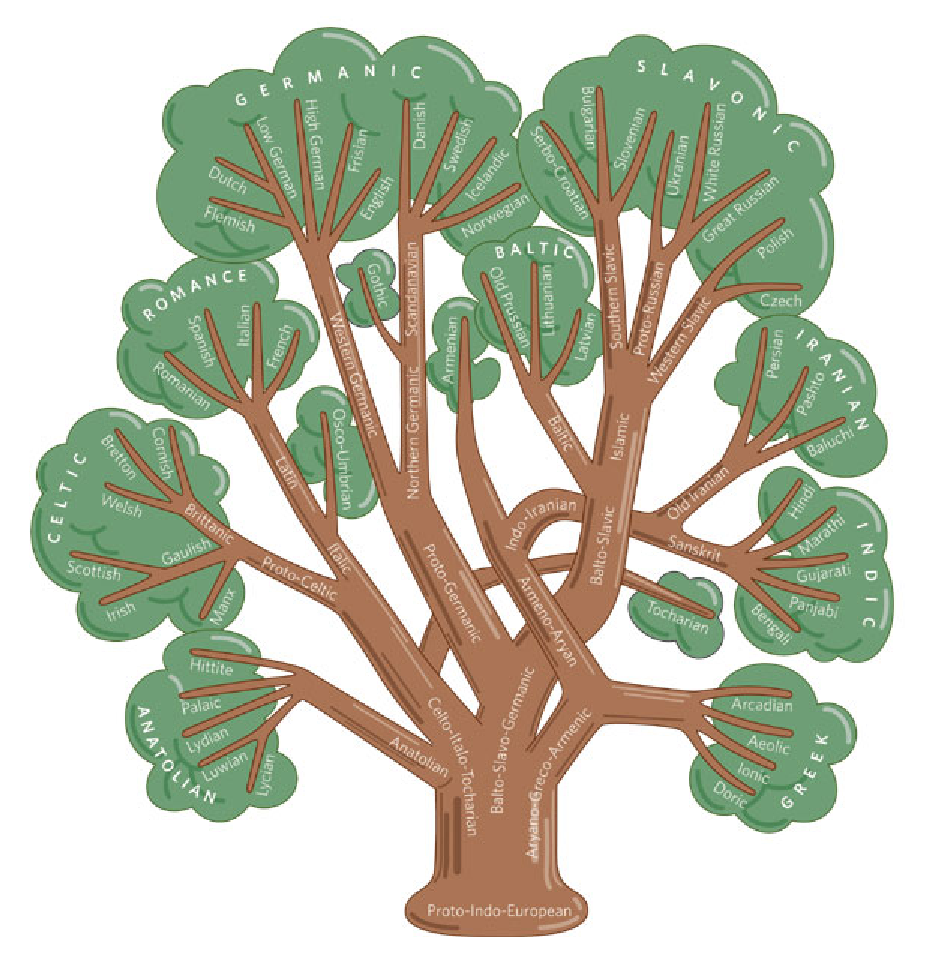
\includegraphics[width=\textwidth]{Pictures/indoeuropaeisch}
% \caption{\label{fig-indo-european-fitch}Language tree according to \citet[\page 665]{Fitch2007a-u}}
% \end{figure}
Proto-Germanic formed between 2000 and
1000 BCE. Its origins are in the Baltic region, that is, in northern Germany and southern
Scandinavia. 
%AZ About 500 BCE, the area where it was spoken extended from the North Sea to Poland.
The first written documents are runes from about 300 CE and the Gothic Bible translation in the fourth century.
%AZ I reordered this somewhat
The First Germanic Sound Shift took place before the second century BCE. In that millennium the
Germanic languages developed different consonants from the other Indo-European languages. 

Wikipedia\footnote{
\url{https://en.wikipedia.org/wiki/Germanic_languages}. 19.10.2014
} provides the table in Figure~\vref{fig-history-relations-germanic} that depicts the development of
the Germanic languages.
\begin{figure}
\begin{sideways}
\includegraphics[width=.9\textheight]{Pictures/germanic-wikipedia}
\end{sideways}
\caption{\label{fig-history-relations-germanic}History and grouping of Germanic languages according to Wikipedia}
\end{figure}
Germanic is divided into East, West, and North Germanic. East Germanic existed in the form of Gothic
until about 1800 on the Crimea
%AZ(Crimean Gothic)
and is now totally extinct. 

West Germanic consists of 
\begin{itemize}
\item German, 
\item Yiddish, 
\item Luxembourgish, 
\item Pennsylvania Dutch, 
\item Low German, % Plattdeutsch or Niederdeutsch
\item Plautdietsch (also called Mennonite Low German), %
\item Dutch, 
\item Afrikaans, 
\item Frisian, and 
\item English.
\end{itemize}
The North Germanic languages are:
\begin{itemize}
\item Danish,
\item Swedish
\item Norwegian
\item Icelandic, and 
\item Faroese.
\end{itemize}


Table~\vref{tab-words-germanic} shows how similar the words from the main vocabulary of the Germanic
languages are:
\begin{table}
\centerfit{%
\begin{tabular}{lllllllll}
\hline\hline
Dutch & vader  & vier    & vol    & huis  & bruin  & uit & kruid     & muis\\
German        & Vater  & vier    & voll   & Haus  & braun  & aus & Kraut     & Maus\\
English       & father & four    & full   & house & brown  & out & crowd (?) & mouse\\
Frisian      & –      & fjouwer & fol    & hûs   & brún   & út  & krûd      & mûs\\
Swedish     & fader  & fyra    & full   & hus   & brun   & ut  & krut      & mus\\
Danish        & fader  & fire    & fuld   & hus   & brun   & ud  & krudt     & mus\\
Norwegian     & far    & fire    & full   & hus   & brun   & ut  & krydder   & mus\\
Iclandic     & faðir  & fjórir  & fullur & hús   & brúnn  & út  & –         & mús\\
\hline\hline
\end{tabular}
}
\caption{\label{tab-words-germanic}Words from the main vocabulary of some Germanic languages}
\end{table}

%% \section{Stammbaum der germanischen Sprachen}
%% 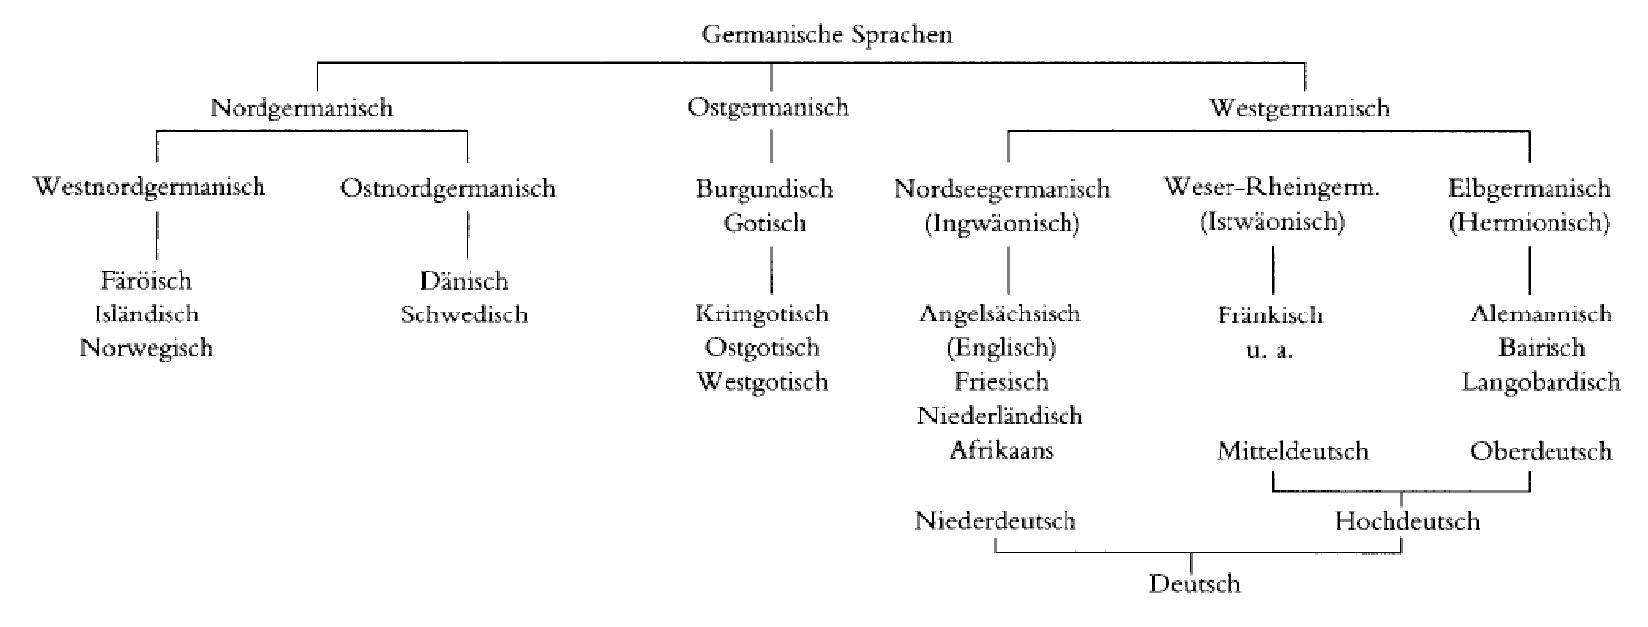
\includegraphics[width=\textwidth]{Pictures/stammbaum-germanisch}
%% aus \citew[S.\,251]{Bussmann2002a}





\section{The three branches of the Germanic family}

Proto-Germanic developed into the three main branches East, West, and North Germanic, approximately in
the first century CE. The reasons for this development were inherent variations in the respective
dialects, migration (language contact) and standardization. This book treats the structure of the
Germanic standard languages. This section is divided into three subsections that correspond to the
three main Germanic branches. I will sketch the historic developments that lead to the
languages spoken today. Many of the details that are covered in Figure~\ref{fig-history-relations-germanic} will be ignored.



\subsection{East Germanic}

The Goths emigrated from the Danish islands and South Sweden 
%AZ around is better than approximately; i am adjusting tenses 
100 BCE and met the
Vandals and other tribes.  \ili{Gothic} and \ili{Burgundian} and some smaller languages constituted the East Germanic branch, of which only Gothic got passed on.
After the decay of the Gothic empires Gothic died out. There were some remains on the peninsula
Crimea until about 1800. The West Gothic bishop Wulfila translated the Bible into Gothic. The
best-known version of it is the fragment Codex Argenteus, which belongs to the university library of
Uppsala. Figure~\vref{fig-Wulfila-Bibel} shows a picture of it.\footnote{
Taken from Wikipedia: \url{http://de.wikipedia.org/wiki/Bild:Wulfila_bibel.jpg}. 19.10.2014.
}
\begin{figure}
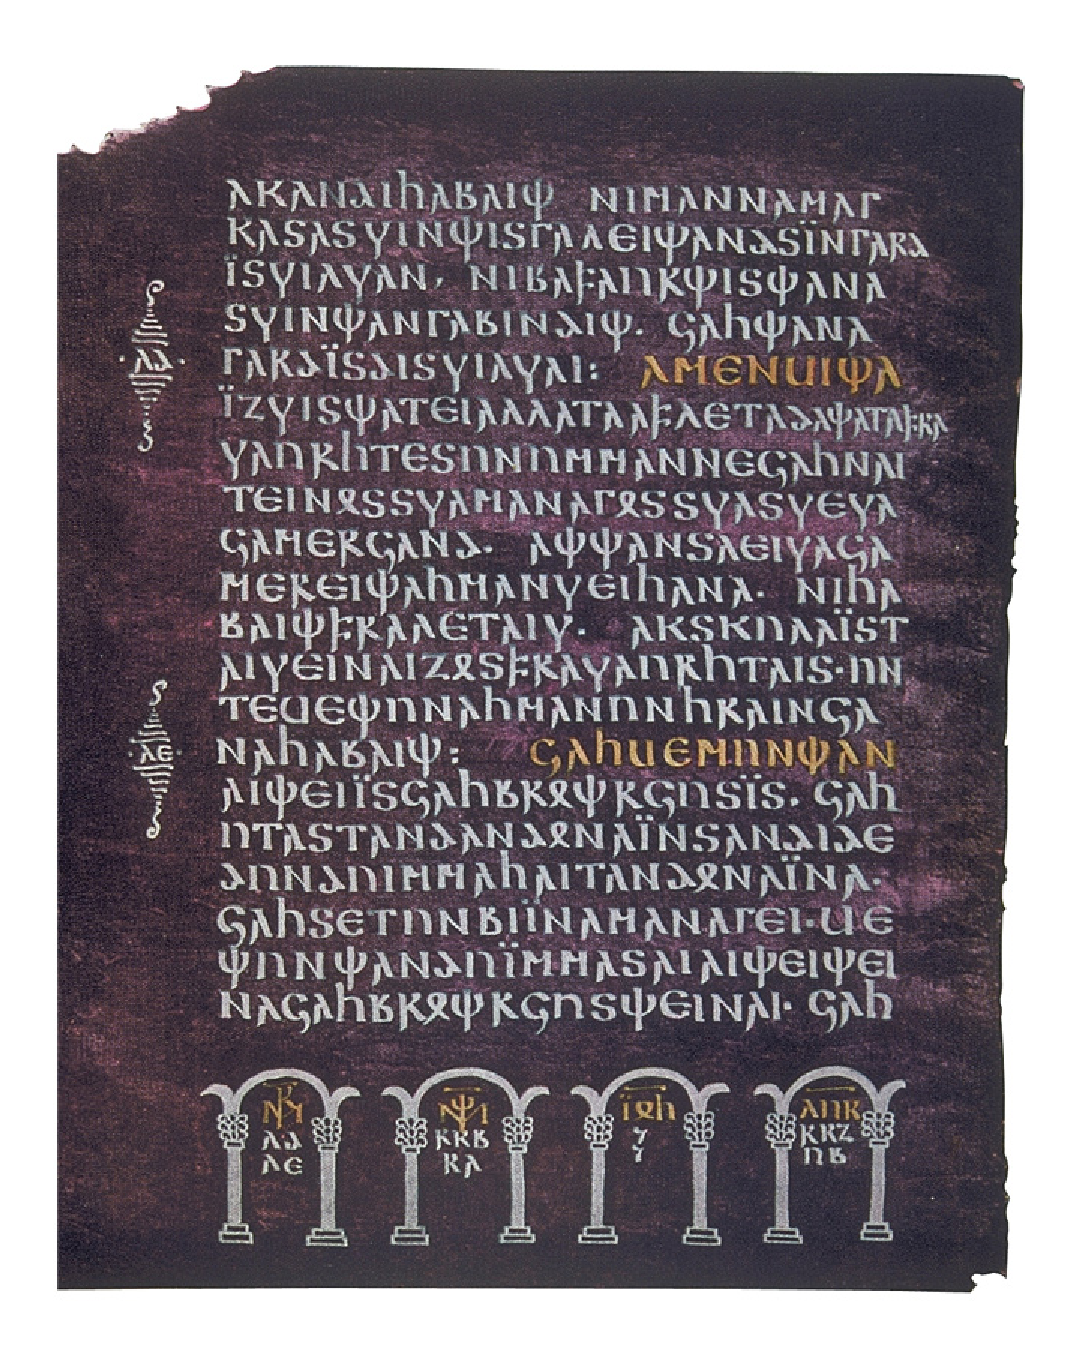
\includegraphics[width=53mm]{Pictures/Wulfila_bibel}
\caption{\label{fig-Wulfila-Bibel}The Wulfila Bible (Codex Argenteus), picture from Wikipedia}
\end{figure}



\subsection{North Germanic}

The first writings on runestones date back to the 6th century. The language of the Wikings %AZ Vikings in English
(800--1050) was rather homogeneous and it was only after this era that two branches were starting to
develop: the East-Scandinavian branch with Old-Danish and Old-Swedish and the West Scandinavian one
with Old-Norwegian and Old-Icelandic.


\subsubsection{Danish}

\ili{Danish} (dansk) is the official language of the \href{https://en.wikipedia.org/wiki/Denmark}{Kingdom of Denmark}, %AZ and the
second official language of the
Faroe Islands and of Greenland, Inuit\il{Inuit} being the first official language of
Greenland. Danish has about 5,5 million speakers. About 50,000 speakers live in \href{https://en.wikipedia.org/wiki/Schleswig-Holstein}{Schleswig-Holstein}, the northernmost of the federal states of Germany.
Danish is the Scandinavian language that drifted furthest away from the common Scandinavian roots.


\subsubsection{Swedish}

\ili{Swedish} (svenska) is the official language in Sweden with about 8,5 million native speakers. It is
the first language of about 300,000 Swedish-speaking Finns in Finland. Until the times of the
Vikings Danish and Swedish were almost indistinguishable. Starting from about 800 they started to
diverge. Since about 1300 there are obvious differences.



\subsubsection{Icelandic}


\ili{Icelandic} (íslenska) is the West Scandinavian language of Iceland since the %AZ its?
settlement over 1000
years ago. 
% Wikipedia 23.10.2014
There are about 325,000 native speakers. 97\,\% of the Icelandic population (325,000) has Icelandic as their
mother tongue and there are larger %AZ larger than what? I assume you mean large
groups of native speakers in Denmark, the USA, and Canada
(about 15,000 in total). 
There is almost no variation (no dialects).%AZ that is too strong there is actually quite a bit of variation but maybe it is correct to say that there is less variation than in other Germanic languages
The language is conservative, in the sense that Icelandic
is the language among the Germanic languages that best preserved the Germanic vocabulary and inflection.
In the beginning there were almost no differences between Norwegian and Icelandic but then %AZwhen?
the
languages diverged.

\subsubsection{Norwegian}

There are two varieties of \ili{Norwegian} (norsk): Danish-Norwegian (bokmål) and New-Norwegian (nynorsk, landsmål). 
Both are official languages of Norway and are used in parallel %AZ not clear what that means
. There are about 4,3 million
speakers.
From 1380 to 1814 Danish was the written language and local dialects were spoken %AZ in Norway. It deeveloped into the bokmål standard
%. Hence, a Norwegian
A standard %AZ that is less influenced by Danish was
%had to be 
developed%. This was done 
by Ivar Aasen (1813--1896), 
%who developed
Nynorsk. Nynorsk got an official status in 1885. Bokmål `book tongue' is the first language of most
of the Norwegians.

\subsubsection{Faroese}

\ili{Faroese} (føroyskt) is -- %AZ as well as Danish -- the
an official language of the Faroe Islands. There
are about 47,000 speakers. The Faroe Islands belong to Denmark since 1816. Since 1948 they are a
self-governing country within the \href{https://en.wikipedia.org/wiki/Danish_Realm}{Danish Realm}.
Faroese has a strong Danish influence. The first manuscript transmission is as recent as 1773 and
even 
%AZ after that date instead of then 
there are not many written documents 
%AZ i would leave this out: (in contrast to Icelandic).And put something in the Icelandic section


\subsection{West Germanic}


Opinions on the question whether West Germanic developed from a single source or not differ. Some authors
assume that the West Germanic languages do not have a common root, but instead developed from the
following three unrelated branches of dialect groups (for instance \citealp[\page 17--18]{Robinson1992a-u} and
\citealp[\page 9]{HvDA94a}):
\begin{itemize}
\item North Sea Germanic %(Ingvaeonic, ancestral to Anglo-Frisian and also Old Saxon)
\item Weser-Rhine Germanic %(Istvaeonic, ancestral to Old Frankish, its successors Low Franconian and several dialects of Old High German)
\item Elbe Germanic %(Irminonic, ancestral to several dialects of Old High German, most probably including the extinct Langobardic language).
\end{itemize}
Other authors assume that these three branches had a common ancestor (see Figure~\ref{fig-history-relations-germanic}).

There is no unique mapping of these dialect groups to the languages spoken today.





\subsubsection{German}

\ili{German} is the official language of
\begin{itemize}
\item Germany (about 80 million speakers), 
\item Austria (about 7,5 million speakers), 
\item Liechtenstein (about 15,000 speakers), 
\item Switzerland (4,2 million of 6,4 million Swiss residents),
\item Northern Italy/South Tyrol (about 270,000 speakers), 
\item Belgium (about 65,000 speakers), and
\item Luxembourg (about 360,000 speakers).
\end{itemize}
Luxembourg has next to German also 
%AZ leave out the original language, not clear what original means here
Luxembourgish and French as official
languages.

There are about 97 million speakers of German, about, 90 of those are native speakers and 7 million
have German as their second language.
% = Migrationshintergrund
% Quelle Wikipedia 15.10.2013
Approximately 80 million speakers speak German as a foreign language, about 55 Million of these live
in the European Union.%AZ It is a bit awkward to get these details for German but not for all the other languages

There are three main national variants (Germany, Austria, Switzerland). In other countries German is
%AZ leave out usually 
a minority language. There are two large dialect groups: Low German (Plattdüütsch,
Nedderdüütsch;in Standard German: Plattdeutsch or Niederdeutsch; %AZ this is clear as mud: do you want to say that Dutch is part of low Saxon or as most people do that low saxon are the dialects ofGerman that are spoken in in the Netherlands? I would say: Nedersaksisch or Low Saxon, a group of dialects spoken in the Netherlands, southern Danmark and northwestn Germany
) and High German (varieties of German spoken south of the Benrath and Uerdingen isoglosses).
%\todostefan{more}

% Wikipedia
%% The High German languages or High German dialects (German: Hochdeutsche Dialekte) comprise the varieties of German spoken south of the Benrath and Uerdingen isoglosses in central and southern Germany, Austria, Liechtenstein, Switzerland, and Luxembourg as well as in neighboring portions of Belgium (Eupen-Malmedy) and the Netherlands (Southeast Limburg), France (Alsace and northern Lorraine), Italy (South Tyrol), and Poland (Upper Silesia). They are also spoken in diaspora in Romania, Russia, the United States, Brazil, Argentina, Chile, and Namibia.

%% The High German languages are marked by the High German consonant shift, separating them from Low German and Low Franconian (Dutch) within the continental West Germanic dialect continuum.


%% Wikipedia

%% Middle Low German was the lingua franca of the Hanseatic League. It was the predominant language in Northern Germany. This changed in the 16th century: in 1534 the Luther Bible was published. This translation is considered to be an important step towards the evolution of the Early New High German. It aimed to be understandable to a broad audience and was based mainly on Central and Upper German varieties. The Early New High German language gained more prestige than Low German and became the language of science and literature. Around the same time, the Hanseatic league, based around northern ports, lost its importance as new trade routes to Asia and the Americas were established, while the most powerful German states of that period were located in Middle and Southern Germany.

%% The 18th and 19th centuries were marked by mass education in Standard German in schools. Gradually Low German came to be politically viewed as a mere dialect spoken by the uneducated. Today Low Saxon can be divided in two groups: Low Saxon varieties with a reasonable standard German influx[clarification needed] and varieties of Standard German with a Low Saxon influence known as Missingsch. Sometimes, Low Saxon and Low Franconian varieties are grouped together because both are unaffected by the High German consonant shift. However, the proportion of the population who can understand and speak it has decreased continuously since World War II.


%% Wikipedia
%% High German is divided into Central German, High Franconian (a transitional dialect), and Upper German. Central German dialects include Ripuarian, Moselle Franconian, Rhine Franconian, Central Hessian, East Hessian, North Hessian, Thuringian, Silesian German, Lorraine Franconian, Mittelalemannisch, North Upper Saxon, High Prussian, Lausitzisch-Neumärkisch and Upper Saxon. It is spoken in the southeastern Netherlands, eastern Belgium, Luxembourg, parts of France, and parts of Germany roughly between the River Main and the southern edge of the Lowlands. Modern Standard German is mostly based on Central German, although the common (but not linguistically correct) German term for modern Standard German is Hochdeutsch, that is, High German.

%% The Moselle Franconian varieties spoken in Luxembourg have been officially standardised and institutionalised and are usually considered a separate language known as Luxembourgish.

%% The two High Franconian dialects are East Franconian and South Franconian.

%% Upper German dialects include Northern Austro-Bavarian, Central Austro-Bavarian, Southern Austro-Bavarian, Swabian, East Franconian, High Alemannic German, Highest Alemannic German, Alsatian and Low Alemannic German. They are spoken in parts of the Alsace, southern Germany, Liechtenstein, Austria, and the German-speaking parts of Switzerland and Italy.

%% Wymysorys is a High German dialect of Poland native to Wilamowice, and Sathmarisch and Siebenbürgisch are High German dialects of Romania. The High German varieties spoken by Ashkenazi Jews (mostly in the former Russian Empire) have several unique features, and are usually considered as a separate language, Yiddish. It is the only Germanic language that does not use the Latin script as the basis of its standard alphabet.


\subsubsection{Yiddish}

\ili{Yiddish} is one of many 
%Jewish languages --> languages spoken in the Jewish diaspora
. About 2 million people speak this language in various
regions of the world, most of them in the USA (1,25 Mill.). The number of Yiddish speakers was much
higher 100 years ago: 7 million speakers of Yiddish lived in Europe, most of them in Russia and in
Austria-Hungary. At most 75,000 Yiddish speakers are left in Western Europe. Yiddish has its roots
in medieval German with influences from \ili{Hebrew} and \ili{Aramaic}.




\subsubsection{Pennsylvania German}

\ili{Pennsylvania German} (Pensilfaanish, Deitsch), which is also known as Pennsylvanian Dutch has about 300,000
native speakers, who mainly live in the USA. The most important regions are Pennsylvania, Ohio, and
Indiana. Pennsylvania German is the result of immigration in the 17th and 18th century. Members of
various protestant religions (Mennonites, Pietists and so on) left Europe for 
% religious reasons  
but later immigrants 
%AZ that came 
for economic reasons followed.  The language is
based on Palatine dialects and is nowadays mainly spoken by Amish and Mennonites.




\subsubsection{Dutch}

\ili{Dutch} (Nederlands) is the  official language of the Netherlands and has about 15 million speakers in that country. Dutch is also one of the official languages of Belgium with about 6 million speakers.
%AZleave out: ; almost 4 million Walloones). 
Dutch is the sole official language and teaching language in Suriname, 
%AZ leave out: which is independent since 1975, 
% 60% of the population speak it as their mother tongue % wikipedia
% 24% speak it as a second language
and in \href{https://en.wikipedia.org/wiki/Aruba}{Aruba} and the \href{https://en.wikipedia.org/wiki/Netherlands_Antilles}{Netherlands Antilles}.

%In Aruba, Curaçao and Sint Maarten, all parts of the Kingdom of the Netherlands, Dutch is the official language but spoken as a first language by only 7% to 8% of the population,[56] although most native-born people on the islands can speak the language since the education system is in Dutch at some or all levels.[57] The lingua franca of Aruba, Bonaire and Curaçao is Papiamento, a creole language that originally developed among the slave population. The population of the three northern Antilles, Sint Maarten, Saba, and Sint Eustatius, is predominantly English-speaking.[44]

\subsubsection{Afrikaans}

\ili{Afrikaans} is one of the official languages of South Africa since 1925, which has eleven official languages.
There are about 6,4 million native speakers in South Africa, which is about 15\,\% of the population,
and 150,000 in Namibia. Afrikaans developed since the 17th century from \ili{Dutch} dialects and is seen
as an independent language since somewhere between 1775 and 1850 \citep{denBesten2012a-u}.
% Oft wird gesagt, dass ab ca. 1775 von 'Afrikaans' gesprochen werden kann (Den Besten spricht aber noch vom 'Proto-Afrikaans'). Die Übergänge vom Kap-Niederländischen zum Afrikaans sind natürlich fließend, aber um die Zeit herum, gibt es doch schon genügend dokumentierte Unterschiede, um zu sagen, dass Afrikaans eine eigenständige Sprache geworden ist. Allerspätestens ab Mitte des 19. Jahhunderts ist dann aber auf jeden Fall eine eigene Sprache anzusetzen; da sind sich alle einig. Und 1925 wird das dann ja auch offizielle Amtssprache. 
The various %AZ African
languages spoken in
the area interacted with Afrikaans 
%AZ leave out: and its origins and resulted in a structural simplification in comparison to Dutch
. Today English has a strong influence.



\subsubsection{Frisian}

The three varieties of \ili{Frisian} are mutually not intelligible. There is North Frisian spoken by
about 10,000 speakers mainly on the north Frisian islands Amrum, Sylt, and Helgoland. East Frisian
is extinct with the exception of Saterlandic, which is spoken in the three villages of Saterland
(Landkreis Cloppenburg) by between 1,000 and 2,500 people.
% https://www.taz.de/!5834717 Inseln
West Frisian is spoken in the northern Dutch province Fryslân (Friesland) and has about 350,000
native speakers.



\subsubsection{English}

All over the world \ili{English} had about 570 million speakers at the end of the 20th century 
%AZ all over the world 
(337 million native speakers, 235 million speakers with English as the second language). The countries with the most native speakers are listed below: 
\begin{itemize}
\item USA: 227 million,
\item Great Britain: 57 million,
\item Nigeria: 43 million, 
\item Canada: 24 million,
\item Australia: 17 million,
\item Ireland: 3,5 million,
\item New Zealand: 3,2 million.
\end{itemize}
There are many national variants, which differ mostly in pronunciation.
%AZ it is not clear to me what the difference is between people that speak a language as a second language and people that have active knowledge of a language
Between 1 and  1,5 billion people have active or passive knowledge of English.
English is an official language in 59 states. It is the most important scientific language.




%      <!-- Local IspellDict: en_US-w_accents -->


%% -*- coding:utf-8 -*-

\settowidth\jamwidth{(German)}


\chapter{Phenomena}


This chapter deals with variation in the Germanic languages in what is often called the Core
Grammar, that is in sentences of the \emph{John loves Mary} variety.\footnote{%
  \citet[\page 7--8]{Chomsky81a} suggests dividing grammars of natural languages into a core part and a periphery.
All regular parts belong to the core. The core grammar of a language is assumed to be an instance of
Universal Grammar (UG), the genetically determined innate language faculty of human beings. Idioms
and other irregular parts of a language belong to the periphery. This book deals with phenomena
usually assumed to be the core without assuming this core/periphery distinction and without assuming
an UG \citep{MuellerKernigkeit,MuellerCoreGram}.
} We will look at differences in
the verb position (verb before object and object before verb), the verb second property, which
all of the Germanic languages with the exception of English have, the ordering of subjects and
obejcts with respect to each other, the placement of adverbials, the existence/non-existence of
verbal complexes, the obligatoriness/absence of subjects, passive including the personal and
impersonal passive, expletive pronouns and various ways to mark the \isi{clause type}, that is, to signal
whether a certain clause is an assertion, a question or an embedded clause.

A note of caution is necessary here: especially the following three subsections are potentially
confusing. A language like German will be categorized as an Subject-Object-Verb language, a verb-second language and
a language with free constituent order \citep{Haftka96a}. This sounds contradictory but it is not. The respective
classifications refer to properties of languages as such not to the form of single sentences.

\section{Order of subject, object and verb}
\label{sec-intro-svo}

The langauges of the world can be classified according to the order of subject, object, and verb
that is dominant \citep{Greenberg63a-u}. In order to make languages comparable a very general definition of grammatical
functions like subject and object is used
for such a classification. The definition is based on semantic properties: subjects are those
arguments that are agentlike and objects are arguments that are rather patient like. This definition
is not always identical to the language-particular definitions. For instance, if one follows the
semantic definition, the phrase \emph{der
  Aufsatz} `the paper' in (\mex{1}) is the subject although it is inanimate and not an agent: 
\ea
\gll Der Aufsatz interessiert mich.\\
     the paper   interests    me\\
\glt `I am interested in the paper.'
\z
The language-particular definition of subject in German (and the Germanic languages in general)
rather refers to properties like nominative case, subject-verb-agreement, and control. We will deal with this in more
detail in Section~\ref{sec-subj-properties}.

Figure~\vref{fig-sov-wals} shows the dominant order of subject, object, and verb among the world's languages.
According to \citet{Dryer2013a} the dominant order is defined as follows:

%Dominante Abfolge (Dryer: Determining Dominant Word Order):
\begin{quote}
Where a language is shown on one of the word order maps as having a particular order as the dominant
order in the language, this means that it is either the only order possible or the order
that is more frequently used. \citep{Dryer2013a}
\end{quote}
%
%% I base my classification of Macushi here on the frequency counts, and since no order is more than
%% twice as frequent as the next most frequent order, I treat this language as lacking a dominant order
%% of subject, object, and verb.
%
%% Deutsch, Niederländisch und Friesisch sind V2-Sprachen, that is die SVO- und SVAuxOV-Stellungen kommen
%% durch die Voranstellung des Verbs zustande, die eine Funktion hat. Wir zählen diese Sprachen also
%% mit zu den SOV-Sprachen.
%
\begin{figure}
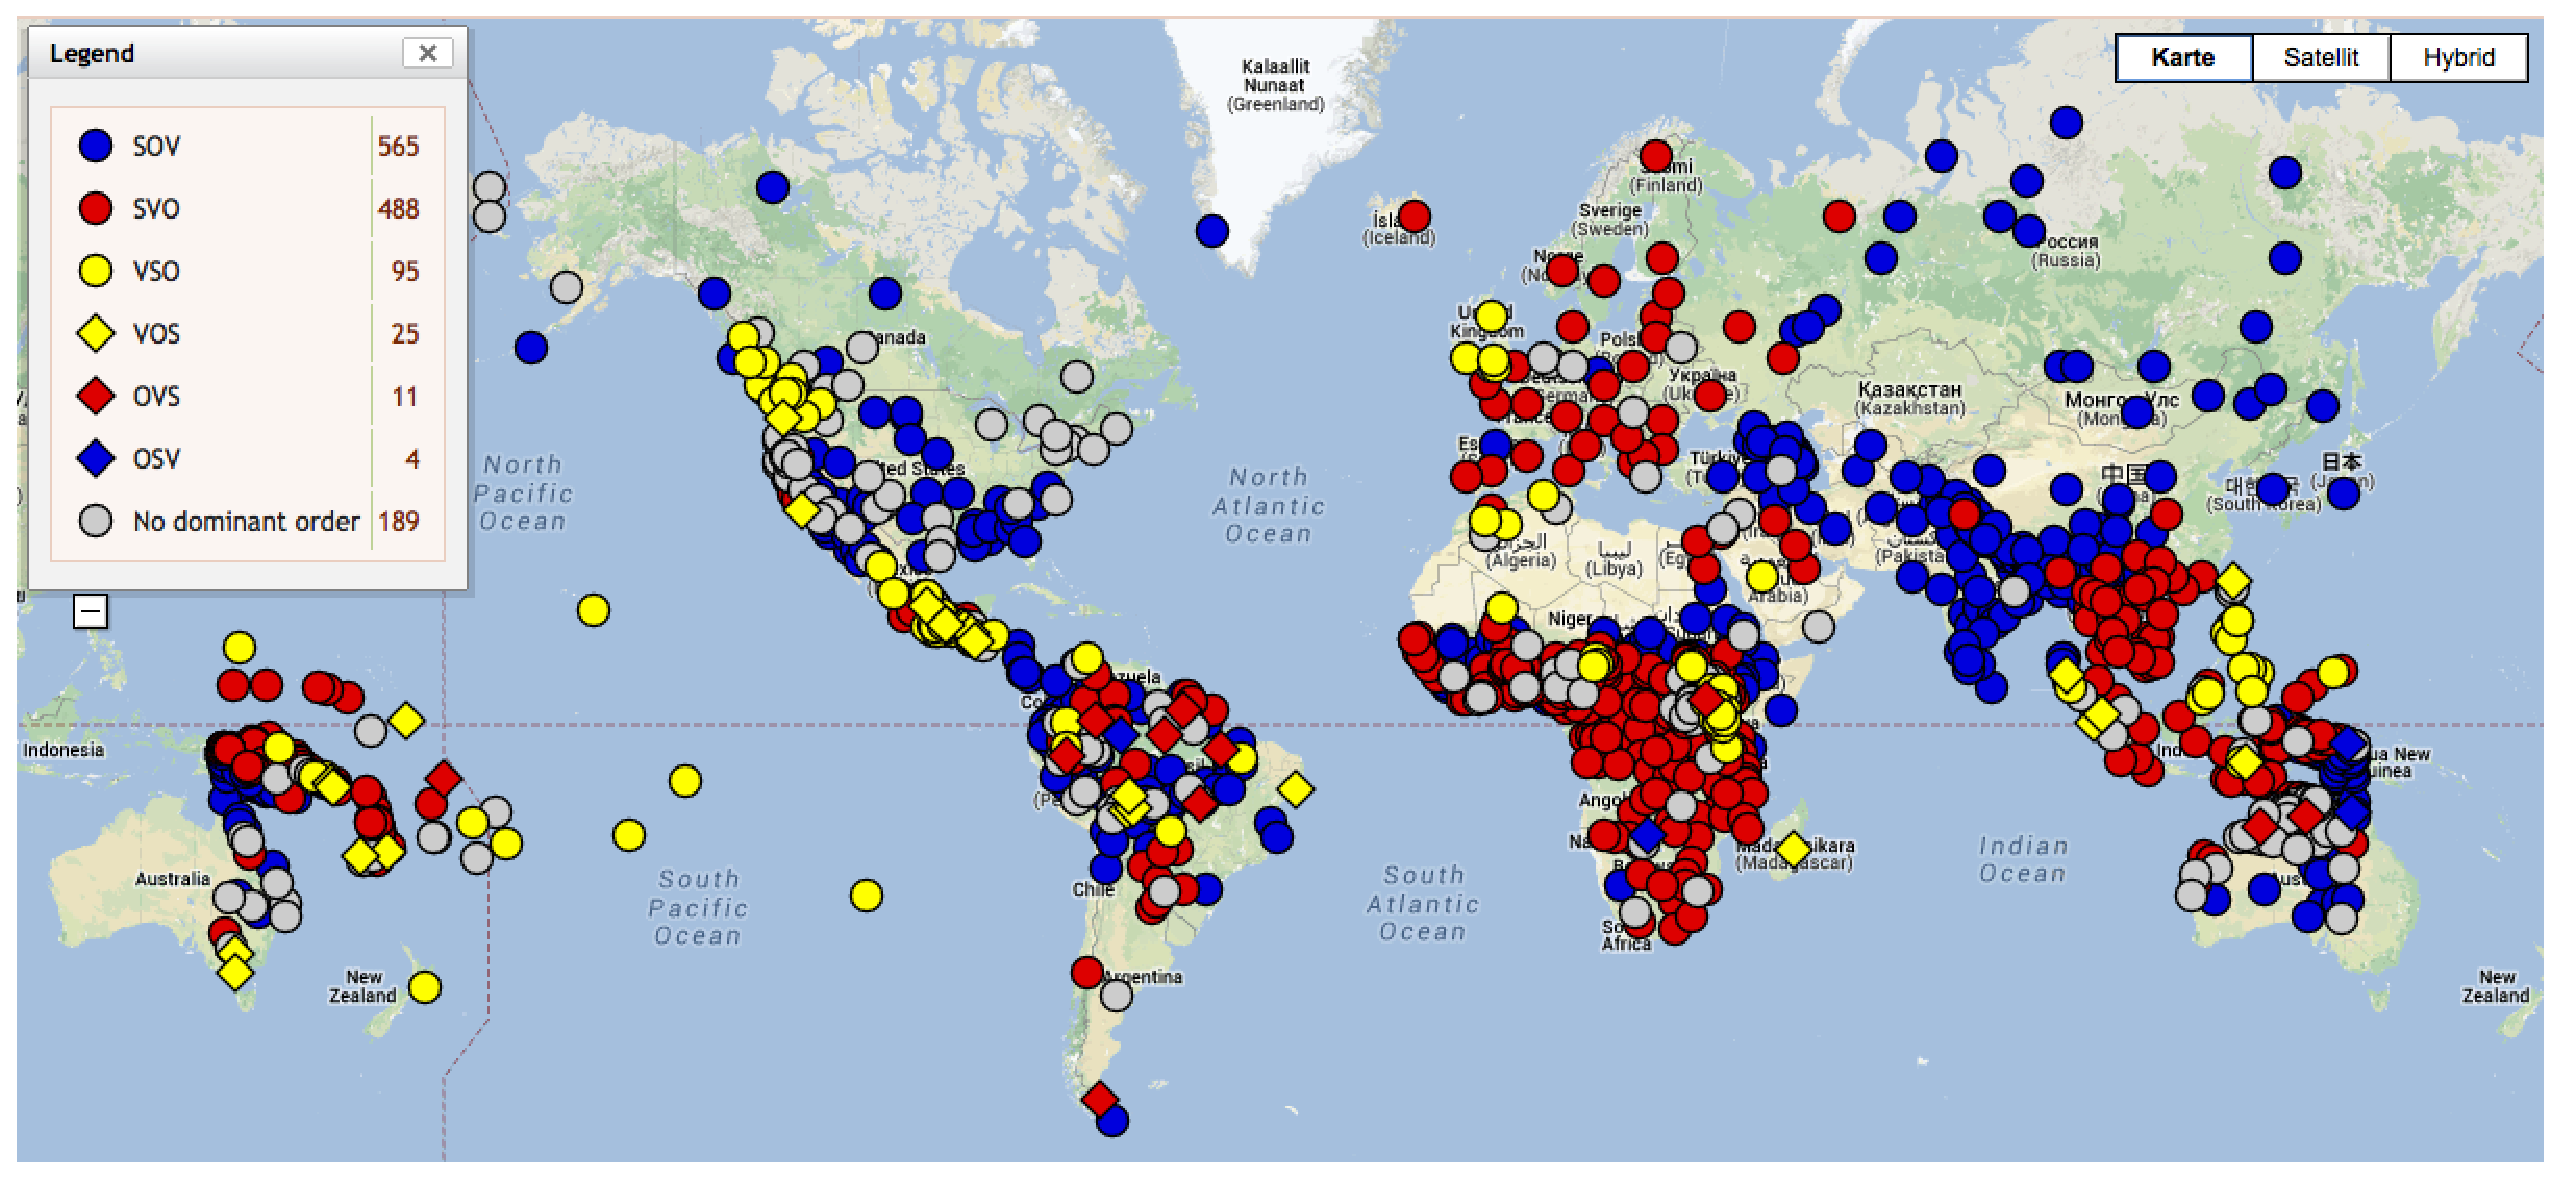
\includegraphics[width=\textwidth]{Pictures/WALS-SOV}
\caption{\label{fig-sov-wals}\citet[Section~1]{Dryer2013c}: Feature 81A: Order of subject, object and verb, The World Atlas of Language Structures} 
\end{figure}

If we zoom in to display the European languages we get Figure~\vref{fig-sov-wals-europe}.
\begin{figure}
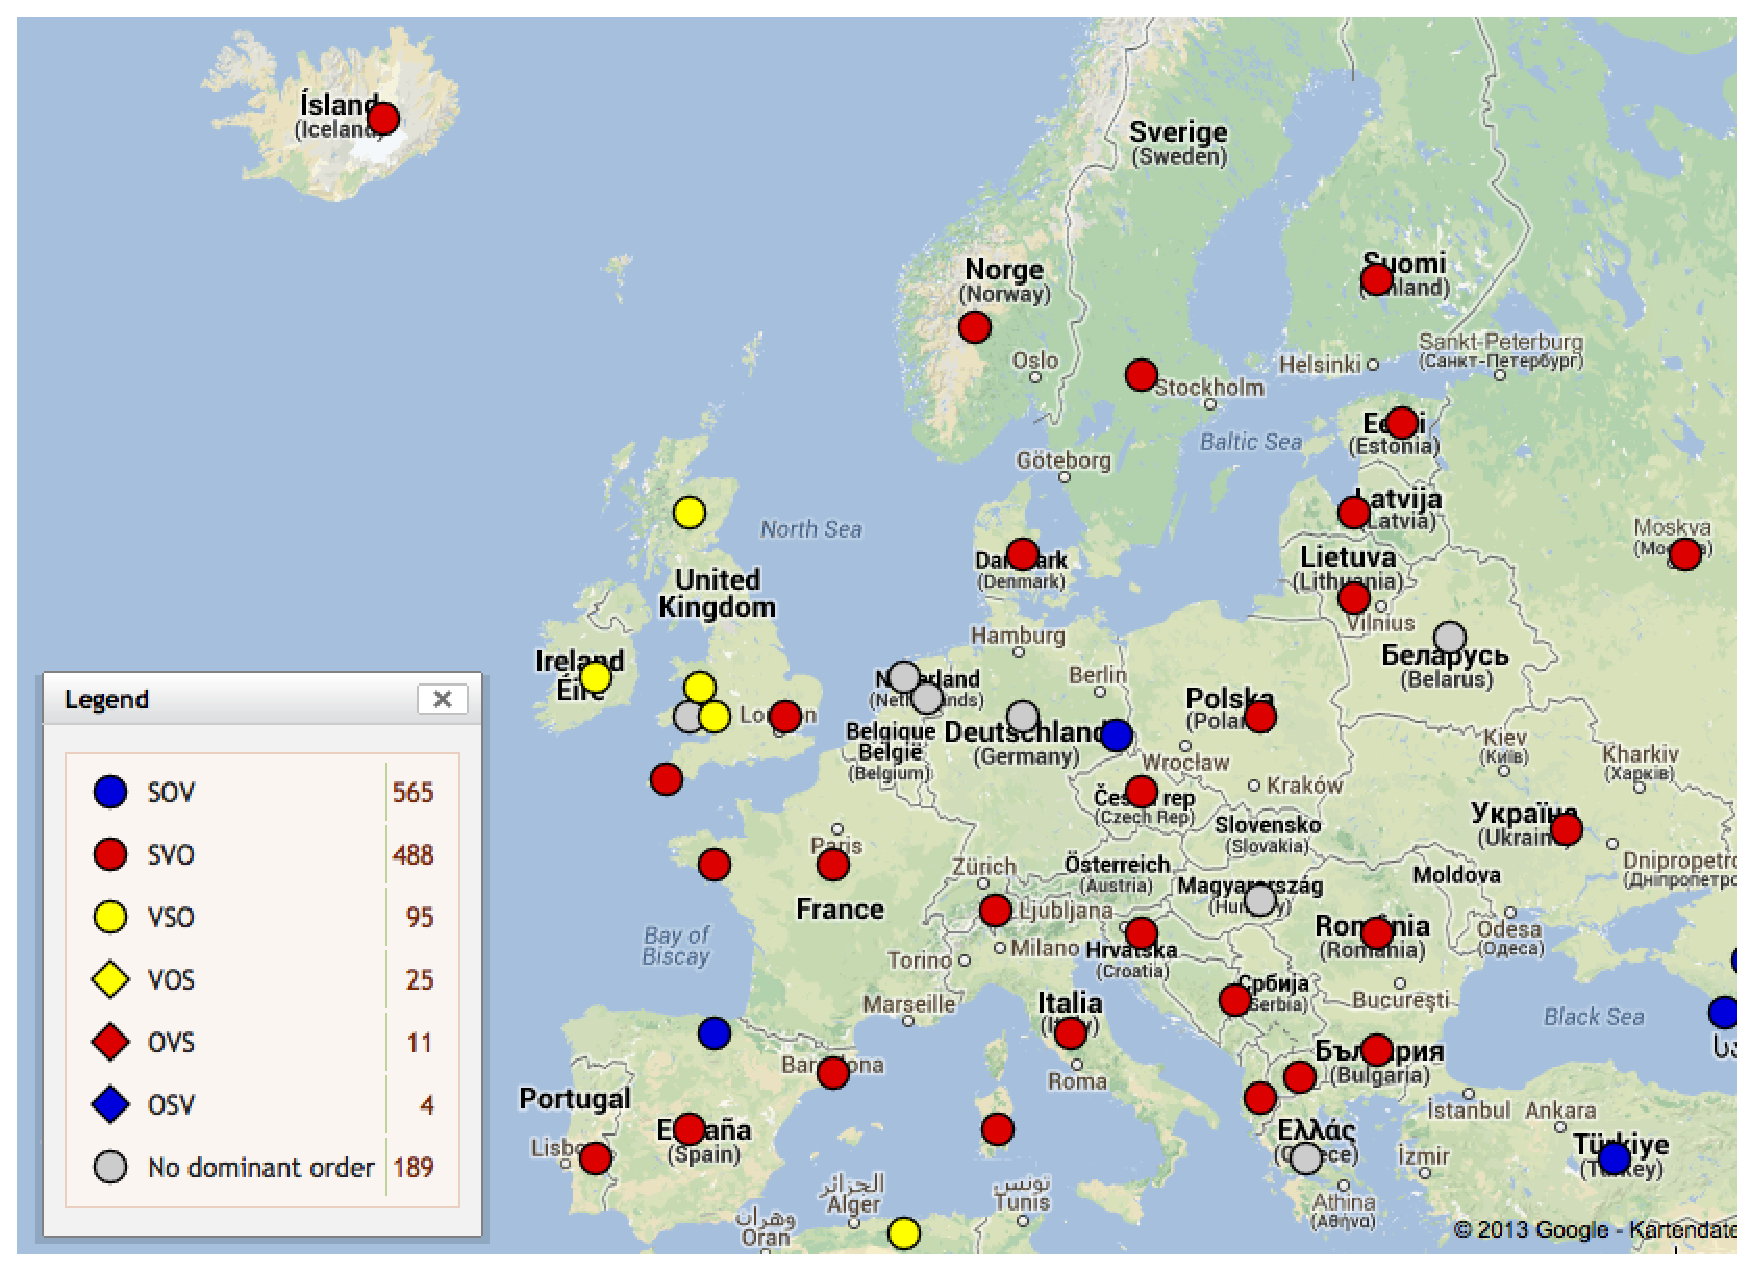
\includegraphics[width=.898\textwidth]{Pictures/WALS-SOV-Europa}
\caption{\label{fig-sov-wals-europe}Dominant orders of subject, object, and verb in Europe}
\end{figure}
According to the WALS the languages Iclandic, Norwegian, Swedish, Danish, and English are SVO
languages. Dutch, German, and Frisian, however, are marked in grey, that is, these languages are
marked to have no dominant order.\footnote{
  \citet[\page 87]{Greenberg63a-u} listed German and Dutch among the SVO languages.%
} According to Figure~\vref{fig-sov-wals-europe-two} these languages
have two dominant orders, namely SOV and SVO.
\begin{figure}
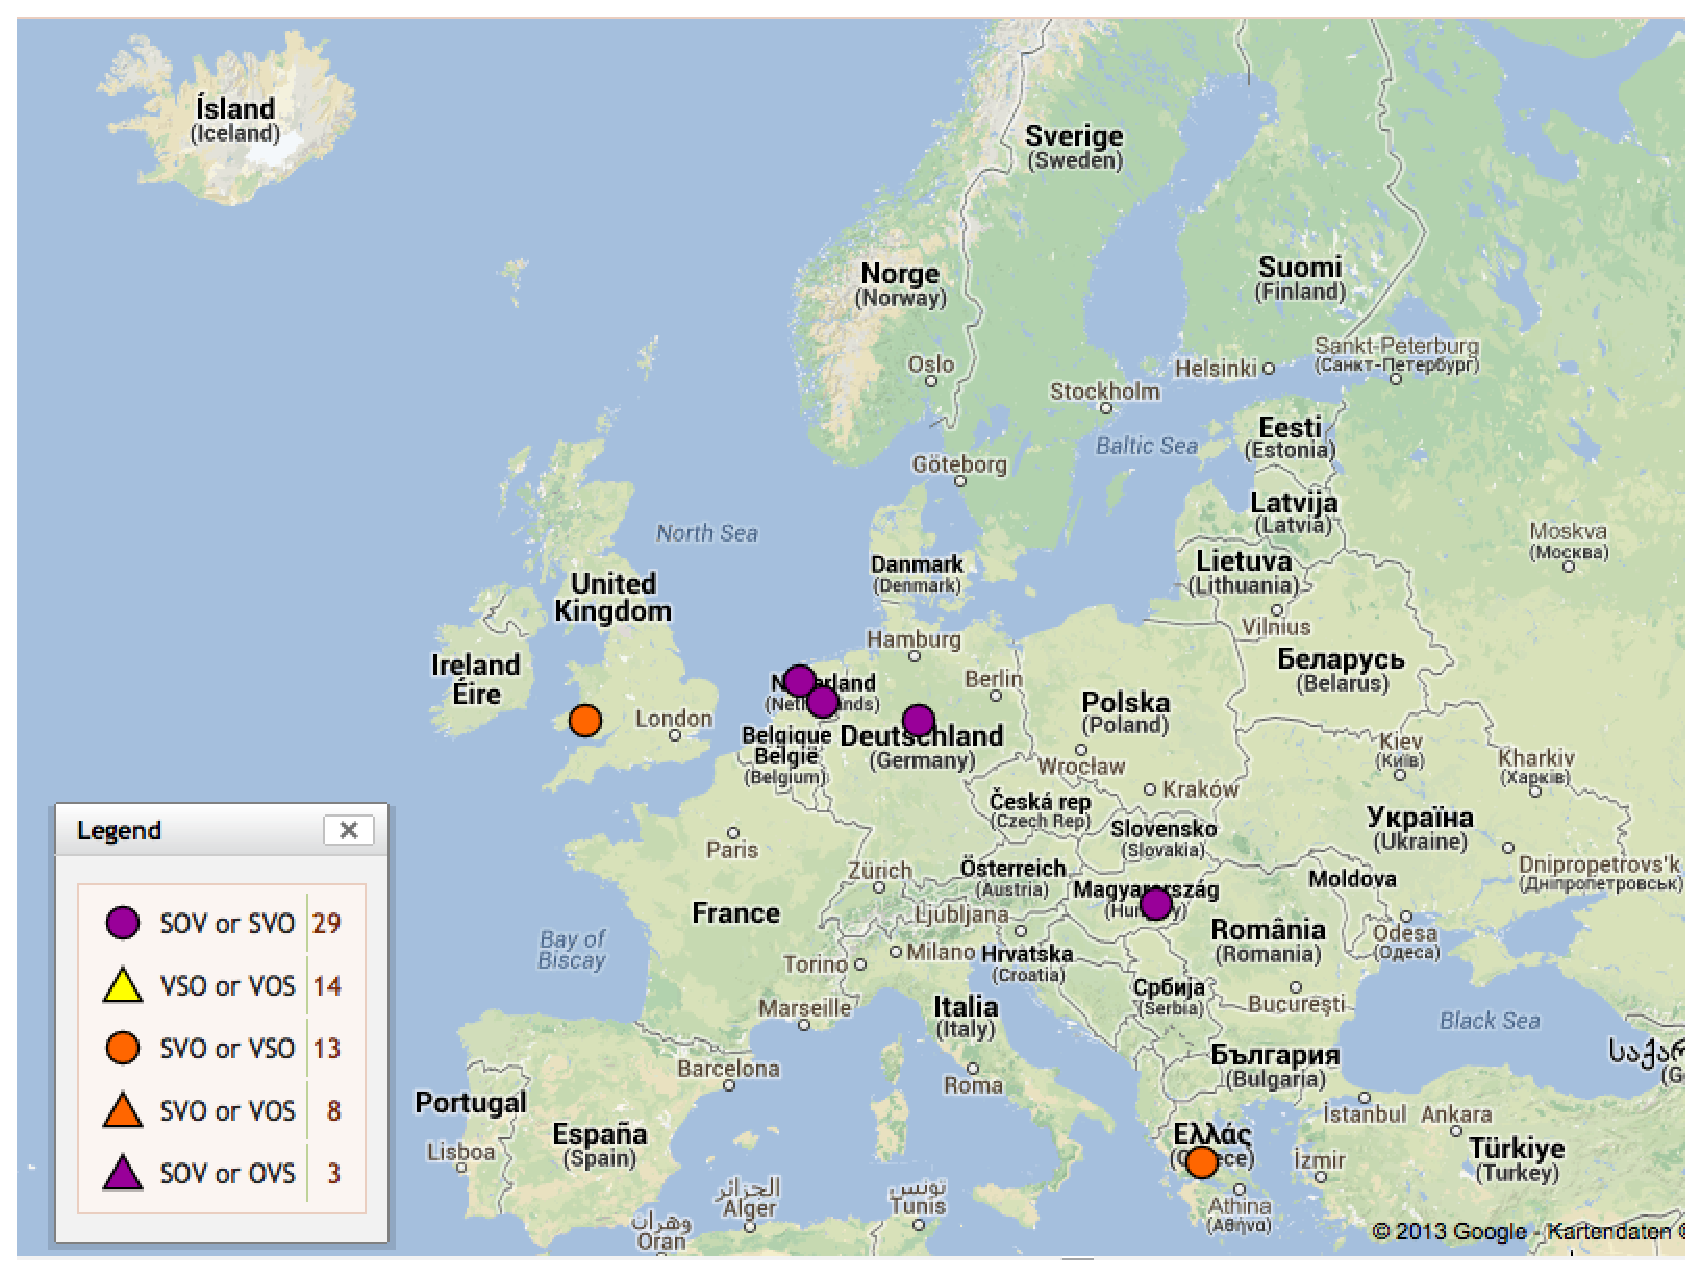
\includegraphics[width=.898\textwidth]{Pictures/WALS-SOV-Europa-no-dominant}
\caption{\label{fig-sov-wals-europe-two}%Dryer: Feature 81b: 
Two dominant orders of subject, object, and verb \citep[Section~3]{Dryer2013c}}
\end{figure}
%% https://wals.info/chapter/81
%% A third subtype of language lacking a dominant order consists of languages in which different word orders occur but the choice is syntactically determined. For example, in German and Dutch, the dominant order is SVO in main clauses lacking an auxiliary and SOV in subordinate clauses and clauses containing an auxiliary (see below for examples). Because this results in both orders being common, neither order is considered dominant here and these two languages are shown on the map as lacking a dominant word order. In general, if the word order varies according to whether there is an auxiliary verb, the language is shown on the map as lacking a dominant order. Another language whose word order depends both on whether there is an auxigermliary and whether the clause is a main clause is Dinka (Nilotic; Sudan): like German, the order is SVO in main clauses without an auxiliary, SAuxOV in main clauses with an auxiliary, but it is VSO in subordinate clauses without an auxiliary and AuxSOV in subordinate clauses with an auxiliary (Nebel 1948: 9, 25, 42, 75, 82).
The reason for this classification is that \citet[Section~1]{Dryer2013c} distinguishes between sentences in which the finite
verb is the main verb (\mex{1}a) and sentences in which the finite verb is an auxiliary as in (\mex{1}b):
\eal
\ex 
\gll Kim sieht den Mann.\\
     Kim sees the man\\
\glt `Kim sees the man.'
\ex
\gll Kim hat den Mann gesehen.\\
     Kim has the man seen\\
\glt `Kim has seen the man.'
\zl
According to Dryer the pattern for (\mex{0}a) is SVO and the one for (\mex{0}b) is SAuxOV, where Aux
stands for the auxiliary verb. Like
\citet{Greenberg63a-u}\footnote{%
  See \citew[\page 20--21]{HoehleTopo}.
}, Dryer counts the latter pattern as SOV order. The question is whether it is adequate to ignore auxiliaries
in the examination of constituent order. The auxiliary \emph{hat} `have' in (\mex{0}b) syntactically
behaves like the full verb \emph{scheint} `seems' in (\mex{1}):
\ea
\gll Kim scheint den Mann zu sehen.\\
     Kim seems   the man  to see\\
\glt `Kim seems to see the man.'
\z
So, here we would have an SVOV order, something that does not exist in the typology under discussion.
The languages in Figure~\ref{fig-sov-wals-europe-two} marked as not having a dominant order use the
verb position to mark the clause type: it is just the finite verb that is in first or second
position. Non-finite verbs are final: 
\ea
\gll Kim scheint den Mann gesehen zu haben.\\
     Kim seems   the man  seen to have\\
\glt `Kim seems to have seen the man.'
\z
In subordinate clauses we have both the finite verb and the non-finite verbs in final position while
we have the finite verb in initial position\footnote{%
  I use the term initial position to refer to the position the finite verb has in V1 or V2 clauses. The
  analysis of V2 and V1 involves fronting of the finite verb. In V2 clauses a constituent is fronted
  in addition.
} in questions and declarative main clauses.
A classification that is entirely based on counting patterns without taking auxiliary verbs and the
finiteness/non-finiteness distinction into account cannot tear these properties apart \citep[Section~3]{Hoehle83a}. In what follows we will have a look at clauses with
both finite and non-finite verbs. Such clauses reveal differences between OV and VO languages and I will argue that Afrikaans, Dutch,
German, and Frisian should be counted among the OV languages and that the other observable pattern
SVO is due to other properties of these languages, namely that they mark the clause type by verb
position and that they are verb second (V2) languages.\footnote{%
  The property of being a V2 language is independent of the SVO/SOV distinction. All Germanic
  languages except English are V2 languages. See Section~\ref{sec-phenomenon-v2} on V2.
}

When one builds more complex German sentences involving several verbs, the embedding verb is usually
realized to the right of the embedded verbs. This is shown in (\mex{1}). (\mex{1}a) shows a simple
sentence with a finite verb. If we form the perfect as in (\mex{1}b), the perfect auxiliary has to
follow the participle. The auxiliary is the finite verb and it determines the form of the
participle. Hence the finite verb is the verb that embeds the participle. This is indicated by the
lower number of \emph{hat} in comparison to \emph{gesehen}. If we build an even more complex
sentence by adding another verb, this verb will be serialized to the right of the present verbs
(\mex{1}c).  The Danish example in (\mex{2}c), quoted from \citet[\page 146]{Oersnes2009b}, corresponds to the
German example in (\mex{1}c).

\eal
\ex
\gll dass er ihn sieht$_1$\\
     that he him sees\\\jambox{(German)}
\glt `that he sees him'
\ex
\gll dass er ihn gesehen$_2$ hat$_1$\\
     that he him seen        has\\
\glt `that he has seen him'
\ex
\gll dass er ihn gesehen$_3$ haben$_2$ muss$_1$\\
     that he him seen        have     must\\
\glt `that he must have seen him'
\zl
\eal
\ex
\gll at   han ser$_1$ ham\\
     that he  sees    him\\\jambox{(Danish)}
\ex
\gll at   han have$_1$ set$_2$ ham\\
     that he  has      seen    him\\
\ex
\gll at   han må$_1$ have$_2$ set$_3$ ham\\
     that he  must   have     seen   him\\
\zl
%
As the examples in (\mex{0}) show, the verbs are added in front of the verbs they embed in
Danish. This is also the case for English as is evident from the glosses. In Danish and English the
verbs precede the object (\emph{ham}/\emph{him}) and in German they follow it (\emph{ihn}). 

\citet[Section~15.2]{Haider2020a} pointed out two further differences between the Germanic VO and OV languages:
particles precede verbs in OV languages and the same is true for resultative secondary
predicates. In VO languages particles and result predicates follow the verb. This is demonstrated by
the following two example sets:
\eal
\ex Peter will look up the information.
\ex 
\gll Peter wird die Information nachschlagen.\\
     Peter will the information \textsc{part}.beat\\\jambox{(German)}
\glt `Peter will look up the information.'
\zl
\eal
\ex Peter will fish the pond empty.
\ex 
\gll Peter wird den Teich leer fischen.\\
     Peter will the pond  empty fish\\\jambox{(German)}
\zl
(\mex{-1}a) shows that \emph{look} precedes the particle \emph{up}, while the verb \emph{schlagen}
`beat' has to follow the particle \emph{nach} in German. Similarly, the secondary resultative
predicate \emph{empty} follows the verb in (\mex{0}a), but \emph{leer} precedes the verb in
(\mex{0}b). Note that I used a future auxiliary in the examples in order to avoid side effects that
are due to the verb second property of German: in declarative main clauses the finite verb always
precedes particles and resultative predicates but this is due to the clause type (see Section~\ref{sec-phenomenon-v2}).

I will return to the SVO vs.\ SOV order in Chapter~\ref{chap-verb-position} and provide more
evidence that was used in the literature to argue for the OV status of languages like German and Dutch.


\section{V2}
\label{sec-phenomenon-v2}

The Germanic languages, with the exception of English, are so-called \emph{verb second languages} (V2
languages). The V2
property can be illustrated with the following German sentences. (\mex{1}) shows declarative main
clauses in which one of the constituents is fronted. (\mex{2}) shows parallel interrogative clauses.

\eal
\ex 
\gll Der Mann gibt der Frau morgen das Buch.\\
     the man  gives the woman tomorrow the book\\\jambox{(German)}
\glt `The man give the woman the book tomorrow.'
\ex 
\gll Der Frau gibt der Mann morgen das Buch.\\
     the woman gives the man tomorrow the book\\
\ex 
\gll Das Buch gibt der Mann der Frau morgen.\\
     the book gives the man the woman tomorrow\\
\ex 
\gll Morgen gibt der Mann der Frau das Buch.\\
     tomorrow gives the man the woman the book\\
\zl
\eal
\ex 
\gll Wer gibt der Frau morgen das Buch?\\  
     who gives the woman tomorrow the book\\\jambox{(German)}
\glt `Who gives the woman the book tomorrow?'
\ex 
\gll Wem gibt der Mann morgen das Buch?\\
     who gives the man tomorrow the book\\
\glt `Who does the man give the book to?'
\ex 
\gll Was gibt der Mann der Frau morgen?\\
     what gives the man the woman tomorrow\\
\glt `What does the man give the woman?'
\ex 
\gll Wann gibt der Mann der Frau das Buch?\\
     when gives the man the woman the book\\
\glt `When does the man give the woman the book?'
\zl
The finite verb is in second position in all the sentences in (\mex{-1}) and (\mex{0}).


English, in contrast, does not allow orders in which the object appears immediately before the
finite verb.

\eal
\ex[*]{ 
This man give I a book tomorrow.
}
\ex[*]{
This book give I a man tomorrow.
}
\ex[*]{
Tomorrow give I the man a book.
}
\zl 
Adverbials and objects can be fronted but then they have to appear before the clause consisting of
subject and verb and possibly other constituents.
\eal
\ex This book, I give the man tomorrow. 
\ex Tomorrow, I give the man a book.
\zl

Note also that fronting of objects is restricted to the secondary object for verbs with two objects
for some speakers \citep[\page 258]{Hudson92a-u}.\footnote{
  I use the terms \emph{primary object}\is{object!primary} and \emph{secondary object}\is{object!secondary} in order to avoid confusion that is sometimes
  caused by the terms \emph{direct}\is{object!direct} and \emph{indirect object}\is{object!indirect}. The primary object is the first object in English
  and the dative object of ditransitive verbs governing the dative in German. The secondary object
  is the second object in English and the accusative in German ditransitive constructions.
} So, while fronting of the secondary object in
(\mex{1}b) is permitted by all speakers, some speakers find extractions like the extraction of the
primary object in (\mex{1}c) unacceptable or marked.
\vspace{-\baselineskip}
\eal
\judgewidth{\%}
\ex[]{
We give children sweets.
}
\ex[]{
These sweets, we give children \_.
}
\ex[\%]{
These children, we give \_ sweets.
}
\zl
This is not the case in V2 languages: they are rather liberal as far as fronting
is concerned. Basically all constituents can be fronted, exceptions being reflexive
pronouns that are selected by inherently reflexive verbs (\mex{1}), expletive objects (\mex{2}), and certain modal
particles (\mex{3}). See also \citew[\page 159]{Hoberg81a} on inherently reflexive verbs and modal particles.
\eal
\ex[]{
\gll Maria erholt sich.\\
     Maria recovers \REFL\\\german
\glt `Maria recovers.'
}
\ex[*]{
\gll Sich erholt Maria.\\
     \REFL{} recovers Maria\\
}
\zl
\eal
\ex[]{
\gll Er bringt es bis zum Professor.\\
     he brings \expl{} until to.the professor\\\german
\glt `He makes it to professor.'
}
\ex[\#]{
\gll Es bringt er bis zum Professor.\\
     \expl{} brings he until to.the professor\\
} 
\zl
\eal
\ex[]{
\gll Er geht halt nicht.\\
     he goes \textsc{particle} not\\\german
\glt `He simply does not go.'
}
\ex[*]{
\gll Halt geht er nicht.\\
     \textsc{particle} goes he not\\
}
\zl

The element in front of the finite verb is not necessarily a clause mate of the finite verb. In
fact, it can belong to a deeply embedded head as is demonstrated by the following example from
German:
\ea
\gll [Über dieses Thema]$_i$ habe ich ihn gebeten, [[einen Vortrag \_$_i$ zu halten]?\footnotemark\\
     \spacebr{}about this topic  have I him asked \hspaceThis{[[}a talk {} to hold\\\german
\footnotetext{
\citew[\page 21]{HN89b}.
}
\glt `I asked him to give a talk about this topic.'
\z
The PP \emph{über dieses Thema} depends on \emph{Vortrag} `talk', which is part of the VP headed by
\emph{zu halten} `to hold', which is in turn embedded under \emph{gebeten} `asked'. Sentences like
(\mex{0}) show that V2 frontings cannot be analyzed as a simple reordering of the arguments of a
verb. While such an approach would work for the examples in (\mex{1}), it would not extend to other
cases in which the fronted element does not depend on the highest verb in the clause.
\ea
\gll Den Mann kennt er.\\
     the.\ACC{} man knows he\\
\glt `He knows the man.'
\z

The following examples from Danish (SVO) show that the property of being a V2
language is independent of the VO/OV property:
\eal
\ex 
\gll Max har læst bogen.\\
     Max has read book.\textsc{def}\\\danish
\ex
\gll Bogen har Max læst.\\
     book.\textsc{def} has Max read\\
\zl
The example in (\mex{0}a) shows that the object follows the verbs and (\mex{0}b) shows that the
object \emph{bogen} `the book' can appear in sentence initial position infront of the finite verb
\emph{har} `have'.

The V2 order is used in declarative main clauses throughout the Germanic languages (without
English). Some Germanic languages do not use V2 order in embedded clauses. For a discussion of
embedded interrogatives see Section~\ref{sec-embeeded-clauses}.

While English does not allow for the order object verb subject, which is possible in the other Germanic
languages due to V2 fronting, it allows for the fronting of the object in questions resulting in
structures that are parallel to what we know from the other Germanic languages:
\eal
\ex Which book did Peter read?
\ex Which book did Peter give to Mary?
\ex To whom did Peter give the book?
\zl
English used to be a V2 language but lost this property. The V2 in questions is a residue of earlier
stages of the language, which is why English is called a \emph{residual V2 language}\is{V2
  language!residual} \citep[\page 375]{Rizzi1990a-u}. 

V2 and verb fronting in general is a way to mark clause types in all Germanic languages. V2 sentence
can be declarative clauses in all Germanic languages except English and they can be questions in all
Germanic languages including English. In addition V2 sentences may be imperatives, as (\mex{1}) shows.
\ea
\gll Jetzt gib ihm das Buch!\\
     now give me the book\\\german
\glt `Give me the book now!'
\z
Sentences with the finite verb in first position (V1) can be yes/no questions or imperatives:
\eal
\ex
\gll Gibt er ihm das Buch?\\
     gives he him the book\\\german
\glt `Does he give him the book?'
\ex 
\gll Gib mir das Buch!\\
     give me the book\\
\zl
Of course the order of elements is not the only cue as far as the clause type is
concerned. Intonation and morphological marking of imperative forms plays a role as well.

The property of being a V2 language is exceedingly rare among the world's languages \citep[\page
  343]{Holmberg2015a}. Apart from the Germanic languages with the exception of 
Modern English \citep{HP86a-ed}, there are only \ili{Estonian} (Finno-Ugric, \citealp[\page 343]{Holmberg2015a}), \ili{Sorbian} \citep[entry~79]{Plank2003b-ed} (a Slavic language), the
Celtic languages \ili{Breton} \citep{BK2000a-u}, \ili{Cornish} \citep*[\page 287]{BTW2007a-u}, and Middle \ili{Welsh} \citep{Willis98a}, \ili{Old
  French} \parencites[Section~1.3]{Adams1987a-u}[Section~2.1.2]{Roberts93a-u}[Chapter~2]{Vance97a-u}, \ili{Old Spanish}
% Plank2003b-ed: and some other early Romance languages
%\citep{Fontana93a,Fontana97a}, 
\citep[Section~3.3.2]{Fontana97a-u}, 
\ili{Rhaeto"=Romance} \citep{Poletto2002a-u,Anderson2006a-u}, Kashmiri
\citep[Chapter~4]{Bhatt99a-u}, two dialects of \ili{Himachali}, which also belongs to Indo"=Aryan
and is spoken in regions adjacent to Kashmiri \citep{Hendriksen90a}, the Austronesian
languages \ili{Taiof} and \ili{Sisiqa} \citep[\page 495]{Ross2004a-u} and the Brazilian native
language \ili{Karitiana} from the language family Tupí \citep{Storto2003a-u}.
% This is mentioned in Bayer2010, but maybe it is like the australian languages.
% and the
%Uto-Aztekian language \ili{Tohono O'odham}, which is spoken in the southwest of the US and in northern Mexico.

% Estnisch 


\section{Scrambling}

While the constituent order in languages like English is rather fixed, languages like Dutch and
German allow a rather free permutation of arguments. In order not to contaminate the effects by
reorderings that are due to the V2 property, I use verb last sentences to illustrate the
phenomenon. Example (\mex{1}) shows the only possible order for subject and objects of a simple
ditransitive sentence without extraction:


\ea
because the man gives the woman the book \jambox{(English)}
\z
If speakers want to realize the secondary object \emph{the book} before the primary object \emph{the
  woman}, they have to use a prepositional object. This type of reordering is called
\emph{dative-shift} and an example is provided in (\mex{1}):
\ea
because the man gives the book to the woman \jambox{(English)}
\z
In contrast to this we have the German examples in (\mex{1}). These examples show that the noun
phrases can be freely permuted:
\eal
\ex 
\gll {}[weil]          der Mann der Frau das Buch gibt\\
     \spacebr{}because the man the woman the book gives\\\jambox{(German)}
\ex 
\gll {}[weil]          der Mann das Buch der Frau  gibt\\
     \spacebr{}because the man  the book the woman gives\\
\ex 
\gll {}[weil]          das Buch der Mann der Frau  gibt\\
     \spacebr{}because the book the man  the woman gives\\
\ex 
\gll {}[weil]          das Buch der Frau  der Mann gibt\\
     \spacebr{}because the book the woman the man  gives\\
\ex 
\gll {}[weil]          der Frau  der Mann das Buch gibt\\
     \spacebr{}because the woman the man  the book gives\\
\ex 
\gll {}[weil]          der Frau  das Buch der Mann gibt\\
     \spacebr{}because the woman the book the man  gives\\
\zl
Not all of these orders can be used in all contexts. Some of the examples require a special,
contrastive intonation. The orders can be sorted with respect to the number of contexts in which
they can be used. \citet{Hoehle82a} suggests calling the order that can be used in most contexts the
normal or unmarked order.




\section{The position of adverbials}


In languages like German and Dutch, the position of adverbials is rather free: the adverb \emph{gestern}
`yesterday' can appear anywhere between the arguments and the verb:
\eal
\ex
\gll weil der Mann der Frau das Buch \emph{gestern} gab\\ 
     because the man the woman the book yesterday gave\\\german
\glt `because the man gave the woman the book yesterday'
\ex 
\gll weil der Mann der Frau \emph{gestern} das Buch gab\\
     because the man the woman yesterday the book gave\\
\ex 
\gll weil der Mann \emph{gestern} der Frau das Buch gab\\
     because the man yesterday the woman the book gave\\
\ex 
\gll weil \emph{gestern} der Mann der Frau das Buch gab\\
     because yesterday the man the woman the book gave\\
\zl
Dutch has free order of adverbials as well \parencites[\page
4]{Koster99a-u}[Section~6]{Bouma2003a-u}. (\mex{1}) shows the Dutch examples corresponding to (\mex{0}):
% Bouma2003a:6
% \eal
% \ex
% \gll dat  Kim regelmatig haar moeder bezoekt\\
%      that Kim regularly  her  mother visits\\\dutch
% \glt `that Kim visit her mother regularly'
% \ex
% \gll dat  Kim haar moeder regelmatig bezoekt\\
%      that Kim her  mother regularly  visits\\
% \glt `that Kim visit her mother regularly'
% \zl
\eal
\ex
\gll omdat de man de vrouw het boek \emph{gisteren} gaf\\ 
     because the man the woman the book yesterday gave\\\dutch
\glt `because the man gave the woman the book yesterday'
\ex 
\gll omdat de man de vrouw \emph{gisteren} het boek gaf\\
     because the man the woman yesterday the book gave\\
\ex 
\gll omdat de man \emph{gisteren} de vrouw het boek gaf\\
     because the man yesterday the woman the book gave\\
\ex 
\gll omdat \emph{gisteren} de man de vrouw het boek gaf\\
     because yesterday the man the woman the book gave\\
\zl



In contrast, the position of the adverbials is rather restricted in SVO languages like Danish and
English. The adverbials usually are placed before or after the VP; that is, verb and objects form one
unit and adverbials attach to the left or to the right of this unit. (\mex{1}) provides an example:
\eal
\ex[]{
because the man {often} [gave the woman the book] \jambox{(English)}
}
\ex[]{
because the man [gave the woman the book] {often}
}
\ex[*]{
because the man [gave often the woman the book]
}
\ex[*]{
because the man [gave the woman often the book]
}
\zl
It is assumed that verb and objects form a structural unit, a verb phrase (VP). Adverbials may
attach to this VP forming a larger VP, which is than combined with the subject to form a complete sentence.

The following example, which is due to \citet[§ 8.20, 495]{QGLS85a-u}, shows that even in very
complex combinations of several verbs adverbs may be placed at the left periphery of a VP:
\ea
It [certainly [\sub{VP} may [possibly [\sub{VP} have [indeed [\sub{VP} been\\ {}[badly [\sub{VP} formulated]]]]]]]].
\z
This is different from the OV languages where verbs form a verbal complex which usually cannot be
interrupted by adverbs.
\eal
\ex[]{
\gll dass der Mann der Frau das Buch morgen geben dürfen muss\\
     that the man  the woman the book tomorrow give may must\\
\glt `that it must be possible that it is allowed that the man gives the woman the book tomorrow'
}
\ex[*]{
\gll dass der Mann der Frau das Buch geben morgen dürfen muss\\
     that the man  the woman the book give tomorrow may must\\
}
\ex[*]{
\gll dass der Mann der Frau das Buch geben dürfen morgen muss\\
     that the man  the woman the book give  may tomorrow must\\
}
\zl

\section{Embedded clauses}
\label{sec-embeeded-clauses}

This section deals with embedded clauses that are introduced by a complementizer and with
embedded interrogative clauses. The Germanic languages vary with respect to the verb placement in
these subordinate clauses and with respect to the question whether the embedded clauses are V2 or not.

\subsection{Embedded clauses introduced by a complementizer}

As was already mentioned Afrikaans, Dutch, German are SOV languages and this is shown in embedded
clauses that are introduced by a complementizer. (\mex{1}) is an example:

\ea
\gll Ich weiß, dass Max das Buch heute gelesen hat.\\
     I know that Max the book today read has\\
\glt `I know that Max read the book today.'
\z


%% Stellung der anderen Konstituenten ist frei:
%% \eal
%% \ex Ich weiß, dass das Buch Max heute gelesen hat.
%% \ex Ich weiß, dass das Buch heute Max gelesen hat.
%% \zl

English, beeing an SVO non-V2 language allows for SVO order only.
\ea[]{
I  know that Max has read the book yesterday. \jambox{(English)}
}
\z

Interestingly, Danish, also an SVO languauge, allows both SVO order (\mex{1}) and V2 order (\mex{2}) in clauses
preceeded by a complementizer:
\ea[]{
\label{ex-at-max-ikke-har}
\gll Jeg  ved, at   Max ikke  har læst   bogen          {i dag}.\\
     I know that Max not has read book.\textsc{def} today\\\jambox{(Danish)}
\glt `I know that Max did not read the book today.'
}
\z
%(Negation hilft, Verbstellung zu bestimmen)

\eal
\ex[]{
\gll Jeg  ved, at   {i dag} har Max ikke læst bogen.\\
     I    know that today   has Max not read book.\textsc{def}\\\jambox{(Danish)}
}
\ex[]{
\gll Jeg  ved, at   bogen          har Max ikke  læst {i dag}.\\
     I know that book.\textsc{def} has Max not read today\\
}
\zl
The example in (\ref{ex-at-max-ikke-har}) includes the negation in order to show that we indeed deal
with the SVO order here. Without the negation it is not clear whether non-V2 clauses are allowed in
clauses that are introduced by a complementizer since (\mex{1}a) has the finite verb in second
position. With the negation present, it is clear that we have a V2 clause if the negation follows
the finite verb and that we do not have a V2 clause if the finite verb follows the negation as in
(\mex{-1}) and hence is in third position.
\eal
\settowidth\jamwidth{(V2 or SVO)}
\ex 
\gll at Max har læst bogen\\
     that Max has read book.\textsc{def}\\\jambox{(V2 or SVO)}
\ex 
\gll at Max har ikke læst bogen\\
     that Max has not read book.\textsc{def}\\\jambox{(V2)}
\zl 
For complementizerless sentences the V2 order is the only one that is possible:
\eal
\settowidth\jamwidth{(V2 or SVO)}
\ex[]{ 
\gll Max har ikke læst bogen\\
     Max has not read book.\textsc{def}\\\jambox{(V2)}
}
\ex[*]{ 
\gll Max ikke har læst bogen\\
     Max not  has read book.\textsc{def}\\\jambox{(SVO)}
}
\zl 


Yiddish and Icelandic are SVO languages as well. The clauses that are combined with a
complementizer are V2:
\eal
\ex
\gll Ikh meyn  az   haynt hot Max geleyent dos bukh.\footnotemark\\
     I think that today has Max read the book\\\yiddish
\footnotetext{\citew[\page 58]{Diesing90a}.}
\glt `I think that Max read the book today.'

\ex% check!
\gll Ikh meyn  az   dos bukh hot Max geleyent.\\
     I think that the book has Max read\\

\zl
\todostefan{provide Icelandic example}

\citet[\page 75]{Maling90a-u}
\eal
\ex 
\gll Engum         datt í hug,  að   vert  væri að reyna til     að kynnast honum.\\
     no.one.\DAT{} fell to mind that worth was  to try   \PREP{} to know    him\\
\glt `It didn't occur to anyone that t was worth trying to get to know him.'
\zl

\subsection{Interrogative clauses}


The OV languages form subordinated interrogative clauses by preposing a phrase containing an
interrogative pronoun\footnote{
Most interrogative pronouns start with \emph{w} in German and \emph{wh} in English. Phrases
containing an interrogative pronoun are called \emph{w} phrases or \emph{wh} phrases,
respectively. Interrogative clauses are sometimes called \emph{w} clauses or \emph{wh} clauses.
} from an
otherwise SOV clause. (\mex{1}) shows a German example:
\eal
\ex 
\gll Ich weiß, wer heute das Buch gelesen hat.\\
     I know    who today the book read has\\\jambox{(German)}
\glt `I know who read the book today.'
\ex 
\gll Ich weiß, was Max heute gelesen hat.\\
     I know    what Max today read has\\
\glt `I know what Max has read today.'
\zl
Since languages like German allow for scrambling, senteces like those in (\mex{0}) could just be due
to the permutation of arguments of a head. However, the generalization about these \emph{w} clauses
is that an arbitrary \emph{w} element can be fronted. (\mex{1}) gives an example from German that
involves a nonlocal dependency:
\ea
\gll Ich weiß nicht, [über welches Thema]$_i$ er versprochen hat,~~~~~~~~ [[einen Vortrag \_$_i$] zu halten].\\
     I know not      \spacebr about which topic he promised has \hspaceThis{[[}a talk to  hold\\\jambox{(German)}
\glt `I do not know about which topic he promised to give a talk.'
\z
Here, the phrase \emph{über welches Thema} `about which topic' is an argument of \emph{Vortrag},
which is embedded in the VP containing \emph{zu halten} `to hold', which is in turn embedded under
\emph{versprochen hat} `promised has'. The generalization about interrogative clauses is that an
interrogative clause consists of a interrogative phrase (\emph{über welches Thema} `about which
topic') and a clause in which this interrogative phrase is missing somewhere (\emph{er versprochen
  hat, einen Vortrag zu halten} `he promised to give a talk').

In German the order of the other constituents is free as in assertive main clauses and embedded
clauses with a complementizer that were discussed earlier. 
\eal
\ex
\gll Ich weiß, was keiner diesem Mann geben würde.\\
     I know    what nobody this man give would\\\jambox{(German)}
\glt `I know what nobody would give this man.'
\ex 
\gll Ich weiß, was diesem Mann keiner geben würde.\\
     I know what this man nobody give would\\
\zl

In Danish and English the interrogative clauses consist of an interrogative phrase and an SVO clause
in which it is missing:
\eal
\ex 
\gll Max har givet ham bogen.\\
     Max has given him book.\textsc{def}\\\jambox{(Danish)}
\glt `Max gave him the book.'
\ex
\gll Jeg ved, hvad$_i$ [Max har givet ham \_$_i$].\\
     I know what \spacebr{}Max has given him\\
\glt `I know what Max gave him.'
\ex
\gll Jeg ved, hvem$_i$ [Max har givet \_$_i$   bogen].\\
     I know who        \spacebr{}Max has given {} book.\textsc{def}\\
\glt `I know who Max has given the book.'
\zl
(\mex{0}a) shows the clause with SVO order and (\mex{0}b) is an example with the secondary object as
interrogative ponoun and (\mex{0}c) is an example with the primary object as interrogative
pronoun. The position that the respective objects have in non-interrogative clauses like (\mex{0}a)
is marked with \_$_i$.

Yiddish is special in that it has a V2 order in interrogative clauses as well \citep[Sections~4.1, 4.2]{Diesing90a}: interrogatives
consist of a interrogative phrase that is extracted from a V2 clause:

\ea
\gll Ir veyst efsher [avu            do    voynt Roznblat   der goldshmid]?\footnotemark\\
     you know maybe  \spacebr{}where there lives Rosenblatt the goldsmith\\
\glt `Do you perhaps know where Rosenblatt the goldsmith lives?' 
\footnotetext{
\citew[\page 65]{Diesing90a}. Quoted from Olsvanger, \emph{Royte Pomerantsn}, 1949.
}
\z

%% \eal 
%% \ex
%% \label{vosmaks}
%% \gll Ikh veys nit   vos$_i$ [Max hot gegesn \_$_i$].\footnotemark\\
%%      I know not     what \hspaceThis{[}Max has eaten\\
%% \footnotetext{\citew[\page 68]{Diesing90a}.}
%% \glt `I do not know what Max has eaten.'

%% \ex%check
%% \gll Ikh veys nit   [vos                    hot Max gegesn].\footnotemark\\
%%      ich weiß nicht \hspaceThis{[}was heute hat Max gegessen\\
%% \footnotetext{\citew[S.\,68]{Diesing90a}.}
%% \glt `Ich weiß nicht, was Max heute gegessen hat.'
%\zl
So the variation is \emph{w}-phrase + SOV, \emph{w}-phrase + SVO, and \emph{w}-phrase + V2.


\section{The use of expletives to mark the clause type}

The Germanic languages use constituent order to code the clause type: V2 main clauses can be
assertions or questions, depending on the content of the preverbal material and
intonation. Similarly embedded interrogative clauses consist of a \emph{w} phrase and an SVO, SOV,
or V2 clause. The fronting of a constituent in a V2 clause comes with certain information structural
effects: something is the topic or the focus of an utterance. For embedded sentences it is important
for some languages that the structure is transparent that is that we have the \emph{w} + SVO or
\emph{w} + V2 order. There are situations in which it is inappropriate to front an element and in
such situations the Germanic languages use expletives, that is, pronouns that do not contribute
semantically, to maintain a certain order.

German uses the expletive \emph{es} to fill the position in front of the finite verb, if no other
constituent is to be fronted.
\eal
\ex 
\gll Drei Reiter ritten zum Tor hinaus.\\
     three riders rode  towards.the gate out\\\german
\glt `Three riders rode out of the gate.'
\ex 
\gll Es ritten drei Reiter zum Tor hinaus.\\
     \expl{} rode   three riders towards.the gate out\\
\zl

Danish uses the expletive to make it clear that an extraction of a consituent took place:
\eal
\ex[]{
\gll Politiet ved ikke, {hvem} der   havde placeret bomben.\\
     police.\textsc{def} knows not who \textsc{expl} has placed bomb.\textsc{def}\\
\glt `The police does not know who placed the bomb.'
}
\ex[*]{
\gll Politiet ved ikke, {hvem} havde placeret bomben.\\
     police.\textsc{def} knows not who has placed bomb.\textsc{def}\\
}
\zl
Without the expletive one would have a pattern like the one in (\mex{0}b). In (\mex{0}b) we have the
normal SVO order and it is not obvious to the hearer that the pattern consists of an extracted
element (the subject) and an SVO clause from which it is missing. This is more transparent if an
expletive is inserted into the subject position as in (\mex{0}a).

Similarly Yiddish uses an expletive in embedded interrogatives (\emph{w} + V2) if the subject is
extracted or if there is no other element that is information structurally appropriate for the preverbal position:
%% \ea
%% \label{vosmaks}
%% \gll Ikh veys nit   [vos Max hot gegesn].\footnotemark\\
%%      ich weiß nicht \hspaceThis{[}was Max hat gegessen\\
%% \footnotetext{\citew[S.\,68]{Diesing90a}.}
%% \glt `Ich weiß nicht, was Max gegessen hat.'
%% \z
%% 
%% \item 
(\mex{1}) shows examples from \citet[\page 403--404]{Prince89a}:

\eal
\ex[]{
\gll ikh hob  zi  gefregt ver es         iz beser  far ir\\
     I   have her asked   who \textsc{expl} is better for her\\\yiddish
\glt `I have asked her who is better for her.'}
\ex[]{
\gll ikh hob  im  gefregt vemen es        kenen ale dayne khaverim\\
     I   have him asked   whom \textsc{expl} know  all your friends\\
\glt `I asked him whom all your friends know.'}
\zl
(\mex{0}a) is an example involving an interrogative pronoun that is the subject and (\mex{0}b) is an
example in which the preverbal position is not filled by an argument of \emph{kenen} `know' but by
an expletive. The subject \emph{ale dayne khaverim} `all your friends' stays behind and the object
\emph{vemen} `whom' is extracted since it is the interrogative pronoun.



\section{Verbal Complexes in OV languages}


The OV languages have a verbal complex, or more general, a predicate complex, since adjectives take
part in complex formation as well. (\mex{1}) gives a German example by Haider (\citeyear[\page
  110]{Haider86c}; \citeyear[\page 128]{Haider90b}):
\ea
\gll weil es ihr jemand zu lesen versprochen hat\\
     because it.\ACC{} her.\DAT{} somebody.\NOM{} to read promised has\\\german
\glt `because somebody promised her to read it'
\z
The arguments of the respective verbs can be mixed with arguments of other verbs. In the example
above the \emph{es} `it' is not adjacent to its verb \emph{lesen} `to read', neither is \emph{ihm}
`him' adjacent to \emph{versprochen} `promised' nor \emph{jemand} to \emph{hat} `has'. In a more
``well-behaved'' ordering the object of \emph{zu lesen} `to read' is adjacent to the verb:
\ea
\gll weil    jemand   ihr das Buch zu lesen versprochen hat\\
     because somebody her the book to read  promised    has\\
\glt `because somebody promised her to read the book'
\z
The ordering in (\mex{0}) would allow for an analysis in which \emph{das Buch zu lesen} forms a VP
which is treated as an argument of \emph{versprochen} `promised'. However, this is not a viable
analysis for (\mex{-1}) if one assumes that phrases have to be continuous.

One explanation of orders like the one in (\mex{-1}) is that the verbs form a unit that behaves like a simplex verb. As with
the ditransitive verb \emph{geben} `to give' all permutations of the arguments of the verbs are
possible in principle. So \emph{zu lesen versprochen hat} forms a complex in both (\mex{-1}) and
(\mex{0}) and all permutations of the three arguments are permitted by the grammar.

VO languages like English and Danish do not allow permutations of arguments that belong to different
verbs. In VO languages governing verbs always embed VPs. The following example indicates the
structure:
\ea
because somebody [will [promise him [to read the book]]]
\z



\section{Obligatoriness of subjects, case of subjects, and passives}

SVO languages like English and Danish require a subject, while OV languages like German allow for
subjectless constructions.
\eal
\ex 
\gll Ihm graut vor der Prüfung.\\
     him.\DAT{} dreads before the exam\\\german
\glt `He dreads the exam.'
\ex 
\gll Heute wird nicht gearbeitet.\\
     today is   not worked\\
\glt `There is no working today.'
\zl
According to the tests that were used for languages like Icelandic (for instance the possibility to
omit a subject in infinitival constructions), the dative object \emph{ihm} `him' in (\mex{0}a) is
not a subject. There is no nominal argument at all in (\mex{0}b). As we will discuss in
Section~\ref{sec-icelandic-quirky-subj}, Icelandic has dative subjects \citep{ZMT85a}, which makes it the most
exciting language to study among the Germanic languages. We will see that a uniform analysis of case
assignment is possible \citep*{YMJ87}, although there is some variety in the inflectional systems of the Germanic languages.


As is shown in (\mex{0}b), German allows for so-called impersonal passives. Impersonal passives are
a special kind of passives in which no element gets promoted to subject. SVO languages like English,
Danish do not allow subjectless constructions. English therefore does not allow impersonal passives
at all as (\mex{1}b) shows:
\eal
\ex[]{
\label{ex-gearbeitet-wurde}
\gll weil noch gearbeitet wird\\
     because still worked is\\\german
\glt `because there is still working there'
}
\ex[*]{
because (it) was worked \english
}
\zl
Interestingly, Danish found a way to fulfill the subject requirement and at the same time have
impersonal passives: Danish simply inserts an expletive pronoun into the subject position:
\eal
\label{ex-bliver-arbejder}
\ex 
\gll fordi der bliver arbejdet\\
     because \textsc{expl} is worked\\\danish
\glt `because there is working there'
\ex
\gll fordi   der arbejdes\\
     because  \textsc{expl} work.\textsc{pass}\\
\glt `because there is working there'
\zl
German does not allow for an expletive subject:
\ea[*]{
\gll  weil es noch gearbeitet wird\\
      because it still worked is\\\german
\glt `because there is still working there' 
}
\z
It is possible to have an expletive pronoun in front of the finite verb as in (\mex{1}), but this is
a positional expletive whose purpose it is to mark the V2 sentence type. 
\ea
\gll  Es wird noch gearbeitet.\\
      \textsc{expl} is still worked\\\german
\glt `There is still working there.'
\z
The expletive is not an argument of any verb. The purely positional character of this expletive is shown by the fact that it does not
appear in verb last sentences like (\mex{-1}).

\section{Summary}

This chapter provided an overview of the phenomena that are covered in this book. Of course we will
look at everything in much more detail in the chapters to come. Let's start and get our hands dirty.


\questions{

\begin{itemize}
\item What is the characteristics of a V2 language?
\item If a language has many sentences with subject, verb, object order, do you know that the language
  is a V2 language?
\end{itemize}

}




%      <!-- Local IspellDict: en_US-w_accents -->


%% -*- coding:utf-8 -*-
\chapter{Valency, argument order and adjunct placement}
\label{sec-valency}

\settowidth\jamwidth{(German)}


This chapter deals with the representation of valency information and sketches the basic structures that
are assumed for SVO and SOV languages. I provide an account for scrambling in those languages that
allow for it and discuss the fixed vs.\ free position of adjuncts.

\section{Valency representations}

The valency of a head is represented in its lexical entry in the form of a list with descriptions of
the elements that belong to the head's valency. (\mex{1}) provides some prototypical examples:
\ea
\begin{tabular}[t]{@{}l@{~}l@{~}l}
a. & \emph{schläft} `sleeps':        & \sliste{ NP[\type{nom}] }\\
b. & \emph{unterstützt} `supports':  & \sliste{ NP[\type{nom}], NP[\type{acc}] }\\
c. & \emph{hilft} `helps':           & \sliste{ NP[\type{nom}], NP[\type{dat}] }\\
d. & \emph{gibt} `gives':            & \sliste{ NP[\type{nom}], NP[\type{dat}], NP[\type{acc}] }\\
e. & \emph{wartet} `waits':          & \sliste{ NP[\type{nom}], PP[\type{auf}] }\\
\end{tabular}
\z
The elements in such lists come with a fixed order. The order corresponds to the order of the
elements in English and to the so-called unmarked order in German, that is, for ditransitive verbs
the order is usually nom, dat, acc (see \citew{Hoehle82a} for comments on the unmarked order). This fixed order is needed for establishing the link between
syntax and semantics\is{semantics}.\is{linking} The details can not be provided in this book but the
interested reader is referred to (\citealp{ps2}; \citealp{MuellerLehrbuch1}). 

Given such a valency representation for a verb like \emph{kennen} `know' one can assume a grammar rule
or an Immediate Dominance Schema that combines an element from the valence list with the respective head
and passes all unsaturated elements on to the result of the combination. This can be depicted as in
Figure~\vref{fig-valency-German}, which is an example analysis of (\mex{1}).
\ea
\label{ex-dass-niemand-ihn-kennt}
\gll  {}[dass] niemand ihn kennt\\
      \spacebr{}that nobody.\NOM{} him.\ACC{} knows\\ 
\glt `that nobody knows him'
\z
\begin{figure}
\centerfit{%
\begin{forest}
sm edges
[{S \eliste}
  [{NP[\type{nom}]} [niemand;nobody] ]
  [{V$'$\sliste{ NP[\type{nom}] } }
    [{NP[\type{acc}]} [ihn;him] ]
    [{V \sliste{ NP[\type{nom}], NP[\type{acc}]}} [kennt;knows]] ] ]
\end{forest}}
\caption{\label{fig-valency-German}Analysis of (\emph{dass}) \emph{niemand ihn kennt} `that nobody
  knows him', valency information is represented in a list}
\end{figure}

The lexical item for \emph{kennt} `knows' has a valence description containing two NPs. In a first
step \emph{kennt} is combined with its accusative object. The resulting phrase \emph{ihn kennt} `him
knows' is something whose most importent constituent is a verb. Therefore it has a V in its category
label. Since \emph{ihn kennt} is not a sentence but something intermediate, it gets the label
V$'$.\footnote{%
  These labels are abbreviations for complex categories. Their internal makeup is given in
  Table~\ref{tab-abbreviations-v-vbar-s}. The labels are similar to what is known from \xbart but
  the theory developed here is not following all the tenets of \xbart. For example, simple nouns
  like \emph{house} are N$'$ and there is no \nnull in the analysis of NPs like \emph{the house}.

  Section~\ref{sec-intro-spr-comps} explains why the abbreviation for \emph{ihn kennt} `him knows' is V$'$ rather than VP.
} The valency list of this V$'$ contains all elements that still have to be realized in order to
yield a complete sentence, that is, it contains an NP with nominative case. After the combination of
\emph{ihn kennt} with \emph{niemand} `nobody' we get the full sentence \emph{niemand ihn kennt}
`nobody him knows'. As an abbreviation for full sentences I use S. S stands for something whose most
important element is a verb and whose valency list is empty, that is, it is fully saturated. Hence,
the specification of the empty valency list in Figure~\ref{fig-valency-German} is somewhat redundant.

The nodes for V$'$ and S are licensed by a schema that combined a head with one element of its
valence list. The full schema will be given in Chapter~\ref{chap-HPSG-light}, but we will discuss a
simplified version of it in Section~\ref{sec-intro-schemata}.


\section{Scrambling}
\label{sec-scrambling}

As we already saw in the data discussion in the previous chapter, some languages allow for
scrambling of arguments. For those languages one can assume that heads can combine with any of its
arguments not necessarily beginning with the last one as it was the case in the analysis in Figure~\ref{fig-valency-German}.
Figure~\vref{fig-scrambling-German} shows the analysis of (\mex{1}).
\ea
\gll {}[dass] ihn niemand kennt\\
     \spacebr{}that him.\ACC{} nobody.\NOM{} knows\\
\glt `that nobody knows him'
\z
\begin{figure}
\centerfit{%
\begin{forest}
sm edges
[{S \eliste}
   [{NP[\type{acc}]} [ihn;him] ]
   [{V$'$\sliste{ NP[\type{acc}] } }
      [{NP[\type{nom}]} [niemand;nobody] ]
      [{V \sliste{ NP[\type{nom}], NP[\type{acc}]}} [kennt;knows] ] ] ]
\end{forest}}
\caption{\label{fig-scrambling-German}Analysis of (\emph{dass}) \emph{ihn niemand kennt} `that nobody
  knows him', languages that allow for scrambling permit the saturation of arguments in any order}
\end{figure}
Rather than combining the verb with the accusative argument (the object) first, it is combined with
the nominative (the subject) and the accusative (the object) is added in a later step.


\section{SVO: Languages with fixed SV order and valence features}
\label{sec-intro-schemata}
\label{sec-intro-spr-comps}

The last section demonstrated how verb-final sentences in German can be analyzed. Of course it is
easy to imagine how this extends to VSO languages: The head is initial and combines with the first
element in the valency list first and then with all the other elements. However, nothing has been
said about the SVO languages so far. In languages like Danish, English, and so on all objects are
realized after the verb as in (\mex{1}), it is just the subject that preceedes the verb.
\ea
Kim gave Sandy the book.
\z
The verb together with its objects forms a unit in a certain sense: It can be fronted (\mex{1}a). It can be
selected by dominating verbs (\mex{1}b), and it is the place where adjuncts attach to (\mex{1}c--d).
\eal
\ex John promised to read the book and read the book, he will.
\ex He will [read the book].
\ex He often [reads the book].
\ex \ldots{} often read the book slowly, he will.
\zl
This can be modeled adequately by assuming two valency lists: one for the complements (\comps short for \textsc{complements}\isfeat{comps}) and
one for the subject. The list for the subject is called \textsc{specifier} list (\spr\isfeat{spr}). The specifier list
plays a role both in the analysis of sentences and in the analysis of noun phrases. Nouns
select their determiner via \spr and all their other arguments via \comps. Figure~\vref{fig-svo}
shows the analysis of the sentence (\mex{1}) using the features \spr and \comps.
\ea
Nobody knows him.
\z
\begin{figure}
\centerfit{%
\begin{forest}
sm edges
[{V[\spr \eliste, \comps \eliste]}, name=S
   [{NP[\type{nom}]} [nobody] ]
   [V\feattab{
      \spr \sliste{ NP[\type{nom}] }, \comps \sliste{}}, name=VP
     [V\feattab{
         \spr \sliste{ NP[\type{nom}] },\\
         \comps \sliste{ NP[\type{acc}] }} [knows] ]
        [{NP[\type{acc}]} [him] ] ] ]
\node [right=4cm] at (S)
    {
        = S
    };
\node [right=4cm] at (VP)
    {
        = VP
    };
\end{forest}}
\caption{\label{fig-svo}Analysis of the SVO order with two separate valency features}
\end{figure}
The \compsl of \emph{knows} contains a description of the accusative object and the accusative
\emph{him} is combined in a first step with \emph{knows}. In addition to the accusative object
\emph{knows} selects for a subject. This selection is passed on to the mother node, the VP. Hence,
the \sprv of \emph{knows him} is identical to the \sprv of \emph{knows}. The VP \emph{knows him}
selects for a nominative NP. This NP is realized as \emph{nobody} in Figure~\ref{fig-svo}. The
result of the combination of \emph{knows him} with \emph{nobody} is \emph{nobody knows him}, which
is complete: It has both an empty \sprl and an empty \compsl. The two rules that are responsible for
the combinations in Figure~\ref{fig-svo} are called the Specifier-Head Schema and the
Head-Complement Schema. I use VP as abbreviation for something with a verbal head and an empty \compsl and at least
one element in the \sprl and S as abbreviation for something with a verbal head and empty lists for
both the \spr and the \compsv.

In Section~\ref{sec-scrambling} it was explained how scrambling can be accounted for: The rules that
combine heads with their arguments can take the arguments from the list in any order. For languages
with stricter constituent order requirements the rules are stricter: The arguments have to be taken
off the list consistently from the beginning or from the end. So for English and Danish one starts
at the beginning of the list and for head-final languages without scrambling one starts at the end
of the list. Figure~\ref{fig-svo-ditrans} shows the analysis of a sentence with a ditransitive verb.
\begin{figure}
\centerfit{%
\begin{forest}
sm edges
[{V[\spr \eliste, \comps \eliste]}
   [{NP[\type{nom}]} [Kim] ]
   [V\feattab{
      \spr \sliste{ NP[\type{nom}] }, \comps \sliste{}}
     [V\feattab{
         \spr \sliste{ NP[\type{nom}] },\\
         \comps \sliste{ PP[\type{to}] }}
       [V\feattab{
           \spr \sliste{ NP[\type{nom}] },\\
           \comps \sliste{ NP[\type{acc}], PP[\type{to}] }} [gave] ]
         [{NP[\type{acc}]} [a book, roof] ] ]
       [{PP[\type{to}]} [to Sandy, roof] ] ] ]
\end{forest}}
\caption{\label{fig-svo-ditrans}Analysis of the SVO order with two separate valency features and two
  elements in \comps}
\end{figure}
The accusative object is the first element in the \compsl and it is combined with the verb
first. The result of the combination is a verbal projection that has the PP[\type{to}] as the sole
element in the \compsl. It is combined with an appropriate PP in the next step resulting in a verbal
projection that has an empty \compsl (a VP).


The analysis of our first German example in Figure~\ref{fig-valency-German} did not use a name
for the valency list. So the question is: How does the analysis of German relate to the analysis of
English using \spr and \comps. A lot of researchers from various frameworks argued that it is not
useful to distinguish the subjects of finite verbs from other arguments. All the tests that have
been used to show that subjects in English differ from complements do not apply to the arguments of
finite verbs in German. Hence, researchers like \citet{Pollard90a}, \citet{Haider93a}, 
\citet[\page 376]{Eisenberg94b}, and \citet{Kiss95a} argued for so-called subject as complement
analyses. Figure~\vref{fig-spr-german} shows the adapted analysis of
(\ref{ex-dass-niemand-ihn-kennt}) -- repeated here as
(\ref{ex-dass-niemand-ihn-kennt-two}):
\ea
\label{ex-dass-niemand-ihn-kennt-two}
\gll  {}[dass] niemand ihn kennt\\
      \spacebr{}that nobody.\NOM{} him.\ACC{} knows\\ 
\glt `that nobody knows him'
\z
\begin{figure}
\centerfit{%
\begin{forest}
sm edges
[{V[\spr \eliste, \comps \eliste]}, name=S
        [{NP[\type{nom}]} [niemand;nobody] ]
        [{V\feattab{
              \spr \sliste{ }, \comps \sliste{ NP[\type{nom}] } }}, name = Vs
          [{NP[\type{acc}]} [ihn;him] ] 
          [V\feattab{
              \spr \sliste{  },\\
              \comps \sliste{ NP[\type{nom}], NP[\type{acc}]}} [kennt;knows] ]
] ]
\node [right=4cm] at (S)
    {
        = S
    };
\node [right=4cm] at (Vs)
    {
        = V$'$
    };
\end{forest}}
\caption{\label{fig-spr-german}The analysis of a German sentence with \spr and \compsl}
\end{figure}
The difference between German and English is that German contains all arguments in the \compsl of
the finite verb and no arguments in the \sprl. Since the elements in the \compsl can be combined
with the head in any order, it is explained why all permutations of arguments are
possible. Specifiers are realized to the left of their head. This is the same for German and
English. For German this is not relevant in the verbal domain, but the Specifier-Head Schema, which
is introduced shortly, is used in the analysis of noun phrases.

Throughout the remainder of this book I use the abbreviations in Table~\vref{tab-abbreviations-v-vbar-s}.
\begin{table}
 \begin{tabular}[t]{@{}l@{ = }l}\lsptoprule
             S  & V[\spr \eliste, \comps \eliste]\\
             VP & V[\spr \sliste{ NP[\type{nom}] }, \comps \sliste{}]\\
             V$'$ & all other V projections apart from verbal complexes\\[2pt]
             NP & N[\spr \eliste, \comps \eliste]\\
             N$'$ & V[\spr \sliste{ Det }, \comps \sliste{}]\\\lspbottomrule
             \end{tabular}
\caption{\label{tab-abbreviations-v-vbar-s}Abbreviations for S, VP, and V$'$ and NP, N$'$}
\end{table}

In Section~\ref{sec-valency} I already mentioned that the non-terminal nodes in a tree, that is, the
nodes that do not directly dominate a lexical item, are licensed by rules. Syntactic rules are
usually called schemata since they are rather abstract. The details about such schemata will be
given in Chapter~\ref{chap-HPSG-light}, but Figure~\vref{fig-spr-head} and
Figure~\vref{fig-head-comp} provide the respective tree representations.
\begin{figure}
\begin{forest}
[{H[\spr \ibox{1}]}
  [\ibox{2}]
  [H\feattab{\spr \ibox{1} $\oplus$ \sliste{ \ibox{2} },\\
              \comps \eliste}]]
\end{forest}
\caption{\label{fig-spr-head}Sketch of the Specifier-Head Schema}
\end{figure}
The H stands for \emph{head}. \emph{append} ($\oplus$) is a relation that concatenates two lists. For instance the concatenation
of \sliste{ \normalfont a } and \sliste{ \normalfont b } is \sliste{ \normalfont a, b }. The
concatenation of the empty list \eliste{} with another list yields the latter list. To give some
examples that are of relevance in this chapter consider the list \sliste{ NP[\type{nom}],
  NP[\type{dat}], NP[\type{acc} ] }. \emph{append} can be used to append two lists resulting in our list in the following
ways:
\eal
\ex \eliste{} $\oplus$ \sliste{ NP[\type{nom}], NP[\type{dat}], NP[\type{acc}] } = \sliste{ NP[\type{nom}], NP[\type{dat}], NP[\type{acc}] }
\ex \sliste{ NP[\type{nom}] } $\oplus$ \sliste{ NP[\type{dat}], NP[\type{acc}] } = \sliste{ NP[\type{nom}], NP[\type{dat}], NP[\type{acc}] }
\ex \sliste{ NP[\type{nom}], NP[\type{dat}] } $\oplus$ \sliste{ NP[\type{acc}] } = \sliste{ NP[\type{nom}], NP[\type{dat}], NP[\type{acc}] }
\ex \sliste{ NP[\type{nom}], NP[\type{dat}], NP[\type{acc}] } $\oplus$ \eliste{} = \sliste{ NP[\type{nom}], NP[\type{dat}], NP[\type{acc}] }
\zl
The schema in Figure~\ref{fig-spr-head} takes a list apart in such a way that a list with a
singleton element ( \sliste{ \ibox{2} } ) and a remaining list \iboxb{1} results. Assuming the
three-element list with nom, dat and acc elements, this would be the case in (\mex{0}c) and \ibox{2} would be NP[\type{acc}] and
\ibox{1} would be \sliste{ NP[\type{nom}], NP[\type{dat}] }. In this book, the \sprl has at most one element.\footnote{
  But see \citew{MOe2013b} for an analysis of \isi{object shift} in \ili{Danish} assuming multiple elements in
  the \sprl.
} It can be an NP[\type{nom}] in the case of verbs in the SVO languages or the determiner, if
the head is a noun. If one splits a list with a singleton element into a list containing one element
and a rest, the rest will always be the empty list. Hence, with the lists at the right-hand side of the equations in (\mex{1}), \ibox{1} will be the
empty list and \ibox{2} will be NP[\type{nom}] and Det, respectively. 
\eal
\ex \eliste{} $\oplus$ \sliste{ NP[\type{nom}] } = \sliste{ NP[\type{nom}] }
\ex \eliste{} $\oplus$ \sliste{ Det } = \sliste{ Det }
\zl

For a schema like the one in Figure~\ref{fig-spr-head} to apply, the descriptions of the
daughters have to match the actual daughters. For instance \emph{sleeps} is compatible with the
right daughter: it has an NP[\type{nom}] in its \sprl. When \emph{sleeps} is realized as a
daughter of the schema in Figure~\ref{fig-spr-head}, \ibox{2} is instantiated as
NP[\type{nom}]. Therefore the left daughter has to be compatible with an NP[\type{nom}]. It can be
realized as a simple pronoun like \emph{he} or a complex NP like \emph{the brown squirrel}. Two
analyses are shown in Figure~\ref{fig-spr-head}.
\begin{figure}
\hfill
\begin{forest}
sm edges
[V\feattab{\spr \eliste,\\
           \comps \eliste}
  [{\ibox{1} NP[\type{nom}]} [he]]
  [V\feattab{\spr \sliste{ \ibox{1} NP[\type{nom}] },\\
             \comps \eliste} [sleeps]]]
\end{forest}
\hfill
\begin{forest}
sm edges
[V\feattab{\spr \eliste,\\
           \comps \eliste}
  [{\ibox{1} NP[\type{nom}]} [the brown squirrel,roof]]
  [V\feattab{\spr \sliste{ \ibox{1} NP[\type{nom}] },\\
             \comps \eliste} [sleeps]]]
\end{forest}\hfill\mbox{}
\caption{Head-Specifier phrases with a subject and an intransitive verb}\label{fig-spr-head}
\end{figure}
Figure~\ref{fig-nobody-gives-him-the-book} below shows an example analysis with a ditransitive verb
also involving the Specifier-Head Schema.

Apart from its use for the analysis of subject-VP combinations in the SVO languages, the Specifier-Head Schema is also
used for the analysis of NPs in all the Germanic languages. Figure~\ref{fig-spr-head-the-squirrel} shows the analysis of the NP \emph{the squirrel}.
\begin{figure}
\begin{forest}
[{N[\spr \eliste, \comps \eliste]}
  [\ibox{1} Det [the]]
  [{N[\spr \sliste{ \ibox{1} }, \comps \eliste]} [squirrel]]]
\end{forest}
\caption{\label{fig-spr-head-the-squirrel}Analysis of the NP \emph{the squirrel}}
\end{figure}
\emph{squirrel} selects for a determiner and the result of combining \emph{squirrel} with a determiner is a
complete nominal projection, that is, an NP. There are also nouns like \emph{picture} that take a
complement:
\ea
a picture of Kim
\z
The combination of \emph{picture} and its complement \emph{of Kim} is parallel to the combination of
a verb with its object in VO languages with fixed constituent order. For such combinations we need a separate schema: the Head-Complement Schema,
which is given in Figure~\ref{fig-head-comp}.
\begin{figure}
\begin{forest}
[{H[\comps \ibox{1}]}
  [{H[\comps  \sliste{ \ibox{2} } $\oplus$ \ibox{1}  ]}]
  [\ibox{2}]]
\end{forest}
\caption{\label{fig-head-comp}Sketch of the Head-Complement Schema}
\end{figure}
The schema splits the \compsl of a head into an initial list with one element \iboxb{2}, which is
realized as the complement daughter to the right.\footnote{%
  In principle daughters are unordered in HPSG as they were in GPSG. Special linearization rules are
  used to order a head with respect to its siblings in a local tree. So a schema licensing a tree
  like the one in Figure~\ref{fig-head-comp} would also license a tree with the daughters in a
  different order unless one head linearization rules that rule this out.
}
In addition it has to be ensured that the \sprv of the head daughter is identical to the \sprv of
the mother. For explanatory purposes, this is not contained in Figure~\ref{fig-head-comp}.
This schema licenses all the non-terminal nodes in the VP in
Figure~\vref{fig-nobody-gives-him-the-book}, which shows the analysis of (\mex{1}).\footnote{%
  English nouns and determiners do not inflect for case. However, case is manifested at pronouns:
  \emph{he} (nominative), \emph{his} (genitive), \emph{him} (accusative). Hence, verbs in double object
  constructions select for two accusatives. 
}
\ea
\label{ex-nobody-gives-him-the-book}
Nobody gives him the book.
\z
\begin{figure}
\centerfit{%
\begin{forest}
sm edges
[{V[\spr \eliste, \comps \eliste]}
   [{NP[\type{nom}]} [nobody] ]
   [V\feattab{
      \spr \sliste{ NP[\type{nom}] }, \comps \sliste{}}
     [V\feattab{
         \spr \sliste{ NP[\type{nom}] },\\
         \comps \sliste{ NP[\type{acc}] }} 
        [V\feattab{
           \spr \sliste{ NP[\type{nom}] },\\
           \comps \sliste{ NP[\type{acc}], NP[\type{acc}]}} [gives] ]
        [{NP[\type{acc}]} [him] ] ]
     [{NP[\type{acc}]} [the book,roof ] ] ] ]
\end{forest}}
\caption{\label{fig-nobody-gives-him-the-book}Analysis of the sentences with a ditransitive verb}
\end{figure}

\section{Scrambling and free VO/OV order}

\inlinetodostefan{Explain Initial feature}

Now, in order to analyze languages with free constituent order, we need a more liberal variant of
the schema in Figure~\ref{fig-head-comp}. Figure~\vref{fig-head-comp-free} splits the \compsl of a
head into three parts: a list \ibox{1}, a list containing exactly one element \sliste{ \ibox{3} }
and a third list \ibox{2}. The element of the second list is realized as the complement of the head.
\begin{figure}
\begin{forest}
[{H[\comps \ibox{1} $\oplus$ \ibox{2}]}
  [\ibox{3}]
  [{H[\comps  \ibox{1} $\oplus$ \sliste{ \ibox{3} } $\oplus$ \ibox{2}  ]}]]
\end{forest}
\caption{\label{fig-head-comp-free}Sketch of the Head-Complement Schema for languages with free
  constituent order}
\end{figure}
The length of the lists \ibox{1} and \ibox{2} is not restricted. For our example list containing a
nom, a dat and an acc element, there are the following possibilities to split the list:

\eal
\ex \eliste{} $\oplus$ \sliste{ NP[\type{nom}] } $\oplus$ \sliste{ NP[\type{dat}], NP[\type{acc}] } 
\ex \sliste{ NP[\type{nom}] } $\oplus$ \sliste{ NP[\type{dat}] } $\oplus$ \sliste{ NP[\type{acc}] } 
\ex \sliste{ NP[\type{nom}], NP[\type{dat}] } $\oplus$ \sliste{ NP[\type{acc}] } $\oplus$ \eliste 
\zl
So \ibox{3} in Figure~\ref{fig-head-comp-free} would be \npnom in (\mex{0}a), \npdat in (\mex{0}b) and \npacc in (\mex{0}c).

If one restricts \ibox{1} to be the
empty list, one gets grammars that saturate complements from the beginning of the list (VO languages
with fixed order like \ili{English}) and if one restricts \ibox{2} to be the empty list, one gets grammars that take the last
element from the \compsl for combination with a head (OV languages with fixed order like
\todostefan{add language here}). Scrambling languages like German allow any
complement to be combined with its head since there is neither a restriction on \ibox{1} nor one on \ibox{2}.

\inlinetodostefan{Yiddish VO/OV}




\section{Adjuncts}

While arguments are selected by their head, adjuncts select the head. The difference between
languages like Dutch and German on the one hand and Danish and English on the other hand can be
explained by assuming that adjuncts in the former languages are less picky as far as the element is
concerned with which they combine.\todostefan{provide examples} Dutch (\mex{1}) and German (\mex{2})
adjuncts can attach to any verbal projection, while Danish (\mex{3}) and English (\mex{4}) require a VP:

\eal
\ex \dutch
\ex
\zl

\eal
\ex
\label{ex-m-j-b-l} 
\gll {}[dass] morgen jeder das Buch liest\\
     \spacebr{}that tomorrow everybody the book reads\\\german
\glt `that everybody reads the book tomorrow'
\ex
\label{ex-j-m-b-l} 
\gll {}[dass] jeder morgen das Buch liest\\
     \spacebr{}that everybody tomorrow the book reads\\ 
\ex
\label{ex-j-b-m-l}
\gll {}[dass] jeder das Buch morgen liest\\
    \spacebr{}that everybody the book tomorrow reads\\
\zl


\eal
\ex \danish
\ex
\zl

\eal
\ex Kim will have been [promptly [removing the evidence]].\footnote{
  The examples in (\mex{0}) are from \citew{Wechsler2015a}.}
\ex Kim will have been [[removing the evidence] promptly].
\zl

For the selection of arguments the features \spr and \comps are used. In parallel there is a \modf
that is part of a lexical description of a head of a phrase that can function as an adjunct (\textsc{mod} is
an abbreviation for \emph{modified}). The value of  \textsc{mod} is a description of an appropriate head. 
Head"=adjunct structures are licencsed by the schema in
Figure~\vref{fig-head-adj}.\inlinetodostefan{explain why spr and comps are the empty list}
\begin{figure}
\begin{forest}
[{H[\spr \ibox{1}, \comps \ibox{2}]}
  [{[\textsc{mod} \ibox{3}, \spr \eliste, \comps \eliste]}]
  [{\ibox{3} H[\spr \ibox{1}, \comps  \ibox{2}]}]]
\end{forest}
\caption{\label{fig-head-adj}Sketch of the Head-Adjunct Schema}
\end{figure}
For instance, attributive adjectives have \nbar as their \modv, where \nbar is an abbreviation for a
nominal projection that has an empty \compsl and a \sprl that contains a determiner. The analysis of the phrase
\emph{smart woman} is shown in Figure~\vref{fig-smart-woman}.
\begin{figure}
\begin{forest}
[{\nbar}
  [{Adj[\textsc{mod} \ibox{2}]} [smart]]
  [{\ibox{2} \nbar} [woman]]]
\end{forest}
\caption{\label{fig-smart-woman}Analysis of the head-adjunct structure \emph{smart woman}}
\end{figure}
In languages like German in which the adjective agrees with the noun in gender, number, and
inflection class, the properties that the noun must have can be specified inside the \modv. For
instance, \emph{kluger} selects a male noun and \emph{kluge} selects a female one:
\eal
\ex ein kluger Mann\\
    a   smart man\\
\ex eine kluge Frau\\
    a    smart woman\\
\zl


For German adverbials the value restricts the part
of speech of the head to be verb (or rather verbal since adjectival participles can be modified as well) and the value of \textsc{initial} to be $-$. This ensures that the
adjunct attaches to verbs in final position only (Verb initial sentences are discussed in
Chapter~\ref{chap-verb-position}). The \modv of English adverbials is simply VP. This allows for a
pre- and a post-VP attachment of adjuncts.
\begin{itemize}
\item SOV (Dutch, German, \ldots): \textsc{mod} V[\textsc{ini}$-$]
\item SVO (Danish, English, \ldots): \textsc{mod} VP
\end{itemize}
The analysis of (\ref{ex-m-j-b-l}) is shown in Figure~\vref{fig-m-j-b-l}, the one of
(\ref{ex-j-m-b-l}) in Figure~\vref{fig-j-m-b-l}, and the one of (\ref{ex-j-b-m-l}) in
Figure~\vref{fig-j-b-m-l}. The only difference between the figures is the respective place of
attachment of the adverb.


\begin{figure}

\centerfit{
\begin{forest}
sm edges
[{V[\spr \eliste, \comps \eliste]}
        [Adv [morgen;tomorrow] ]
        [{V[\spr \eliste, \comps \eliste]}
          [{NP[\type{nom}]} [jeder;everybody] ]
          [V\feattab{
              \spr \sliste{ }, \comps \sliste{ NP[\type{nom}] } }
            [{NP[\type{acc}]} [das Buch;the book, roof] ] 
            [V\feattab{
              \spr \sliste{  },\\
              \comps \sliste{ NP[\type{nom}], NP[\type{acc}]}} [liest;reads] ] ]
] ]
\end{forest}}
\caption{\label{fig-m-j-b-l}Analysis of [\emph{dass}] \emph{morgen jeder das Buch liest} `that everybody will read the
  book tomorrow' with the adjunct attaching above subject and object}
\end{figure}


\begin{figure}
\centerfit{%
\begin{forest}
sm edges
[{V[\spr \eliste, \comps \eliste]}
          [{NP[\type{nom}]} [jeder;everybody] ]
          [V\feattab{
              \spr \sliste{ }, \comps \sliste{ NP[\type{nom}] } }
            [Adv [morgen;tomorrow] ]
            [V\feattab{
                \spr \sliste{ }, \comps \sliste{ NP[\type{nom}] } }
              [{NP[\type{acc}]} [das Buch;the book, roof] ] 
              [V\feattab{
                \spr \sliste{  },\\
                \comps \sliste{ NP[\type{nom}], NP[\type{acc}]}} [liest;reads] ] ]
] ]
\end{forest}}

\caption{\label{fig-j-m-b-l}Analysis of [\emph{dass}] \emph{jeder morgen das Buch liest} `that everybody will read the
  book tomorrow' with the adjunct attaching between subject and object}
\end{figure}


\begin{figure}
\centerfit{%
\begin{forest}
sm edges
[{V[\spr \eliste, \comps \eliste]}
    [{NP[\type{nom}]} [jeder;everbody] ]
      [V\feattab{
         \spr \sliste{ }, \comps \sliste{ NP[\type{nom}] } }
         [{NP[\type{acc}]} [das Buch;the book, roof] ] 
           [V\feattab{
              \spr \sliste{  },\\
              \comps \sliste{ NP[\type{nom}], NP[\type{acc}]}} 
             [Adv [morgen;tomorrow] ]
               [V\feattab{
                 \spr \sliste{  },\\
                 \comps \sliste{ NP[\type{nom}], NP[\type{acc}]}} [liest;reads] ] ] ] ]
\end{forest}}
\caption{\label{fig-j-b-m-l}Analysis of [\emph{dass}] \emph{jeder das Buch morgen liest} `that everybody will read the
  book tomorrow' with the adjunct attaching between object and verb}
\end{figure}

The Figures~\ref{fig-adj-vp} and~\ref{fig-vp-adj} show the analysis of adjunction with the adverb in
pre-VP and post-VP position respectively.
\begin{figure}
\centerfit{%
\begin{forest}
sm edges
[{V[\spr \eliste, \comps \eliste]}
          [{NP[\type{nom}]} [Peter] ]
          [V\feattab{
              \spr \sliste{ NP[\type{nom}] }, \comps \sliste{  } }
            [Adv [often] ]
            [V\feattab{
                \spr \sliste{ NP[\type{nom}] }, \comps \sliste{  } }
              [V\feattab{
                \spr \sliste{ NP[\type{nom}] },\\
                \comps \sliste{  NP[\type{acc}]}} [reads] ]
              [{NP[\type{acc}]} [books] ] ]
] ]
\end{forest}}
\caption{\label{fig-adj-vp}Analysis of adjuncts in SVO languages: The adjunct is realized left-adjacent to the VP.}
\end{figure}
\begin{figure}
\centerfit{%
\begin{forest}
sm edges
[{V[\spr \eliste, \comps \eliste]}
          [{NP[\type{nom}]} [Peter] ]
          [V\feattab{
              \spr \sliste{ NP[\type{nom}] }, \comps \sliste{  } }
            [V\feattab{
                \spr \sliste{ NP[\type{nom}] }, \comps \sliste{  } }
              [V\feattab{
                \spr \sliste{ NP[\type{nom}] },\\
                \comps \sliste{  NP[\type{acc}]}} [reads] ]
              [{NP[\type{acc}]} [books] ] 
               ]
            [Adv [often] ]
] ]
\end{forest}}
\caption{\label{fig-vp-adj}Analysis of adjuncts in SVO languages: The adjunct is realized right-adjacent to the VP.}
\end{figure}


\section{Linking between syntax and semantics}
\label{sec-linking}

HPSG assumes that all arguments of a head are contained in a list that is called \textsc{argument
  structure} (\argst, \citealp{WKD2020a}).\todostefan{references} This list contains descriptions of the syntactic and semantic properties of
the selected arguments. For instance the \argstl of English \emph{give} and its German, Danish and
Dutch and Icelandic variants is given in (\mex{1}):
\ea
\sliste{ NP, NP, NP }
\z
The case systems of the involved languages vary a bit as will be explained in
Chapter~\ref{chap-case}, but nevertheless the orders of the NPs in the \argstl are the same across
languages. They correspond to nom, dat, acc in German (\mex{1}a) and subject, primary object, secondary object
in English (\mex{1}b):
\eal
\ex dass der Mann dem Jungen den Ball gibt\\
    that the man  the boy    the ball gives\\
\glt `that the man gives the boy the ball'
\ex that the man gives the boy the ball
\zl
In addition to the syntactic features we have seen so far semantic features are used to describe the
semantic contribution of linguistic objects. (\mex{1}) shows some aspects of the description of the English verb
\emph{gives}:
\ea
lexical item for \emph{gives}:\\*
\ms{
arg-st & \sliste{ NP\ind{1}, NP\ind{2}, NP\ind{3} }\\[2mm]
cont   & \ms[give]{
          agens & \ibox{1}\\
          goal  & \ibox{2}\\
          trans-obj & \ibox{3}\\
        }\\
}
\z
The lowered boxes refer to the referential indices of the NPs. One can imagine these indices as
variables that refer to the object in the real world that the NP is referring to. These indices are
identified to semantic roles of the verb \emph{give}. The representations for the other languages
mentioned above is entirely parallel. Therefore it is possible to capture crosslinguistic
generalizations. Nevertheless there are differences between the Germanic OV and VO languages. As was
explained above the VO languages map their subject to \spr and all other arguments to \comps, while
the finite verbs of OV languages have all arguments on \comps.
\inlinetodostefan{maybe add some examples}
%% \eal
%% \ex Linking and argument mapping in SVO languages:\\
%% \ms{
%% spr    & \sliste{ \ibox{1} }\\
%%        & 
%% arg-st & \sliste{ NP\ind{1}, NP\ind{2}, NP\ind{3} }\\
%% cont   & \ms[give]{
%%           agens & \ibox{1}\\
%%           goal  & \ibox{2}\\
%%           trans-obj & \ibox{3}\\
%%         }\\
%% }



\section{Alternatives}

\inlinetodostefan{Advanced stuff. Ignore if you do not dare.}

\subsection{CP/TP/VP models}

\citet{Grewendorf88a,Grewendorf93}, \citet{Lohnstein2014a} and many others assume that German has a
structure that is parallel to the one that is assumed for English. As for English the verb is
assumed to form a phrase with its objects and this VP functions as the argument of a Tense head to
form a maximal projection together with the subject of the verb, which is realized in the specifier
position of the TP. Figure~\ref{fig-cp-tp-vp} shows the analysis of (\mex{1}) with the respective
layers.
\ea
\gll dass jeder diesen Mann kennt\\
     that everbody this man knows\\
\glt `that everybody knows this man'
\z
\begin{figure}
\centering
\begin{forest}
sm edges
[CP
  [C$'$
    [C [dass;that]]
    [TP
      [NP [jeder;everybody,roof]]
      [T$'$
	[VP
	  [V$'$
	    [NP [diesen Mann;this man, roof]]
	    [V [\trace$_j$]]]]
	[T [kenn-$_j$ -t;know- -s]]]]]]
\end{forest}
\caption{\label{fig-cp-tp-vp}Sentence in the CP/TP/VP model}
\end{figure}%

The problem with such proposals is that the subject does not depend on the verb but on T. Therefore
there is no way of serializing the accusative object before the subject unless one assumes that the
object is moved to a higher position in the tree, \eg adjoined to TP as in Figure~\ref{fig-cp-tp-vp-scrambling}.
\begin{figure}
\centering
\begin{forest}
sm edges
[CP
[C$'$
	[C [dass;that]]
        [TP
          [NP$_i$ [diesen Mann;this man, roof]]
	  [TP
	    [NP [jeder;everybody,roof]]
	    [T$'$
	      [VP
		[V$'$
		  [NP [\trace$_i$]]
		  [V [\trace$_j$]]]]
	      [T [kenn-$_j$ -t;know- -s]]]]]]]
\end{forest}
\caption{\label{fig-cp-tp-vp-scrambling}Scrambling has to be movement in the CP/TP/VP model}
\end{figure}%

\inlinetodostefan{add scope discussion here}




\exercises{


\begin{enumerate}
\item Provide the valency lists for the following words:

\eal
\ex laugh
\ex eat
\ex to douse
\ex 
\gll bezichtigen\\
     accuse\\\german
\ex he
\ex the
\zl
If you are uncertain as far as case assignment is concerned, you may use the
  Wiktionary\footnote{
\url{https://de.wiktionary.org/}, 2018-07-02.
}.

\item Draw trees for the following examples:
\eal
\ex weil der Mann ihm ein Buch schenkt
\ex because the man gave a book to him
\ex Peter saw this yesterday.
\ex
\gll at Bjarne læste bogen\\
     that Bjarne read book.\textsc{def}\\
\glt `that Bjarne read the book'
\zl
\end{enumerate}

}




%      <!-- Local IspellDict: en_US-w_accents -->

%% -*- coding:utf-8 -*-

\chapter{The verbal complex}


SOV languages like Dutch and German form verbal complexes. There are several indicators for this
that were worked out in detail by Gunar \citet{Bech55a}. One way to analyze such verbal
complexes is to assume that the verbs in a sentence form a unit that basically behaves like a
simplex verb. This explains for instance why the arguments of the three verbs in Haider's example \citeyearpar{Haider90b} in (\mex{1}) can be scrambled:
\ea\label{ex-weil-es-ihm-jemand-zu-lesen-versprochen-hat}
\gll weil es ihm jemand zu lesen versprochen hat\\
     because it him somebody to read promised has\\
\glt `because somebody promised him to read it'
\z
\emph{es} depends on \emph{zu lesen} `to read', \emph{ihm} `him' depends on \emph{versprochen}
`promised' and \emph{jemand} is the subject and agrees with the finite verb \emph{hat} `has'
(usually it is also treated as a dependent of the auxiliary \emph{hat}).

It should be said that there is extreme variation in the German dialects as far as the serialization
of elements in the verbal complex ist concerned. The governing verb is realized to the right of the
embedded verb in Standard German: V$_3$ V$_2$ V$_1$ as in (\mex{0}), but there are examples like
(\mex{2}) taken from \citew[376]{Mueller99a}.\footnote{
Interview partner in: \emph{Insekten und andere Nachbarn -- ein Haus in Berlin}, ARD 15.11.1995.
}
\eal
\ex Ich hätte stapelweise Akten kön\-nen haben.
\ex weil ich mir das nich hab' lassen gefallen
\ex wenn se mir hier würden rausschmeißen, \ldots
\zl
The orders in (\mex{0}) correspond to the order that is most natural in Dutch. (\mex{1}) shows some
Dutch examples: 
\eal
\ex
\gll dat Jan het boek wil lezen\\
     that John the book wants read\\
\glt 'that John wants to read the book' 
\ex
\gll dat Jan Marie het boek laat lezen\\
     that John Mary the book lets read\\
\glt 'that John lets Mary read the book'
\ex 
\gll dat Jan Marie het boek wil laten lezen\\
     that John Mary the book wants let read \\
\glt 'that John wants to let Mary read the book'
\zl

SVO languages like Danish and English do not allow the arguments of embedded verbs to be scrambled
with arguments of higher verbs. All arguments stay in their VP (modulo extraction, of course).




The trick that is used to analyze the verbal complexes is called \emph{argument attraction} or
\emph{argument composition} and was developed by \citet{Geach70a} in the framework of Categorial
Grammar and adapted for HPSG by \citet{HN94a}. The analysis of \emph{lesen wird} `read will' as it occurs in
(\mex{1}) is shown in Figure~\vref{fig-lesen-wird}.
\ea
\gll dass keiner das Buch lesen wird\\
     that nobody the book read will\\
\glt `that nobody will read the book'
\z
\begin{figure}
\begin{forest}
sm edges
[V\feattab{
%              \vform \type{fin},\\
              \sliste{ NP[\type{nom}], NP[\type{acc}] } } 
        [V\feattab{
%              \vform \type{bse},\\
              \sliste{ NP[\type{nom}], NP[\type{acc}]} }, name=lesen [lesen;read] ]
        [V\feattab{
%              \vform \type{fin},\\
              \sliste{ NP[\type{nom}], NP[\type{acc}]}, V}, name=wird [wird;will] ]
]
\draw[semithick,->] (lesen)..controls +(south east:2) and +(south west:2)..(wird);
\end{forest}
\caption{\label{fig-lesen-wird}Analysis of the verbal complex formation of \emph{lesen wird} `read
  will' using argument composition}
\end{figure}
\emph{wird} `will' selects an infinitive without \emph{zu} and in addition its arguments. This
infinitive (\emph{lesen} `read') is combined with the verb and hence is not contained in the valency list
of the mother node.
The combination of \emph{lesen} and \emph{wird} behaves like a simplex verb in that it can be
combined with its arguments in any order. Figure~\vref{fig-vc-nom-acc} shows the analysis of (\mex{1}a) and
Figure~\vref{fig-vc-acc-nom} shows the analysis of (\mex{1}b).
\eal
\ex\label{ex-dass-keiner-das-buch-lesen-wird}
\gll [dass]         keiner das Buch lesen wird\\
     \spacebr{}that nobody the book read will\\
\glt `that nobody will read the book'
\ex  
\gll [dass] das Buch keiner lesen wird\\
     \spacebr{}that the book nobody read will\\
\glt `that nobody will read the book'
\zl

\begin{figure}
\centerfit{
\begin{forest}
sm edges
[V\feattab{
              \sliste{ }}
        [{NP[\type{nom}]} [keiner;nobody] ]
        [V\feattab{
              \sliste{ NP[\type{nom}] }}
          [{NP[\type{acc}]} [das Buch;the book, roof] ]
          [V\feattab{
%              \vform \type{fin},\\
              \sliste{ NP[\type{nom}], NP[\type{acc}]}} 
             [V\feattab{
%              \vform \type{bse},\\
              \sliste{ NP[\type{nom}], NP[\type{acc}]}} [lesen;read] ]
             [V\feattab{
%              \vform \type{fin},\\
                \sliste{ NP[\type{nom}], NP[\type{acc}], V }} [wird;will] ] ] ] ]
\end{forest}}
\caption{\label{fig-vc-nom-acc}Formation of a verbal complex and realization of arguments in normal order}
\end{figure}




\begin{figure}
\centerfit{
\begin{forest}
sm edges
[V\feattab{
              \sliste{ }}
        [{NP[\type{acc}]} [das Buch;the book, roof] ]
        [V\feattab{
              \sliste{ NP[\type{acc}] }}
          [{NP[\type{nom}]} [keiner;nobody] ]
          [V\feattab{
%              \vform \type{fin},\\
              \sliste{ NP[\type{nom}], NP[\type{acc}] }} 
             [V\feattab{
%              \vform \type{bse},\\
              \sliste{ NP[\type{nom}], NP[\type{acc}]}} [lesen;read] ]
             [V\feattab{
%              \vform \type{fin},\\
                \sliste{ NP[\type{nom}], NP[\type{acc}], V }} [wird;will] ] ] ] ]
\end{forest}}
\caption{\label{fig-vc-acc-nom}Formation of a verbal complex and scrambling of arguments}
\end{figure}

I follow \citet[Section~3.1.1]{Kiss95a} and represent the subject of non-finite verbs as the value of a special
feature \subj. \subj differs from \spr and \comps in that it is not a valency feature. The reason
for this special treatment is that the subject cannot be realized as a part of a non-finite verb
phrase:
\eal
\judgewidth{?*}
\ex[]{
\gll Das Buch lesen wird der Mann morgen.\\
     the book read  will the man  tomorrow\\
\glt `The man will read the book tomorrow.'
}
\ex[*]{
\gll [Der Mann lesen] wird das Buch morgen.\\
     \spacebr{}the man  read  will the book tomorrow\\
}
\ex[?*]{
\gll [Der Mann das Buch lesen] wird morgen.\\
     \spacebr{}the man  the book read will tomorrow\\
}
\zl
The lexical item for the non-finite form of \emph{lesen} `to read' is given in (\mex{1}):
\ea
\emph{lesen} `to read' non-finite form:\\
\ms{
subj  & \sliste{ NP[\type{nom}] }\\
comps & \sliste{ NP[\type{acc}] }\\
}
\z

The following Attribute Value Matrix (AVM)\is{Attribute Value Matrix (AVM)} is a representation of the auxiliary verb \emph{werden} `will':
\ea
\emph{werden} `will' non-finite form:\\
\ms{
subj  & \ibox{1}\\
comps & \ibox{2} $\oplus$ \sliste{ V[ \vform \type{bse}, \textsc{lex}+, \subj \ibox{1}, \comps \ibox{2} ] }\\
}
\z
\emph{werden} selects a verb that has the \type{bse} form, that is an infinitive without \emph{zu}
`to'. The embedded element has to be lexical (\textsc{lex}+), that is, a single word or a verbal
complex. All phrases that are licensed by the Head-Complement Schema and the Specifier-Head Schema
are assumed to be \textsc{lex}$-$.
The boxes with numbers are basically variables. Their values depend on the values of the
embedded verbs. Therefore this lexical item can be used with a verb like \emph{lesen} `to read',
which takes a nominative and an accusative case but also with a verb like \emph{helfen} `to help',
which takes a nominative and a dative object.

Before I turn to the details of the analysis, I have to provide the lexical items for the finite
form of auxiliaries. Since the subject of finite verbs can of course be realized it has to be
represented in one of the valency lists. As was discussed in Section~\ref{sec-intro-spr-comps},
German subjects are represented in the \compsl of finite verbs. Hence the lexical item for
\emph{wird} `will' has the following form:
\ea
\emph{wird} `will' finite form:\\
\ms{
subj  & \sliste{}\\
comps & \ibox{1} $\oplus$ \ibox{2} $\oplus$ \sliste{ V[ \vform \type{bse}, \textsc{lex}+, \subj \ibox{1}, \comps \ibox{2} ] }\\
}
\z
This basically says that the valency of \emph{wird} consists of an embedded verb and whatever the
\subjl of this verb is plus whatever the \compsl of this verb is. This is exemplified for
\emph{lesen wird} in Figure~\vref{fig-lesen-wird-details}.
\begin{figure}
\begin{forest}
sm edges
[V\feattab{
              \vform \type{fin},\\
              \comps \ibox{1} $\oplus$ \ibox{2} } 
        [{\ibox{3} V}\feattab{
              \vform \type{bse},\\
              \subj  \ibox{1} \sliste{ NP[\type{nom}] }, \\ 
              \comps \ibox{2} \sliste{ NP[\type{acc}] } } [lesen;read] ]
        [V\feattab{
              \vform \type{fin},\\
              \comps \ibox{1} $\oplus$ \ibox{2} $\oplus$ \sliste{ \ibox{3} } } [wird;will] ] ]
\end{forest}
\caption{\label{fig-lesen-wird-details}Detailed analysis of a verbal complex}
\end{figure}
The auxiliary selects an infinitive without \emph{zu} `to' \iboxb{3}. This is ensured by the value
\type{bse} for the \vformf of the selected verb: \type{bse}\istype{bse} stands for infinitive without
\emph{to}/\emph{zu}/\ldots{}, \type{inf}\istype{inf} stands for an infinitive form with marker, \type{ppp}\istype{ppp}
stands for participle and \type{fin}\istype{fin} for a finite verb. The subject of the selected infinitive
\iboxb{1} and the complements \iboxb{2} are taken over. The result is that \emph{lesen wird} has the
same arguments as \emph{liest} `reads'. 

To make all of this even more fun, we can make it more complex and look at verbal complexes with
three verbs. Figure~\vref{fig-lesen-koennen-wird} shows the analysis of the verbal complex \emph{lesen können wird} `read
can will' in sentences like (\mex{1}):
\ea
\label{ex-lesen-koennen-wird}
\gll [dass] er das Buch lesen können wird\\
     \spacebr{}that he the book read can will\\
\z



\begin{figure}
\centerfit{%
\begin{forest}
sm edges
[V\feattab{
              \vform \type{fin},\\
              \comps \ibox{1} $\oplus$ \ibox{2} } 
        [{\ibox{4} V\feattab{
              \vform \type{bse},\\
              \subj  \ibox{1},\\
              \comps \ibox{2} }} 
           [{\ibox{3} V\feattab{
              \vform \type{bse},\\
              \subj  \ibox{1} \sliste{ NP[\type{nom}] }, \\ 
              \comps \ibox{2} \sliste{ NP[\type{acc}] } }} [lesen;read] ]
           [V\feattab{
              \vform \type{bse},\\
              \subj  \ibox{1},\\
              \comps \ibox{2} $\oplus$ \sliste{
                \ibox{3} } } [können;can] ] ]
        [V\feattab{
              \vform \type{fin},\\
              \comps \ibox{1} $\oplus$ \ibox{2} $\oplus$ \sliste{
                \ibox{4} } } [wird;will] ] 
]
\end{forest}}
\caption{\label{fig-lesen-koennen-wird}Analysis of a German verbal complex with three verbs in cannonical order}
\end{figure}

One interesting aspect of the analysis is that it can explain a phenomenon that is called Auxiliary
Flip\is{Auxiliary Flip} or \emph{Oberfeldumstellung}\is{Oberfledumstellung@\emph{Oberfeldumstellung}}. German optionally allows verbs that govern a modal to be placed
to the left of the verbal complex rather than to the right of the modal. So instead of
(\ref{ex-lesen-koennen-wird}) one can also use the order in (\mex{1}):
\ea
\gll [dass] er das Buch wird lesen können\\
     \spacebr{}that he the book will read can\\
\z
\begin{figure}
\centerfit{%
\begin{forest}
sm edges
[V\feattab{
              \vform \type{fin},\\
              \comps \ibox{1} $\oplus$ \ibox{2} } 
        [V\feattab{
              \vform \type{fin},\\
              \comps \ibox{1} $\oplus$ \ibox{2} $\oplus$ \sliste{
                \ibox{4} } } [wird;will] ]
        [{\ibox{4} V\feattab{
              \vform \type{bse},\\
              \subj  \ibox{1},\\
              \comps \ibox{2} }} 
           [{\ibox{3} V\feattab{
              \vform \type{bse},\\
              \subj  \ibox{1} \sliste{ NP[\type{nom}] }, \\ 
              \comps \ibox{2} \sliste{ NP[\type{acc}] } }} [lesen;read] ]
           [V\feattab{
              \vform \type{bse},\\
              \subj  \ibox{1},\\
              \comps \ibox{2} $\oplus$ \sliste{
                \ibox{3} } } [können;can] ] ] 
]
\end{forest}}
\caption{\label{fig-wird-lesen-koennen}Analysis of a German verbal complex with three verbs with
  Auxiliary Flip}
\end{figure}


After having discussed the analysis of verbal complexes as they are known from the OV languages like
German, Dutch, and Afrikaans, I want to briefly comment on the SVO languages like Danish and English
and so on. Usually a head requires its argument to be fully saturated, that is the \sprv and the
\compsv has to be the empty list. Verbal complexes are different: Words are combined directly. The
VO languages differ from the OV languages in not allowing this. In VO languages the verb forms a
phrase with its complements and this verb phrase may be embedded under another verb. (\mex{1}a)
shows an example with auxiliary verbs, (\mex{1}b) is an example with a full verb that takes an
infinitive verb phrase with \emph{to} and an object in addition.
\eal
\ex Peter [will [have [read the book]]].
\ex Peter [promises Mary [to read the book]].
\zl
Languages like Danish and English only have the Head-Complement Schema and the Specifier-Head
Schema, while languages like Dutch and German have an additional schema that can combine unsaturated
words.\todostefan{check whether this has to be explained better} The schema for predicate complex formation is sketched in Figure~\vref{fig-pred-complex}.
\begin{figure}
\begin{forest}
[{[\comps \ibox{1}]}
  [\ibox{2} {[\textsc{lex}+]}]
  [{[\comps \ibox{1} $\oplus$ \sliste{ \ibox{2} }]}]]
\end{forest}
\caption{\label{fig-pred-complex}Sketch of the Predicate Complex Schema}
\end{figure}
This schema is very similar to the Head-Complement Schema that was given on
page~\pageref{fig-head-comp}. The difference is that the daughter in \ibox{2} has to be lexical ({\sc
  lex}+)\isfeat{lex}. Therefore words and verbal complexes are compatible with this daughter while full phrases
like \emph{das Buch lesen} `read the book' are not.

Before turning to the next phenomenon, I want to briefly discuss the alternative to the verb complex
analysis presented here. One alternative suggestion was to analyze auxiliaries in German as VP
embedding verbs \citep{Wurmbrand2003b}. Our standard example would then have the analysis in (\mex{1}):
\ea
\gll dass keiner [[das Buch lesen] wird]\\
     that nobody \hspaceThis{[[}the book read will\\
\z
The question that such analyses have to answer is how scrambling of arguments of the involved verbs
can be accounted for. The answer is often that it is assumed that the object of the embedded verb is
extracted from the VP and moved to the left periphery of the clause. This is shown in (\mex{1}):
\ea
\gll dass [das Buch]$_i$ keiner [[ \_$_i$ lesen] wird]\\
     that \spacebr{}the book nobody {} {} read will\\
\glt `that nobody will read the book'
\z
However, analyses that treat scrambling as movement are problematic since they predict additional
readings of sentences that have quantifiers in their NPs (\citealp[\page 146]{Kiss2001a}; \citealp[Abschnitt~2.6]{Fanselow2001a}).


Before I turn to the analysis of the verb position, I want to show how sentences with several verbs
in SVO languages can be analyzed. Figure~\vref{fig-vp-embedding-svo} shows the analysis of the English version of sentence
(\ref{ex-dass-keiner-das-buch-lesen-wird}).
\begin{figure}
\centerfit{
\begin{forest}
sm edges
[S
        [{NP[\type{nom}]} [nobody] ]
        [VP
          [V%% \feattab{
            %%   spr \sliste{ NP[\type{nom}] }\\
            %%   comps \sliste{ VP }} 
              [will] ]
          [VP%% \feattab{
             %%  spr \sliste{ NP[\type{nom}] }}
            [V%% \feattab{
              %% spr \sliste{ NP[\type{nom}] }\\
              %% comps \sliste{ NP[\type{acc}] }} 
              [read] ]
            [{NP[\type{acc}]} [the book, roof] ] ] ] ]
\end{forest}}
\caption{\label{fig-vp-embedding-svo}Embedding of a VP in SVO languages}
\end{figure}
The verb \emph{reads} selects a subject and an object. The verb forms a VP with the NP \emph{the
  book}. This VP is still lacking a subject. The auxiliary \emph{will} selects a VP and a subject
that is identical with the subject of \emph{read}. The combination of \emph{will} and the VP is
licensed by the Head-Complement Schema that was sketched in Figure~\vref{fig-head-comp}.

The equivalent of \emph{lesen können wird} `read can will' cannot be given here, since English modal
verbs do not have non-finite forms, but one can construct examples with modals as the highest verb:
\ea
He [must [have [seen him]]]
\z
This sentence has a structure that is similar to the one in Figure~\ref{fig-vp-embedding-svo}:
\emph{must} and \emph{have} both embedd VPs.

Finally, Figure~\vref{fig-somebody-has-promised-him-to-read-it} shows the translation of
(\ref{ex-weil-es-ihm-jemand-zu-lesen-versprochen-hat}):
\ea
Somebody has promised him to read it.
\z
\emph{promise} is a verb that takes a subject, an object, and a VP complement. 
\begin{figure}
\centerfit{
\begin{forest}
sm edges
[S
        [{NP[\type{nom}]} [somebody] ]
        [VP
          [\vbar [V [promised] ]
                 [{NP[\type{acc}]} [him] ] ]
          [VP [V [to]]
              [VP
                [V [read] ]
                [{NP[\type{acc}]} [the book, roof] ] ] ] ] ]
\end{forest}}
\caption{\label{fig-somebody-has-promised-him-to-read-it}Embedding of a VP with verbs that take an
  additional object}
\end{figure}
Like in the analysis of (\ref{ex-nobody-gives-him-the-book}) on
page~\pageref{ex-nobody-gives-him-the-book} -- which is repeated here as (\mex{1}) for convenience
-- the verb \emph{promised} is combined with its NP complement first and then with its VP
argument. The VP consists of \emph{to} and another VP with an infinitive in base form. \emph{to} is
analyzed as an auxiliary verb.\todostefan{add references} 
It is important to note that the object \emph{him} cannot appear in any other position (appart from
extraction to the left periphery). For instance, it cannot appear in the position of \emph{the book}
and the same holds for \emph{the book}: This phrase cannot appear in any other place than in the
object position.


\exercises{


\begin{enumerate}
\item Sketch the analysis of the verbal complexes in the following examples:
\eal
\ex dass er darüber lachen wird
\ex dass er darüber wird lachen müssen
\ex dass er über diesen Witz wird haben lachen müssen
\zl
\item Search for two sentences with a verbal complex in a newspaper or in corpora (COSMAS\footnote{%
\url{https://cosmas2.ids-mannheim.de}, 2020-05-11.},
  COW\footnote{%
\url{https://corporafromtheweb.org/}, 2020-05-11.}) and
  analyze the verbal complexes.

\item Search for verbal complexes with more than four verbs in a corpus and document your search.
\end{enumerate}

}


%      <!-- Local IspellDict: en_US -->

%% -*- coding:utf-8 -*-
\chapter{Verb position: Verb first and verb second}
\label{chap-verb-position}

This chapter deals with the analysis of the verb position in V2 langauges. I will concentrate on
Danish and German, which may serve as prototypical examples: Danish is an SVO language, while German
is SOV. I will first discuss arguments for the classification of German as an SOV language and
provide the necessary data on Danish and then explain the respective analyses.

\section{The phenomenon}

Section~\ref{sec-intro-svo} contains a discussion of the basic order of subject, object and verb in the languages
of the world and in the Germanic languages in particular. I discussed the classification provided by
the World Atlas of Language Structures, which suggested that German is a language with two dominant
constituent orders: SOV and SVO. Claiming that SVO is a basic order on the basis of pure counting is somehow strange given the
fact that most German sentences do not have the subject in first position anyway. The following text
may serve as an example:
\eanoraggedright
\gruenbf{Für selbstfahrende Autos} soll es in Deutschland nach Angaben von Bundes\-ver\-kehrs\-mi\-nis\-ter
Alexander Dobrindt (CSU) bald eine Teststrecke geben. \gruenbf{Auf der Autobahn A9 in Bayern} sei
ein Pilotprojekt „Digitales TestfeldAutobahn“ geplant, wie aus einem Papier des
Bundesverkehrsministeriums hervorgeht. \gruenbf{Mit den ersten Maßnahmen für diese Teststrecke}
solle schon in diesem Jahr begonnen werden. \gruenbf{Mit dem Projekt} soll die Effizienz von
Autobahnen generell gesteigert werden. \gruenbf{„\rotit{Die Teststrecke} soll so digitalisiert und
  technisch ausgerüstet werden, dass es dort zusätzliche Angebote der Kommunikation zwischen Straße
  und Fahrzeug wie auch von Fahrzeug zu Fahrzeug geben wird“}, sagte Dobrindt zur Frankfurter
Allgemeinen Zeitung.  \gruenbf{Auf der A9} sollten sowohl Autos mit Assistenzsystemen als auch
später vollautomatisierte Fahrzeuge fahren können. \gruenbf{Dort} soll die Kommunikation nicht nur
zwischen Testfahrzeugen, sondern auch zwi\-schen Sensoren an der Straße und den Autos möglich sein,
etwa zur Übermittlung von Daten zur Verkehrslage oder zum Wetter. \gruenbf{\rotit{Das Vorhaben}
  solle im Verkehrsministerium von einem runden Tisch mit Forschern und Industrievertretern
  begleitet werden,} sagte Dobrindt. \rotit{Dieser} solle sich unter anderem auch mit den
komplizierten Haftungsfragen beschäftigen.  Also: \rotit{Wer} zahlt eigentlich, wenn ein
automatisiertes Auto einen Unfall baut?  \gruenbf{[\gruenbf{Mithilfe der Teststrecke}] solle die
  deutsche Automobilindustrie auch beim digitalen Auto „Weltspitze sein können“,} sagte der
CSU-Minister. \rotit{Die deut\-schen Hersteller} sollten die Entwicklung nicht Konzernen wie etwa
Google überlassen.  \gruenbf{Derzeit} ist Deutschland noch an das „Wiener Über\-ein\-kom\-men für den
Straßenverkehr“ gebunden, das Autofahren ohne Fahrer nicht zu lässt. \gruenbf{Nur unter besonderen
  Auflagen} sind Tests möglich.  \rotit{Die Grünen} halten die Pläne für
unnütz. \rotit{Grünen-Verkehrsexpertin Valerie Wilms} sagte der Saarbrücker Zeitung: „\rotit{Der
  Minister} hat wichtigere Dinge zu erledigen, als sich mit selbstfahrenden Autos zu beschäftigen.“
\rotit{Die Technologie} sei im Verkehrsbereich nicht vordringlich, auch stehe sie noch ganz am
Anfang.  \gruenbf{Aus dem grün-rot regierten Baden-Württemberg – mit dem Konzernsitz von Daimler –}
kamen hingegen andere Töne. \gruenbf{\rotit{Was in Bayern funktioniere,} müsse auch in
  Baden-Württemberg möglich sein,} sagte Wirtschaftsminister Nils Schmid (SPD). \gruenbf{Von den
  topografischen Gegebenheiten} biete sich die Autobahn A81 an. (taz: 27.01.2015)
\z
The subjects are marked in red and the non-subjects in green. I also counted subjects/non-subjects
within clauses. The ratio is 10 subjects compared to 15 non-subjects. So, the question is: What does
this number tell us? Of course we could now further differentiate the grammatical functions of the
fronted material. We would find that we have 3 object clauses fronted, the rest of the fronted
constituents is adverbials. We could conclude the SVO is more common than OVS, but saying that SVO
is basic would not be appropriate. Rather Adv V S O should be regarded as a basic pattern. But would
this be helpful in any way? I guess not. The general insight is that German fronts the finite verb
to mark the sentence type and puts one constituent infornt of this verb. This fronted constituent
can be the subject, an object or any other constituent of the sentence. It may be even a dependent
of a deeply embedded element in the clause. So, the position infront of V in the V2 languages has
nothing to do with the SVO/SOV dichotomy and basically disturbs the picture. 

In the following I will provide facts that are seen as evidence for SOV as the basic order of German
(and Dutch). Before I provide an analysis in Section~\ref{sec-analysis-verb-mevement}, I discuss the
verb position in the germanic SVO languages with Danish as an example in Section~\ref{sec-danish-verb-movement}.

\subsection{German as an SOV language}

\subsubsection{The order of particle and verb and idioms}

Verb particles\is{verb!particle} form a close unit with the verb. The unit is observable in verb final sentences only,
which supports an SOV analysis \citep[\page 35]{Bierwisch63a}. 
\eal
\ex 
\gll weil er morgen anfängt\\
     because he tomorrow at.catches\\
\glt `because he starts tomorrow'
\ex 
\gll Er fängt morgen an.\\
     he catches tomorrow at\\
\glt `He starts tomorrow.'
\zl

\noindent
The particle verb in (\mex{0}) is non-transparent: its meaning is not related to the verb
\emph{fangen} `to catch'. Such particle verbs are sometimes called mini
idioms. In fact the argument above can also be made with real idioms: Many idioms do not allow
rearrangement of the idiom\is{idiom} parts:
\eal
\judgewidth{?*}
\ex[]{
\gll dass niemand dem Mann den Garaus macht\\
     that nobody  the man  the \textsc{garaus} makes\\
\glt `that nobody kills the man'
}
\ex[?*]{
\gll dass dem Mann den Garaus niemand macht\\
     that the man  the \textsc{garaus} nobody makes\\
}
\ex[]{
\gll Niemand macht ihm den Garaus.\\
     nobody makes him the \textsc{garaus}\\
\glt `Nobody kills him.'
}
\zl
This is an instance of Behaghel's law \citeyearpar{Behaghel32-u}
that things that belong together semantically tend to be realized together. The exception is the
finite verb. The finite verb can be realized in initial or final position despite the fact that this
interrupts the continuity of the idiomatic material. Since the continuity can be observed in SOV
order only, this order is considered basic.

\subsubsection{Verbs formed by back-formation}

Verbs that are derived from nouns by backformation\is{backformation} often cannot be separated and verb second
sentences therefore are excluded (see \citealt[\page 62]{Haider93a}, who refers to unpublished work by \citealt{Hoehle91b}):
\eal
\ex[]{
\gll weil sie das Stück heute uraufführen\\
     because they the play today play.for.the.first.time\\
\glt `because they premiered the play today'
}
\ex[*]{
\gll Sie uraufführen heute das Stück.\\
     they play.for.the.first.time  today the play\\
}
\ex[*]{
\gll Sie führen heute das Stück urauf.\\
     they guide today the play  \textsc{prefix}.\textsc{part}\\
}
\zl
Hence these verbs can only be used in the order that is assumed to be the base order.

\subsubsection{Constructions that only allow SOV order}

Similarly, it is sometimes impossible to realize the verb in initial position when elements like
\emph{mehr als} `more than' are present in the clause \citep{Haider97c,Meinunger2001a}: 
\eal
\ex[]{
\gll dass Hans seinen Profit letztes Jahr mehr als verdreifachte\\
     that Hans his         profit last       year more than tripled\\
\glt `that Hans increased his profit last year by a factor greater than three'
}
\ex[]{
\gll Hans hat seinen Profit letztes Jahr mehr als verdreifacht.\\
     Hans has his    profit last    year more than tripled\\
\glt `Hans increased his profit last year by a factor greater than three.'
}
\ex[*]{
\gll Hans verdreifachte seinen Profit letztes Jahr mehr als.\\
     Hans tripled       his    profit last year more than\\
}
\zl
So, it is possible to realize the adjunct together with the verb in final position, but there are
constraints regarding the placement of the finite verb in initial position.


\subsubsection{Order in subordinate and non-finite clauses}

Verbs in non-finite clauses and in subordinate finite clauses starting with a conjunction
  always appear finally, that is, in the \emph{rechte Satzklammer}. For example, \emph{zu geben} `to
  give' and \emph{gibt} `gives' appear in the \emph{rechte Satzklammer} in (\mex{1}a) and (\mex{1}b):
\eal
\ex 
\gll Der Clown versucht, Kurt-Martin die Ware zu geben.\\
     the clown tries     Kurt-Martin the goods to give\\
\glt `The clown tries to give Kurt-Martin the goods.'
\ex 
\gll dass der Clown Kurt-Martin die Ware gibt\\
     that the clown Kurt-Martin the goods gives\\
\glt `that the clown gives Kurt-Martin the goods'
\zl



\subsubsection{Scope of adverbials}

The scope of adverbials in sentences like (\ref{bsp-absichtlich-nicht-anal}) depends on their order \citep[Section~2.3]{Netter92}:
The left-most adverb scopes over the following adverb and over the verb in final
position. This was explained by assuming the following structure:
\eal
\label{bsp-absichtlich-nicht-anal}
\ex 
\gll weil er  [absichtlich [nicht lacht ]]\\
     because he \hspaceThis{[}deliberately \hspaceThis{[}not laughs\\
\glt `because he deliberately does not laugh'
\ex 
\gll weil er [nicht [absichtlich lacht]]\\
     because he \hspaceThis{[}not \hspaceThis{[}deliberately laughs\\
\glt `because he does not laugh deliberately'
\zl
An interesting fact is that the scope relations do not change when the verb position is changed. If
one assumes that the sentences have an underlying structure like in (\mex{0}), this fact is
explained automatically:
\eal
\label{bsp-absichtlich-nicht-anal-v1}
\ex 
\gll Lacht$_i$ er [absichtlich [nicht \_$_i$]]?\\
     laughs he \hspaceThis{[}deliberately \hspaceThis{[}not\\
\glt `Does he deliberately not laugh?'
\ex 
\gll Lacht$_i$ er [nicht [absichtlich \_$_i$]]?\\
     laughs he \hspaceThis{[}not \hspaceThis{[}deliberately\\
\glt `Doesn't he laugh deliberately?'
\zl
%\item Verum-Fokus
\nocite{Hoehle88a,Hoehle97a}


It has to be mentioned here, that there seem to be exceptions to the claim that modifiers scope from
left to right. \citet*[\page47]{Kasper94a} discusses the examples in (\mex{1}), which go back to \citet*[\page137]{BV72}.
\eal
\label{bsp-peter-liest-gut-wegen}
\ex 
\gll Peter liest wegen der Nachhilfestunden gut.\\
     Peter reads because.of the tutoring well\\
\glt `Peter reads well because of the tutoring.'
\ex 
\gll Peter liest gut wegen der Nachhilfestunden.\\
     Peter reads well because.of the tutoring\\
\zl
(\mex{0}a) corresponds to the expected order in which the adverbial PP \emph{wegen der
  Nachhilfestunden} outscopes the adverb \emph{gut}, but the alternative order in (\mex{0}b) is
possible as well and the sentence has the same reading as the one in (\mex{0}a).

% Kiss95b:212
  However, \citet[Section~6]{Koster75a} and \citet*[\page67]{Reis80a} showed that these examples
  are not convincing evidence since the \emph{rechte Satzklammer} is not filled and therefore the
  orders in (\mex{0}) are not necessarily variants of \emph{Mittelfeld} orders but may be due to extraposition of
  one constituent. As Koster and Reis showed, the examples become ungrammatical when the right sentence
  bracket is filled:
\eal
\ex[*]{
\gll Hans hat gut wegen der Nachhilfestunden gelesen.\\
     Hans has well because.of the tutoring read\\
}
\ex[]{
\gll Hans hat gut gelesen wegen der Nachhilfestunden.\\
     Hans has well read   because.of the tutoring\\
\glt `Peter read well because of the tutoring.'
}
\zl
The conclusion is that (\mex{-1}b) is best treated as a variant of (\mex{-1}a) in which the PP is extraposed.

While examples like (\mex{-1}) show that the matter is not trivial, the following example from \citet[\page
383]{Crysmann2004a} shows that there are examples with a filled \emph{rechte Satzklammer} that allow
for scopings in which an adjunct scopes over another adjunct that precedes it. For instance, in
(\mex{1}) \emph{niemals} `never' scopes over \emph{wegen schlechten Wetters} `because of the bad weather':
\ea
\gll Da muß es schon erhebliche Probleme mit der Ausrüstung gegeben haben, da [wegen
  schlechten  Wetters] ein Reinhold Messner [niemals] aufgäbe.\\
     there must it \textsc{part} severe problems with the equipment given have since \hspaceThis{[}because.of bad weather a Reinhold Messner \hspaceThis{[}never give.up.would\\
\glt `There must have been severe problems with the equipment, since someone like Reinhold Messner
would never give up just because of the bad weather.'
%\ex Stefan  ist wohl deshalb krank geworden, weil er äußerst hart wegen der Konferenz in Bremen gearbeitet hat.
\z

However, this does not change the fact that the sentences in (\ref{bsp-absichtlich-nicht-anal}) and
(\ref{bsp-absichtlich-nicht-anal-v1}) have the same meaning independent of the position of the
verb. The general meaning composition may be done in the way that Crysmann suggested.%
%

Another word of caution is in order here: There are SVO languages like French that also have a left
to right scoping of adjuncts \citep[\page 156--161]{BGK2004a-u}. So, the argumentation above should not be seen as the only
fact supporting the SOV status of German. In any case the analyses of German that were
worked out in various frameworks can explain the facts nicely.



\subsubsection{Position of non-finite verbs in VO and OV languages}

Before I turn to the verb position in Danish in the next subsection, I want to repeat Ørsnes'
examples containing several non-finite verbs: The example in (\mex{1}a) shows a German subordinate clause with a verbal complex consisting of
three verbs. The level of embedding is indicated by subscript numbers. As can be seen, the verbs are
added at the end of the clause. In the corresponding Danish example it is exactly the other way
around: the embedding verb preceeds the embedded verb.
\eal
\ex
\gll dass er ihn gesehen$_3$ haben$_2$ muss$_1$\\
     that he him seen        have      must\\\jambox{(German)}
\glt `that he must have seen him'
\ex
\gll at han må$_1$ have$_2$ set$_3$ ham\\
     that he must have seen him\\\jambox{(Danish)}
\zl
%
The examples in (\mex{1}) shows variants with different complexity. If we exchange the simplex verb
\emph{sah} `saw' in (\mex{1}a) by the perfect form, the auxiliary is placed after the participle as
in (\mex{1}b).
\eal
\ex
\gll dass er ihn sah\\
     that he him saw\\\jambox{(German)}
\glt `that he saw him'
\ex
\gll dass er ihn gesehen hat\\
     that he him seen    has\\
\glt `that he has seen him'
\zl 
If a modal is added to (\mex{0}b), the modal goes to the right of the embedded verbs. This order is
distorted by the placement of the finite verb in initial position, but this placement is independent
of the order of the non-finite verbs. As the examples in (\mex{1}) show, the finite verb is realized
to the left of the subject both in German (SOV) and in Danish (SVO).

\eal
\ex 
\gll Muss er ihn gesehen haben?\\
     must he him seen have\\\jambox{(German)}
\glt `Must he have seen him?'
\ex 
\gll Må han have set ham?\\
     must he have seen him\\\jambox{(Danish)}
\glt `Must he have seen him?'
\zl





\subsection{Verb position in the germanic SVO languages}
\label{sec-danish-verb-movement}

During the discussion of scope facts I already hinted at an analysis in which a trace marks the
position of the verb in final position and the verb in initial position is coindexed with this
trace. Although the SVO languages are different a similar analysis has been suggested for languages
like Danish. The evidence for this is that adverbials in SVO languages usually attach to the VP,
that is they combine with a phrase consisting of the verb and its object or objects. (\mex{1}) gives
an example:
\ea
\gll  at   Jens ikke [\sub{VP} læser bogen]\\
      that Jens not      {}        reads          book.\textsc{def}\\\jambox{(Danish)}
\glt `that Jens does not read the book'
\z

The interesting thing now is that the finite verb is placed to the left of the negation in V2 sentences:

\ea
\gll  Jens læser ikke bogen.\\
       Jens reads   not  book.\textsc{def}\\\jambox{(Danish)}
\glt `Jens is not reading the book.'
\z
This is seen as evidence for verb fronting by many:
\ea
\gll  Jens læser$_i$ ikke [\sub{VP} \_$_i$ bogen].\\
      Jens reads      not  {} {}    book.\textsc{def}\\
\glt `Jens does not read the book.'
\z
\nocite{KS2002a}

With this as a background it should be clear what the analysis of yes/no questions as the one in (\mex{1}b) is:
\eal
\ex
\gll at Jens læser bogen\\
     that Jens reads book.\textsc{def}\\
\glt `that Jens reads the book'
\ex\label{ex-laeser-jens-bogen}
\gll Læser Jens bogen?\\
     reads Jens book.\textsc{def}\\
\glt `Does Jens read the book?'
\zl
The analysis of the first sentence involves a VP as in (\mex{1}a) and the second sentence involves a
VP with a verbal trace that corresponds to the verb in initial position:
\eal
\ex
\gll at Jens [\sub{VP} læser bogen]\\
     that Jens {} reads book.\textsc{def}\\
\glt `that Jens reads the book'

\ex
\gll Læser$_i$ Jens [\sub{VP} \_$_i$ bogen]?\\
     reads     Jens {}        {}     book.\textsc{def}\\
\glt `Does Jens read the book?'
\zl

It is interesting to note that the German and the Danish question with simplex verbs have exactly
the same constituent order. Compare (\ref{ex-laeser-jens-bogen}) with (\mex{1}):
\ea
\gll Liest Jens das Buch?\\
     reads Jens the book\\ \jambox{(German)}
\glt `Does Jens read the book?'
\z
The internal structure of these sentences is quite different though. The different nature of the two
langauges is of course more obvious when non-finite verbs are involved:
\eal
\ex
\gll Har$_i$ Jens [ \_$_i$ læst bogen]?\\
     has Jens {} {} read book.\textsc{def}\\\jambox{(Danish)}
\glt `Has Jens read the book?'
\ex
\gll Hat$_i$ Jens das Buch [gelesen \_$_i$]?\\
     has Jens the book \spacebr{}read\\ \jambox{(German)}
\glt `Has Jens read the book?'
\zl
In (\mex{0}a) the finite verb is connected to a trace in initial position of the VP and in
(\mex{0}b) it is connected to a verb in final position in a verbal complex.


\subsection{Verb second}

Even languages with rather rigid constituent order sometimes allow to front elements or to position
elements at the far right, that is, extrapose them. (\mex{1}) shows English examples of fronting:
\eal
\ex I read this book yesterday.
\ex This book, I read yesterday.
\ex Yesterday, I read this book.
\zl
The object \emph{this book} and the adjunct \emph{yesterday} are fronted in (\mex{0}b) and
(\mex{0}c), respectively.

The Germanic languages (with the exception of English) place one constituent in front of the finite
verb. As the German examples in (\mex{1}) show, the fronted constituent can be of any grammatical function:
\eal
\ex 
\gll Ich habe das Buch gestern gelesen.\\
     I have the book yesterday read\\\jambox{(German)}
\glt `I have read the book yesterday.'
\ex 
\gll Das Buch habe ich gestern gelesen.\\
     the book have I yesterday read\\
\ex 
\gll Gestern habe ich das Buch gelesen.\\
     yesterday have I the book read\\
\ex 
\gll Gelesen habe ich das Buch gestern, gekauft hatte ich es aber schon vor einem Monat.\\
     read have I the book yesterday bought had I it but yet before a month\\
\glt `I read the book yesterday, but I bought it last month already.'
\ex 
\gll Das Buch gelesen habe ich gestern.\\
     the book read    have I yesterday\\
\zl
Such frontings are not clause-bound, that is the fronting may cross one or several clause boundaries
and also boundaries of other constituents. (\mex{1}) shows English examples in which the object of
\emph{saw} is extracted across one and two clause boundaries:
\eal
\ex\label{ex-chris-we-saw} Chris, David saw.
\ex\label{ex-chris-we-think-that-david-saw} Chris, we think that David saw.
\ex Chris, we think Anna claims that David saw.
\zl
In German such extractions can be found as well:
\eal
\label{ex-fernabhaengigkeit-one}
\ex
\label{ex-wen-glaubst-du-dass}
\gll Wen$_i$ glaubst du, daß ich \_$_i$ gesehen habe.\footnotemark\\
     who believes you that I {} seen have\\\jambox{(German)}
\footnotetext{
    \citew[\page84]{Scherpenisse86a}.
    }
\ex "`Wer$_i$, glaubt\iw{glauben} er, daß er \_$_i$ ist?"' erregte sich ein Politiker vom Nil.\footnote{
        Spiegel, 8/1999, S.\,18.
}
\zl
It is generally said that they are more common in Southern German variaties, but there are other
examples that show that nonlocal dependencies are involved. In (\ref{bsp-um-zwei-millionen}) the
prepositional object \emph{um zwei Millionen Mark} `around two million Deutsche Marks' depends on
\emph{betrügen} `to cheat'. It does not
depend on any of the verbs in the matrix clause. The phrase \emph{eine Versicherung zu betrügen} `an
insurance to betray' is extraposed that is it is positioned to the right of the verbal braket in the so-called \nf. The
position of \emph{um zwei Millionen Mark} cannot be accounted for by local reordering. Similarly,
\emph{gegen ihn} `against him' depends on \emph{Angriffe} `attacs', which is part of the phrase \emph{Angriffe zu
  lancieren} `attacs to launch'. Again an analysis based on local reordering of dependents of a head is impossible.
\eal
\label{bsp-Fernabhaengigkeit}
\ex\label{bsp-um-zwei-millionen}
\gll {}[Um zwei Millionen Mark]$_i$ soll er versucht haben, [eine Versicherung \_$_i$ zu betrügen].\footnotemark\\
       \spacebr{}around two million Deutsche.Marks should he tried have \spacebr{}an insurance.company {} to deceive\\
\footnotetext{
         taz, 04.05.2001, p.\,20.
}
\glt `He apparently tried to cheat an insurance company out of two million Deutsche Marks.'
\ex
\gll {}[Gegen ihn]$_i$ falle es den Republikanern hingegen schwerer, [~[~Angriffe \_$_i$] zu lancieren].\footnotemark\\
	 {}\spacebr{}against him fall it the Republicans however more.difficult \hspaceThis{[~[~}attacks {} to launch\\
\footnotetext{
  taz, 08.02.2008, p.\,9.
}
\glt `It is, however, more difficult for the Republicans to launch attacks against him.'
\zl



\section{The analysis}
\label{sec-analysis-verb-mevement}


\subsection{Verb first}

The analysis uses a mechanism that passes up information in a tree. The verbal trace contains the
information that a verb is missing locally. This information about the missing verb is passed up to
the node that dominates the verbal trace. It is represented using $\!/\!/$ (read double slash). The
respective information is head-information and therefore it is passed up the head-path along with
other information as for instance part of speech. Figure~\vref{fig-analysis-German-verb-first}
illustrates. The verbal trace is missing a V, the \vbar is missing a V and the S as well.
\begin{figure}
\centering
\begin{forest}
sm edges
[S
  [{V \sliste{ S$/\!/$V }} 
    [V [liest$_k$;reads] ] ]
       [{S$/\!/$V}
           [NP [Jens;Jens] ]
           [{V$'$$\!/\!/$V}
             [NP [das Buch;the book, roof] ]
             [{\mybox[v1]{V}$\!/\!/$\mybox[v2]{V}} [\_$_k$] ] ] ] ] ]
%\draw[semithick,<->,color=green] (v1.south)--(v2.south);
%% \draw[semithick,<->,color=green] (3.1,-3.9) ..controls +(south east:.5) and +(south west:.5)..(2.7,-3.9);
%% \draw[semithick,<->,color=green] (3.5,-3.7) ..controls +(east:.5) and +(east:.5)..(2.8,-2.5);
%% \draw[semithick,<->,color=green] (2.8,-2.3) ..controls +(east:.5) and +(east:.5)..(1.7,-1.1);
%% \draw[semithick,<->,color=green] (1.5,-0.9) ..controls +(north:.5) and +(north:.5)..(-0.8,-0.9);
%% \draw[semithick,<->,color=green] (-0.7,-1.1) ..controls +(south east:.2) and +(north
       %% east:.5)..(-1.0,-2.4);
\end{forest}
\caption{\label{fig-analysis-German-verb-first}\label{fig-liest-jens-das-buch}Analysis of verb position in German}
\end{figure}
The initial verb selects for a sentence that is lacking a V \sliste{ S$/\!/$V }. The lexical item for
the verb in initial position is licensed by a lexical rule that relates a verb to a verb that
selects for a sentence that is lacking the input verb. Since the selectional requirement of this
verb (S$/\!/$V) is identified with the sentence lacking a V (Jens das Buch \_$_k$), the information
about the original verb \emph{liest} is identified with the V in S$/\!/$V. Since the double slash
information is head information, it percolates down along the head path to the verbal trace. The
information about the initial V is identified with the syntactic and semantic information of the
verbal trace in final position and hence this verbal trace behaves exactly like the verb in inital
position that was input to the lexical rule.

Various researchers argued that the finite verb in initial position behaves like a complementizer in
subordinated clauses \citep{Hoehle97a,Weiss2005a-u,Weiss2018a-u}. This is captured by the analysis. Compare
Figure~\ref{fig-analysis-German-verb-first} with Figure~\vref{fig-analysis-German-verb-last}.
\begin{figure}
\centering
\begin{forest}
sm edges
[CP
  [{C \sliste{ S }} [dass;that] ]
  [S
           [NP [Jens;Jens] ]
           [V$'$
             [NP [das Buch;the book, roof] ]
             [V [liest;reads] ] ] ] ]
\end{forest}
\caption{\label{fig-analysis-German-verb-last}Analysis of a verb final clause with complementizer in German}
\end{figure}
The complementizer \emph{dass} `that' selects for a complete sentence, that is, a sentence that does
not have a missing verb, and the initial verb \emph{liest} `reads' in Figure~\ref{fig-analysis-German-verb-first} selects
for a sentence that is missing \emph{liest}. So apart from the overt or covert verb the structures
are identical. This fact is important when it comes to the analysis of the scope facts. 
\begin{figure}
\centering
\begin{forest}
sm edges
[S
        [{V \sliste{ S$/\!/$V }} 
          [V [lacht$_k$;laughs] ] ]
        [{S$/\!/$V}
           [NP [er;he] ]
           [{V$'$$\!/\!/$V}
             [Adv [nicht;not] ]
             [{V$'$$\!/\!/$V}
               [Adv [absichtlich;deliberately] ]
               [{V$\!/\!/$V} [\_$_k$] ] ] ] ] ]
\end{forest}
\caption{\label{fig-analysis-German-verb-initial-scope}Analysis of sentences with adverbials in German}
\end{figure}
Since the structure is completely parallel to the one we have in verb final sentences, the scope
facts follow immediately: The trace behaves like the verb in initial position, \emph{absichtlich}
`deliberately' modifies the trace and the resulting semantics is passed up in the tree (see Figure~\vref{fig-analysis-German-verb-initial-scope}). The next
step is the modification by \emph{nicht} `not'. Again the resulting semantics is passed
up. \emph{lacht} `laughs' combines with the clause and takes its semantics over. Since \emph{lacht}
is the head the semantics is passed on from there.

The analysis of Danish is completely parallel to the one of German. The only difference between
Figure~\ref{fig-analysis-German-verb-first} and Figure~\vref{fig-analysis-verb-first-Danish} is the
position of the verbal trace relative to the object: The trace follows the object in German and
it preceeds it in Danish.\todostefan{Das \textsc{def} fehlt noch in der Abbildung.}
\begin{figure}
\centering
\begin{forest}
sm edges
[S
        [{V \sliste{ S$/\!/$V }} 
          [V [læser$_k$;reads] ] ]
        [{S$/\!/$V}
           [NP [Jens;Jens] ]
           [{VP$\!/\!/$V}
             [{V$\!/\!/$V} [\_$_k$] ] 
             [NP [bogen;book.\textsc{def}] ] ] ] ]
\end{forest}
\caption{\label{fig-analysis-verb-first-Danish}Analysis of verb position in Danish}
\end{figure}%


The last thing that is explained in this chapter is the analysis of negation and verb fronting in
Danish. Figure~\vref{fig-analysis-verb-fronting-negation-Danish} shows that the negation attaches to
the VP as in verb final clauses and the verb is fronted so that it appears to the left of the negation.
\begin{figure}
\centering
\begin{forest}
sm edges
[S
        [{V \sliste{ S$/\!/$V }} 
          [V [læser$_k$;reads] ] ]
        [{S$/\!/$V}
           [NP [Jens;Jens] ]
           [{VP$\!/\!/$V}
             [Adv [ikke;not] ]
             [{VP$\!/\!/$V}
               [{V$\!/\!/$V} [\_$_k$] ] 
               [NP [bogen;book.def] ] ] ] ] ]
\end{forest}
\caption{\label{fig-analysis-verb-fronting-negation-Danish}The analysis of verb fronting and
  negation in Danish}
\end{figure}
The next chapter explains the extraction of constituents and it will then be possible to provide the
full structure for sentences like (\mex{1}a) and it will become clear why the order
of negation and verb differs in embedded and main clauses:
\eal
\ex 
\gll Jens læser ikke bogen.\\
     Jens reads not  book.\defsc\\
\glt `Jens does not read the book.'
\ex 
\gll at Jens ikke læser bogen\\
     that Jens not reads book.\defsc\\
\glt `that Jens does not read the book'
\zl 

\subsection{Verb second}



The technique that is used for the analysis of nonlocal dependencies is the same that was employed
for the analysis of the reorderings of verbs: an empty element takes the position of the fronted
constituent and the information about the missing constituent (the so-called gap) is passed up in
the tree until it is finally bound off by the fronted element, the so-called
filler. Figure~\vref{fig-chris-david-saw} illustrates the analysis of (\ref{ex-chris-we-saw}).

\begin{figure}
\begin{forest}
sm edges
[S
  [NP [Chris] ]
  [S/NP 
    [NP [David] ] 
    [VP/NP  
      [V [saw] ]
      [NP/NP [\trace] ] ] ] ]
%% \draw[connect] (NP/NP.north east) [bend right] to (VP/NP.south east);
%% \draw[connect] (VP/NP.north east) [bend right] to (S/NP.south east);
%% \draw[connect] (S/NP.north east) [bend right] to (NP);
\end{forest}
\caption{\label{fig-chris-david-saw}The analysis of extraction in English}
\end{figure}
Figure~\vref{fig-chris-we-think-that-david-saw} shows the analysis of example
(\ref{ex-chris-we-think-that-david-saw}), which really requires a nonlocal dependency. As is shown
in the figure, the information about the missing object is passed up to the sentence level (S/NP),
to the CP level (CP/NP) and up to the next higher S. There it is bound off by the filler \emph{Chris}.
\begin{figure}
\begin{forest}
sm edges
[S
  [NP [Chris] ]
  [S/NP
    [NP [we] ] 
    [VP/NP  
       [V [think] ]
       [CP/NP
         [C [that] ]
         [S/NP
            [NP [David] ] 
            [VP/NP  
               [V [saw] ]
               [NP/NP [\trace ] ] ] ] ] ] ] ]
%% \draw[connect] (NP/NP.north east)  [bend right] to (VP/NP.south east);
%% \draw[connect] (VP/NP.north east)  [bend right] to (S/NP.south east);
%% \draw[connect] (S/NP.north east)   [bend right] to (CP/NP.south east);
%% \draw[connect] (CP/NP.north east)  [bend right] to (VP/NP1.south east);
%% \draw[connect] (VP/NP1.north east) [bend right] to (S/NP1.south east);
%% \draw[connect] (S/NP1.north east)  [bend right] to (NP);
\end{forest}
\caption{\label{fig-chris-we-think-that-david-saw}Extraction crossing the clause boundary}
\end{figure}
The binding off of the missing element is licensed by a special schema, which is called the
Filler"=Head Schema. Figure~\vref{fig-filler-head} provides a sketch of this schema.
\begin{figure}
\begin{forest}
[{H}
  [\ibox{1}]
  [H/\ibox{1}]]
\end{forest}
\caption{\label{fig-filler-head}Sketch of the Head-Filler Schema}
\end{figure}



English is the only non-V2 language among the Germanic languages. In what follows I show how German
(V2+SOV) and Danish (V2+SVO) can be analyzed with the techniques that were introduced so far.
Figure~\vref{fig-das-buch-liest-jens} shows the analysis of (\mex{1}):
\ea
\gll Das Buch liest Jens.\\
     the book reads Jens\\
\glt `Jens reads the book.'
\z
\begin{figure}
\begin{forest}
sm edges
[S
  [NP$_i$ [das Buch;the book, roof] ]
  [S/NP
     [V \sliste{ S$/\!/$V } 
        [V [liest$_j$;reads] ] ]
     [S$/\!/$V/NP
        [NP/NP [\trace$_i$] ]
        [V$'$$\!/\!/$V
           [NP [Jens;Jens] ]
           [V$\!/\!/$V [\_$_j$] ] ] ] ] ] ]
%% \draw[connect] (NP/NP) [bend right] to (S//V/NP.south east);
%% \draw[connect] (S//V/NP.north east) [bend right] to (S/NP.east);
%% \draw[connect] (S/NP.north east) [bend right] to (NP);
\end{forest}
\caption{\label{fig-das-buch-liest-jens}Analysis of V2 in German (SOV)}
\end{figure}
The analysis of the German example is more complicated than the English one since verb movement is
involved. The verb is fronted as was explained with reference to
Figure~\ref{fig-liest-jens-das-buch}. In addition the object is realized by a trace and then filled
by the filler \emph{das Buch} `the book', which is realized preverbally. 

I follow \citet{Fanselow2003d} and \citet{Frey2004a}, who assume that the position of the object is
initial in the \mf. Since German allows for both nominative, accusative and accusative, nominative
order, the position of the trace for the extracted object could be initial or final as in (\mex{1}a)
and (\mex{1}b), respectively:
\eal
\ex 
\gll {}[Das Buch]$_i$ liest$_j$ \_$_i$ Jens \_$_j$.\\
       \spacebr{}the book reads {} Jens\\
\ex 
\gll {}[Das Buch]$_i$ liest$_j$ Jens \_$_i$ \_$_j$.\\
       \spacebr{}the book reads Jens\\
\zl
Fanselow and Frey refer to information structural properties that elements in the initial position
have and argue that fronted elements like \emph{das Buch} have information structural properties
that correspond to the ones that non-fronted elements in the initial \mf position have:
\ea
\gll Liest das Buch Jens?\\
     reads the book Jens\\
\glt `Does Jens read the book.'
\z
They argue that (\mex{0}) patterns with (\mex{-1}a) rather than with (\mex{-1}b).

The complete discussion will not be repeated here, since this would take us too far away, but the
interested reader may consult the references given above.

The Danish example is similar. We first have the analysis of verb-initial position that involves the
double slash mechanism and on top of that we have the fronting of the object using the slash
mechanism. Figure~\vref{fig-bogen-laeser-jens} illustrates.
\begin{figure}
\begin{forest}
sm edges
[S
   [NP$_i$ [bogen;book.\textsc{def}] ]
      [S/NP
         [V \sliste{ S$/\!/$V }
           [V [læser$_j$;reads] ] ]
           [S$/\!/$V/NP
             [NP [Jens;Jens] ]
             [VP$\!/\!/$V/NP
               [V$\!/\!/$V  [\_$_j$] ]
               [NP/NP [\trace$_i$ ] ] ] ] ] ] ] 
%% \draw[connect] (NP/NP.north east) [bend right] to (V/V.south east);
%% \draw[connect] (V/V.north east) [bend right] to (S//V/NP.south east);
%% \draw[connect] (S//V/NP.north east) [bend right] to (S/NP.east);
%% \draw[connect] (S/NP.north east) [bend right] to (NP);
\end{forest}
\caption{\label{fig-bogen-laeser-jens}Analysis of V2 in Danish (SVO)}
\end{figure}

The careful reader will ask why we use two different mechanisms to analyze verb movement and
extraction. The answer is that these movement types are different in nature: Verb movement is clause
bound while the movement of other constituents may cross clause-boundaries. This is captured by the
fact that the double slash information is passed up together with other head features as for
instance the part of speech information and the slash information is passed up separately.

Before we deal with passive in the next chapter, we can compare the three sentences in (\mex{1}):
\eal
\ex Jens reads a book.
\ex Jens læser en bog.
\ex Jens liest ein Buch.
\zl
Again the order of the elements is the same in all three languages. However, English is an SVO
non-V2 language, Danish is an SVO+V2 language and German is an SOV+V2 language. The analyses in
bracket notation are given in (\mex{1}):
\eal
\ex {}[\sub{S} Jens [\sub{VP} reads [\sub{NP} a book]]].
\ex {}[\sub{S} Jens$_i$ [\sub{S/NP} læser$_k$ [\sub{S/NP} \_$_i$ [\sub{VP}  \_$_k$ [\sub{NP} en bog]]]].
\ex {}[\sub{S} Jens$_i$ [\sub{S/NP} liest$_k$ [\sub{S/NP} \_$_i$ [\sub{\vbar} [\sub{NP} ein Buch] \_$_k$]]]].
\zl
It may be surprising that these three sentences get such radically different analyses although the
order of elements are the same. The difference in structures is the result of the assumption that
all declarative main clauses in the Germanic V2 languages follow the same pattern, namely that the
finite verb is fronted and then another constituent is fronted. This particular construction is
connected to the clause type, that is, to the meaning of the utterance (imperative, question,
assertion). The sentences in (\ref{ex-fernabhaengigkeit-one}) and (\ref{bsp-Fernabhaengigkeit}) show
that V2 involves a nonlocal dependency. Therefore the analysis
of (\mex{0}b) is more complex than (\mex{1}) and involves the fronting of the finite verb to intital
position with a successive fronting of the subject:
\ea
{}[\sub{S} Jens [\sub{VP} læser [\sub{NP} en bog]]].
\z
The reason is that now all declarative main clauses are subsumed under the same structure, namely
(\mex{-1}b). A declarative main clause in all Germanic languages is the combination of an extracted
phrase with a verb initial phrase in which the extracted element is missing. Fronting of the finite
verb is a way to mark the clause type: If just the finite verb is fronted, a yes/no question (\mex{1}a)
or imperative results (\mex{1}b).\footnote{
  Verb initial clauses may also be declarative clauses if so-called \emph{topic drop} \citep{Fries88b} is involved:
  \ea
  \gll Was macht Peter? Gibt ihm ein Buch.\\
       what does Peter  gives him a book\\
  \glt `What does Peter do? He gives him a book.'
  \z
  The subject of \emph{gibt} `gives' is dropped. The complete sentence would be a V2 sentence:
  \emph{Er gibt ihm ein Buch.}.
}
\eal
\ex 
\gll Gibt er ihm das Buch?\\
     gives he him the book\\
\glt `Does he give him the book?'
\ex 
\gll Gib mir das Buch!\\
     give me the book\\
\zl
If another constituent is fronted, a question with question word (\mex{1}a), an imperative
(\mex{1}b) or a declarative clause (\mex{1}c) results.
\eal
\ex 
\gll Wem gibt er das Buch?\\
     who gives he the book\\
\glt `Whom does he give the book to?'
\ex 
\gll Jetzt gib ihm das Buch!\\
     now give me the book\\
\glt `Give me the book now!'
\ex 
\gll Jetzt gibt er ihm das Buch.\\
     now gives he him the book\\
\glt `He gives him the book now.'
\zl
The analysis of the semantics of clause types cannot be given here but the interested reader is
referred to \citew{MuellerSatztypen,MuellerGS}.

\section{Alternatives}

\inlinetodostefan{Advanced stuff. Ignore if you do not dare.}

In the preceding section I suggested an analysis in which the basic SVO order is just that: a
subject followed by the verb and a verb followed by the objects. The verb final sentences of SOV
languages are analyzed as a verb that is preceded by its arguments. The position of the finite verb
is accounted for by fronting it via the double slash mechanism.

There are alternative proposals to SVO and SOV order and also to the placement of the finite
verb. The proposal by \citet{Kayne94a-u} suggests that all languages have an underlying
specifier-head-complement order. The orders we see in the Germanic SOV languages would then be
derived by movement. The counterproposal by \citet{Haider2000a,Haider2020a} does not suggest that all languages are
like English or Romance but instead claims that the VO languages are derived from an underlying OV
order. These two approaches are discussed in the following two subsections. As will be shown,
Kayne's proposal makes wrong predictions and Haider's proposal is not without problems either. For
both proposals it would be unclear how they should be acquired by learners of the respective
languages without the assumption of a rich Universal Grammar.

The third class of proposals to be discussed in Section~\ref{sec-aux-flat} does not assume verb movement at
all. Rather than assuming a structure with layered VPs and some sort of movement that reorders the
finite verb authors like \citet*{GKPS85a} and \citet{Sag2020a} assume that there are alternative
linearizations for finite verbs and their subjects. The pros and cons of such analyses are the topic
of Section~\ref{sec-aux-flat}.

\subsection{OV derived from VO: \citet{Kayne94a-u}}

\citet{Kayne94a-u} 


\begin{figure}
\oneline{%
\begin{forest}
where n children=0{delay=with translation}{}
[CP
	[C$^0$[weil;because, tier=word]]
	[TopP
		[DP$_j$ [diese Sonate;this sonata,tier=below,l=31\baselineskip]]
		[SubjP
			[DP$_i$ [der Mann;the man,tier=word]]
			[ModP
				[AdvP [wahrscheinlich;probably,l=20\baselineskip]]
				[ObjP
					[DP$_j$ [diese Sonate;this sonata,tier=below]]
					[NegP
						[AdvP [nicht;not,tier=word]]
						[AspP
							[AdvP [oft;often,tier=word]]
							[MannP
								[AdvP [gut;well,tier=word]]
								[AuxP
									[VP$_k$ [gespielt;played,tier=word]]
									[Aux+
										[Aux [hat;has,tier=word]]
										[vP
											[DP$_i$]
											[VP$_k$
												[V]
												[DP$_j$
                                                                                                  [,phantom,tier=word]]]]]]]]]]]]]]
\end{forest}%
}
\caption{\label{Abbildung-Remnant-Movement-Satzstruktur}Analysis of sentence structure with leftward remnant movement
  and functional heads following \citet[\page 224]{Laenzlinger2004a}}
\end{figure}%

\citet{Haider2000a} shows why Kayne's proposals do not work.

\subsection{VO derived from OV: \citet{Haider2020a}}

\citet{Haider2000a,Haider2020a}

\subsection{Analyses of verb-initial sentences in SVO languages without verb-movement}
\label{sec-aux-flat}

\citet*{GKPS85a}, \citet{Sag2020a}


\questions{

\begin{enumerate}
\item How are clause types determined in the Germanic languages?

\end{enumerate}


}

\exercises{


\begin{enumerate}
\item Classify the Germanic languages according to their basic constituent order (SVO, SOV, VSO,
  \ldots) and V2 assuming that you know that one of the following patterns exist in the language:
\eal
\ex NP[acc] V-Aux NP[nom] V NP[dat]  % V2 SVO cannot be English since English does not have a dative
\ex NP[acc] V-Aux NP[nom] NP[dat] V  % V2 SOV
\ex NP[acc] NP[nom] V NP[acc]        % -V2 SVO
\ex NP[acc] NP[nom] V-Aux V NP[acc]  % -V2 SVO
\ex NP[acc] V-Aux NP[nom] V PP       % kann man nicht sagen
\zl
Every sentence should be paired with ±V2 and one of the six permutations of S, O, and V.

If you cannot determine the order unambiguously, please say so. If you think that this pattern does
not exist in any of the Germanic languages say so. Please keep in mind that English is a so-called
residual V2 language, which means that there are some traces of V2 left in the grammar. Think about
question formation in English.

\item Sketch the analysis for the following examples:
\eal
\ex 
\gll dass er darüber lacht\\
     that he there.upon laughs\\\jambox{(German)}

\ex 
\gll dass er darüber lachen wird\\
     that he there.upon laugh will\\
\ex
\gll Wird er darüber lachen?\\
     will he there.upon laugh\\
\zl

\ea
\gll Arbejder Bjarne ihærdigt  på bogen?\\
     works    Bjarne seriously at book.\textsc{def}\\\jambox{(Danish)}
\glt `Does Bjarne work seriously on the book?'
\z

\end{enumerate}

}


%      <!-- Local IspellDict: en_US-w_accents -->

%%%% -*- coding:utf-8 -*-
\chapter{V2 and the analysis of fronting in general}



%% %% -*- coding:utf-8 -*-

%%%%%%%%%%%%%%%%%%%%%%%%%%%%%%%%%%%%%%%%%%%%%%%%%%%%%%%%%
%%   $RCSfile: goeteborg2004-include.tex,v $
%%  $Revision: 1.4 $
%%      $Date: 2004/08/25 22:04:18 $
%%     Author: Stefan Mueller (DFKI)
%%    Purpose: 
%%   Language: LaTeX
%%%%%%%%%%%%%%%%%%%%%%%%%%%%%%%%%%%%%%%%%%%%%%%%%%%%%%%%%
%% $Log: goeteborg2004-include.tex,v $
%% Revision 1.4  2004/08/25 22:04:18  stefan
%% erste goeteborg-Version
%%
%% Revision 1.3  2004/07/20 12:41:35  stefan
%% *** empty log message ***
%%
%% Revision 1.2  2004/05/11 21:23:07  stefan
%% lange Version
%%
%% Revision 1.1  2004/05/09 11:51:09  stefan
%% Version wie Leipzig
%%
%% Revision 1.2  2004/05/09 11:43:57  stefan
%% endgültige Fassung
%%
%% Revision 1.1  2004/05/07 15:01:41  stefan
%% Leipziger Version mit Fix einer falschen Lexikonregel
%%
%% Revision 1.1  2003/09/17 10:19:57  stefan
%% Iniitial Version
%%
%%%%%%%%%%%%%%%%%%%%%%%%%%%%%%%%%%%%%%%%%%%%%%%%%%%%%%%%%





\lecture{Das Phänomen}{phänomen}


\subsection{Exkurs: Verbstellung und scheinbar mehrfache Vorfeldbesetzung}

\subsubsection{Subjekt und Adverbiale}
\frame{
\frametitle{Subjekt und Adverbiale}

\eal
%\label{bsp-mehrfach-vf-subjekt}%
\ex {}[\blau{Richtig}] [\blau{Geld}] wird aber nur im Briefgeschäft verdient.\label{bsp-richtig-geld}\footnote{
        taz, 28./29.10.2000, p.\,5
}
\ex {}[\blau{Alle Träume}] [\blau{gleichzeitig}]  lassen sich nur  selten verwirklichen.\footnote{Broschüre der Berliner Sparkasse, 1/1999}

\ex {}[\blau{Weiterhin}] [\blau{Hochbetrieb}] herrscht am Innsbrucker Eisoval.\footnote{
 COSMAp. \sigle{I00/JAN.00911}\\[-.5\baselineskip]
}
\zl


}

\subsubsection{Akkusativobjekt und PP}

\exewidth{(44)}

\frame{
\dataframe
\parskip0pt
\frametitle{Akkusativobjekt und PP}
\savespace\smallexamples
\exewidth{(10)}
\ea
{} [\blau{Nichts}] [\blau{mit  derartigen     Entstehungstheorien}] hat es natürlich zu tun, wenn \ldots (K. Fleischmann, nach \citew{vdVelde78a})
\z
%% \ea {}[\blau{Wenig}] [\blau{mit Sprachgeschichte}] hat der dritte Beitrag in dieser Rubrik zu tun, [\ldots] (Zeitschrift für Dialektologie und Linguistik, LXIX, 3/2002)
%% \z
%% \ea {}[Gar nichts mehr] [mit dem Tabakkonzern] hat Jan Philipp Reemtsma zu tun, der das Unternehmen 1978
%%     im Alter von 28 Jahren erbte und 1980 für 300 Millionen Mark (nach Steuern) an Herz verkaufte. (taz, 16.01.2003)
%% \z
%% \ea Produktiv ist auch das Modell mit komplexer Basis (meist Kompositum), 
%%       die Zugehörigkeit von Personen zu einem Betrieb o.\,ä.\ bezeichnend [\ldots]
%%       {}[\blau{Personen}] [\blau{nach der Zugehörigkeit}] bezeichnen auch \emph{Gesellschafter},
%%       \emph{Gewerkschafter} [\ldots]. (Im Haupttext von \citep[p.\,155]{FB95a})
%% \z
%% \ea {}[\blau{Großes Gewicht}] [\blau{für die Geschworenen}] hatte ein auf"|gezeichnetes Telefongespräch des Scheichs
%%       mit den Bombenlegern des World Trade Centers (WTC). (taz, 04.10.1995, p.\,8)
%% \z
%\exewidth{(8)}
\ea {}[\blau{Zum zweiten Mal}] [\blau{die Weltmeisterschaft}]  errang Clark 1965. % \ldots
\citep{Benes71}%
\z
\ea
{}[\blau{Die Kinder}] [\blau{nach Stuttgart}] sollst du bringen. \citep[p.\,81]{Engel70a}
\z
}

\subsubsection{Dativobjekt und PP}

\frame{
\frametitle{Dativobjekt und PP}

\ea
{}[\blau{Der Universität}] [\blau{zum Jubiläum}] gratulierte auch Bundesminister Dorothee Wilms, die in den fünfziger Jahren in
Köln studiert hatte. (Kölner Universitätsjournal, 1988, p.\,36, zitiert nach \citew[p.\,87]{Duerscheid89a})

\z

}

\subsubsection{Adjektiv und lokale oder direktionale PPen}

\frame{
\frametitle{Adjektiv und lokale oder direktionale PPen}

\ea
\blau{Einsam auf dem kleinen Bahnhof       im     Moor}\\
blieb  der lächelnde Junge zu\-rück. (Heinrich Böll, nach \citew{Benes71})
\z

\pause
%% \ex
%% {}[\blau{Einsam}] [\blau{am Eingang}] steht ein blitzblank neues Infoterminal und will über das neue Preissystem
%%     Auskunft geben. (taz berlin, 02./03.2002, p.\,33)
%% \pause
\ea 
{}[\blau{Trocken}] [\blau{durch   die Stadt}] kommt man am     Wochenende\\
auch mit  der BVG. (taz, 10.07.1998, p.\,22)
\z


\pause

Noch warm (Spiegel 4/2011, p.\,116): Adjektiv und Präpositionalobjekt:
\ea
{}[\blau{Offen}] [\blau{über ihren Burnout}] sprachen in jüngerer Zeit der Skispringer Sven
Hannawald, der Fernehkoch Tim Mälzer, die Publizistin Miriam Meckel und der Politiker Matthias Platzeck.
\z


}



\subsubsection{Temporale Präpositionalphrasen und Instrumentpräpositionalphrase}

\handoutframe{
\frametitle{Temporale PP und Instrument-PP}

\ea
{}[\blau{Zum letzten Mal}] [\blau{mit der Kurbel}] wurden gestern\\
die Bahnschranken an zwei Übergängen im Oberbergischen
Ründeroth geschlossen.\\
(Kölner Stadtanzeiger, 26.4.88, p.\,28, nach \citew[p.\,107]{Duerscheid89a})
\label{zum-letzten-mal}
\z

}

\subsubsection{Andere Muster}

\frame{

\frametitle{usw.}

Es gibt Belege für:
\begin{itemize}
%\item Instrumentpräpositionalphrase und direktionale Präpositionalphrasen
\item Adverbial gebrauchte Adjektive und direktionale/lokale PPen
\item Nominalphrasen in Kopulakonstruktionen und Adverbiale
\item Präpositionalphrasen in Kopulakonstruktionen und Adverbien
\item Prädikative Konjunktionalphrasen und Adverb
\item Direktionale Präpositionalphrasen und Adverbien
\item Lokale Präpositionalphrasen und Adverbien
\end{itemize}
in \citew{Mueller2003b} und Datensammlung auf:\\
\url{http://hpsg.fu-berlin.de/~stefan/Pub/mehr-vf-ds.html}


}

\frame{
\frametitlefit{Empirische Grundlagen (DFG MU 2822/1-1 und SFB 632, A6)}

\mode<beamer>{~}%
\mode<handout>{\medskip}
\vfill

\centerline{
\includegraphics[totalheight=0.6\textheight]{DFG-Projekt/empirie-tabelle}
}

\vfill

\begin{itemize}
\item Datensammlung (Felix Bildhauer):\\
      gegenwärtig $\textgreater$ 3200 Instanzen von MF mit Kontext
\item Annotiert mit syntaktischer Kategorie/Funktion und Informationsstruktur
\end{itemize}

\vfill\vfill

%\mode<beamer>{
~\\
%}

}

\lecture{Beschränkungen}{Beschränkungen}
\subsubsection{Beschränkungen}


\frame{

\frametitle{Beschränkungen}

\savespace
\smallexamples\small
\begin{itemize}
\item \citet{Fanselow93a}:
Vorangestellte Konstituenten müssen Satzgenossen sein.
\eal
\ex[]{
Ich glaube \gruen{dem Linguisten} nicht,
\rot{einen Nobelpreis} gewonnen zu haben.
}
\ex[*]{
\gruen{Dem Linguisten} \rot{einen Nobelpreis} glaube ich nicht gewonnen zu haben.
}
\pause
\ex[]{
Ich habe \gruen{den Mann} gebeten, den Brief \rot{in den Kasten} zu werfen.
}
\ex[*]{
\gruen{Den Mann} \rot{in den Kasten} habe ich gebeten, den Brief zu werfen.
}
\zl
\pause
\item Erklärung:\\ Konstituenten im \vf hängen von leerem Kopf ab oder modifizieren ihn.\\
Der leere Kopf steht in Beziehung zu einem Verb (\citealt{Fanselow93a};\\
\citealt{Hoberg97a})

\pause
\item empirische Überprüfung der Vorhersagen/Behauptungen:
\begin{itemize}
\item Phrasen im VF hängen vom selben Verb ab. \pause {\large\gruen \Checkmark}
\pause
\item Anordnung der Konstituenten wie im Mittelfeld \pause {\large\gruen \Checkmark}
\end{itemize}

\end{itemize}

}

\lecture{Bisherige Ansätze}{Bisherige Ansätze}

\subsubsection{Bisherige Ansätze}


\outline{

\begin{itemize}
\item Das Phänomen
\item \blau{Bisherige Ansätze}
\item Die Analyse
%\item Informationsstruktur
\item Zusammenfassung und zukünftige Arbeiten
\end{itemize}

}



% \subsubsection{Lötscher 1985, Eisenberg 1994, Hoberg 1997}
%
% \frame{
% \frametitle{\citew*{Loetscher85}, \citew{Eisenberg94a} und \citew{Hoberg97a}}
%
% \begin{itemize}
% \item<+-> \citew[p.\,412--413]{Eisenberg94a}, \citew[p.\,1634]{Hoberg97a}: nicht formalisiert
% \item<+-> \citew{Loetscher85}:
%       \begin{itemize}
%       \item Transformationen, erzeugen Abfolgen im Mittelfeld
%       \item<+-> Teile des Mittelfelds, die adjazent zum Verbalkomplex sind,\\
%             können allein oder mit Teilen des Verbalkomplexes vorangestellt werden.
%       \end{itemize}
% \item<+-> Ansatz mit gegenwärtigen Annahmen nicht kompatibel\\
%           zu aktuellen, ähnlichen Ansätzen \hyperlink{fanselow-gmueller}{später}
% \end{itemize}
% }

\subsubsubsection{Wunderlich (1984) und Dürscheid (1989)}

\frame{

\frametitle{\citew{Wunderlich84} und \citew{Duerscheid89a}}

\gblabelsep{.5em}

\begin{itemize}
\item<+-> \citet*{Wunderlich84}: PPen bilden eine komplexe PP im \vf. \nocite{Riemsdijk78a,Dowty79a}
\eal
\ex 
{}[\sub{PP} [\sub{PP} Zu ihren Eltern] [\sub{PP} nach Stuttgart]] ist sie gefahren.\label{ex-zu-ihren-eltern-nach}

\ex
{}[\sub{PP} [\sub{PP} Von München]    [\sub{PP} nach Hamburg]]   sind es 900 km.
\ex 
{}[\sub{PP} [\sub{PP} Durch den Park]  [\sub{PP} zum Bahnhof]]    sind sie gefahren.
\zl
\item<+-> zweite PP modifiziert die erste\\
      möglich, wenn PPs dieselbe semantische Rolle füllen\\
      PPs in (\mex{0}a) sind {\sc goal} einer Bewegung
\item<+-> Wunderlich subsumiert verschiedene thematische Rollen der PPen in (\mex{0}b--c) (Source, Path und Goal einer Bewegung)
unter eine, nämlich die Lokalisierung einer Bewegung
\item<+-> Dürscheid nimmt solch eine Analyse auch für hier diskutierte Fälle an.
\end{itemize}
}

\frame{
\frametitle{Probleme des Wunderlichschen Ansatzes}

\begin{itemize}
\item Lässt sich nicht für andere Fälle in \fromto{3}{\ref{zum-letzten-mal}} verwenden:
\ea
{}[\blau{Alle Träume}] [\blau{gleichzeitig}]  lassen sich nur  selten verwirklichen.\footnote{Broschüre der Berliner Sparkasse, 1/1999}
\z
\pause
\begin{itemize}
\item Was ist die Kategorie der Projektion im \Vf?
\pause
\item Warum sollten semantische Rollen verschiedener Konstituenten zusammengefaßt werden?
\pause
\item Was ist mit Adjunkten? Adjunkte bekommen keine Rollen.
\end{itemize}
\end{itemize}
}






\subsubsubsection{Müller (2000)}

%% \renewcommand{\node}[2]{\pgfnodebox{#1}[virtual]{\pgfxy(3,0.5)}{#2}{\nodemargin}{\nodemargin}
%% \let\nodeconnect\pgfnodeconnline

\frame{

\frametitlefit{Mehrere Konstituenten $\stackrel{?}{=}$ mehrere Extraktionen \citep{Mueller2000d}}


\begin{itemize}
\item Idee: Beide Konstituenten sind Teile von Fernabhängigkeiten.
\item Die erste wird als Füller in einer Füller-Lücke-Konstruktion abgebunden.
\item Die zweite wird oberhalb dieser Konstruktion ebenfalls in einer Füller-Lücke-Konstruktion abgebunden.

\bigskip

\nodemargin5pt
\begin{tabular}[t]{llll}
                 &&&\node{s}{S[{\sc slash} \nliste{}]}\\[4ex]
\node{c1}{C$_1$}   &&&\node{s-c1}{S[{\sc slash} \nliste{C$_1$}]}\\[4ex]
&\node{c2}{C$_2$}  &&\node{s-c1-c2}{S[{\sc slash} \nliste{C$_1$, C$_2$}]}\\[4ex]
%&&\node{c3}{C$_3$} &\node{s-c1-c2-c3}{S[{\sc slash} \liste{C$_1$, C$_2$, C$_3$}]}\\
\end{tabular}
\nodeconnect{s}{c1}\nodeconnect{s}{s-c1}%
\nodeconnect{s-c1}{c2}\nodeconnect{s-c1}{s-c1-c2}%
%}

% \step{
% \item In a linearization domain approach both can be seralized in the same domain
%       and treated as members of the \vf.
% \item Thematic conditions on the multiple constituents in the \vf rule out ungrammatical
%       combinations in the \vf.
% }
\end{itemize}


}

\frame{

\frametitle{Probleme mit der Monotonie und mit Idioms}

\smallframe
\begin{itemize}
\item einige Teile von manchen Idiomen können nur zusammen vorangestellt werden:
\eal
\ex[]{
{}[\blau{Öl}] [\blau{ins Feuer}]  goß   gestern   das Rote-Khmer-Radio: [\ldots]\footnote{taz, 18.06.1997, p.\,8}
}
\ex[*]{
{}[ins Feuer]  goß   gestern   das Rote-Khmer-Radio Öl: [\ldots]
}
\zl
\pause
\eal
\ex[]{
{}[\blau{Das Tüpfel}] [\blau{aufs i}]    setze der Bürgermeister von Miami, [\ldots]\footnote{taz, 25.04.2000, p.\,3}
}
\ex[*]{
{}[aufs i]    setze der Bürgermeister von Miami das Tüpfel, [\ldots]
}
\zl
\pause
\eal
\ex[]{
{}[\blau{Ihr Fett}] [\blau{weg}] bekamen natürlich auch alte und neue {Regierung [\ldots]}\footnote{Mannheimer Morgen, 10.3.1999}
}
\ex[*]{
{}[Weg] bekamen natürlich auch alte und neue Regierung ihr Fett
}
\zl
\pause
\item Um die einzelnen Extraktionen in den b-Beispielen auszuschließen,\\
      müßte man Beschränkungen formulieren, die Extraktion nur dann zulassen,\\
      wenn die anderen Elemente auch extrahiert werden.
\end{itemize}

}

% Reserve
% \subsubsection{G.\ Müller, 1998 und Fanselow, 1993, 2002}

% {
% \gotobuttonright{partikelvoranstellung}{Partikelverben}

% \frame[label=fanselow-gmueller]{
% \frametitle{G.\ \citew{GMueller98a} und \citew{Fanselow93a,Fanselow2002a}}

% \savespace
% \footnotesizeexamples
% \begin{itemize}
% \item<+-> Fanselow und G.\ Müller schlagen Analysen vor, die meiner ähneln:

% \ea
% {}[\ssub{VP}\,[Zum zweiten Mal] [die Weltmeisterschaft] \_\ssub{V}\,]$_i$ errang$_j$ Clark 1965 \_$_i$ \_$_j$.
% \z

% \item<+-> \citet{Fanselow93a}: \_\sub{V} ist eine Verbspur, wie sie beim Gapping vorkommt
% \item<+-> G.\ Müller nimmt eine Restbewegungsanalye\nocite{WdB87a,Thiersch86a} an:
%       \begin{itemize}
%       \item Aus VP werden Elemente hinausbewegt, und der Rest wird vorangestellt.
%       \item (\mex{0}) ist der extreme Fall, in dem das Verb aus der VP herausbewegt wurde.
%       \end{itemize}
% \item<+-> \citet{Fanselow2002a} schließt sich G.\ Müllers Restbewegungsanalyse\\
% für scheinbar mehrfache Vorfeldbesetzungen an.
% \bigskip
% \item<+-> \citet[p.\,281]{Haider93a}, \citet{deKuthy2002a}, \citet{dKM2001a} und \citet{Fanselow2002a}:\\
% Restbewegungsanalysen haben \hyperlink{restbewegung-probleme}{empirische Probleme}.
% \end{itemize}
% }
% }
\nocite{GMueller98a}
\nocite{Haider93a,deKuthy2002a,dKM2001a,Fanselow2002a}


\lecture{Die Analyse}{Die Analyse}


\subsubsection{Die Analyse}

\outline{

\begin{itemize}
\item Das Phänomen
\item Bisherige Ansätze
\item \blau{Die Analyse}
      \begin{itemize}
      \item Grundannahmen
      \item Details der Analyse
%      \item Mögliche Einwände
      \end{itemize}
%\item Informationsstruktur
\item Zusammenfassung und zukünftige Arbeiten
\end{itemize}

}
%\fi


\subsubsubsection{Grundannahmen}

%\psset{linewidth=0.8pt,arrowscale=2}%
\psset{nodesep=4pt}

\frame{

\frametitle{Grundannahmen: Konstituentenstellung und Valenz}

\vfill
\hfill%
%\resizebox{!}{0.8\textheight}{
%\small
\psset{xunit=1cm,yunit=5.4mm}%
%
% node labels for moving elements will be typeset by the \tmove command
% here we have to provide invisible boxes to get the line drawing right.
\begin{pspicture}(4.8,1)(14.4,7.6)

%\rput[B](1,1){\rnode{speccp}{\visible<1->{diesen Mann$_i$}}}
\rput[B](5,1){\rnode{jeder}{jeder}}
\rput[B](7,1){\rnode{ihnmf}{ihn}}
\rput[B](9,1){\rnode{kennt}{kennt}}

\rput[B](7,3){\rnode{np1}{NP[\textit{acc}]}}
\rput[B](9,3){\rnode{v}{V}}\nput[labelsep=2pt]{0}{v}{\only<2->{\nliste{NP[\textit{nom}], NP[\textit{acc}]}}}

\rput[B](5,5){\rnode{np2}{NP[\textit{nom}]}}
\rput[B](8,5){\rnode{vs1}{V$'$}}\nput[labelsep=2pt]{0}{vs1}{\only<3->{\nliste{NP[\textit{nom}]}}}

\rput[B](6.5,7){\rnode{vp}{VP}}\nput[labelsep=2pt]{0}{vp}{\only<3->{\nliste{ }}}



\psset{angleA=-90,angleB=90,arm=0pt}

\ncdiag{v}{kennt}
\ncdiag{vs1}{np1}\ncdiag{vs1}{v}
\ncdiag{vs2}{np2}\ncdiag{vs2}{vs1}
\ncdiag{vp}{vs2}

%\ncdiag{np3}{t1}

\ncdiag{i}{t2}
\ncdiag{is}{i}\ncdiag{is}{vp}
\ncdiag{vp}{np2}\ncdiag{ip}{is}

\ncdiag{np2}{jeder}
\ncdiag{np1}{ihnmf}
\ncdiag{vp}{vs1}

%\psgrid

\end{pspicture}%
\hfill\hfill\mbox{}
\vfill
\pause
\begin{itemize}
\item Valenzanforderung ist in einer Liste repräsentiert
\item Ein beliebiges Element der Liste kann mit Kopf kombiniert werden.
\pause
\item Liste mit restlichen Elementen wird nach oben gegeben.
\pause
\item Beliebige Reihenfolge der Abbindung $\to$ \\auch Abfolge Acc $<$ Nom analysierbar.
\end{itemize}

}

\subsubsubsection{Verbbewegung in HPSG}

%\subsubsubsubsection{Schematische Darstellung}

\frame{

\frametitle{\large Repräsentationen und Lexikonregeln: Verbbewegung}

\parskip0pt\itemsep1pt
\small

\vfill
\hfill%
\scalebox{0.8}{%
%\small
\psset{xunit=1cm,yunit=5.4mm}%
\psset{nodesep=4pt}
%
% node labels for moving elements will be typeset by the \tmove command
% here we have to provide invisible boxes to get the line drawing right.
\begin{pspicture}(2.6,1)(9.4,10)
%\psgrid

\only<4->{\pscurve[%showpoints=true,%
linecolor=green,arrows=<->](8.7,2.8)(8.9,2.4)(9.2,3.2)(8.3,5.2)(6.9,7.2)(5,8.2)(3.6,7.2)(3.1,5.5)}

%\rput[B](1,1){\rnode{speccp}{\visible<1->{diesen Mann$_i$}}}
\rput[B](3,1){\rnode{cleer}{kennt$_k$}}
\rput[B](5,1){\rnode{jeder}{jeder}}
\rput[B](7,1){\rnode{ihnmf}{ihn}}
\rput[B](9,1){\rnode{kennt}{[ \_ ]$_k$}}

\rput[B](7,3){\rnode{np1}{NP}}
\rput[B](9,3){\rnode{v}{V\only<4->{\!/\!/V}}}

\rput[B](5,5){\rnode{np2}{NP}}
\rput[B](8,5){\rnode{vs1}{V$'$\only<4->{/\!/V}}}

\rput[B](6.5,7){\rnode{vp}{VP\only<4->{/\!/V}}}


\rput[B](3,5){\rnode{vlex}{V}}

\rput[B](3,7){\rnode{c}{V \nliste{ VP\only<4->{/\!/V} }}}

%\rput[B](1,9){\rnode{np3}{NP}}
\rput[B](4.75,9){\rnode{cs}{VP}}


%\rput[B](3.0625,11){\rnode{cp}{VP}}




\psset{angleA=-90,angleB=90,arm=0pt}

\ncdiag{v}{kennt}
\ncdiag{vs1}{np1}\ncdiag{vs1}{v}
\ncdiag{vs2}{np2}\ncdiag{vs2}{vs1}
\ncdiag{vp}{vs2}

%\ncdiag{np3}{t1}

\ncdiag{i}{t2}
\ncdiag{is}{i}\ncdiag{is}{vp}
\ncdiag{vp}{np2}\ncdiag{ip}{is}

\ncdiag{np3}{speccp}
\ncdiag{np2}{jeder}
\ncdiag{np1}{ihnmf}
\ncdiag{vp}{vs1}
\only<-2,4->{
\ncdiag{c}{vlex}
}
\ncdiag{vlex}{cleer}
\ncdiag{cs}{c}\ncdiag{cs}{vp}
\ncdiag{cp}{np3}
\ncdiag{cp}{cs}

\only<beamer| beamer:3>{
\ncline[arrows=->,linecolor=red]{vlex}{c}
}



\end{pspicture}%
}\hfill\hfill\mbox{}
\vfill

\begin{itemize}[<+->]
\item In Verberstsätzen steht in der Verbletztposition eine Spur.
\item In Verberststellung steht eine besondere Form des Verbs,\\
      die eine Projektion der Verbspur selegiert.
\item Dieser spezielle Lexikoneintrag ist durch eine Lexikonregel lizenziert.
\item Verbindung Verb/Spur durch Informationsweitergabe im Baum
\end{itemize}
\nocite{Jacobs86a,Jacobs91a}
}

\subsubsubsection{Konstituentenbewegung}

\frame{

%\frametitle{Repräsentationen und Lexikonregeln: 
\frametitle{Konstituentenbewegung}


\vfill
\hfill%
\scalebox{0.7}{
%\small
\psset{xunit=1cm,yunit=5.4mm}
%
% node labels for moving elements will be typeset by the \tmove command
% here we have to provide invisible boxes to get the line drawing right.
\begin{pspicture}(-.1,0.8)(9.4,12)
%
%\psgrid
%
\only<2->{\pscurve[%showpoints=true,%
%arrows=<->](6.6,2.8)(6.7,2.4)(7.0,2.4)(7.4,3.2)(8.3,5.2)(6.8,7.3)(5.1,9.2)(3,10.2)(1.3,9.6)
linecolor=green,arrows=<->](4.6,4.8)(4.7,4.4)(5.0,4.4)(5.3,5.2)(6.8,7.3)(5.1,9.2)(3,10.2)(1.3,9.6)
}
%
\rput[B](1,1){\rnode{speccp}{{diesen Mann$_i$}}}
\rput[B](3,1){\rnode{cleer}{{kennt}}}
\rput[B](5,1){\rnode{jeder}{{[ \_ ]$_i$}}}
\rput[B](7,1){\rnode{ihnmf}{jeder}}
\rput[B](9,1){\rnode{kennt}{{[ \_ ]$_k$}}}
%
\rput[B](7,3){\rnode{np1}{NP}}
\rput[B](9,3){\rnode{v}{V}}
%
\rput[B](5,5){\rnode{np2}{NP/NP}}
\rput[B](8,5){\rnode{vs1}{V$'$}}
%
\rput[B](6.5,7){\rnode{vp}{VP/NP}}
%
%
\rput[B](3,5){\rnode{vlex}{V}}
%
\rput[B](3,7){\rnode{c}{V}}
%
\rput[B](1,9){\rnode{np3}{NP}}
\rput[B](4.75,9){\rnode{cs}{VP/NP}}
%
%
\rput[B](3.0625,11){\rnode{cp}{VP}}
%
%
%
%
\psset{angleA=-90,angleB=90,arm=0pt}
%
\ncdiag{v}{kennt}
\ncdiag{vs1}{np1}\ncdiag{vs1}{v}
\ncdiag{vs2}{np2}\ncdiag{vs2}{vs1}
\ncdiag{vp}{vs2}
%
\ncdiag{np3}{t1}
%
\ncdiag{i}{t2}
\ncdiag{is}{i}\ncdiag{is}{vp}
\ncdiag{vp}{np2}\ncdiag{ip}{is}
%
\pstriangle(1,1.6)(2.0,7.2)
\ncdiag{np2}{jeder}
\ncdiag{np1}{ihnmf}
\ncdiag{vp}{vs1}
\ncdiag{c}{vlex}
\ncdiag{vlex}{cleer}
\ncdiag{cs}{c}\ncdiag{cs}{vp}
\ncdiag{cp}{np3}
\ncdiag{cp}{cs}
%
\end{pspicture}
}
\hfill\hfill\mbox{}
\vfill
\begin{itemize}[<+->]
\item Wie bei Verbbewegung: Spur an ursprünglicher "`normaler"' Position.
\item Weiterreichen der Information im Baum
\item Konstituentenbewegung ist nicht lokal, Verbbewegung ist lokal\\
      mit zwei verschiedenen Merkmalen modelliert ({\sc slash} vs.\ {\sc dsl})
\end{itemize}

}

\subsubsubsection{Der Verbalkomplex}

\frame{

\frametitle{Der Verbalkomplex}


\hfill\scalebox{0.75}{%
\psset{xunit=1cm,yunit=5.4mm}%
%
% node labels for moving elements will be typeset by the \tmove command
% here we have to provide invisible boxes to get the line drawing right.
\begin{pspicture}(2.25,1)(15.8,10)

\rput[B](3,1){\rnode{er}{er}}
\rput[B](5,1){\rnode{sie}{sie}}
\rput[B](7,1){\rnode{lieben}{\alt<beamer| beamer:6>{\blau{[ \_ ]} }{lieben}}}
\rput[B](11.5,1){\rnode{will}{will}}

\rput[B](7,3){\rnode{vlieben}{\blau<3>{V}}}\nput[labelsep=2pt]{0}{vlieben}{\only<2->{\rnode{sclieben}{\blau<2>{\nliste{ NP[\textit{nom}], NP[\textit{acc}] }}}}}
\rput[B](11.5,3){\rnode{vwill}{V}}\nput[labelsep=2pt]{0}{vwill}{\only<2->{\nliste{ \blau<2>{NP[\textit{nom}], NP[\textit{acc}]}, \blau<3>{V} }}}


\rput[B](5,5){\rnode{np2}{NP[\textit{acc}]}}
\rput[B](8,5){\rnode{vliebenwill}{V}}\nput[labelsep=2pt]{0}{vliebenwill}{\only<4->{\nliste{ NP[\textit{nom}], NP[\textit{acc}] }}}

\rput[B](6.5,7){\rnode{vs}{V$'$}}\nput[labelsep=2pt]{0}{vs}{\only<5->{\nliste{ NP[\textit{nom}] }}}



\rput[B](3,7){\rnode{np1}{NP[\textit{nom}]}}

\rput[B](4.75,9){\rnode{vp}{VP}}\nput[labelsep=2pt]{0}{vp}{\only<5->{\nliste{  }}}




\psset{angleA=-90,angleB=90,arm=0pt}

\ncdiag{vwill}{will}
\ncdiag{vlieben}{lieben}
\ncdiag{vliebenwill}{vwill}\ncdiag{vliebenwill}{vlieben}
\ncdiag{vs}{np2}\ncdiag{vs}{vliebenwill}
\ncdiag{vp}{vs}\ncdiag{vp}{np1}

\ncdiag{np2}{sie}
\ncdiag{np1}{er}



%\psgrid

\end{pspicture}
}
\hfill\hfill\mbox{}%

\bigskip

\begin{itemize}[<+->]
\item Verben bilden einen Komplex
\item Argumente werden vom Matrixverb angezogen.
\item Matrixverb selegiert eingebettetes Verb und dessen Argumente.
\pause\pause
\item Funktioniert auch, wenn infinites Verb vorangestellt ist:\\
      Nicht im Vorfeld gesättigte Argumente, werden angezogen.
\end{itemize}

}


\subsubsection{Details der Analyse (Syntax)}

\subsubsection{Ein leerer Kopf im Vorfeld}

\frame{

\frametitle{Die Analyse: Ein leerer Kopf im Vorfeld}

\savespace
\begin{itemize}
\item<+-> \citet{Fanselow93a} und \citet{Hoberg97a} haben leeren Kopf vorgeschlagen.
\item<+-> Hoberg: Leerer Kopf ist Teil des Prädikatskomplexes.
\item<+-> Annahme: leerer Kopf ist dieselbe Spur wie bei Verbbewegung
\ea
{\small {}[\sub{VP} [\blau{Zum zweiten Mal}] [\blau{die Weltmeisterschaft}] \_\sub{V} ]$_i$ errang Clark 1965 \_$_i$.}
\z
\end{itemize}
}


\subsubsubsection{Verbalkomplex und Voranstellung}

\frame{

\frametitle{Verbalkomplex und Voranstellung}

\savespace%
\footnotesizeexamples%
Analyse des Verbalkomplexes und \emph{Partial Verb Phrase Fronting} (PVP):
\eal
\ex daß Clark 1965 zum zweiten Mal die Weltmeisterschaft errungen hat
\pause
\ex {}[\ssub{V$'$} [Zum zweiten Mal] errungen]$_i$  hat Clark die Weltmeisterschaft 1965 \_$_i$.
\pause
\ex {}[\ssub{VP} [Zum zweiten Mal] [die Weltmeisterschaft] errungen]$_i$   hat Clark 1965 \_$_i$.
\zl
\vspace{-1mm}%
\pause
Voranstellung mit leerem verbalen Kopf ist parallel zu PVP:
\ea
{}[\ssub{VP} [Zum zweiten Mal] [die Weltmeisterschaft] \_\ssub{V} ]$_i$ errang Clark 1965 \_$_i$.
\z

\pause
PVP ist in der HPSG gut verstanden:\\
siehe \ua \citew{Mueller97c,Mueller99a,Meurers99a}.

}

%% \frame{
%% \frametitle{Informationsfluß}

%% Muss Verbindung zwischen leerem Kopf und Verb geben:
%% \eal
%% \ex[*]{
%% Zum zweiten Mal \rot{die Weltmeisterschaft} errang Clark 1965\\
%% \rot{die Goldmedaille}.
%% }
%% \ex[*]{
%% \rot{Drei Stunden lang} die Weltmeisterschaft \rot{errang} Clark 1965.
%% }
%% \zl
%% Sowohl syntaktische als auch semantische Eigenschaften des Verbs müssen 
%% im Vorfeld zugreifbar sein.
%% }

%\if 0


\subsubsection{Eine Beispielanalyse}

%% \mode<beamer>{
%% \frame[shrink]{
%% \frametitle{Eine Beispielanalyse}
%% \parskip0pt
%% \savespace
%% \resizebox{\linewidth}{!}{%
%% \psset{xunit=1cm,yunit=5.4mm}
%% %
%% \begin{pspicture}(-0.4,0.8)(21.2,13.4)
%% %\psgrid

%% \only<5-6,10-11>{
%% \pscurve[%showpoints=true,%
%% linecolor=green,arrows=<->](4.2,9.8)(7.725,11)(13,10)(16.4,7.6)(17.2,5.6)(16.6,3.6)
%% }

%% \rput[B](1,1){\rnode{zzm}{zum zweiten Mal}}
%% \rput[B](5,1){\rnode{dw}{die Weltmeisterschaft}}
%% \rput[B](8,1){\rnode{spurvf}{[ \_ ]}}

%% \rput[B](11,1){\rnode{errang}{errang}}

%% \rput[B](15,1){\rnode{clark}{Clark}}

%% \rput[B](16.5,1){\rnode{extractiontrace}{[ \_ ]}}

%% \rput[B](18.5,1){\rnode{verbtrace}{[ \_ ]}}

%% \rput[B](16.5,3){\rnode{vextractiontrace}{V}}\nput[labelsep=2pt]{0}{vextractiontrace}{\only<6-8>{\sliste{ \textit{nom} }}}
%% \nput[labelsep=2pt]{0}{vextractiontrace}{\only<9-11>{\!/\!/\gruen{V}\sliste{\textit{nom}}}}
%% \nput[labelsep=0pt]{0}{vextractiontrace}{\only<5>{/\!/\gruen{V}}}

%% \rput[B](18.5,3){\rnode{vverbtrace}{V}}\nput[labelsep=2pt,ref=t]{0}{vverbtrace}{\only<2>{\!/\!/\rot{V}}}%
%% \nput[labelsep=2pt]{0}{vverbtrace}{\only<8->{\sliste{ \textit{nom}, V/\!/\gruen{V} }}}


%% \rput[B](17,5){\rnode{vkomplex}{V}}\nput[labelsep=2pt]{0}{vkomplex}{\only<2>{\!/\!/\rot{V}}}%
%% \nput[labelsep=2pt]{0}{vkomplex}{\only<8->{\sliste{ \textit{nom} }}}
%% \rput[B](15,5){\rnode{npclark}{NP[\textit{nom}]}}

%% \rput[B](16,7){\rnode{vp}{VP}}\nput[labelsep=0pt]{0}{vp}{\only<2>{/\!/\rot{V}}}

%% \rput[B](11,3){\rnode{verrang}{\gruen<7-11>{V}}}

%% \rput[B](11,5){\rnode{errang_mvf_lr}{\rot<2>{V}}}
%% \nput[labelsep=2pt]{0}{errang_mvf_lr}{\only<7-11>{\sliste{ \alt<8->{\textit{nom}}{\ldots},  V/\!/\gruen{V} }}}

%% \rput[B](11,7){\rnode{errang_v1_lr}{V}}\nput[labelsep=2pt,ref=B]{0}{errang_v1_lr}{\only<2>{\sliste{ VP/\!/\rot{V} }}}

%% \rput[B](12.5,9){\rnode{vp2}{VP}}


%% \rput[B](8,5){\rnode{vspurvf}{V}}\nput[labelsep=2pt]{0}{vspurvf}{\only<3>{\sliste{ \textit{nom}, \textit{acc} }}}%
%% \nput[labelsep=0pt]{0}{vspurvf}{\only<4-5,11>{/\!/\gruen{V}}}
%% %
%% \rput[B](5,5){\rnode{np_dw}{NP[\textit{acc}]}}

%% \rput[B](6.5,7){\rnode{v'_vf}{V$'$}}\nput[labelsep=2pt]{0}{v'_vf}{\only<3>{\sliste{ \textit{nom} }}}%
%% \nput[labelsep=0pt]{0}{v'_vf}{\only<4-5,11>{/\!/\gruen{V}}}

%% \rput[B](1,7){\rnode{pp_zzm}{PP}}

%% \rput[B](3.25,9){\rnode{v'_vf_2}{V$'$}}\nput[labelsep=2pt]{0}{v'_vf_2}{\only<3,6>{\sliste{ \textit{nom} }}}%
%% \nput[labelsep=0pt]{0}{v'_vf_2}{\only<4-5,11>{/\!/\gruen{V}}}

%% \rput[B](7.725,12){\rnode{vp3}{VP}}

%% \pstriangle(1,1.8)(2.8,4.9)
%% \pstriangle(5,1.8)(3.4,2.9)

%% \psset{angleA=-90,angleB=90,arm=0pt}

%% \ncdiag{vextractiontrace}{extractiontrace}
%% \ncdiag{vverbtrace}{verbtrace}

%% \ncdiag{vkomplex}{vextractiontrace}
%% \ncdiag{vkomplex}{vverbtrace}

%% \ncdiag{npclark}{clark}
%% \ncdiag{vp}{npclark}
%% \ncdiag{vp}{vkomplex}

%% \ncdiag{verrang}{errang}
%% \alt<7>{
%% \ncline[linecolor=red,arrows=->]{verrang}{errang_mvf_lr}
%% }{
%% \ncdiag{errang_mvf_lr}{verrang}
%% }
%% \alt<2>{
%% \ncline[linecolor=red,arrows=->]{errang_mvf_lr}{errang_v1_lr}
%% }{
%% \ncdiag{errang_v1_lr}{errang_mvf_lr}
%% }

%% \ncdiag{vp2}{errang_v1_lr}
%% \ncdiag{vp2}{vp}

%% \ncdiag{vspurvf}{spurvf}
%% \ncdiag{v'_vf}{vspurvf}
%% \ncdiag{v'_vf}{np_dw}

%% \ncdiag{v'_vf_2}{pp_zzm}
%% \ncdiag{v'_vf_2}{v'_vf}

%% \ncdiag{vp3}{v'_vf_2}
%% \ncdiag{vp3}{vp2}


%% \end{pspicture}
%% }
%% \small
%% \pause
%% \begin{itemize}[<+->]
%% \item Verbbewegung im Kernsatz wie erklärt: Lexikonregel lizenziert V1-Verb
%% \item Kombination von Elementen in der Vorfeldprojektion ganz normal
%% \item Da Kopf im VF eine V-Spur ist, werden V-Informationen nach oben gegeben.
%% \item VF-Projektion steht zu Extraktionsspur im VK in Beziehung \only<6>{(auch Valenz)}
%% \pause
%% \item Mult-VF-LR lizenziert Verb, das eine Spur plus deren Argumente selegiert.
%% \item Dieses steht in Verbletztstellung und bildet einen Komplex.
%% \end{itemize}


%% }

%% }

\mode<handout>{

\frame<handout>{
\frametitle{Eine Beispielanalyse}

\parskip0pt
\savespace
\resizebox{\linewidth}{!}{%
\psset{xunit=1cm,yunit=5.4mm}
%
\begin{pspicture}(-0.4,0.8)(21.2,13)
%\psgrid


\rput[B](1,1){\rnode{zzm}{zum zweiten Mal}}
\rput[B](5,1){\rnode{dw}{die Weltmeisterschaft}}
\rput[B](8,1){\rnode{spurvf}{[ \_ ]}}

\rput[B](11,1){\rnode{errang}{errang}}

\rput[B](15,1){\rnode{clark}{Clark}}

\rput[B](16.5,1){\rnode{extractiontrace}{[ \_ ]}}

\rput[B](18.5,1){\rnode{verbtrace}{[ \_ ]}}

\rput[B](16.5,3){\rnode{vextractiontrace}{V}}

\rput[B](18.5,3){\rnode{vverbtrace}{V}}\nput[labelsep=2pt,ref=t]{0}{vverbtrace}{\only<2>{\!/\!/\rot{V}}}%

\rput[B](17,5){\rnode{vkomplex}{V}}\nput[labelsep=2pt]{0}{vkomplex}{\only<2>{\!/\!/\rot{V}}}%
\rput[B](15,5){\rnode{npclark}{NP[\textit{nom}]}}

\rput[B](16,7){\rnode{vp}{VP}}\nput[labelsep=0pt]{0}{vp}{\only<2>{/\!/\rot{V}}}

\rput[B](11,3){\rnode{verrang}{V}}

\rput[B](11,5){\rnode{errang_mvf_lr}{\rot<2>{V}}}

\rput[B](11,7){\rnode{errang_v1_lr}{V}}\nput[labelsep=2pt,ref=B]{0}{errang_v1_lr}{\only<2>{\sliste{ VP/\!/\rot{V} }}}

\rput[B](12.5,9){\rnode{vp2}{VP}}


\rput[B](8,5){\rnode{vspurvf}{V}}\nput[labelsep=2pt]{0}{vspurvf}{\only<3>{\sliste{ \textit{nom}, \textit{acc} }}}%
%
\rput[B](5,5){\rnode{np_dw}{NP[\textit{acc}]}}

\rput[B](6.5,7){\rnode{v'_vf}{V$'$}}\nput[labelsep=2pt]{0}{v'_vf}{\only<3>{\sliste{ \textit{nom} }}}%

\rput[B](1,7){\rnode{pp_zzm}{PP}}

\rput[B](3.25,9){\rnode{v'_vf_2}{V$'$}}\nput[labelsep=2pt]{0}{v'_vf_2}{\only<3,6>{\sliste{ \textit{nom} }}}%

\rput[B](7.725,12){\rnode{vp3}{VP}}

\pstriangle(1,1.8)(2.8,4.9)
\pstriangle(5,1.8)(3.4,2.9)

\psset{angleA=-90,angleB=90,arm=0pt}

\ncdiag{vextractiontrace}{extractiontrace}
\ncdiag{vverbtrace}{verbtrace}

\ncdiag{vkomplex}{vextractiontrace}
\ncdiag{vkomplex}{vverbtrace}

\ncdiag{npclark}{clark}
\ncdiag{vp}{npclark}
\ncdiag{vp}{vkomplex}

\ncdiag{verrang}{errang}
\ncdiag{errang_mvf_lr}{verrang}
\ncline[linecolor=red,arrows=->]{errang_mvf_lr}{errang_v1_lr}

\ncdiag{vp2}{errang_v1_lr}
\ncdiag{vp2}{vp}

\ncdiag{vspurvf}{spurvf}
\ncdiag{v'_vf}{vspurvf}
\ncdiag{v'_vf}{np_dw}

\ncdiag{v'_vf_2}{pp_zzm}
\ncdiag{v'_vf_2}{v'_vf}

\ncdiag{vp3}{v'_vf_2}
\ncdiag{vp3}{vp2}


\end{pspicture}
}\small
\pause
\begin{itemize}
\item<2-> Verbbewegung im Kernsatz wie erklärt: Lexikonregel lizenziert V1-Verb
\item<3-> Kombination von Elementen in der Vorfeldprojektion ganz normal
%% \item<4-> Da Kopf im VF eine V-Spur ist, werden V-Informationen nach oben gegeben.
%% \item<5-> VF-Projektion steht zu Extraktionsspur im VK in Beziehung \only<6>{(auch Valenz)}
%% \pause
%% \item<7-> Mult-VF-LR lizenziert Verb, das eine Spur plus deren Argumente selegiert.
%% \item<8-> Dieses steht in Verbletztstellung und bildet einen Komplex.
\end{itemize}

}

\addtocounter{framenumber}{-1}

\frame<handout>{
\frametitle{Eine Beispielanalyse}
\parskip0pt
\savespace
\resizebox{\linewidth}{!}{%
\psset{xunit=1cm,yunit=5.4mm}
%
\begin{pspicture}(-0.4,0.8)(21.2,13)
%\psgrid

\pscurve[%showpoints=true,%
linecolor=green,arrows=<->](4.2,9.8)(7.725,11)(13,10)(16.4,7.6)(17.2,5.6)(16.6,3.6)


\rput[B](1,1){\rnode{zzm}{zum zweiten Mal}}
\rput[B](5,1){\rnode{dw}{die Weltmeisterschaft}}
\rput[B](8,1){\rnode{spurvf}{[ \_ ]}}

\rput[B](11,1){\rnode{errang}{errang}}

\rput[B](15,1){\rnode{clark}{Clark}}

\rput[B](16.5,1){\rnode{extractiontrace}{[ \_ ]}}

\rput[B](18.5,1){\rnode{verbtrace}{[ \_ ]}}

\rput[B](16.5,3){\rnode{vextractiontrace}{V}}
\nput[labelsep=0pt]{0}{vextractiontrace}{\only<5>{/\!/\gruen{V}}}

\rput[B](18.5,3){\rnode{vverbtrace}{V}}


\rput[B](17,5){\rnode{vkomplex}{V}}
\rput[B](15,5){\rnode{npclark}{NP[\textit{nom}]}}

\rput[B](16,7){\rnode{vp}{VP}}

\rput[B](11,3){\rnode{verrang}{\gruen{V}}}

\rput[B](11,5){\rnode{errang_mvf_lr}{\rot<2>{V}}}
\rput[B](11,7){\rnode{errang_v1_lr}{V}}

\rput[B](12.5,9){\rnode{vp2}{VP}}


\rput[B](8,5){\rnode{vspurvf}{V}}
\nput[labelsep=0pt]{0}{vspurvf}{\only<4-5,11>{/\!/\gruen{V}}}
%
\rput[B](5,5){\rnode{np_dw}{NP[\textit{acc}]}}

\rput[B](6.5,7){\rnode{v'_vf}{V$'$}}
\nput[labelsep=0pt]{0}{v'_vf}{\only<4-5,11>{/\!/\gruen{V}}}

\rput[B](1,7){\rnode{pp_zzm}{PP}}

\rput[B](3.25,9){\rnode{v'_vf_2}{V$'$}}
\nput[labelsep=0pt]{0}{v'_vf_2}{\only<4-5,11>{/\!/\gruen{V}}}

\rput[B](7.725,12){\rnode{vp3}{VP}}

\pstriangle(1,1.8)(2.8,4.9)
\pstriangle(5,1.8)(3.4,2.9)

\psset{angleA=-90,angleB=90,arm=0pt}

\ncdiag{vextractiontrace}{extractiontrace}
\ncdiag{vverbtrace}{verbtrace}

\ncdiag{vkomplex}{vextractiontrace}
\ncdiag{vkomplex}{vverbtrace}

\ncdiag{npclark}{clark}
\ncdiag{vp}{npclark}
\ncdiag{vp}{vkomplex}

\ncdiag{verrang}{errang}
\alt<7>{
\ncline[linecolor=red,arrows=->]{verrang}{errang_mvf_lr}
}{
\ncdiag{errang_mvf_lr}{verrang}
}
\alt<2>{
\ncline[linecolor=red,arrows=->]{errang_mvf_lr}{errang_v1_lr}
}{
\ncdiag{errang_v1_lr}{errang_mvf_lr}
}

\ncdiag{vp2}{errang_v1_lr}
\ncdiag{vp2}{vp}

\ncdiag{vspurvf}{spurvf}
\ncdiag{v'_vf}{vspurvf}
\ncdiag{v'_vf}{np_dw}

\ncdiag{v'_vf_2}{pp_zzm}
\ncdiag{v'_vf_2}{v'_vf}

\ncdiag{vp3}{v'_vf_2}
\ncdiag{vp3}{vp2}


\end{pspicture}
}\small
\pause
\begin{itemize}[<+->]
\item Verbbewegung im Kernsatz wie erklärt: Lexikonregel lizenziert V1-Verb
\item Kombination von Elementen in der Vorfeldprojektion ganz normal
\item Da Kopf im VF eine V-Spur ist, werden V-Informationen nach oben gegeben.
\item VF-Projektion steht zu Extraktionsspur im VK in Beziehung (auch Valenz)
\end{itemize}

}

\addtocounter{framenumber}{-1}

\frame<handout>[label=current]{
\frametitle{Eine Beispielanalyse}
\parskip0pt
\savespace
\resizebox{\linewidth}{!}{%
\psset{xunit=1cm,yunit=5.4mm}
%
\begin{pspicture}(-0.4,0.8)(21.2,13)
%\psgrid

\only<5-6,10-11>{
\pscurve[%showpoints=true,%
linecolor=green,arrows=<->](4.2,9.8)(7.725,11)(13,10)(16.4,7.6)(17.2,5.6)(16.6,3.6)
}

\rput[B](1,1){\rnode{zzm}{zum zweiten Mal}}
\rput[B](5,1){\rnode{dw}{die Weltmeisterschaft}}
\rput[B](8,1){\rnode{spurvf}{[ \_ ]}}

\rput[B](11,1){\rnode{errang}{errang}}

\rput[B](15,1){\rnode{clark}{Clark}}

\rput[B](16.5,1){\rnode{extractiontrace}{[ \_ ]}}

\rput[B](18.5,1){\rnode{verbtrace}{[ \_ ]}}

\rput[B](16.5,3){\rnode{vextractiontrace}{V}}
\nput[labelsep=2pt]{0}{vextractiontrace}{\only<9-11>{\!/\!/\gruen{V}\sliste{\textit{nom}}}}

\rput[B](18.5,3){\rnode{vverbtrace}{V}}
\nput[labelsep=2pt]{0}{vverbtrace}{\only<8->{\sliste{ \textit{nom}, V/\!/\gruen{V} }}}


\rput[B](17,5){\rnode{vkomplex}{V}}
\nput[labelsep=2pt]{0}{vkomplex}{\only<8->{\sliste{ \textit{nom} }}}
\rput[B](15,5){\rnode{npclark}{NP[\textit{nom}]}}

\rput[B](16,7){\rnode{vp}{VP}}

\rput[B](11,3){\rnode{verrang}{\gruen<7-11>{V}}}

\rput[B](11,5){\rnode{errang_mvf_lr}{V}}
\nput[labelsep=2pt]{0}{errang_mvf_lr}{\only<7-11>{\sliste{ \alt<8->{\textit{nom}}{\ldots},  V/\!/\gruen{V} }}}

\rput[B](11,7){\rnode{errang_v1_lr}{V}}\nput[labelsep=2pt,ref=B]{0}{errang_v1_lr}{\only<2>{\sliste{ VP/\!/\rot{V} }}}

\rput[B](12.5,9){\rnode{vp2}{VP}}


\rput[B](8,5){\rnode{vspurvf}{V}}
\nput[labelsep=0pt]{0}{vspurvf}{\only<4-5,11>{/\!/\gruen{V}}}
%
\rput[B](5,5){\rnode{np_dw}{NP[\textit{acc}]}}

\rput[B](6.5,7){\rnode{v'_vf}{V$'$}}
\nput[labelsep=0pt]{0}{v'_vf}{\only<4-5,11>{/\!/\gruen{V}}}

\rput[B](1,7){\rnode{pp_zzm}{PP}}

\rput[B](3.25,9){\rnode{v'_vf_2}{V$'$}}\nput[labelsep=2pt]{0}{v'_vf_2}{\!/\!/\gruen{V}\sliste{\textit{nom}}}

\rput[B](7.725,12){\rnode{vp3}{VP}}

\pstriangle(1,1.8)(2.8,4.9)
\pstriangle(5,1.8)(3.4,2.9)

\psset{angleA=-90,angleB=90,arm=0pt}

\ncdiag{vextractiontrace}{extractiontrace}
\ncdiag{vverbtrace}{verbtrace}

\ncdiag{vkomplex}{vextractiontrace}
\ncdiag{vkomplex}{vverbtrace}

\ncdiag{npclark}{clark}
\ncdiag{vp}{npclark}
\ncdiag{vp}{vkomplex}

\ncdiag{verrang}{errang}
\alt<7>{
\ncline[linecolor=red,arrows=->]{verrang}{errang_mvf_lr}
}{
\ncdiag{errang_mvf_lr}{verrang}
}
\alt<2>{
\ncline[linecolor=red,arrows=->]{errang_mvf_lr}{errang_v1_lr}
}{
\ncdiag{errang_v1_lr}{errang_mvf_lr}
}

\ncdiag{vp2}{errang_v1_lr}
\ncdiag{vp2}{vp}

\ncdiag{vspurvf}{spurvf}
\ncdiag{v'_vf}{vspurvf}
\ncdiag{v'_vf}{np_dw}

\ncdiag{v'_vf_2}{pp_zzm}
\ncdiag{v'_vf_2}{v'_vf}

\ncdiag{vp3}{v'_vf_2}
\ncdiag{vp3}{vp2}


\end{pspicture}
}\small
\pause
\begin{itemize}[<+->]
\item Verbbewegung im Kernsatz wie erklärt: Lexikonregel lizenziert V1-Verb
\item Kombination von Elementen in der Vorfeldprojektion ganz normal
\item Da Kopf im VF eine V-Spur ist, werden V-Informationen nach oben gegeben.
\item VF-Projektion steht zu Extraktionsspur im VK in Beziehung \only<6>{(auch Valenz)}
\pause
\item Mult-VF-LR lizenziert Verb, das eine Spur plus deren Argumente selegiert.
\item Dieses steht in Verbletztstellung und bildet einen Komplex.
\end{itemize}

}

}




%% -*- coding:utf-8 -*-
\chapter{Passive}
\label{chap-case}

%\if0

This chapter deals with the passive. The passive is usually analyzed as the suppression of the
subject. However, before I can develop an analysis, I have to ask what it is that constitutes a
subject. This is a question that is the topic of edited volumes and dissertations and modest as I
am, I will try and provide an answer at least for the \ili{Germanic} languages. As we will see, the
situation is rather clear in languages like \ili{Danish}, \ili{English}, and \ili{German}, but there are exciting
facts to be discovered about \ili{Icelandic}. 


\section{The phenomenon}


\subsection{Subjects and other subjects}
\label{sec-subj-properties}
\label{sec-icelandic-quirky-subj}

The\is{subject|(} situation in languages like \ili{Danish}, \ili{English}, and \ili{German} is rather clear. For instance, many
authors assume that non-predicative NPs in the nominative are subjects in \ili{German}. So, \emph{der
  Delphin} `the dolphin' is the subject of the sentences in (\mex{1}): 
\eal
\ex 
\gll Der Delphin lacht.\\
     the.\NOM{} dolphin laughs\\\german
\ex 
\gll Der Delphin hilft dem Kind.\\
     the.\NOM{} dolphin helps the.\DAT{} child\\
\ex 
\gll Der Delphin gibt  ihr einen Ball.\\
     the.\NOM{} dolphin gives her.\DAT{} a.\ACC{} ball\\
\zl
The restriction to non-predicative NPs is needed since otherwise, we would have to assume that both
NPs in (\mex{1}) are subjects, but \emph{ein Lügner} `a liar' is a predicative phrase and only
\emph{der Mann} `the man' is the subject.
\ea
\gll Der Mann ist ein Lügner.\\
     the.\NOM{} man is a.\NOM{} liar\\\german
\glt `The man is a liar.'
\z
In addition, certain clausal arguments are treated as subjects.

Genitives and datives as in (\mex{1}) are not counted among the subjects in \ili{German}.
\eal
\ex 
\gll Ihrer       wurde gedacht.\\
     they.\GEN{} \AUX{} remembered\\\german
\glt `They were remembered.'
\ex 
\gll Ihm       wurde  geholfen.\\
     he.\DAT{} \AUX{} helped\\
\glt `He/she was helped.'
\zl

\noindent
Interestingly the question whether genitives and datives like those in (\mex{0}) are subjects was
answered quite differently for the SVO language \ili{Icelandic} by researchers following the work of
\citet*{ZMT85a}. Although the sentences in (\mex{1}) look like those in (\mex{-1}), the genitive and
the dative element in (\mex{1}a) and (\mex{1}b) are claimed to be subjects.
\eal
\label{ex-subject-icelandic-passive-v2}
\ex 
\gll Hennar var saknað.\\
     she.\SG.\GEN{} was missed\\\icelandic
\ex 
\gll Þeim            var hjálpað.\\
     they.\PL.\DAT{} was helped\\
\zl
Since \ili{Icelandic} is a V2 language, the constituent order in such simple sentences does not help us to
determine whether \emph{hennar} `her' and \emph{Þeim} `them' are subjects or not. These elements are
fronted and since both subjects and objects can be fronted, the sentences in (\mex{0}) do not help
us in determining the grammatical function of these arguments. However, \citet*{ZMT85a} argued that
these elements should be analyzed as subjects and provided a test battery. Among the tests are more
elaborate positional tests and omitability in so-called control constructions. I will turn to these
tests now.


\subsubsection{The position of subjects in V2 and V1 sentences}


The\is{order!V2|(}\is{order!V1|(} first test that was suggested uses the position of constituents in V2 sentences in which a
non-subject is fronted \citep*[Section~2.3]{ZMT85a}. For instance, consider the following examples:

\eal
%% \ex[]{
%% \gll Refinn           skaut  Ólafur      með þessari byssu.\\
%%      den.Fuchs.\ACC{} schoss Olaf.\NOM{} mit diesem  Gewehr\\
%% }
% selbst erfunden, check
\ex[]{
\gll Með  þessari byssu   skaut Ólafur      refinn.\\
     with this    shotgun shot  Olaf.\NOM{} the.fox.\ACC{}\\\icelandic
}
\ex[*]{
\gll Með þessari byssu  skaut refinn         Ólafur.\\
     with this  shotgun shot  the.fox.\ACC{} Olaf.\NOM{}\\
}
\zl
The nominative can appear directly after the finite verb \emph{skaut} `shot' as in (\mex{0}a) but it
cannot appear to the right of the accusative as in (\mex{0}b).

The second test uses \emph{w}-questions and checks the position of the subject with respect to the
object and to non-finite verbs:
\eal
\ex[]{
\gll Hvenær hafði Sigga        hjálpað Haraldi?\\
     when   has   Sigga.\NOM{} helped Harald.\DAT{}\\\icelandic
}
\ex[*]{
\gll Hvenær hafði Haraldi       Sigga        hjálpað?\\
     when   has   Harald.\DAT{} Sigga.\NOM{} helped\\
}
\zl
The object has to follow the participle \emph{hjálpað} as in (\mex{0}a) and the subject immediately
follows the finite verb. Examples with the object before the subject as in (\mex{0}b) are
ungrammatical. The dative object can be fronted, but then it has to be realized in initial position
to the left of the finite verb, not to its right:
\ea[]{
\gll Haraldi       hafði Sigga        aldrei hjálpað.\\
     Harald.\DAT{} has   Sigga.\NOM{} never  helped\\\icelandic
}
\z

\noindent
The same situation can be found in yes/no questions:
\eal
\ex[]{
\gll Hafði Sigga        aldrei hjálpað Haraldi?\\
     has   Sigga.\NOM{} never  helped   Harald.\DAT\\\icelandic
}
\ex[*]{
\gll Hafði Haraldi       Sigga        aldrei hjálpað?\\
     has   Harald.\DAT{} Sigga.\NOM{} never  helped\\
}
\zl

\noindent
\citet*[Section~2.3]{ZMT85a} observed that certain datives can appear in this postverbal position as well:

\eal
\ex[]{
\gll Hefur henni      alltaf þótt    Ólafur      leiðinlegur?\\
     has   she.\DAT{} always thought Olaf.\NOM{} boring.\NOM{}\\\icelandic
\glt `Has she always considered Olaf boring?'
}
\ex[]{
\gll Ólafur      hefur henni alltaf þótt leiðinlegur.\\
     Olaf.\NOM{} has   she.\DAT{} always thought boring.\NOM{}\\
\glt `She always considered Olaf boring.'
}
\ex[*]{
\gll Hefur Ólafur      henni      alltaf þótt    leiðinlegur?\\
     has   Olaf.\NOM{} her.\DAT{} always thought boring.\NOM\\
}
\zl

\noindent
The \ili{German} equivalent would be the sentence in (\mex{1}):
{\judgewidth{??}
\ea[??]{
\gll Mich     dünkt  der Film langweilig.\\
     I.\ACC{} thinks the.\NOM{} movie boring\\\german
\glt `I think the movie is boring.'
}
\z}

\noindent
However, \emph{dünkt} is archaic and is usually used with a \emph{dass} `that' clause -- if it is used at
all. But there is a non-archaic verb that has a similar form:
\ea
\gll Mir scheint der Mann langweilig.\\
     I.\DAT{} seems the.\NOM{} man boring\\\german
\glt `The man seems boring to me.'
\z
The experiencer of \emph{scheinen} `to seem' is expressed with the dative, while the subject of the
embedded predicate \emph{langweilig} `boring' is in the nominative.
\is{order!V2|)}\is{order!V1|)}


\subsubsection{Subjects in control constructions}
\label{sec-subject-control}

\citet*[Section~2.7]{ZMT85a}\is{control|(} discuss control structures in which the subject of the embedded verb is
not expressed. (\mex{1}a) shows an example of normal control in which the subject of the matrix verb
\emph{vonast} `to hope' refers to the same discourse referent as the subject of the embedded verb \emph{fara} `to
go'. (\mex{1}b) is an example of so-called arbitrary control. In cases of arbitrary control there is
no element depending on the head that governs the infinitive that refers to the same discourse
referent as the subject of the infinitive. The unexpressed subject corresponds to a pronoun \emph{one} that is
used generically. In example (\mex{11}b) \emph{óvenjulegt} `unusual' does not select for an argument
that refers to the same referent as the subject of \emph{fara} `to go'. The subject of \emph{að fara
  heim snemma} `to go home early' is not expressed but is understood as the indefinite pronoun \emph{one}.
\eal
\ex
\gll Ég  vonast til að fara heim.\\
     I   hope   for to go   home\\\icelandic
\glt `I hope to go home.'
\ex
\gll Að fara heim snemma er óvenjulegt.\\
     to go home   early is unusual\\
\glt `It is unusual to go home early.'
\zl

Now, it can be observed that \ili{Icelandic} allows verbs that do not take a nominative in such control
constructions. An example is \emph{vantar} (`lacks'), which takes two accusatives rather than a
nominative and an accusative:
\ea
\gll Mig      vantar peninga.\\
     I.\ACC{} lack   money.\ACC\\\icelandic
\z
(\mex{1}) shows that this verb can be embedded under \emph{vonast} (`to hope'):
\ea
\gll Ég vonast til að vanta ekki peninga.\\
     I  hope   for to lack  not  money.\ACC\\\icelandic
\glt `I hope that I do not lack money.'
\z

This should be compared with \ili{German}:
\eal
\ex[]{
\gll Mir fehlt kein Geld.\\
     I.\DAT{} lacks no.a.\NOM{} money\\\german
\glt `I do not lack money.'
}
\ex[*]{
\gll Ich hoffe, kein         Geld  zu fehlen.\\
     I hope     not.a.\NOM{} money to lack\\
\glt Intended: `I hope that I do not lack money.'
}
\zl

\noindent
The question at the beginning of this section was whether the datives and genitives in sentences
like (\ref{ex-subject-icelandic-passive-v2}), repeated here as (\mex{1}), are subjects or not.
\eal
\ex 
\gll Hennar     var saknað.\\
     she.\GEN{} was missed\\\icelandic
\glt `She was missed.'
\ex 
\gll Þeim        var hjálpað.\\
     they.\DAT{} was helped\\
\glt `They were helped.'
\zl

\noindent
We are now able to use the tests to answer this question: the dative is right-adjacent to the finite
verb in the question in (\mex{1}) and, thus, in subject position.

\eal
\ex 
\gll Var hennar saknað?\\
     was she.\GEN{} missed\\\icelandic
\glt `Was she missed?'
\ex
\gll Var þeim       hjálpað?\\
     was they.\DAT{} helped   \\
\glt `Were they helped?'
\zl


% \ea
% \gll Var honum     aldrei hjálpað af foreldrum sinum?\\
%      was he.\DAT{} never  helped   by parents   his\\
% \glt `Did his parents never help him?'
% \z

\noindent
Similarly, the dative follows the finite verb in the V2 sentence in (\mex{1}):
\ea
\gll Í prófinu  var honum vist hjálpað.\\
     in the.exam was he.\DAT{} apparently helped\\\icelandic
\glt `Apparently he was helped in the exam.'
\z

\noindent
In addition, these datives can be omitted in control constructions as the examples in (\mex{1}) show:
\eal
\ex
\gll Ég vonast til að verða hjálpað.\\
     I  hope   for to be helped\\\icelandic
\ex
\gll Að vera hjálpað i prófinu er óleyfilegt.\\
     to be helped in the.exam is un.allowed\\
\glt `It is not allowed to be helped in the exam.'
\zl
This should be compared to \ili{German}: while verbs like \emph{unterstützen} `to support' that govern a
nominative and an accusative can appear in such control constructions, verbs like \emph{helfen} `to
help' that take a nominative and a dative are ruled out in this construction:
\eal
\ex 
\gll dass jemand ihm hilft\\
     that somebody him.\DAT{} helps\\\german
\ex
\gll dass jemand ihn unterstützt\\
     that somebody him.\ACC{} supports\\
\ex
\gll  dass ihm geholfen wird\\
      that him.\DAT{} helped \AUX\\
\ex
\gll  dass er unterstützt wird\\
      that he.\NOM{} supported \AUX\\
\zl

\eal
\ex[]{
\gll Ich hoffe unterstützt zu werden.\\
     I   hope  supported   to \AUX\\\german
}
\ex[*]{
\gll Ich hoffe geholfen zu werden.\\
     I   hope  helped   to \AUX\\
}
\zl
The dative object cannot be omitted in such control constructions, as (\mex{0}b) shows. The only way
to realize a passive below \emph{hoffen} `to hope' in an infinitival clause is to use the dative passive with
\emph{erhalten}/""\emph{bekommen}/""\emph{kriegen}. The dative passive can turn a dative object into a
nominative subject:\footnote{
  Not all speakers accept such sentences. We will return to them below when discussing the examples
  (\ref{ex-helfen-with-dative-passive}) and (\ref{ex-helfen-with-dative-passive-corpus}).
}
\ea[]{
\gll Aicke        bekommt geholfen.\\
     Aicke.\NOM{} \AUX{}  helped\\\german
\glt `Aicke gets helped.'
}
\z
\largerpage[-1]
Since the object of \emph{helfen} is then nominative and, hence, undoubtedly a subject in \ili{German}, it
does not come as a surprise that it can be omitted in control constructions like (\mex{1}):
\ea[]{
\gll Ich hoffe hier geholfen zu bekommen.\footnotemark\\
     I   hope  here helped   to \AUX\\\german
\footnotetext{    
\url{http://www.photovoltaikforum.com/sds-allgemein-ueber-solar-log-f38/solarlog-1000-mit-wifi-anschliesen-t96371.html}. 10.01.2014
}
\glt `I hope to get help here.'
}
\z
\is{subject|)}\is{control|)}


\subsection{Comparison between German, Danish, English, Icelandic}

In the following subsections, I will compare several dimensions in which the \ili{Germanic} languages
vary:
\begin{itemize}
\item \ili{Danish} and \ili{Icelandic} have a morphological passive; \ili{English} and \ili{German} do not.
% ZMT85a:443 \ili{Icelandic} also has some morphologically'middle' forms in the suffix -st, someof which
% have a passive meaning, as illustrated in (3):5

\item \ili{German} and \ili{Icelandic} allow for subjectless constructions; \ili{Danish} and \ili{English} do not.

\item \ili{Danish}, \ili{German}, and \ili{Icelandic} allow for impersonal passives; \ili{English} does not.

\item \ili{Danish} and \ili{Icelandic} allow both objects to be promoted to subject; \ili{English} and \ili{German} do not.

\item \ili{German} has the remote passive, \ili{Danish} the complex passive and \ili{Danish} and \ili{English}
  have the reportive passive.
\end{itemize}



\subsubsection{Morphological and analytic forms}

\ili{Danish} has a morphological\is{morphology} passive\is{passive!morphological}. It is formed by appending the suffix \suffix{s} to the verb, and there
are forms for the present tense (\ref{ex-laeses}) and the past tense (\ref{ex-laestes}):
\eal
\ex[]{\label{ex-laeseract}
\gll Peter læser avisen.\\
     Peter reads newspaper.\textsc{def}\\\danish
\glt `Peter is reading the newspaper.'}
\ex[]{\label{ex-laeses}
\gll Avisen              læses af Peter.\\
     newspaper.\textsc{def} read.\textsc{pres}.\textsc{pass} by Peter\\
\glt `The newspaper is read by Peter.'}
\ex[]{\label{ex-laestes}
\gll Avisen              læstes af Peter.\\
     newspaper.\textsc{def} read.\textsc{past}.\textsc{pass} by Peter\\
\glt `The newspaper was read by Peter.'}
\zl
As the examples in (\mex{1}) shows, the \emph{af} phrase is not necessary:
\eal
\ex 
\gll Avisen        læses           hver   dag.\\
     newspaper.\textsc{def} reads  every day\\\danish
\glt `The newspaper is read every day.'
\ex 
\gll Avisen        læstes           hver   dag.\\
     newspaper.\textsc{def} read  every day\\\danish
\glt `The newspaper was read every day.'
\zl

\noindent
\ili{Danish} also has an analytic form with \emph{blive} `be' plus past participle: 
\ea
\gll Avisen                 bliver læst af Peter.\\
     newspaper.\textsc{def} is     read by Peter\\\danish
\glt `The newspaper is read by Peter.'
\z
The morphological passive may also apply to infinitives:
\ea
\gll Avisen skal læses hver dag.\\
     newspaper.def must read.\textsc{inf}.\textsc{pass} every day\\\danish
\glt `The newspaper must be read every day.'
\z

\noindent
\ili{English} and \ili{German} only have the analytic variant:
\eal
\ex The paper was read.
\ex 
\gll Der        Aufsatz wurde  gelesen.\\
     the.\NOM{} paper   \AUX{} read\\\german
\zl    





\subsubsection{Personal and impersonal passive}
\label{sec-impersonal-passive-phen}

All\is{passive!personal|(}\is{passive!impersonal|(} languages under consideration allow for the promotion of an accusative object to subject, an
example of which is given in (\mex{1}).
\eal
\ex
\longexampleandlanguage{
\gll Angehörige haben den Verdächtigen zuletzt am Montag gesehen.\\
     relatives.\NOM{}  have  the.\ACC{} suspect      lastly  at.the Monday seen\\}{German}
\glt `Relatives have seen the suspect for the last time on Monday.'
\ex 
\gll Der        Verdächtige wurde  zuletzt am Montag gesehen.\\
     the.\NOM{} suspect     \AUX{} lastly at.the Monday seen\\
\glt `The suspect was seen for the last time on Monday.'
\zl

\noindent
As the following examples show, the subject can be an S or a VP:\is{subject clause}
% \todostefan{show that these are really
%   subjects. We have V2 here, could be objects.}

\eal
\ex
\gll At regeringen træder tilbage, bliver påstået.\\
     that government.\textsc{def} resigns \textsc{part} is claimed\\\danish
\glt `It is claimed that the government resigns.'
\ex
\gll At reparere bilen, bliver forsøgt.\\
     to repair car.\textsc{def} is tried\\
\glt `It is tried to repair the car.'
\zl

\noindent
In addition to such personal passives, \ili{Danish}, \ili{German}, and \ili{Icelandic} have impersonal
passives.\footnote{
The labels ``personal'' and ``impersonal passive'' are misnomers, since both passives share the property of
demoting the subject. So-called personal passives can have animate subjects or inanimate subjects:
\ea 
\gll Der        Diamant wurde  zuletzt am Montag gesehen.\\
     the.\NOM{} diamond \AUX{} lastly at.the Monday seen\\\hfill(\ili{German})
\glt `The diamond was seen for the last time on Monday.'
\z
The big \ili{German} grammar of the Institut für Deutsche Sprache tried to establish the new terms \emph{Zweitakt-Passiv} `two-phase passive' and
\emph{Eintakt-Passiv} `one-phase passive' \citep[\page 1793]{Zifonun97b}. The first phase being the suppression of the subject and
the second phase the promotion of the accusative object to subject for those verbs that govern an
accusative. While these terms are more appropriate in principle, I will not use them here since the
analysis suggested in what follows deals with both passives in a unified way: it just suppresses the
subject. Personal and impersonal passives are analyzed the same way. The difference is due to
differences in case assignment. Due to the lack of better terms, I continue to use the terms personal and
impersonal passive.
} Since \ili{German} does not require a subject, impersonal passives like (\mex{1}) are expected:

\ea
\gll weil    noch  getanzt wurde\\
     because still danced  \AUX\\\german
\glt `because there was still dancing there'
\z

\noindent
The following two examples from \ili{Icelandic} show that \ili{Icelandic} also has impersonal constructions \citep[\page 264]{Thrainsson2007a-u}:
\eal
\ex 
\gll Oft var   talað      um   þennan mann.\\
     often was talked about this Mann.\ACC.\SG.\M\\\icelandic
\ex
\gll Aldrei hefur verið    sofið      í  þessu  rúmi.\\
     never    has   been slept in this bed.\DAT\\
\glt `This bed has never been slept in.'
\zl

\noindent
\ili{Danish} also allows for impersonal passives, but it differs from the languages discussed so far in
that it requires an expletive\is{pronoun!expletive} subject:
\eal
\ex 
\gll at der bliver danset\\
     that \textsc{expl} is danced\\\danish
\glt `that there is dancing'
\ex
\gll at der danses\\
     that \textsc{expl} dance.\textsc{pres}.\textsc{pass}\\
\glt `that there is dancing'
\ex[*]{ 
\gll Bliver danset?\\
     is danced\\
}
\ex[*]{
\gll Danses?\\
     dance.\textsc{pass}\\
}
\zl
Thus, \ili{Danish} is like \ili{English} in always requiring a subject, but, while this constraint results in the
impossibility of impersonal passives in \ili{English}, \ili{Danish} found a solution to the subject problem by
inserting an expletive.

Expletives\is{pronoun!expletive} are excluded in \ili{German} impersonal constructions:
\nocite{MOe2011a}
\ea[*]{
\gll weil    es noch  gearbeitet wurde\\
     because it still worked     \AUX\\\german
\glt Intended: `because there was still working there'
}
\z
\is{passive!personal|)}\is{passive!impersonal|)}


%% The examples in (\ref{ex-gearbeitet-wurde}) and (\ref{ex-bliver-arbejder}) show passives of
%% mono-valent verbs but of course bi-valent intransitive verbs like the \ili{German} \emph{denken} (`think')
%% and \ili{Danish} \emph{passe} (`take care of') also form impersonal passives:
%% \ea
%% \gll dass an die Männer gedacht wurde\\
%%      that \textsc{prep} the men thought was\\
%% \glt `that one thought about the men'
%% \z
%% \eal
%% \label{ex-impersonal-passive-pp}
%% \ex
%% \gll Der passes på børnene.\\
%%      \textsc{expl} take.care.of.\textsc{pres}.\textsc{pass} on children.\textsc{def}\\
%% \glt `Somebody takes care of the children.'
%% \ex
%% \gll Der bliver passet  på børnene.\\
%%      \textsc{expl} is taken.care.of on children.\textsc{def}\\
%% \glt `Somebody takes care of the children.'
%% \zl


\subsubsection{Promotion of the primary and secondary object}

\largerpage
\ili{English} and \ili{German} allow the promotion of one of the objects of a ditransitive verb only. (\mex{1})
shows that the accusative object can be realized as subject, but the dative object cannot:
\eal
\ex[]{
\longexampleandlanguage{
\gll weil    der        Mann dem Jungen den Ball schenkt\\
     because the.\NOM{} man the.\DAT{} boy the.\ACC{} ball gives\\}{German}
\glt `because the man gives the boy a ball as a present'
}
\ex[]{
\gll weil    dem        Jungen der        Ball geschenkt wurde\\
     because the.\DAT{} boy    the.\NOM{} ball given     \AUX\\
\glt `because the ball was given to the boy'
}
\ex[*]{
\gll weil der Junge den Ball geschenkt wurde\\
     because the.\NOM{} boy the.\ACC{} ball given \AUX\\
}
\zl

\noindent
Similarly, \ili{English} can realize the first object as subject, but the second object cannot be promoted
to subject:
\eal
\ex[]{
because the man gave the child the ball
}
\ex[]{
because the child was given the ball
}
\ex[*]{
because the ball was given the child
}
\zl
The information structural effect can be reached with a different lexical variant of \emph{give}
though. \emph{give} can be used with an NP object and a \emph{to} PP instead of two NPs as in
(\mex{1}a). The first object of the ditransitive \emph{give} is realized as PP in (\mex{1}a) and the
second object \emph{the ball} is the first object in (\mex{1}a). This alternation is also called dative-shift\is{dative-shift}.
\eal
\ex because the man gave the ball to the child
\ex because the ball was given to the child
\zl
(\mex{0}b) is the passive variant of (\mex{0}a). As in (\mex{-1}b), the primary object is promoted
to subject.

\ili{Danish} and \ili{Icelandic} differ from \ili{English} and \ili{German}. In the former languages, both objects can be
promoted to subject without any previous alternation of valence frames like dative shift.
\eal
\ex\label{ex-fordi-manden-giver-barnet-bolden} 
\gll fordi manden giver barnet bolden\\ 
     because man.\textsc{def} gives child.\textsc{def} ball.\textsc{def}\\\danish
\glt `because the man gives the child the ball'
\ex\label{ex-child-was-given-ball-danish}
\gll fordi barnet bliver givet bolden\\ 
     because child.\textsc{def} is given ball.\textsc{def}\\
\glt `because the child is given the ball'
\ex\label{ex-ball-was-given-child-danish}
\gll fordi bolden bliver givet barnet\\ 
     because ball.\textsc{def} is given child.\textsc{def}\\
\glt `because the ball is given to the child'
\zl

\noindent
One could assume that it is always the first object (the primary object) that is promoted to subject
and that \ili{Danish} does not have an order of the objects, so that both objects are equally prominent
and can be promoted to subject. \ili{Moro} is a language that is said to have such properties
\citep{AMM2017a-u}. However, \ili{Danish} differs from Moro in that the order of the objects in sentences is
clearly fixed: while (\mex{0}a) is possible, the reverse order of the objects is ungrammatical, as
(\mex{1}) shows.
\ea[*]{
\gll fordi   manden           giver bolden            barnet \\
     because man.\textsc{def} gives ball.\textsc{def} child.\textsc{def}\\
}
\z

\largerpage
\noindent
As far as \ili{Icelandic} is concerned, \citet*[\page 460]{ZMT85a} note that, apart from the possibility to
promote the accusative to nominative subject, the dative can become a quirky subject:
\ea
\label{ex-dat-subj-passive-ditransitive-icelandic}
\gll Konunginum voru gefnar ambáttir.\\
     the.king.\DAT{} were given.\F.\PL{} maidservants.\NOM.\F.\PL\\\icelandic
\glt `The king was given female slaves.'
\z
The structure of (\mex{0}) is sketched in (\mex{1}):
\ea
\label{sub-aux-v-o}
{}[S$_i$ Aux \_$_i$ V O] 
\z
Since the nominative is serialized after the participle, it cannot be the subject, which implies that
the fronted dative element is the subject.

Alternatively, the accusative object is promoted to nominative subject:
\ea
\label{ex-nom-subj-passive-ditransitive-icelandic}
\gll Ambáttin var gefin konunginum.\\
     the.maidservant.\NOM.\SG{}  \AUX{} given.\F.\SG{} the.king.\DAT\\\icelandic
\glt `The female slave was given to the king.'
\z
This sentence, too, has the structure in (\ref{sub-aux-v-o}).

In order to show that the dative is really promoted to subject in
(\ref{ex-dat-subj-passive-ditransitive-icelandic}) and that the accusative is promoted to subject in
(\ref{ex-nom-subj-passive-ditransitive-icelandic}), \citet*[\page 460]{ZMT85a} apply a battery of
tests. I only give the V2 examples with an adjunct in initial position, the questions, and the
control structures here. The examples in (\mex{1}) and (\mex{2}) show that the sentences above
really have the structure in (\ref{sub-aux-v-o}). The first position in (\mex{1}) is filled by an
adjunct, which entails that the subject remains in subject position and hence shows that the dative
\emph{konunginum} `the king' is the subject. Similarly, the nominative \emph{ambáttin} `the female
slave' is the subject in (\mex{1}b).

\eal
\ex
\gll Um veturinn voru konunginum gefnar ambáttir.\\
     in the.winter \AUX{} the.king.\DAT{} given slaves.\NOM\\\icelandic
\glt `In the winter, the king was given (female) slaves.'
\ex
\gll Um veturinn var ambáttin gefin konunginum.\\
     in the.winter \AUX{} the.slave.\NOM{} given the.king.\NOM\\
\glt `In the winter, the slave was given to the king.'
\zl
The questions in (\mex{1}) are further evidence. The initial position is not filled, and the dative
in (\mex{1}a) and the nominative in (\mex{1}b) are realized immediately following the finite verb.
\eal
\ex\label{ex-were-the-king-given-the-slaves}
\gll Voru konunginum gefnar ambáttir?\\
     \AUX{} the.king.\DAT{} given slaves.\NOM{}\\\icelandic
\glt `Was the king given slaves?'
\ex\label{ex-were-the-slaves-given-the-king}
\gll Var ambáttin gefin konunginum?\\
     \AUX{} the.slave.\NOM{} given the.king.\DAT\\
\glt `Was the slave given to the king?'
\zl

\noindent
(\mex{1}) shows the corresponding control examples:
\eal
\ex
\gll Að vera gefnar ambáttir var mikill heiður.\\
     to \AUX{} given slaves.\NOM{} was great honor\\\icelandic
\glt `To be given slaves was a great honor.'
\ex
\gll Að vera gefin konunginum olli miklum vonbrigðum.\\
     to \AUX{} given the.king.\DAT{} caused great disappointment\\
\glt `To be given to the king caused great disappointment.'

%% \ex
%% \gll Ambáttin vonast til að verða gefin konunginum.\\
%%      the.slave.\NOM{} hopes for to be given the.king.\DAT\\
%% \glt `The slave hopes to be given to the king.'
\zl
In (\mex{0}a) the dative is not expressed and in (\mex{0}b) the nominative is omitted. This shows
that both the primary and the secondary object can be promoted to subject in \ili{Icelandic}, even though
the primary object is in the dative and the case of the NP does not change to nominative in passive examples.




% \if0


% \subsubection{Subjekt-Verb-Kongruenz?}

% \begin{itemize}
% \item Verben kongruieren mit dem Nominativelement.\\
%       Wenn es keins gibt, ist das Verb dritte Person Singular (Neutrum).


% \item In (\mex{1}) keine Kongruenz:
% \eal
% \ex 
% \gll Þeim       var hjalpað.\\
%      sie.\emph{\PL}.\DAT{} wurde geholfen\\
% \ex 
% \gll Hennar var saknað.\\
%      sie.\emph{\SG}.\GEN{} wurde vermisst\\
% \zl


% \item Der Dativ und der Genitiv sind aber dennoch Subjekte,\\
%       wie wir gleich sehen werden.

% \end{itemize}

% \fi

\section{The analysis}

\subsection{Structural and lexical case and the Case Principle}
\label{sec-struk-lex-kas}
\label{sec-struc-lex-kas}

For\is{case|(}\is{case!structural|(}\is{case!lexical|(} the analysis of the passive, it is useful to distinguish between structural and lexical
case. Structural case is case that depends on the syntactic structure in which arguments get
realized, while lexical case is case that stays constant independent of the syntactic environment. In
addition to lexical and structural case, there is semantic case. This case is not assigned by a
governing head like a verb, adjective, or preposition but is due to a certain function of an
adverbial. For instance, time expressions like \emph{den ganzen Tag} `the whole day' in (\mex{1}) are
in the accusative in \ili{German}.
\ea
\gll Er arbeitet den ganzen Tag.\\
     he.\NOM{} works the.\ACC{} whole day\\\german
\glt `He works the whole day.'
\z
Since this chapter is about the passive and its variation in the \ili{Germanic} languages, I will ignore
semantic case here.

\subsubsection{Nominatives and accusative objects}

Up to now, the case that an argument gets assigned by its head has been represented in the valence list of
the head. With such a representation, we would need two different lexical items for the verb
\emph{lesen} `to read': one in which the verb takes a nominative and an accusative as in
(\mex{1}c), and one in which it takes two accusatives as in (\mex{1}d). (\mex{1}c) would be used in
the analysis of (\mex{1}a), and (\mex{1}d) in the analysis of (\mex{1}b).
\eal
\ex 
\gll Er        wird das        Buch lesen.\\
     he.\NOM{} will the.\ACC{} book read\\\german
\glt `He will read the book.'
\ex 
\gll Ich sah ihn das Buch lesen.\\
     I   saw him the book read\\
\glt `I saw him read the book.'
\ex \sliste{ NP[\type{nom}], NP[\type{acc}] }
\ex \sliste{ NP[\type{acc}], NP[\type{acc}] }
\zl
Rather than having two distinct, yet homophonous forms in the lexicon, one can propose just one lexical item and leave the actual
case assignment to be resolved later when the syntactic context provides sufficient information. So,
depending on whether the subject of \emph{lesen} is realized as the 
subject of \emph{wird} `will' or as the object of \emph{sah} `saw', it gets nominative or accusative. Such
cases are called structural cases. The distinction between structural and lexical case will play an
important role in the analysis of the passive. It is this distinction that makes a unified analysis of
the personal and impersonal passive possible.

(\mex{1}) provides additional examples and involves different forms of the verb (finite
vs.\ non-finite) and a nominalization:
\eal
\ex 
\gll Der Installateur kommt.\\
     the.\NOM{} plumber      comes\\
\glt `The plumber comes.'
\ex 
\gll Der Mann lässt den Installateur kommen.\\
     the man  lets the.\ACC{} plumber      come\\
\glt `The man lets the plumber come.'
\ex 
\gll das Kommen des Installateurs\\
     the coming of.the.\GEN{} plumber\\
\glt `the coming of the plumber'
\zl
The example in (\mex{0}c) also shows that the subject of \emph{kommen} `to come' can be realized as
genitive. Thus, nominative, genitive, and accusative are structural cases in \ili{German}. (The question
whether some or all datives should be treated as structural case is addressed below in Section~\ref{sec-dative-objects-tructurl-lexical}).

The examples in (\mex{0}) show that the case of subjects in \ili{German} can change, those in (\mex{1})
show that the case of accusative objects can change as well:
\eal
\ex 
\gll Judit schlägt den Weltmeister.\\
     Judit defeats the.\ACC{} world.champion\\
\glt `Judit defeats the world champion.'
\ex 
\gll Der        Weltmeister    wird   geschlagen.\\
     the.\NOM{} world.champion \AUX{} beaten\\
\glt `The world champion is beaten.'
\zl

\subsubsection{Genitive objects}

The examples in (\mex{1}) show instances of lexical case: genitive that depends on the verb is
lexical since it does not change when the verb is passivized.
\eal
\ex[]{
\gll Wir gedenken der Opfer.\\
     we.\NOM{} remember the victims.\GEN{}\\
\glt `We remember the victims.'
}
\ex[]{
\gll Der        Opfer   wird   gedacht.\\
     the.\GEN{} victims \AUX{} remembered\\
\glt `The victims are remembered.'
}
\ex[*]{
\gll Die Opfer wird / werden gedacht.\\
     the.\NOM{} victims \AUX.3\SG{} {} \AUX.3\PL{} remembered\\
}
\zl
As the example in (\mex{0}c) shows, the nominative is impossible. The genitive object remains in the
genitive in passive constructions. As was explained in Section~\ref{sec-impersonal-passive-phen},
passives without a subject as in (\mex{0}b) are traditionally called ``impersonal passives''.\is{passive!impersonal}

\subsubsection{Dative objects}
\label{sec-dative-objects-tructurl-lexical}

Let\is{case!dative|(} us now turn to the dative. If we consider examples like (\mex{1}), we see that the dative does not
change either in the passive:
\eal
\ex 
\gll Der Mann hat ihm geholfen.\\
     the\NOM{} man  has him.\DAT{} helped\\
\glt `The man helped him.'
\ex 
\gll Ihm        wird geholfen.\\
     him.\DAT{} \AUX{} helped\\
\glt `He is helped.'
\zl
So in analogy to the genitive examples above, the dative should be a lexical case.

But there are examples like those in (\mex{1}) and, according to the view that structural cases are
those cases that vary according to the syntactic environment, the dative should be a structural case.
\eal
\ex 
\gll Der Mann  hat   den Ball dem Jungen geschenkt.\\
     the man   has   the ball the boy given\\
\glt `The man gave the boy the ball as a present.'
\ex 
\gll Der Junge bekam den Ball geschenkt.\\
     the boy   got   the ball given\\   
\glt `The boy got the ball as a present.'
\zl
%\largerpage
The question whether the dative should be seen as a structural or a lexical case is a hotly debated
one. In principle, there are three possibilities and all three of them have been suggested in the
literature. One could assume that all datives are lexical 
\parencites{Haider85b}%
[\page 9]{Haider86}[\page 207, 217, 228]{HM94a}%
{Mueller99a,Mueller2001a}[\page 289]{Mueller2003e}%
[\page 97]{Scherpenisse86a}%
[\page 277, 291]{Pollard94a}%
[]{Meurers99b}[]{VS98a}[]{Abraham95a-u}%
[\page 187]{McIntyre2006a}% 
{Woolford2006a},
%-----------------------------------------------------------------------
that some are lexical and others are structural 
\parencites
{Wegener85a}%
{Wegener90}% ganzes Papier 74--75, 79 100 Abschnitt 10 zu inheränten Dativen
% Im Japanischen wird angehobenes Subjekt zum Dativ, wenn Verbalkomplexbildung
                      % zu NP, NP, NP führt.
[\page 26]{denBesten85}% verbs like helfen, which assign dative case
[page 55--56]{denBesten85b}% Für helfen sagt er in Fn, dass die auch mit V' kombiniert werden.
[\page 161]{Fanselow87a}[\page 178, 205]{Fanselow2000b}[\page 181, 182, 206]{Fanselow2003b}% 181 lexical datives
[\page 286--287]{Czepluch88}%
[\page 77, 80]{Sternefeld95a}% für bekommen-Passiv mit helfen ist es dann doch struktureller Kasus
                             % und Er wird geholfen ist immer noch ausgeschlossen, weil er das mit
                             % einem Dativ-pro macht.
[\page 102--103]{Stechow96a}%
[\page 48, 51]{Wunderlich97a}%
%[\page 107]{Wunderlich97c}% dative passive possible -> structural lexical datives are not mentioned
%                          % but follow implicitely
[\page 553]{Molnarfi98a}% inheränte sind in V inkorporiert
%-----------------------------------------------------------------------
, or that all datives are structural 
\parencites[\page 80]{Sternefeld95a}%
[\page 203, 205--206]{Ryu97a}% SUBJ finit = nom, COMPS und INTARG = acc, COMPS und -INTARG = dat
[\page 96--97]{Gunkel2003b}.% two subtypes for structural case = nom v acc und nom v dat
% nom v acc müsste aber nom v acc v gen sein. Kasuszuweisung müsste dann an Objekte acc v dat sein.
% Zwei Merkmale, die GF auszeichnen: EA, IA. Passiv macht IA zu EA (IA kann auch leer sein).
% EA ist Nominativ, alle anderen sind -nom (und nicht Genitiv)
% Das funktioniert nicht, wenn das Isländische auch Dativpassive hat.
%\todostefan{update references}
%Molnarfi98a} muss noch kopiert werden

I follow \citet{Haider86} and treat all datives as lexical cases. Under this assumption, the
contrast in Haider's examples \citeyearpar[\page 20]{Haider86} in (\mex{1}) is explained immediately:
\eal
\ex[]{
\gll Er streichelt den Hund.\\
     he.\NOM{} strokes the.\ACC{} dog\\
}
\ex[]{
\gll Der        Hund wurde  gestreichelt.\\
     the.\NOM{} dog  \AUX{} stroked\\
}
\ex[]{
\gll sein Streicheln des    Hundes\\
     his  stroking of.the.\GEN{} dog\\
}

\ex[]{\label{bsp-er-hilft-den-kindern}\iw{helfen}
\gll Er hilft den Kindern.\\
     he helps the.\DAT{} children\\
}
\ex[]{
\gll Den        Kindern  wurde  geholfen.\\
     the.\DAT{} children \AUX{} helped\\
}
\ex[]{
\gll das Helfen der Kinder\\
     the helping of.the.\GEN{} children\\
}\label{das-helfen-der-Kinder}
\ex[*]{
\gll sein Helfen der Kinder\\
     his  helping the children\\
}\label{sein-helfen-der-Kinder}
\zl
The accusative object of \emph{streicheln} `to stroke' can be realized as nominative in the passive,
so it is clearly a structural case. Nominalizations allow this object to be realized in the genitive
as (\mex{0}c) shows. However, this does not work with datives. The dative object of \emph{helfen}
`to help' cannot be realized in the genitive. (\ref{das-helfen-der-Kinder}) is possible, but only
with a reading in which the children are the agents, that is, the nominalization in
(\ref{das-helfen-der-Kinder}) corresponds to (\mex{1}) rather than (\ref{bsp-er-hilft-den-kindern}):
\ea
\gll Die Kinder helfen jemandem.\\
     the.\NOM{} children help somebody.\DAT{}\\
\z
If the agent is expressed by a prenominal possessive as in (\ref{sein-helfen-der-Kinder}) the
genitive or dative \emph{der Kinder} is ruled out.

The only way to express the dative at all is prenominally:
\ea
\gll das Den-Kindern-Helfen\\
     the the-children-helping\\
\glt `the children's helping'
\z

%\largerpage[2]
\noindent
Thus, authors who assume that all datives are structural have a problem explaining the differences in
impersonal passives and nominalizations.\footnote{\label{fn-structural-dative}
  This problem can be solved by assuming more fine-grained distinctions among the structural cases
  \citep[\page 96]{Gunkel2003b} and/or additional features singling out accusative objects
  \citep[\page 208]{Ryu97a}. Gunkel's approach is equivalent to saying that primary objects must be nominative
  or dative and secondary objects must be nominative or accusative. For case assignment in verbal
  environments, he states that objects must be non-nominative (p.\,112). However, he does not include the
  genitives in nominalizations. If this were included, the secondary object would be compatible to
  nominative, genitive, and accusative. Demanding non-nominative for objects would not be
  sufficient, since this would leave the option of realizing secondary objects as genitives in
  verbal environments, which is ungrammatical. Gunkel would have to state that objects have to
  be in the dative or accusative, which would result in a rather complex and unattractive
  account restating the facts at various places in the grammar. Ryu assumes features for singling
  out the subject and the secondary object and because of this he can distinguish between primary
  and secondary object in the principle responsible for case assignment (pp.\,205--206). For
  detailed criticism of \citew{Ryu97a} and \citew{Gunkel2003b} see \citew[Section~3.4]{Mueller2003e}
  and \citew[Chapter~14.3.1]{MuellerLehrbuch3}, respectively.  
} In addition, there is a problem with bivalent verbs. While
some verbs take the dative, others take the accusative, though there is hardly any semantic
difference or any other reason that could be made responsible.
\eal
\ex 
\gll Er hilft ihm.\\
     he helps him\\
\ex 
\gll Er unterstützt ihn.\\
     he supports him\\
\zl
The fact that \emph{helfen} takes a dative object while \emph{unterstützen} `to support' takes an accusative is
just an idiosyncrasy of \ili{German} that speakers of \ili{German} have to learn when they acquire the
language. Thus, the information in the lexical entry for \emph{helfen} `to help' must be different from the one
for \emph{unterstützen}. Some authors acknowledge this difference and assume that the dative of
bivalent verbs is lexical, while the dative of ditransitive verbs is structural \citep[\page 48, 51]{Wunderlich97a}. The assumption is
that verbs assign the nominative to their first argument, the accusative to their last argument and
if there is an additional argument that is neither the first nor the last, it gets dative. The
prediction that such mixed accounts make is that the dative passive should be possible with
ditransitive verbs but impossible with bivalent verbs, since the dative is structural for the former
verbs and lexical for the latter. The empirical situation is not as clear-cut as one might
wish. Some authors accept examples like (\mex{1}); others reject them.
\eal
\label{ex-helfen-with-dative-passive}
\ex 
\gll Er kriegte von vielen geholfen / gratuliert / applaudiert.\\
     he got by many helped {} congratulated {} applauded\\
\ex 
\gll Man kriegt täglich gedankt.\\
     one gets   daily thanked\\
\zl
%\largerpage[2]
However, there are attested examples:\footnote{
  These examples were first discussed in \citew[\page 134--135]{Mueller2002b} and \citew[\page 293]{MuellerLehrbuch1}.
}
\eal
\label{ex-helfen-with-dative-passive-corpus}
\ex "`Da kriege ich geholfen."'\footnotemark\\
     \quotespace{}there get  I  helped\\
\footnotetext{
Frankfurter Rundschau, 26.06.1998, p.\,7.%
}
\glt `Somebody helps me there.'
\ex
% auch nach applaudiert geholfen + bekommen und kriegen gesucht 21.09.2003
\gll Heute morgen bekam ich sogar schon gratuliert.\footnotemark\\
     today morning \AUX{}  I even already congratulated\\
\footnotetext{%
Brief von Irene G.\ an Ernst G.\ vom 10.04.1943, Feldpost-Archive mkb-fp-0270.}
\glt `Somebody even wished me a happy birthday this morning already.'
\ex
%Branich IG-Vorsitzender Friedel Schönel meinte deshalb, 
\gll "`Klärle"' hätte es wirklich mehr als verdient, auch mal zu einem "`unrunden"' Geburtstag gratuliert zu bekommen.\footnotemark\\
     \hphantom{"`}Klärle had it really more than deserved also once to a \hphantom{"`}insignificant birthday congratulated to \AUX\\
\footnotetext{
Mannheimer Morgen, 28.07.1999, Lokales; "`Klärle"' feiert heute Geburtstag.%
}
\glt `Klärle would have more than deserved to be wished a happy birthday, even an insignificant birthday.'
\ex 
\gll Mit dem alten Titel von Elvis Presley "`I can't help falling in love"' bekam Kassier Markus Reiß zum Geburtstag gratuliert, [\ldots]\footnotemark\\
%der dann noch viel später bekannte: "Ich hab' immer noch Gänsehaut, das war der schönste Teil meines Geburtstages." Doch auch die anderen Abteilungen des Bürgervereins können auf ein erfolgreiches Jahr 1998 zurückblicken.
     with the old song   by  Elvis Presley \hphantom{"`}I can't help falling in love got cashier Markus Reiß to.the birthday congratulated\\
\footnotetext{
Mannheimer Morgen, 21.04.1999, Lokales; Motor des gesellschaftlichen Lebens.%
}
\glt `The cashier Markus Reiß was wished a happy birthday with the old Elvis Presley song ``I can't help falling in love with you''.'
\zl
It appears that the verbs \emph{kriegen}, \emph{erhalten}, and \emph{bekommen} are on the way to become
auxiliaries. Their meaning is getting more and more bleached. Hence, there are almost no selectional
restrictions left on the downstairs verb. The only requirement for the dative passive to apply is of
course that the embedded verb governs a dative.

%\largerpage[2]
Now, if the dative passive is possible with bivalent verbs like \emph{helfen} and if \emph{helfen}
has to govern a lexical dative (since otherwise the difference between \emph{helfen} and
\emph{unterstützen} could not be explained)\footnote{%
  But see footnote~\ref{fn-structural-dative}. Additional features could be assumed or subtypes of
  structural case.}, 
it follows that the dative passive must be able to
convert a lexical dative into a structural case (realized as nominative in the examples above). This
means that one could assume that all datives are lexical, even the datives of ditransitive
verbs. This explains why these datives are not realized as nominatives or accusatives in passives
like (\mex{1}):
\eal
\ex[]{ 
\gll dass er dem Jungen den Ball gegeben hat\\
     that he.\NOM{} the.\DAT{} boy    the.\ACC{} ball given has\\
}
\ex[]{ 
\gll dass dem Jungen der Ball gegeben wurde\\
     that the.\DAT{} boy    the.\NOM{} ball given \AUX\\
}
\ex[*]{ 
\gll dass der Junge den Ball gegeben wurde\\
     that the.\NOM{} boy   the.\ACC{} ball given \AUX\\
}
\ex[*]{ 
\gll dass den Junge der Ball gegeben wurde\\
     that the.\ACC{} boy   the.\NOM{} ball given \AUX\\
}
\zl
They simply remain in the dative. The only exception is the dative passive, and this has to be regarded as an exception.%
\is{case!dative|)}%


%% \subsubsubsection{Non-canonical accusative objects}

%% I already showed that the accusative can be a structural case. However, there are some exceptional
%% cases like those of subjectless verbs that govern an accusative (\mex{1}a) and ditransitive
%% verbs like \emph{lehren} `to teach' that take two accusative objects rather than one accusative and a dative.
%% \eal
%% \ex 
%% \gll Ihn dürstet.\\
%%      he.\ACC{} thirsty.is\\
%% \glt `He is thirsty.'
%% \ex 
%% \gll Der Vater lehrte seinen Sohn einen neuen Tritt.\\
%%      the.\NOM{} father taught his.\ACC{} son a.\ACC{} new kick\\
%% \glt `The father taught his son a new kick.'
%% \zl
%% Verbs like \emph{lehren} are generally bad in the passive.


%% \subsubsubsection{Adjektivumgebungen}

%% 
%% \subsubsubsection{Lexikalischer Kasus in Adjektivumgebungen}

%% Kasus von Objekten von Adjektiven kann sich nicht ändern.\\
%% Adjektive können Genitiv und Dativ zuweisen:
%% \eal
%% \ex Ich war mir \emph{dessen} sicher.
%% \ex Sie ist \emph{ihm} treu.
%% \zl
%% 
%% Die Zuweisung von Akkusativ ist ebenfalls möglich:
%% \eal
%% \ex Das ist \emph{diesen Preis} nicht wert.
%% \ex Der Student ist \emph{das Leben} im Wohnheim nicht gewohnt.\iw{gewohnt}\footnote{
%%         \citep*[S.\,312]{HB72a}
%%       }
%% \ex Du bist mir \emph{eine Erkl"arung} schuldig.\footnote{
%%         \citep*[S.\,620]{HFM81}
%%       }
%% \zl
%% Akkusativ ist bei Adjektivkomplementen aber selten \citep{Haider85b}.
%% }

%% 
%% \subsubsubsection{Struktureller Kasus in Adjektivumgebungen}


%% Kasus der Subjekte von Adjektiven hängt von der syntaktischen
%% Umgebung ab \citep{Wunderlich84}:
%% \eal
%% \ex \emph{Der Mond} wurde kleiner.\iw{klein}
%% \ex Er sah\iw{sehen} \emph{den Mond} kleiner werden.
%% \zl

%% }


%\if 0


%% \subsubsubsection{Semantische Kasus}
%% \label{sec-sem-kasus}
%% \is{Kasus!semantischer|(}


%% \subsubsubsection{Semantische Kasus}

%% \begin{itemize}
%% \item NPen können auch als Adjunkte auf"|treten \citep{Haider85b}:
%% \eal
%% \ex Sie hörten \emph{den ganzen Tag} dieselbe Schallplatte.
%% \ex Laßt \emph{mir} den Hund in Ruhe!
%% \ex \emph{Eines Tages} erschien ein Fremder.
%% \zl

%% \item auch der Urteilsdativ (\emph{Dativ iudicantis})  \citep{Wegener85b}:

%% \eal
%% \ex Das ist \emph{mir} zu\iw{zu!Grad} schwer.
%% \ex Das ist \emph{dem Kind} zu langweilig / nicht interessant genug.\iw{genug!Grad}
%% \ex Du läufst \emph{der Oma} zu\iw{zu!Grad} schnell.
%% \ex Das Wasser ist \emph{dem Baby} warm genug.\iw{genug!Grad}
%% \zl
%% \end{itemize}

%% \subsubsubsection{Zuweisung semantischer Kasus durch das Verb?}

%% \begin{itemize}
%% \item
%% Haider: Zuweisung durch Verb in (\mex{1}) nicht sinnvoll:
%% \ea
%% Sie hörten \emph{den ganzen Tag} dieselbe Schallplatte.
%% \z
%% Zeitangaben kommen auch in adjektivischen und nominalen Umgebungen vor:
%% % zitiert Toman83
%% \eal
%% \ex die Ereignisse \emph{letzten Sommer}
%% \ex der Flirt \emph{vorigen Dienstag}
%% \ex die \emph{diesen Sommer} sehr günstige Witterung
%% \ex die \emph{diesen Sommer} sehr teuren Urlaubsreisen
%% \zl
%% NPen mit strukturellem Kasus müssen in Nominalumgebungen
%% Genitiv sein. $\to$\\
%% In (\mex{0}) keine Zuweisung von strukturellem Kasus.


%% \item
%% Die Kasus in (\mex{0}) werden nicht aufgrund ihres Vorkommens in einer bestimmten
%% syntaktischen Struktur zugewiesen,\\
%% sondern sind vielmehr durch die Bedeutung des Nomens bestimmt.
%% \end{itemize}



%% \subsubsubsection{Akkusativ und Genitiv}

%% %\citep*{ZMT85a} -> semantische Kasusmarkierung
%% Der freie Akkusativ kommt bei Maß"-angaben\is{Maßangaben} (Zeitdauer und Zeitpunkt)
%% vor (\mex{1}) und Genitiv bei Lokalangaben oder Zeitangaben (\mex{2}).
%% \eal
%% \ex Sie studierte \emph{den ganze Abend}.
%% \ex \emph{Nächsten Monat}\iw{Monat} kommen wir.
%% \zl
%% \eal
%% \ex Ein Mann kam \emph{des Weges}.\iw{Weg}
%% \ex \emph{Eines Tages}\iw{Tag} sah ich sie wieder.
%% \zl




%% \subsubsubsection{Kongruenzkasus}

%% 
%% \subsubsubsection{Kongruenzkasus}

%% \begin{itemize}
%% \item Zwei Akkusative?
%% \eal
%% \ex Er nannte \emph{ihn} \rot{einen Experten}.
%% \ex \emph{Er} wurde \rot{ein Experte} genannt.
%% \zl
%% 
%% \item Wären das zwei unabhängige Akkusative,\\
%%       würde sich bei Passivierung nur einer ändern.

%% 
%% \item Kasus von \emph{einen Experten} wird \emph{Kongruenzkasus} genannt.\\
%% Die prädikative Phrase \emph{einen Experten} stimmt mit dem
%% Element,\\ über das prädiziert wird, im Kasus überein. 
%% \end{itemize}
%% }

%% 
%% \subsubsubsection{Kongruenzkasus mit Präpositionen}

%% Ähnliche Effekte kann man mit den Präpositionen \emph{als} und \emph{wie}
%% beobachten.
%% \eal
%% \ex \emph{Er} gilt als \rot{großer Künstler}.\footnote{
%%         \citew[S.\,203--204]{Heringer73a}.
%%       }
%% \ex Man lässt \emph{ihn} als \rot{großen Künstler} gelten\iw{gelten als}.
%% \zl
%% 
%% \eal
%% \ex Ich sehe \emph{ihn} als \rot{meinen Freund} an.\iw{ansehen}\footnote{
%%         \citew*[S.\,154]{SS88a}.
%% }
%% \ex \emph{Er} wird als \rot{mein Freund} angesehen.
%% \zl
%% }

%% 
%% \subsubsubsection{Kongruenzkasus mit Adjunkten}

%% Wie bei den prädikativen Argumenten gibt es auch Kongruenzkasus bei Adjunkten:
%% \eal
%% \ex Sie verhielt\iw{verhalten} \emph{sich} wie \emph{ihr Vater}.
%% \ex Ich behandelte\iw{behandeln} \emph{ihn} wie \emph{meinen Bruder}.
%% \ex Ich half\iw{helfen} \emph{ihm} wie \emph{einem Freund}.
%% \ex Ich erinnerte\iw{erinnern} mich \emph{dessen} wie \emph{eines fernen Alptraums}.
%% \zl

%% }

%% 
%% \subsubsubsection{Prädikation = Kasuskongruenz?}

%% \begin{itemize}
%% \item Kongruieren prädikative Phrasen immer mit dem Element,\\
%%       über das sie prädizieren?
%% \item Dies würde sofort auch Beispiele wie das in (\mex{1}) erklären:
%% \ea
%% Er wird ein großer Linguist.
%% \z
%% 
%% \item In AcI"=Konstruktionen müßten beide NPen im Akkusativ stehen.\\
%% Das ist nicht der Fall:
%% \eal
%% %\ex Laß ihn einen großen Linguisten werden.\label{bsp-lass-ihn-einen-grossen}
%% \ex Laß\iw{lassen|(} den wüsten Kerl [\ldots] meinetwegen ihr Komplize sein.\footnote{
%%         (\ref{bsp-lass-den-wuesten-kerl}) und (\ref{bsp-lass-mich}) sind aus dem \citet*[{\S}\,6925]{Duden66}.\iaf{Duden} %\citet*[{\S}\,1473]{Duden73}.\iaf{Duden}
%%         Die Quellen finden sich dort.
%%       }\label{bsp-lass-den-wuesten-kerl}
%% \ex Laß mich dein treuer Herold sein.\label{bsp-lass-mich}
%% \ex Baby, laß\iw{lassen|)} mich dein Tanzpartner sein.\footnote{
%%         Funny van Dannen, Benno-Ohnesorg-Theater, Berlin, Volksbühne, 11.10.1995
%%         }
%% \zl
%% 
%% \item
%% $\to$ Nominativ des Nicht-Subjekts in Kopulakonstruktionen ist\\
%%       ein lexikalischer Kasus \citep[S.\,54]{Thiersch78a}.
%% \end {itemize}
%% }

%% \subsubsubsection{Der Kasus nicht ausgedrückter Subjekte}
%% \label{sec-kasus-nicht-realisierter-subj}

%% 
%% \subsubsubsection{Der Kasus nicht ausgedrückter Subjekte (I)}
%% \savespace

%% \begin{itemize}
%% \item \citet*[Kapitel~6]{Hoehle83}:\\
%% Kasus nicht an der Oberfläche auf"|tretender Elemente bestimmbar.

%% {\em ein- nach d- ander-\/} kann sich auf mehrzahlige Konstituenten beziehen. 

%% Dabei muß Kasus und Genus mit der Bezugsphrase übereinstimmen.
%% 
%% \item In (\mex{1}) Bezug auf Subjekte bzw.\ Objekte:
%% \eal
%% \ex Die Türen sind eine nach der anderen kaputtgegangen.
%% \ex Einer nach dem anderen haben wir die Burschen runtergeputzt.
%% \ex Einen nach dem anderen haben wir die Burschen runtergeputzt.
%% \ex Ich ließ die Burschen einen nach dem anderen einsteigen.
%% \ex Uns wurde einer nach der anderen der Stuhl vor die Tür gesetzt.
%% \zl
%% \end{itemize}
%% }

%% 
%% \subsubsubsection{Der Kasus nicht ausgedrückter Subjekte (II)}
%% \savespace

%% In (\mex{1}) Bezug auf Dativ- bzw.\ Akkusativobjekte
%% eingebetteter Infinitive:

%% \eal
%% \ex Er hat uns gedroht, die Burschen demnächst einen nach dem anderen wegzuschicken.
%% \ex Er hat angekündigt, uns dann einer nach der anderen den Stuhl vor die Tür zu setzen.
%% \ex Es ist nötig, die Fenster, sobald es geht, eins nach dem anderen auszutauschen.
%% \zl

%% }

%% 
%% \subsubsubsection{Der Kasus nicht ausgedrückter Subjekte (III)}
%% \savespace

%% In (\mex{1}) Bezug auf Subjekt innerhalb der Infinitiv"=VP:
%% \eal
%% \ex Ich habe den Burschen geraten, im Abstand von wenigen Tagen einer nach dem anderen
%%       zu kündigen.
%% \ex Die Türen sind viel zu wertvoll, um eine nach der anderen verheizt zu werden.
%% \ex Wir sind es leid, eine nach der anderen den Stuhl vor die Tür gesetzt zu kriegen.
%% \ex Es wäre fatal für die Sklavenjäger, unter Kannibalen zu fallen und einer nach dem
%%       anderen verspeist zu werden.
%% \zl
%% {\em ein- nach d- ander-\/} im Nominativ $\to$\\
%% Das nicht realisierte Subjekt steht ebenfalls im Nominativ.

%% }


%% 
%% \subsubsubsection{Der Kasus nicht ausgedrückter Subjekte (IV)}

%% Dasselbe gilt für nicht realisierte Subjekte von adjektivischen Partizipien:
%% \eal
%% \ex die eines nach dem anderen einschlafenden Kinder
%% \ex die einer nach dem anderen durchstartenden Halbstarken
%% \ex die eine nach der anderen loskichernden Frauen
%% \zl
%% }

%% 
%% \subsubsubsection{Der Kasus nicht ausgedrückter Subjekte (V)}

%% Man muß also sicherstellen, daß auch nicht realisierte Subjekte Kasus zugewiesen bekommen.
%% Würde man diesen Kasus unterspezifiziert lassen, würden Sätze wie (\mex{1}) falsch analysiert werden.
%% \judgewidth{\#}
%% \ea[\#]{
%% Ich habe den Burschen geraten, im Abstand von wenigen Tagen einen nach dem anderen zu kündigen.
%% }
%% \z
%% In der zulässigen Lesart von (\mex{0}) ist die Phrase 
%% \emph{einen nach dem anderen} das Objekt von \emph{kündigen} und kann
%% sich nicht auf das Subjekt des Infinitivs, das referenzidentisch
%% mit \emph{den Burschen} ist, beziehen.

%% }



After this discussion of lexical and structural case in \ili{German}, let us now move on to the Case Principle,
which is responsible for case assignment. As was explained in Section~\ref{sec-linking}, it is assumed that all arguments of a
head are represented in one list: the \textsc{argument structure} list (\argst list\isfeat{arg-st}). 
(\mex{1}) shows the argument structure list of a ditransitive verb like \word{geben} `to give':
\ea
\sliste{ NP[\type{str}], NP[\type{ldat}], NP[\type{str}] }
\z
As was argued above, dative is treated as a lexical case. \type{ldat} is an abbreviation for lexical
dative and \type{str} stands for for structural case. The Case
Principle has the following form (adapted from \citealp{Prze99}; \citealp{Meurers99b}):

\begin{principle-break}[\hypertarget{case-p}{Case Principle}]\is{Principle!Case}
\label{case-p}
\begin{itemize}
\item In a list that contains both the subject and the complements of a verbal head, the first
  element with structural case gets nominative unless it is raised by a higher head.
\item All other elements in this list that have structural case and are not raised get accusative.\is{case!accusative}
\item In nominal environments elements with structural case get genitive.\is{case!genitive}
\end{itemize}
\end{principle-break}
This principle is inspired by \citet*{YMJ87} and, as will be demonstrated below, it works for all of
the languages analyzed here, in particular, for the complex case system of \ili{Icelandic}. The case
system assumed here differs in not assigning case to elements that are raised
to a higher predicate. This point will be explained in more detail below.

\largerpage
The effect of this principle will be explained with respect to the verbs in (\mex{1}):
\ea
\begin{tabular}[t]{@{}l@{~}l@{~}l@{}}
a. & \emph{schläft} `sleep':       & \argst \sliste{ NP[\type{str}]$_i$ }\\[2mm]
b. & \emph{unterstützt} `support': & \argst \sliste{ NP[\type{str}]$_i$, NP[\type{str}]$_j$ }\\[2mm]
c. & \emph{hilft} `help':          & \argst \sliste{ NP[\type{str}]$_i$, NP[\type{ldat}]$_j$ }\\[2mm]
d. & \emph{schenkt} `give as a present':     & \argst \sliste{ NP[\type{str}]$_i$, NP[\type{ldat}]$_j$, NP[\type{str}]$_k$ }\\
\end{tabular}
\z
The first element in these lists that has structural case gets nominative and the second one
accusative. This is exactly what one expects. The result is given in (\mex{1}). \type{snom} stands
for structural nominative, and \type{sacc} for structural accusative.
\ea
%\oneline{%
\scalebox{.99}{%
\begin{tabular}[t]{@{}l@{~}l@{~}l@{}}
a. & \emph{schläft} `sleep':       & \argst \sliste{ NP[\type{snom}]$_i$ }\\[2mm]
b. & \emph{unterstützt} `support': & \argst \sliste{ NP[\type{snom}]$_i$, NP[\type{sacc}]$_j$ }\\[2mm]
c. & \emph{hilft} `help':          & \argst \sliste{ NP[\type{snom}]$_i$, NP[\type{ldat}]$_j$ }\\[2mm]
d. & \emph{schenkt} `give as a present':     & \argst \sliste{ NP[\type{snom}]$_i$, NP[\type{ldat}]$_j$, NP[\type{sacc}]$_k$ }\\
\end{tabular}
}
\z
\is{case!structural|)}\is{case!lexical|)}

\subsection{Argument reduction and case assignment: The passive}
\label{sec-case-assignment-passive}

Given the distinction between structural and lexical case, the analysis of the passive is really simple and
directly corresponds to the intuition that the passive is the suppression of the subject (the most
prominent, that is, the first argument in the \argstl).\footnote{
  Some authors assume a demotion of the subject, that is, the subject is turned into a complement \emph{by}-PP
  or a \emph{von}-PP \citep[\page 216]{ps}. I follow \citet[\page161]{Hoehle78a}, \citet{Sadzinski87a}, \citet[\page174]{Stechow90a}, 
\citet[\page255]{Zifonun92a}, 
%\NOTE{\citet[\page86]{Leiss92a},}
\citet[\page181]{Lieb92a},
\citet[\page740]{Wunderlich93a}, 
%\NOTE{\citet[\page150]{Primus99a},}
%cannot follow myself \citet{Mueller2003e}, 
\citet[\page 65]{Gunkel2003b} and others, in assuming that the PPs for expressing the agent are adjuncts. See
  \citew[Section~5]{Mueller2003e} for details.
} If the first argument is removed from the
lists in (\mex{-1}), the following lists result:
\ea
\begin{tabular}[t]{@{}l@{~}l@{~}l}
a. & \emph{geschlafen}:  & \argst \sliste{ }\\[2mm]
b. & \emph{unterstützt}: & \argst \sliste{ NP[\type{str}]$_j$ }\\[2mm]
c. & \emph{geholfen}:    & \argst \sliste{ NP[\type{ldat}]$_j$ }\\[2mm]
d. & \emph{geschenkt}:   & \argst \sliste{ NP[\type{ldat}]$_j$, NP[\type{str}]$_k$ }\\
\end{tabular}
\z
The NPs that are in the first position in (\mex{0}) where in the second position in (\mex{-1}). The
first NP with structural case gets nominative and hence the following case assignments result:
\ea
\begin{tabular}[t]{@{}l@{~}l@{~}l}
a. & \emph{geschlafen}:  & \argst \sliste{ }\\[2mm]
b. & \emph{unterstützt}: & \argst \sliste{ NP[\type{snom}]$_j$ }\\[2mm]
c. & \emph{geholfen}:    & \argst \sliste{ NP[\type{ldat}]$_j$ }\\[2mm]
d. & \emph{geschenkt}:   & \argst \sliste{ NP[\type{ldat}]$_j$, NP[\type{snom}]$_k$ }\\
\end{tabular}
\z
As lexical case as in (\mex{0}c--d) is not affected by the case principle, it stays the way it was
specified, namely dative.

\largerpage
It should be noted here that this simple approach to the passive accounts both for the so-called
personal and the impersonal passive. The passives of \emph{schlafen} `to sleep' and \emph{helfen}
`to help' are called impersonal passives, as the respective clauses do not have a subject. 
\eal
\ex 
\gll dass geschlafen wurde\\
     that slept      \AUX\\
\glt `that there was sleeping there'
\ex
\gll dass dem Mann geholfen wurde\\
     that the.\DAT{} man helped \AUX\\
\glt `that the man was helped'
\zl
The passives of \emph{unterstützen} `to support' and \emph{schenken} `to give as a present' do have
subjects, namely the arguments that are realized as accusative objects in the active:
\eal
\ex 
\gll dass der Mann unterstützt wurde\\
     that the.\NOM{} man supported \AUX\\
\glt `that the man was supported'
\ex
\gll dass dem Jungen der Ball geschenkt wurde\\
     that the.\DAT{} boy the.\NOM{} ball given \AUX\\
\glt `that the ball was given to the boy as a present'
\zl
Those analyses that assign all cases lexically would have to assume that the case of the objects
(accusative) is changed into nominative in the passive. Hence, there would be two variants of the
passive: The impersonal passive just suppresses the subject and the personal passive suppresses the
subject and additionally changes the case of the object into nominative. The analysis using the
structural/lexical case distinction just postpones the case assignment until the point where it is
clear what the right case will be. If we have a participle and use it with the passive auxiliary it
is clear what the case of the arguments has to be.



%% \subsubsubsubsection{Dativpassiv}

%% \frame[shrink=15]{
%% \subsubsection{Dativpassiv}

%% Bei der Kombination von \emph{geholfen} und
%% \emph{bekommen} bzw.\ von \emph{geschenkt} und \emph{bekommen} wird das Dativargument von 
%% \emph{geholfen} bzw.\ von \emph{geschenkt} zum ersten Argument gemacht und der lexikalische
%% Dativ beim eingebetteten Verb wird zu einem strukturellen Kasus beim Passiv"=Hilfsverb:
%% \ea
%% \begin{tabular}[t]{@{}l@{~}l@{~}l}
%% c. & \emph{hilft}:       & \argst \sliste{ NP[\type{str}]$_j$, NP[\type{ldat}]$_k$ }\\
%% d. & \emph{schenkt}:     & \argst \sliste{ NP[\type{str}]$_j$, NP[\type{str}]$_k$, NP[\type{ldat}]$_l$ }\\
%% \end{tabular}
%% \z
%% \ea
%% \begin{tabular}[t]{@{}l@{~}l@{~}l}
%% a. & \emph{geholfen bekommt}:    & \argst \sliste{ NP[\type{str}]$_k$ }\\
%% b. & \emph{geschenkt bekommt}:   & \argst \sliste{ NP[\type{str}]$_l$, NP[\type{str}]$_k$ }\\
%% \end{tabular}
%% \z
%% Details kommen im Kapitel über Passiv.

%% Kasusvergabe: Dadurch, daß das Dativargument an erster Stelle in der Valenzliste\\
%% von \emph{geholfen bekommen} bzw.\ von \emph{geschenkt bekommen} steht, kriegt es
%% Nominativ. 

%% Bei \emph{geschenkt bekommen} bekommt das zweite Element (das direkte Objekt) Akkusativ.

%% Die Umwandlung eines lexikalischen in einen strukturellen Kasus ist unschön,\\
%% es scheint zur Zeit jedoch keine bessere Alternative zu geben. 

%% }


\subsection{Argument extension and case assignment: AcI constructions}

The case principle contains restrictions on case assignment that prohibit the assignment to
elements that are raised. These restrictions have not been explained yet. Consider the examples in (\mex{1}):
\eal
\ex
\gll Der Junge liest den Aufsatz.\\
     the.\NOM{} boy reads the.\ACC{} paper\\
\glt `The boy reads the paper.'
\ex\label{ex-the-man-lets-the-boy-read-the-book}
\gll Der Mann lässt den Jungen den Aufsatz lesen.\\
     the.\NOM{} man lets the.\ACC{} boy the.\ACC{} paper read\\
\glt `The man lets the boy read the paper.'
\zl
The example (\mex{0}a) shows that the subject of \emph{lesen} is
assigned nominative. However, the subject of \emph{lesen} gets accusative in (\mex{0}b). So, if
one were to assign case on the basis of the argument structure of \emph{lesen} in (\mex{0}b), one
would assign nominative, but the AcI verb\is{verb!AcI}\is{verb!causative} \emph{lassen} `to let' assigns accusative to its object. The
point is that the subject of \emph{lesen} is raised to the object of \emph{lassen}. The Case
Principle is set up in a way such that case is assigned only to those arguments that are not raised
to a higher head. Hence, \emph{den Jungen} does not get case from \emph{lesen}, but from \emph{lässt}.

The analysis of (\mex{0}b) is given in Figure~\vref{fig-vc-aci}.
\begin{figure}
\centerfit{
\begin{forest}
sm edges
[V\feattab{
              \sliste{ }}
        [{NP[\type{snom}]} [der Mann;the man, roof] ]
        [V\feattab{
              \sliste{ NP[\type{snom}] }}
          [{NP[\type{sacc}]} [den Jungen;the boy, roof] ]
          [V\feattab{
%              \vform \type{fin},\\
              \sliste{ NP[\type{snom}], NP[\type{sacc}]}} 
            [{NP[\type{sacc}]} [den Aufsatz;the paper, roof] ]
            [V\feattab{
%                \vform \type{fin},\\
                \sliste{ NP[\type{snom}], NP[\type{sacc}], NP[\type{sacc}]}} 
               [~~~~~~V\feattab{
%                \vform \type{bse},\\
                 \sliste{ NP[\type{sacc}], NP[\type{sacc}]}} [lesen;read] ]
               [V\feattab{
%                \vform \type{fin},\\
                  \sliste{ NP[\type{snom}], NP[\type{sacc}], NP[\type{sacc}], V }} [lässt;lets] ] ] ] ] ]
\end{forest}}
\caption{\label{fig-vc-aci}Analysis of AcI constructions as raising constructions and the verbal
  complex in German}
\end{figure}
The arguments of \emph{lesen} `to read' are taken over by \emph{lässt}. Since \emph{lässt}
contributes its own argument, the causer or the one who gives the permission, \emph{lässt} selects
for three NPs with structural case and a verb in the specific sentence depicted in
Figure~\ref{fig-vc-aci}. According to the Case Principle, the first NP with structural case gets
nominative and the other NPs with structural case get accusative. This results in a list with one
NP in the nominative and two NPs in the accusative.

(\mex{1}) shows the \argstl of \emph{lässt} when it is combined with \emph{schlafen},
\emph{unterstützen}, \emph{helfen}, or \emph{schenken}, respectively.
\ea
\onelineea{%
\begin{tabular}[t]{@{}l@{~}l@{~}l@{}}
a. & \emph{lässt} + \emph{schlafen}:      & \argst \sliste{ NP[\type{str}]$_l$, NP[\type{str}]$_i$, V}\\[2mm]
b. & \emph{lässt} + \emph{unterstützen}: & \argst \sliste{ NP[\type{str}]$_l$, NP[\type{str}]$_i$, NP[\type{str}]$_j$, V }\\[2mm]
c. & \emph{lässt} + \emph{helfen}:        & \argst \sliste{ NP[\type{str}]$_l$, NP[\type{str}]$_i$, NP[\type{ldat}]$_j$, V }\\[2mm]
d. & \emph{lässt} + \emph{schenken}:      & \argst \sliste{ NP[\type{str}]$_l$, NP[\type{str}]$_i$, NP[\type{ldat}]$_j$, NP[\type{str}]$_k$, V }\\
\end{tabular}
}
\z
\largerpage[-1]
The NP that is added has the index \type{l}. As the first NP with structural case on these lists it
gets nominative. All other elements of this list that have structural case get accusative. Hence the
subject of the embedded verb is assigned accusative, the lexical cases stay the same and the
accusative objects of the embedded verb get accusative as well, since their case is structural too.

%\largerpage
Note that the question of whether a language has a verbal complex or not is orthogonal to issues of
case assignment. Figure~\vref{fig-the-man-lets-the-boy-read-the-book} shows the analysis of the \ili{English} translation of (\ref{ex-the-man-lets-the-boy-read-the-book}).
\begin{figure}
\centerfit{
\begin{forest}
sm edges
[S
        [{NP[\type{snom}]} [the man, roof] ]
        [VP
          [\vbar [V [lets] ]
                 [{NP[\type{sacc}]} [the boy,roof] ] ]
              [VP
                [V [read] ]
                [{NP[\type{sacc}]} [the book, roof] ] ] ] ]
\end{forest}}
\caption{\label{fig-the-man-lets-the-boy-read-the-book}AcI constructions in English}
\end{figure}
\emph{let} selects for the subject, the object and a VP. The subject of \emph{read} is
simultaneously the object of \emph{let} and hence the Case Principle does not assign nominative to
the subject of the embedded verb \emph{read}, but accusative to the object of the matrix verb \emph{let}.%
\is{case|)}

%% 
%% \subsubsubsection{Adjektivsubjekte}


%% Die Kasuszuweisungen an das Subjekt von Adjektiven funktioniert analog. Die Kopula wird mit dem Adjektiv
%% verbunden, und es entsteht eine Valenzliste, die die Argumente des Adjektivs enthält (\mex{1}a).\\
%% Wird ein solcher Komplex noch unter ein AcI"=Verb wie \emph{sehen} eingebettet,\\
%% erhält man die Liste in (\mex{1}b):
%% \ea
%% \begin{tabular}[t]{@{}l@{~}l@{~}l}
%% a. & \emph{kleiner werden}:     & \argst \sliste{ NP[\type{str}]$_j$ }\\
%% b. & \emph{kleiner werden sah}: & \argst \sliste{ NP[\type{str}]$_i$, NP[\type{str}]$_j$ }\\
%% \end{tabular}
%% \z
%% Die Kasuszuweisung funktioniert analog zu den bereits diskutierten Fällen. In den verbalen Umgebungen
%% der Kopula bzw.\ des AcI"=Verbs bekommen die NPen mit strukturellem Kasus Nominativ bzw.\ Akkusativ.%
%% }


%% \subsubsubsection{Semantischer Kasus}
%% 
%% \subsubsubsection{Semantischer Kasus (I)}


%% Der Kasus von NPen wie \emph{den ganzen Tag} in (\mex{1}) ist von der syntaktischen Umgebung unabhängig.
%% \eal
%% \ex Sie arbeiten den ganzen Tag.
%% \ex Den ganzen Tag wird gearbeitet, [\ldots].\footnote{
%%   \url{http://www.philo-forum.de/philoforum/viewtopic.html?p=146060}. \urlchecked{12}{05}{2005}.
%% }
%% \zl
%% Daß die NP im Akkusativ steht, hängt mit ihrer Funktion zusammen. 

%% Unterschiedliche Lexikoneinträge für \emph{Tag} in (\mex{0}) und (\mex{1}):
%% \eal
%% \ex Ich liebe diesen Tag.
%% \ex Dieser Tag gefällt mir.
%% \zl

%% In (\mex{0}) liegen ganz gewöhnliche Argumente vor,\\
%% in (\mex{-1}) dagegen ein Adjunkt. 
%% }

%% 
%% \subsubsubsection{Semantischer Kasus (II)}

%% Adjunkte unterscheiden sich von Argumenten durch ihren \modw und durch ihern \contw.

%% Für (\mex{-1}) muß es unter \cont eine Dauer-Relation geben.

%% Zusammen mit dieser Information wird im Lexikoneintrag für das modifizierende Nomen der Kasus fest kodiert. 

%% Die morphologische Komponente kann dann für diesen Lexikoneintrag nur die Akkusativform erzeugen, 
%% da alle anderen Flexionsformen mit der bereits im Lexikoneintrag angegebenen Kasusinformation inkompatibel sind. 

%% Dadurch wird sichergestellt, daß Sätze wie (\mex{1}) nicht analysiert werden:
%% \eal
%% \ex[*]{
%% Er arbeitet der ganze Tag.
%% }
%% \ex[*]{
%% weil der ganze Tag gearbeitet wurde
%% }
%% \zl

%% }




\subsection{Accounting for the crosslinguistic differences}

As argument reduction and case assignment was already explained for \ili{German} in
Section~\ref{sec-case-assignment-passive}, I would like now to speak more directly on and provide 
lexical items for the passive and perfect auxiliary for \ili{German}. After this I discuss the other
languages (\eg \ili{Danish}, \ili{English}, and \ili{Icelandic}) and explain how the differences can be accounted for analytically.

\subsubsection{Designated argument reduction}

\largerpage
\citet[\page 10]{Haider86} suggested marking the argument of a verb that has subject properties. He calls
these special arguments \emph{designated argument}. \citet{HM94a} transferred this idea to HPSG and
\citet{Mueller2003e} modified it slightly to get certain facts with modal infinitives
right. One important use of the designated argument is to distinguish so"=called
unaccusative verbs\is{verb!unaccusative} from unergative\is{verb!unergative} verbs. \citet{Perlmutter78} pointed out that unaccusative verbs
have remarkable properties and argued that their subjects are not really subjects but behave more
like objects. One of their properties is that they do not allow for passives. Furthermore, their
participles can be used attributively, which is not possible with unergative verbs:

\eal
\ex[]{ 
\gll der angekommene Zug\\
     the arrived     train\\\hfill(unaccusative)
\glt `the arrived train'
}
\ex[*]{
\gll der geschlafene Mann\\
     the slept man\\\hfill(unergative)
}
\zl

\noindent
This is explained if one assumes that the subject of \emph{ankommen} `arrive' has object-like
properties and hence patterns with the object of transitive verbs:
\ea
\gll der geliebte Mann\\
     the beloved  man\\
\z
%\largerpage
\emph{Mann} `man' fills the object slot of \emph{geliebte}. If the sole argument of \emph{ankommen}
is treated as an object, the similarity to the transitive \emph{lieben} is explained
immediately. Similarly, the fact that unaccusatives\is{verb!unaccusative} do not allow for passives is explained: If
passive is the suppression of the \isi{subject} and \emph{ankommen} does not have a subject in that sense,
passive cannot apply.

\eal
\ex[]{
\gll Der Zug ist angekommen.\\
     the train is arrived\\
\glt `The train arrived.'
}
\ex[*]{
\gll weil angekommen wurde\\
     because arrived \AUX\\
}
\zl

\noindent
In the HPSG analyses the authors assume that there is a list"=valued feature \textsc{designated
  argument} (\textsc{da}). This list contains the subject of transitive and unergative verbs
(intransitive verbs that are not unaccusative). The \dav of unaccusative\is{verb!unaccusative} verbs is the empty list,
since these verbs do not have an argument with subject properties.

The passive is analyzed as a lexical rule that licenses a lexical item for the participle. The
\argstl of the participle is the \argstl of the verb stem that is the input to the lexical rule minus
the \dalist. Since this is not the focus of this book, I will not discuss unaccusative verbs in the
following. (\mex{1}) provides some prototypical examples for unergative and transitive verbs:

%\largerpage[-1]
\ea
%\resizebox{\linewidth}{!}{%
\begin{tabular}[t]{@{}l@{ }l@{ }l@{ }l@{}}
  &                     & \textsc{arg-st} & \textsc{da}\\[2mm]
a.&tanzen (dance):   & \sliste{ \ibox{1}NP[\type{str}] }                                              & \sliste{ \ibox{1} }\\[2mm]
b.&lesen  (read):    & \sliste{ \ibox{1}NP[\type{str}], NP[\type{str}] }                              & \sliste{ \ibox{1} }\\[2mm]
c.&schenken (give as a present): & \sliste{ \ibox{1}NP[\type{str}], NP[\type{ldat}], NP[\type{str}] } & \sliste{ \ibox{1} }\\[2mm]
d.&helfen   (help):   & \sliste{ \ibox{1}NP[\type{str}], NP[\type{ldat}] }                            & \sliste{ \ibox{1} }\\
\end{tabular}
%}
\z
The lexical\is{$\mapsto$} rule that forms the participle is sketched in (\ref{lr-passive-prelim}):

\ea
\label{lr-passive-prelim}
Lexical rule\is{lexical rule!passive} for the formation of the participle (preliminary):\\
\ms[stem]{
head   & \ms[verb]{ da & \ibox{1}\\
                  }\\
arg-st & \ibox{1} $\oplus$ \ibox{2} \\
} $\mapsto$
\ms[word]{
arg-st & \ibox{2} \\
}
\z
This rule splits the \argstl of the input into two lists \ibox{1} and \ibox{2}. \ibox{1} is
identical to the \dav. Therefore the designated argument is taken off the \argstl and is not present
in the lexical item that is licensed by the rule.


The \argstl of the participle that is licensed is either empty (\mex{1}a) or starts with an object of the active form:
\ea
\label{partizipien-hm}
%\resizebox{\linewidth}{!}
\z
As was explained above, the first element in the \argstl with structural case gets nominative and
hence the accusative object of \emph{lesen} in (\mex{1}a) is realized as nominative in (\mex{1}b):
\eal
\ex
\gll Er liest den Aufsatz.\\
     he.\NOM{} reads the.\ACC{} paper\\\german
\ex
\gll Der        Aufsatz wurde  gelesen.\\
     the.\NOM{} paper   \AUX{} read\\
\zl

\ili{English} differs from \ili{German} in not having a dative case at all. I am talking about morphological
markings here, not about semantics. Therefore, both objects of \ili{English} ditransitive verbs are
accusative objects. However, only one of the objects can be promoted to subject. This is modeled in
the analysis at hand by assuming that the secondary object bears lexical accusative (see also \citew[\page 57]{Grewendorf2002a} for the assumption of lexical accusative for the secondary object in \ili{English}).\footnote{
  Admittedly this is just a restatement of the facts, since assigning lexical case means that the
  argument under consideration cannot have another case. But taken together with constraints on
  subjects in \ili{English} the facts about promotion or non-promotion of arguments follow nicely.
}

\ea\label{da-repr-hm-English}
%\resizebox{\linewidth}{!}{%
\begin{tabular}[t]{@{}l@{ }l@{ }l@{ }l@{ }l@{}}
  &                     & \textsc{arg-st}\\[2mm]
b.&dance   (unerg):     & \liste{ NP[\type{str}]}\\[2mm]
%c.&auf"|fallen (unacc): & \liste{}                         & \liste{NP[\type{str}], NP[\type{ldat}]}\\[2mm]
c.&read      (trans):   & \liste{ NP[\type{str}], NP[\type{str}]}\\[2mm]
d.&give      (ditrans): & \liste{ NP[\type{str}], NP[\type{str}], NP[\type{lacc}] }\\[2mm]
e.&help      (trans):   & \liste{ NP[\type{str}], NP[\type{str}] }\\
\end{tabular}
%}
\z
\ili{German} can promote the second object (accusative); \ili{English} the first object. The commonality is that
the object closer to the verb can be promoted. This is the accusative for \ili{German} since
nominative"=dative"=accusative is the unmarked order and \ili{German} is a OV language, but the first
accusative in \ili{English}, as \ili{English} is a VO language.

\eal
\ex 
\gll dass dem Kind der Ball gegeben wurde\\
     that the.\DAT{} child the.\NOM{} ball given \AUX\\\german
\glt `that the ball was given to the child'
\ex because the child was given the ball
\zl
A further difference is the lexical item for \emph{help}. Since there is no dative in \ili{English}, the
object is marked accusative as it is the case for \emph{read}. As expected, \ili{English} allows for the
personal passive of \emph{help}, while this is not possible in \ili{German}:
\eal
\ex[]{
because he was helped
}
\ex[]{
\gll weil ihm geholfen wurde\\
     because he.\DAT{} helped \AUX\\\german
}
\ex[*]{
\gll weil    er geholfen wurde\\
     because he.\NOM{} helped \AUX\\
}
\zl



%% 
%% \subsubsubsection{Isländisch}

%% \begin{itemize}
%% \item Dativ und Genitiv sind lexikalisch:



%% \end{itemize}

%% }



\subsubsection{Primary and secondary objects}


In this section I want to look at languages that allow both objects to be promoted. \ili{Danish} is like
\ili{English} in not having a dative. This is reflected in the following \argstvs:
\ea\label{da-repr-hm-Danish}
%\resizebox{\linewidth}{!}
\z
\ili{Danish} thus has two objects with structural case, while \ili{English} and \ili{German} have just one object with structural
case and the other one with lexical accusative and lexical dative, respectively. Since \ili{English} and
\ili{German} do not allow for subjects with lexical case, it is clear that the promotion to subject of the argument
that bears lexical case is excluded. \ili{Danish} also disallows subjects with lexical case, but since the
two objects have structural case anyway, they can both be promoted.

Note however that the lexical rule in (\ref{lr-passive-prelim}) does not account for the promotion
of the secondary object. What it does is suppress the subject. Under the assumption that the
first NP with structural case is the subject, the secondary object could never be realized as
subject. Note that it would not help to say that any NP with structural case can be the subject, since
this would admit wrong realizations. In addition to the correct
(\ref{ex-fordi-manden-giver-barnet-bolden}), the following two sentences would be admitted: 
\eal
\ex[*]{
\gll fordi barnet giver manden bolden\\ 
     because child.\textsc{def} gives man.\textsc{def} ball.\textsc{def}\\
}
\ex[*]{
\gll fordi   bolden         giver manden        barnet\\ 
     because ball.\textsc{def} gives man.\textsc{def} child.\textsc{def}\\
}
\zl
(\mex{0}a) is ungrammatical with \emph{barnet} `child' as the recipient of the giving. Similarly, the
transferred object \emph{bolden} cannot be realized as subject in active sentences. This means that
the promotion to subject has to be a part of the lexical  rule that licenses the participle that is
used in the passive. The lexical rule in (\mex{1}) takes the \argstl in the input of the lexical rule and splits it into two
lists: \ibox{1} and \ibox{2}. The first list \ibox{1} is identical to the value of \da. The second list \ibox{2} is the
remainder of the \argstl. \ibox{2} is related to \ibox{3}, the \argstv of the output of the lexical rule, by the relational constraint
\texttt{promote}. \ibox{3} is either equal to \ibox{2} or it is a list in which another NP with
structural case is positioned at the beginning of the list.

\eas
\label{lr-passive-double-object}
Lexical rule\is{lexical rule!passive} for the passive for \ili{Danish}, \ili{English}, \ili{German}, and \ili{Icelandic}:\\
\ms{
head   & \ms[verb]{ da & \ibox{1}\\
                  }\\
arg-st & \ibox{1} $\oplus$ \ibox{2} \\
} $\mapsto$
\ms{
arg-st & \ibox{3} \\
} $\wedge$ \texttt{promote}(\ibox{2}, \ibox{3})
\zs

%\largerpage
\noindent
(\mex{1}) shows the \argstvs of our prototypical verbs:
\ea\label{da-repr-hm-Danish-participles}
%\resizebox{\linewidth}{!}{%
\begin{tabular}[t]{@{}l@{ }l@{ }l}
  &                        & \textsc{arg-st}\\[2mm]
%a.&ankomme (unacc):       & \liste{}                         & \liste{NP[\type{str}]}\\[2mm]
a.&danset/-s   (dance, unerg):     & \liste{}\\[2mm]
%c.&auf"|fallen (unacc): & \liste{}                         & \liste{NP[\type{str}], NP[\type{ldat}]}\\[2mm]
b.&læst/-s      (read, trans):   &  \liste{NP[\type{str}]$_j$ } \\[2mm]
c.&givet/-s      (give, ditrans): & \liste{NP[\type{str}]$_j$, NP[\type{str}]$_k$ } \\[2mm]
  &                         & \liste{NP[\type{str}]$_k$, NP[\type{str}]$_j$ } \\[2mm]
d.&hjulpet/-s    (help, trans):   & \liste{NP[\type{str}]$_j$ }                    \\
\end{tabular}
%}
\z
The NP[\str]$_i$ that is the first element in (\ref{da-repr-hm-Danish}) is suppressed. The effect of
\texttt{promote} is that there are two different \argstvs for the passive variants of \emph{givet}
`to give': one with an \argstl in which NP[\type{str}]$_j$ precedes NP[\type{str}]$_k$ and another
one in which NP[\type{str}]$_j$ follows NP[\type{str}]$_k$. The first order corresponds to
(\ref{ex-child-was-given-ball-danish}) -- repeated here as (\ref{ex-child-was-given-ball-danish-two}) -- and
the second corresponds to (\ref{ex-ball-was-given-child-danish}) -- repeated here as (\ref{ex-ball-was-given-child-danish-two}):
\eal
\ex\label{ex-child-was-given-ball-danish-two}
\gll fordi barnet bliver givet bolden\\ 
     because child.\textsc{def} is given ball.\textsc{def}\\
\glt `because the child is given the ball'
\ex\label{ex-ball-was-given-child-danish-two}
\gll fordi bolden bliver givet barnet\\ 
     because ball.\textsc{def} is given child.\textsc{def}\\
\glt `because the ball is given to the child'
\zl
Before turning to impersonal passives in \ili{Danish} in the next subsection, I discuss the passive in
double object constructions in \ili{Icelandic}.


The distribution of structural/lexical case in \ili{Icelandic} is basically the same as in \ili{German}. The
difference is that \ili{Icelandic} allows for subjects with lexical case and \ili{German} does not.
(\mex{1}) shows our standard examples in \ili{Icelandic}:
\ea\label{da-repr-hm-Icelandic}
%\resizebox{\linewidth}{!}{%
\begin{tabular}[t]{@{}l@{ }l@{ }l@{ }l@{ }l@{}}
  &                     & \textsc{arg-st}\\[2mm]
a.&dansa   (dance, unerg):     & \liste{ NP[\type{str}] }\\[2mm]
%c.&auf"|fallen (unacc): & \liste{}                         & \liste{NP[\type{str}], NP[\type{ldat}]}\\[2mm]
b.& lesa      (read, trans):   & \liste{ NP[\type{str}], NP[\type{str}] }\\[2mm]
c.&gefa       (give, ditrans): & \liste{ NP[\type{str}], NP[\type{ldat}], NP[\type{str}] }\\[2mm]
d.&hjálpa     (help, trans):   & \liste{ NP[\type{str}], NP[\type{ldat}] }\\
\end{tabular}
%}
\z
The lexical rule in (\ref{lr-passive-double-object}) licenses the following participles:

%\largerpage
\ea\label{da-repr-hm-Icelandic-two}%
\scalebox{.98}{%
\begin{tabular}[t]{@{}l@{~}l@{~}l@{~~}l@{~~}l@{}}
  &                        & \textsc{arg-st}                     & \spr   & \comps\\[2mm]
%a.&ankomme (unacc):       & \liste{}                         & \liste{NP[\type{str}]}\\[2mm]
a.& dansað    (danced, unerg):     & \liste{}                        & \liste{ } & \liste{} \\[2mm]
%c.&auf"|fallen (unacc): & \liste{}                         & \liste{NP[\type{str}], NP[\type{ldat}]}\\[2mm]
b.& lesið      (read, trans):   &  \liste{NP[\type{str}]$_j$ }         & \liste{NP[\type{str}]$_j$ } & \eliste\\[2mm]
c.& gefið      (given, ditrans): & \liste{NP[\type{ldat}]$_j$, NP[\type{str}]$_k$ } & \liste{NP[\type{ldat}]$_j$ } & \liste{NP[\type{str}]$_k$ }\\[2mm]
  &                      & \liste{NP[\type{str}]$_k$, NP[\type{ldat}]$_j$ } & \liste{NP[\type{str}]$_k$ } & \liste{NP[\type{ldat}]$_j$ }\\[2mm]
d.& hjálpað    (helped, trans):   & \liste{NP[\type{ldat}]$_j$ }                  & \liste{ NP[\type{ldat}]$_j$ } & \liste{}\\
\end{tabular}%
}
\z
In addition to the \argstl, (\mex{0}) shows the mapping to the \spr and \comps features. Since
\ili{Icelandic} allows for quirky subjects the dative argument of `to help' can be mapped to the
\sprl \citep[\page 147--148]{Wechsler95a-u}. Similarly, the two orders of the \argst of `to give' result in participles with a dative
subject and a nominative subject as it is required for the analysis of (\ref{ex-were-the-king-given-the-slaves}) and (\ref{ex-were-the-slaves-given-the-king}) repeated
here as (\mex{1}):
\eal
\ex\label{ex-were-the-king-given-the-slaves-two}
\gll Voru konunginum gefnar ambáttir?\\
     were the.king.\DAT{} given slaves.\NOM{}\\
\glt `Was the king given slaves?'
\ex\label{ex-were-the-slaves-given-the-king-two}
\gll Var ambáttin gefin konunginum?\\
     was the.slave.\NOM{} given the.king.\DAT\\
\glt `Was the slave given to the king?'
\zl

\noindent
The impersonal passive with `to dance' is parallel to the \ili{German} impersonal passive, but the
passivization of `to help' differs since this is an instance of the personal passive in \ili{Icelandic}.


\subsubsection{Impersonal passive}
\label{sec-impersonals}

\largerpage
As a final point in this subsection, let us have a look at the impersonal passive. \ili{German} and
\ili{Icelandic} do not require subjects. So if there is no NP with structural case, the construction in
\ili{German} is subjectless. Similarly, \ili{Icelandic} does not require a subject: If there is no NP argument,
the result is an impersonal passive. An example of the latter case is the passivization of
\emph{dansa} `to dance'. The \argstl is the empty list and therefore the \sprl and the \compsl are
empty as well. Passive participles of verbs that govern an NP and a PP object will have an \argstl
that just contains the PP argument. This PP argument will be mapped to the \compsl and hence a
subjectless construction will result.


\ili{English} does not allow for impersonal passives as it requires an NP or a sentential argument that
can serve as a subject. \ili{Danish} requires a subject as well, but allows for impersonal
constructions. The trick that \ili{Danish} employs is the insertion of an expletive\is{pronoun!expletive}. I assume that the
expletive insertion happens during the mapping of the \argst elements to \spr and \comps. If there
is an NP/VP/CP at the beginning of the \argstl, it is mapped to \spr and all other elements are
mapped to \comps. If there is no element that can be mapped to \spr, an expletive is inserted.%
\nocite{BB2007a}

%\largerpage
%\enlargethispage{5pt}
(\mex{1}) shows the mappings for \ili{Danish}.
\ea\label{da-repr-hm-Danish-three}
%\resizebox{\linewidth}{!}{%
\begin{tabular}[t]{@{}l@{ }l@{ }l@{ }l@{ }l@{~~~~~}l@{}}
  &                        & \textsc{arg-st}                     & \spr   & \comps\\[2mm]
%a.&ankomme (unacc):       & \liste{}                         & \liste{NP[\type{str}]}\\[2mm]
%a.&danset/-s   (unerg):     & \liste{}                        & \liste{ NP$_\typeSM{expl}$ } &
%\liste{} \\[2mm]
a.&danset/-s   (unerg):     & \liste{}                        & \liste{ NP\textsubscript{\normalfont\itshape expl\/} } & \liste{} \\[2mm]
%c.&auf"|fallen (unacc): & \liste{}                         & \liste{NP[\type{str}], NP[\type{ldat}]}\\[2mm]
b.&læst/-s      (trans):   &  \liste{ NP[\type{str}]$_j$ }                     & \liste{ NP[\type{str}]$_j$ } & \eliste\\[2mm]
c.&givet/-s      (ditrans): & \liste{ NP[\type{str}]$_j$, NP[\type{str}]$_k$ } & \liste{ NP[\type{str}]$_j$ } & \liste{ NP[\type{str}]$_k$ }\\[2mm]
  &                         & \liste{ NP[\type{str}]$_k$, NP[\type{str}]$_j$ } & \liste{ NP[\type{str}]$_k$ } & \liste{ NP[\type{str}]$_j$ }\\[2mm]
d.&hjulpet/-s    (trans):   & \liste{ NP[\type{str}]$_j$ }                     & \liste{ NP[\type{str}]$_j$ } & \liste{ }\\
\end{tabular}
%}
\z







%\if 0
%\subsection{Variation and Generalizations}

\subsubsection{The passive auxiliary}
\label{sec-auxiliary}

\largerpage
We now saw what the participle forms of the languages under considerations look like and how they are
licensed from lexical entries for stems via lexical rules. What is missing is the lexical items for
the auxiliary verbs. Chapter~\ref{chap-verbal-complex} dealt with the analysis of verbal complexes in SOV languages like
\ili{German}, \ili{Dutch}, and \ili{Afrikaans}, and it was pointed out that SVO languages like \ili{English} and the
\ili{Scandinavian} languages do not form a verbal complex. With this background, it may come as a surprise
that it is possible to formulate one general constraint covering all the passive auxiliaries in the
\ili{Germanic} languages. The following AVM shows a constraint holding on all \argst lists for passive
auxiliary in \ili{Germanic} languages:\footnote{%
The lexical item of the passive auxiliary used by \citet[\page 147]{Mueller2002b} and \citet[\page 149]{MOe2013a}
specifies the \dav of the embedded participle to be a referential NP. This excludes the
passivization of unaccusative\is{verb!unaccusative} verbs, which have the empty list as the \dav.
}
 
\ea
\label{le-passive-aux-arg-st}
Passive auxiliary for \ili{Germanic} languages (\emph{be}, \emph{werden}, \emph{believe}, etc.):\\
\avm{
[ arg-st \1 \+ \2 \+  < [ vform & ppp\\
%                          da    & < XP$_{ref}$ >\\
                          spr   & \1\\
                          comps & \2  ] > ] 
}
\z
%
% The specification of the \dav excludes unaccusative verbs from forming a passive since unaccusative verbs have the empty
% list as the value of their \textsc{da} feature (the \textsc{da} feature has as its value a list
% containing the argument with subject properties). Weather verbs have an element in their \textsc{da}
% list but it is non-referential. Specifying the \textsc{da} element to be referential excludes the
% passive of weather verbs like \emph{regnen} `to rain', which otherwise could enter an impersonal
% passive:
% \ea[*]{
% \gll weil dann doch geregnet wurde\\
%      because then nevertheless rained was\\
% \glt Intended: `because there was raining nevertheless'
% }
% \z

%\largerpage
%\enlargethispage{5pt}
\noindent
When the passive auxiliary in (\ref{le-passive-aux-arg-st}) is used in a \ili{German} grammar, the
arguments of the participle (\ibox{1} and \ibox{2}) are attracted by the passive auxiliary
\citep{HN89a,HN94a}. 
%The Verbal Complex Schema allows the combination of the auxiliary with an unsaturated
%non-head daughter. The SVO languages do not have the verbal complex schema. They 
Auxiliaries in the SVO languages embed a VP. This means that the \compsv of the embedded verb has to
be the empty list. Therefore \ibox{2} is the empty list and only the specifier \iboxb{1} is taken
over from the embedded verb. 

%% \item Hence, we have explained how
%% \ili{Danish} and \ili{English} embed a VP and \ili{German} forms a verbal complex although the lexical item of the
%% auxiliary does not require a VP complement.
%\fi

%\largerpage
With the lexical item for the auxiliary in place, we can have a look at some example analyses of
passive sentences. Let's start with an \ili{English} example. The analysis of (\mex{1}) is shown in
Figure~\ref{fig-the-child-was-given-a-novel}.
\ea
The child was given a novel.
\z
\begin{figure}
\scalebox{1}{%
\begin{forest}
sm edges
[V\feattab{
            \spr    \sliste{ },\\
            \comps  \sliste{ }}
   [\ibox{1} \npnom [the child,roof]]
   [V\feattab{
            \spr    \sliste{ \ibox{1} },\\
            \comps  \sliste{ }}
      [V\feattab{
%            \da     \sliste{ \ibox{2} },\\
            \spr    \sliste{ \ibox{1} },\\
            \comps  \sliste{ \ibox{2} },\\
            \argst \sliste{ \ibox{1}, \ibox{2} }}  [was]]
      [\ibox{2} V\feattab{
%           \da     \sliste{ \ibox{3} },\\
            \spr    \sliste{ \ibox{1} },\\
            \comps  \sliste{ }}, s sep+=1em
        [V\feattab{
%            \da     \sliste{ \ibox{3} },\\
            \spr    \sliste{ \ibox{1} },\\
            \comps  \sliste{ \ibox{3} },\\
            \argst \sliste{ \ibox{1}, \ibox{3} }} 
          [V\feattab{
            \da     \sliste{ \ibox{4} },\\
            \argst \sliste{ \ibox{4}, \ibox{1}, \ibox{3} }} [{give-}]]]
        [\ibox{3} \npacc [a novel,roof]]]]]
\end{forest}}
\caption{\label{fig-the-child-was-given-a-novel}Analysis of \emph{The child was given a novel.}}
\end{figure}

\noindent
The lexical item for the stem \stem{give} is input to the passive lexical rule. The passive lexical
rule licenses the participle \emph{given}. The \argst of \stem{give} is shortened by the element in
the \da list of \stem{give} \iboxb{4}. The result is an \argstl containing the two NPs that would be the
objects in active sentences. The first one \iboxb{1} is mapped to \spr and the second one \iboxb{3}
to \comps. The combination of \emph{given} and \emph{a novel} forms a VP (something with an empty
\compsl and an element in the \sprl). The passive auxiliary \emph{was} selects the VP \emph{given a
  novel}. 
%It requires the selected VP to have a referential NP as designated argument, which the VP
%has \iboxb{4}. 
The specifier of the selected VP \iboxb{1} is attracted. As the first argument of
\emph{was} with structural case, this NP gets nominative. Finally, the VP \emph{was given a novel}
is combined with \emph{the child} and we have a complete sentence.

The analysis of the parallel \ili{German} sentence in (\mex{1}) is shown in
Figure~\vref{fig-dem-Kind-ein-Roman-gegeben-wurde}.
%\largerpage
\ea
\gll dass dem Kind ein Roman gegeben wurde\\
     that the.\DAT{} child a.\NOM{} novel  given    \AUX\\\german
\glt `that the child was given a novel'
\z
% Without this, the footnote floats to the next page. Hm.
%\pagebreak

\begin{figure}
\scalebox{.95}{%
\begin{forest}
sm edges
[V\feattab{
            \spr    \sliste{ },\\
            \comps  \sliste{ }}
   [\ibox{1} \npdat [dem Kind;the child,roof]]
   [V\feattab{
            \spr    \sliste{  },\\
            \comps  \sliste{ \ibox{1} }}, s sep+=2em
      [\ibox{2} \npnom [ein Roman;a novel,roof]]
      [V\feattab{
%            \da     \sliste{ \ibox{3} },\\
            \spr    \sliste{ },\\
            \comps  \sliste{ \ibox{1}, \ibox{2} }}
          [\ibox{3} V\feattab{                                  % gegeben
%              \da    \sliste{ \ibox{3} },\\
              \spr   \sliste{ },\\
              \comps \sliste{ \ibox{1}, \ibox{2} },\\
              \argst \sliste{ \ibox{1}, \ibox{2} }} 
            [V\feattab{
              \da    \sliste{ \ibox{4} },\\
              \argst \sliste{ \ibox{4}, \ibox{1}, \ibox{2} }} [{geb-};{give-}]]]
          [V\feattab{
%            \da    \sliste{ \ibox{2} },\\
             \spr   \sliste{  },\\
             \comps \sliste{ \ibox{1}, \ibox{2}, \ibox{3} },\\
             \argst \sliste{ \ibox{1}, \ibox{2}, \ibox{3} }}  [wurde;\textsc{aux}]]]]]
\end{forest}}
\caption{\label{fig-dem-Kind-ein-Roman-gegeben-wurde}Analysis of \emph{dass dem Kind ein Roman gegeben
    wurde} `that the child was given a novel'}
\end{figure}

\noindent
The analysis is similar to the one of the \ili{English} example but it differs in that the auxiliary and
the participle is forming a verbal complex. First, the passive lexical rule applies to a verb stem
\stem{geb} and licenses the participle form \emph{gegeben}. \emph{gegeben} \iboxb{3} is combined with
\emph{wurde} and \emph{wurde} takes over the elements of the \compsl of \emph{gegeben} \sliste{
  \ibox{1}, \ibox{2} }. The result of the combination of \emph{gegeben} and \emph{werden} has the
\compsl \sliste{ \ibox{1}, \ibox{2} }.


\subsubsection{The morphological passive}

%\largerpage
A lexical rule similar to the one accounting for the participle forms can be used for the
morphological passives in \ili{Danish}. One difference is, of course, the affixal material that is added by
the rule. Furthermore, it is assumed for the morphological passive that the \da of the input to the lexical rule has to contain
a referential XP. As was discussed in the previous section, this excludes morphological passives of
unaccusatives\is{verb!unaccusative} and weather verbs\is{verb!weather}. 


%% \subsection{Agent Expressions}

%% We follow \citet[Chapter~7]{Hoehle78a} and \citet[Section~5]{Mueller2003e} and treat the \emph{by}
%% phrases as adjuncts.


\subsubsection{Perfect}

\citegen{Haider86} analysis\is{perfect|(} of the passive is brilliant since it is sufficient to have one lexical
item for the participle. The participle has a blocked designated argument, and the designated
argument remains blocked in the passive, while the perfect auxiliary deblocks the designated 
argument. 
\eal
\ex
\gll dass der        Aufsatz gelesen wurde\\
     that the.\NOM{} paper   read    \AUX\\
\glt `that the paper was read'
\ex
\gll dass Kirby den Aufsatz gelesen hat\\
     that Kirby the.\ACC{} paper read \AUX\\
\glt `that Kirby has read the paper'
\zl

\largerpage
\noindent
Deblocking of the designated argument is possible since the designated argument is encoded not just in the stem of a verb
but also in the lexical item for the participle.   

\ea
Lexical item for perfect auxiliaries in SOV languages like \ili{Dutch} and \ili{German}:\\
\avm{
[ arg-st \1 \+ \2 \+ \3 \+  < [ vform & ppp\\
                                da    & \1\\
                                spr   & \2\\
                                comps & \3 ] > ]
}
\z



%\subsubsection{Analyse als komplexes Prädikat für Dänisch und Englisch?}

\noindent
Unfortunately \citeauthor{Haider86}'s approach does not work for SVO languages. If we wanted to use
the argument blocking/deblocking approach, we would have to assume the structures in (\mex{1}a--b):
\eal
\ex He [has given] the book to Mary.
\ex The book [was given] to Mary.
\ex He has [given the book to Mary].
\ex The book was [given to Mary].
\zl
If we assume that auxiliaries embed VPs as was argued on page~\pageref{page-English-Aux-VPs}, we run
into problems since the subject of the participle is blocked and the only VP we can form with the
participle is the one in (\mex{0}d), but for the perfect we also need a VP containing the object as
in (\mex{0}c).%
\is{perfect|)}




%% 
%% \subsubsection{A Solution that Almost Works}

%% \begin{itemize}
%% \item Complex Passive: There has to be a way to distinguish between participles that can be used in both perfect and
%%   passive:\\
%% \textsc{voice} feature. 

%% \begin{itemize}
%% \item Value is \type{passive} for those participles that cannot be used in perfect constructions.

%% 
%% \item Value is underspecified for participles that can be used in both perfect and passive

%% 
%% \item Perfect requires \textsc{voice} value to be \type{active}.
%% \end{itemize}

%% 
%% \item Expletives: Perfect attracts args from \argstl rather than \spr/\comps.
%% \begin{itemize}
%% \item Since expletives are not on \argst, they will not get into the way.
%% \end{itemize}
%% \end{itemize}


%% }



%\subsubsection{But: (Partial) Fronting}
%\subsubsection{Problem: (Partial) Fronting}


% \citet{Meurers99b} hat einen Trick gefunden, wie man die Kasuszuweisung in (\mex{1})
%   analysieren kann:
% \nocite{Meurers2000b,MdK2001a}
% \eal
% \ex 
% Gelesen wurde der Aufsatz schon oft.
% \ex 
% Der Aufsatz gelesen wurde schon oft.
% \ex
% Den Aufsatz gelesen hat er schon oft.
% \zl

% Das funktioniert aber nicht für Dänisch/Englisch, denn hier haben wir nicht nur Kasus- sondern
%   auch Positionsunterschiede:
% \eal
% \ex The book should have been given to Mary and\\
%     {}[given to Mary] it was.
% \ex He wanted to give the book to Mary and\\
%     {}[given the book to Mary] he has.
% \zl

% Wenn sich keine ausgeklügelten Mechanismen für die Unterspezifikation verschiedenenr Mappings finden
% lassen, müssen wir wohl zwei verschiedene Partizipformen annehmen.
% for the participle form.







\subsubsection{The remote passive}
\label{sec-remote-passive-phen}

\largerpage
The so-called \emph{remote passive}\is{passive!remote} is a highlight of \ili{German} syntax since several
phenomena interact in a non-trivial way. It was first discussed by \citet[\page
175--176]{Hoehle78a}. Höhle observed that objects of \ili{German} infinitives with \emph{zu} appear in the
nominative in certain contexts. (\mex{1}) provides some constructed examples from the literature:
\eal
\ex\iw{versuchen|(}
\gll daß  er        auch von  mir zu überreden versucht wurde\footnotemark\\
     that he.\NOM{} also from me  to persuade  tried    \AUX\\\german
\footnotetext{
        \citew*[\page 212]{Oppenrieder91a}.%
}
\glt `that an attempt to persuade him was also made by me'
\ex 
\gll weil    der        Wagen oft   zu reparieren versucht wurde\\
     because the.\NOM{} car   often to repair     tried    \AUX\\
\glt `because many attempts were made to repair the car'\label{bsp-zu-reparieren-versucht-wurde}
\zl
The examples in (\mex{1}) are attested data collected from the COSMAS corpus by \citet[\page 136--137]{Mueller2002b}:
\eal
\ex Dabei darf jedoch nicht vergessen werden, daß in der Bundesrepublik, wo \emph{ein Mittelweg zu gehen versucht wird}, 
die Situation der Neuen Musik allgemein und die Stellung der Komponistinnen im besonderen noch recht unbefriedigend ist.\footnotemark
%But should however not forgotten get that in the BRD where a middle.way to go tried gets the situation of.the 
%new music generally and the position of.the composers in particular still quite unsatisfactory is 
\footnotetext{
Mannheimer Morgen, 26.09.1989, Feuilleton; Ist's gut, so unter sich zu bleiben?
}%
\glt `One should not forget that the situation of the New Music in general and the position of female composers 
in particular is rather unsatisfying in the Bundesrepublik, where one tries to follow a middle course.'
\ex Noch ist es nicht so lange her, da ertönten gerade aus dem Thurgau jeweils die lautesten Töne, 
    wenn im Wallis oder am Genfersee im Umfeld einer Schuldenpolitik mit den unglaublichsten Tricks 
    \emph{der sportliche Abstieg zu verhindern versucht wurde}.\footnotemark
%still is it not so long ago there sounded just out of.the Thurgau at.the.time the 
%loudest sounds when in.the Valais or at.the Lake.Geneva in.the sphere of.a debt.policy 
%with the most.unbelievable tricks the sporty relegation to prevent tried got
\footnotetext{
St.\ Galler Tagblatt, 09.02.1999, Ressort: TB-RSP; HCT und das Prinzip Hoffnung.%
}%
\glt `It still is not too long ago that the loudest protests were heard in the Thurgau itself 
when the most unbelievable tricks in the sphere of debt policies were applied to prevent relegation in the Valais or at Lake Geneva.' 
\ex Die Auf- und Absteigenden erzeugen ungewollt einen Ton, \emph{der bewusst nicht als lästig zu eliminieren versucht wird}, 
    sondern zum Eigenklang des Hauses gehören soll, so wünschen es sich die Architekten.\footnotemark
\footnotetext{
Züricher Tagesanzeiger, 01.11.1997, p.\,61.%
}
% Philippa
\glt `The people who go up and down produce a tune without intention which is not consciously sought to
be eliminated but which, rather, belongs to the individual sound of the building, as the
architects intended.'
% Uta
%the up and downclimbers create involuntarily a tone that consciously not as annoying 
%to eliminate tried gets but to.the own.sound of.the house belong should so wish it themselves the architects
%`That no attempt is made to eliminate the involuntary noise caused by people ascending and descending 
%is a conscious decision; this is not considered to be a nuisance, but as an aspect of the house's own sound, 
%at least according to the architects.'
\zl
Höhle's examples and other examples from the literature involved the verb \emph{versuchen} `to try',
but \citet{Wurmbrand2003a} showed that other verbs allow for the remote passive as well. (\mex{1})
and (\mex{2}) show some of her examples with \emph{beginnen} `to start', \emph{vergessen} `to forget', and
\emph{wagen} `to dare':
\ea
%% \ex
%% \emph{dieser} wurde bereits zu bauen begonnen.\footnote{
%%         \url{http://www.hollabrunn.noe.gv.at/mariathal/ortsvorsteher.html}, 28.07.2003.
%% }
\gll \emph{der} \emph{zweite} \emph{Entwurf} wurde  zu bauen begonnen,\footnotemark\\
     the.\NOM{} second        plan           \AUX{} to build started\\\german
\footnotetext{
\url{http://www.waclawek.com/projekte/john/johnlang.html}, 28.07.2003.
}
\glt `It was begun to build the second plan.' 
\z

\noindent
While the case of \emph{der zweite Entwurf} `the second plan' is unambiguously nominative, this is
not the case for the examples in (\mex{1}), since the respective elements are in the
plural and hence could be nominative or accusative. But due to \isi{agreement} with the finite verb, it is
clear that the relative pronoun are in the nominative.
\eal
\ex 
\gll Anordnungen, die zu stornieren vergessen \emph{wurden}\footnotemark\\
     orders       that to cancel forgotten were\\\german
\footnotetext{
        \url{http://www.rlp-irma.de/Dateien/Jahresabschluss2002.pdf}, 28.07.2003.
}
\glt `orders that were forgotten to cancel'

\ex Aufträge [\ldots], die zu drucken vergessen worden \emph{sind}\/\footnotemark\\
    orders   {}        that to print  forgot    were   are\\
\footnotetext{
        \url{http://www.iitslips.de/news.html}, 28.07.2003.
}
\glt `orders that somebody forgot to print'
%\ex Ist plötzlich übervoll von Emotionen und längst begrabenen Träumen, die nicht zu leben gewagt wurden\footnote{
% nicht auffindbar
\ex NUR Leere, oder doch noch Hoffnung, weil aus Nichts wieder Gefühle entstehen,\\
\gll die so vorher nicht mal zu träumen gewagt \emph{wurden}?\footnotemark\\
     that this.way before not even to dream dared were\\
\footnotetext{
        \url{http://www.ultimaquest.de/weisheiten_kapitel1.htm}, 28.07.2003.
}
\glt `that were not even dared to be dreamed of in this way before'

\ex Dem Voodoozauber einer Verwünschung oder die gefaßte Entscheidung zu einer Trennung,\\
\gll die bis dato noch nicht auszusprechen gewagt \emph{wurden}\footnotemark\\
     which until now not express dared were\\
\footnotetext{
        \url{http://www.wedding-no9.de/adventskalender/advent23_shawn_colvin.html}, 28.07.2003.
}
\glt `which until now have not been dared to express'
\zl
% Kasus bei PVP wie Haiders entziffern: Am leichtesten zu erklären fiel den 
% Experten dabei gestern der Kursverlust der Telekom, zu deren Schuldenproblem 
% eine neue Hiobsbotschaft kam.  (taz. 8./9. 9. 01 S. 9.)
%

\noindent
The object of a verb that is embedded under a passive participle is promoted to subject of the sentence:
\eal
\ex 
\longexampleandlanguage{
\gll weil    Aicke den        Wagen oft   zu reparieren versucht hat\\
     because Aicke the.\ACC{} car   often to repair     tried    has\\}{German}
\ex 
\gll weil    der        Wagen oft   \emph{zu} \emph{reparieren} \emph{versucht} \emph{wurde}\\
     because the.\NOM{} car   often to repair     tried    was\\
\glt `because many attempts were made to repair the car'\label{bsp-zu-reparieren-versucht-wurde-two}
\zl

\noindent
The remote passive is possible in verbal complexes only. If no verbal complex is formed as in
(\mex{1}a,c), the object of \emph{reparieren} has to appear in the accusative:
\eal
\ex[]{
\gll weil    oft   versucht wurde, den        Wagen zu reparieren.\\
     because often tried    \AUX{} the.\ACC{} car   to repair\\
\glt `because many attempts were made to repair the car.'
}
\ex[*]{
\gll weil    oft   versucht wurde, der        Wagen zu reparieren.\\
     because often tried    \AUX{} the.\NOM{} car   to repair\\
}
\ex[]{
\gll Den        Wagen zu reparieren wurde  oft   versucht.\\
     the.\ACC{} car   to repair     \AUX{} often tried\\
}
\ex[*]{
\gll Der        Wagen zu reparieren wurde  oft   versucht.\\
     the.\NOM{} car   to repair     \AUX{} often tried\\
}
\zl
The difference between (\ref{bsp-zu-reparieren-versucht-wurde-two}) and (\mex{0}a,c) are explained by an analysis that treats the remote passive as a passivization
of a predicate complex, \ie by an analysis that assigns the structure (\mex{1}) to \pref{bsp-zu-reparieren-versucht-wurde-two}.
\ea
\gll weil    der        Wagen oft   [[zu reparieren versucht] wurde].\\
     because the.\NOM{} car   often \hphantom{[[}to repair   tried     \AUX\\
\glt `because many attempts were made to repair the car.'\label{bsp-zu-reparieren-versucht-wurde-three}
%
\z
In (\mex{-1}a,c) we do not have predicate complexes. The object of \emph{zu reparieren} is part of the VP
and therefore it gets accusative. The passives in (\mex{-1}a,c) are impersonal passives\is{passive!impersonal}.


The verb \emph{versuchen} `to try' selects a subject, an infinitive with \emph{zu} `to' and the
complements of the embedded verb.
\ea
\stem{versuch} `to try':\\
\avm{
[ arg-st & < !NP[\type{str}]$_i$! > \+ \1 \+ < V[\type{inf}, \subj < !NP[\type{str}]$_i$! >, \comps \1 ] > ]
}
\z

In our example, the embedded verb is \emph{reparieren} and has one complement. (\mex{1}) shows the
\argstv of \stem{versuch}. The first NP is the subject of \emph{versuchen} and the second NP is the
attracted object of \emph{zu reparieren}.
\ea
\argstv of \stem{versuch} with embedding of a strictly transitive verb:\\
\sliste{ NP[\type{str}]$_i$, NP[\type{str}]$_j$, V[\type{inf}] }
\z
%\largerpage
When the passive lexical rule applies to this verb stem and licenses the respective participle, the
resulting lexical item for \emph{versucht} `tried' will have the following \argstv:
\ea
\argst of participle \emph{versucht} with embedding of strictly transitive verb:\\
\sliste{ NP[\type{str}]$_j$, V[\type{inf}] } 
\z

\largerpage
\noindent
The first NP is mapped to \subj and V[\type{inf}] is mapped to \comps. After combination with
\emph{zu reparieren}, we have a complex with NP[\type{str}]$_j$ in \subj and nothing in
\comps. \emph{wurde} selects a verb or verbal complex with the verb form \type{ppp} and the
arguments of the embedded verb. Hence, NP[\type{str}]$_j$ ends up as the first element of the
\argstl of \emph{werden} where it gets nominative. Since \emph{werden} is finite all \argst elements
are mapped to \comps and have to be realized in the sentence. The analysis of the verbal complex in
(\ref{bsp-zu-reparieren-versucht-wurde-three}) is shown in Figure~\vref{fig-zu-reparieren-versucht-wurde}.


\begin{figure}
\centering
\begin{forest}
sm edges
[V\feattab{
              \vform \type{fin},\\
              \comps \ibox{1} } 
        [{\ibox{2} V\feattab{
              \vform \type{ppp},\\
              \subj  \ibox{1},\\
              \comps \eliste }} 
           [{\ibox{3} V\feattab{
              \vform \type{inf},\\
              \subj  \sliste{ NP[\str]$_i$ }, \\ 
              \comps \ibox{1} \sliste{ NP[\str]$_j$ } }} [zu reparieren;to repair] ]
           [V\feattab{
              \vform \type{ppp},\\
              \subj  \ibox{1},\\
              \comps \sliste{ \ibox{3} } } [versucht;tried] ] ]
        [V\feattab{
              \vform \type{fin},\\
              \comps \ibox{1} $\oplus$ \sliste{
                \ibox{2} }} [wurde;\textsc{aux}] ] 
]
\end{forest}
\caption{\label{fig-zu-reparieren-versucht-wurde}The analysis of the remote passive as passivization of a complex forming verb}
\end{figure}


The remote passive is also possible with object control verbs, that is, verbs taking a subject and
an object and a verbal projection the subject of which is coreferential with the object. An example
is \emph{erlauben} `to permit'. (\mex{1}a) shows the verb in the active and without verbal complex
formation. The object of \emph{erlauben} `to permit' \emph{uns} `us' is coreferential with the
subject of \emph{den Erfolg auszukosten} `to enjoy the success'. (\mex{1}b,c) show that the object
of \emph{auszukosten} can be realized in the nominative, if the verbs are forming a verbal complex:
\eal
\label{bsp-auskosten-fernpassiv}
\ex 
\gll Sie erlauben uns nicht, den Erfolg auszukosten.\\
     they permitted us.\DAT{} not the.\ACC{} success to.enjoy\\
\glt `They did not permit us to enjoy the success.'
\ex\iw{erlauben}
\gll Keine Zeitung          wird   ihr       zu lesen erlaubt.\footnotemark\\
     no    newspaper.\NOM{} \AUX{} her.\DAT{} to read  allowed\\
\footnotetext{
        Stefan Zweig. \emph{Marie Antoinette}. Leipzig: Insel-Verlag. 1932, p.\,515, 
        quoted from \citew[\page 309]{Bech55a}. 
        That this is an instance of the remote passive was noted by \citet[\page 13]{Askedal88}.
}
\glt `She is not allowed to read any newspapers.'%
\ex\iw{auskosten}
\gll Der Erfolg         wurde  uns       nicht auszukosten erlaubt.\footnotemark\\
     the success.\NOM{} \AUX{} us.\DAT{} not   to.enjoy    permitted\\
\footnotetext{
        \citew[\page 110]{Haider86c}%
}
\glt `We were not permitted to enjoy our success.'%
\label{bsp-auskosten-fernpassiv-haider}
\zl

\largerpage
\noindent
The passive of the construction without verbal complex is an impersonal passive:

\ea
\gll Uns       wurde  erlaubt, den        Erfolg  auszukosten.\\
     us.\DAT{} \AUX{} allowed  the.\ACC{} success to.enjoy\\
\z

\noindent
(\mex{1}) shows the \argstv of \stem{erlaub}: \emph{erlauben} takes a subject and a dative
object. The dative object is coindexed with the subject of the embedded verb, that is, the two NPs
have the same index, namely $j$.
\ea
\stem{erlaub} `to permit':\\
\oneline{%
\avm{
[ arg-st & < !NP[\type{str}]$_i$, NP[\ldat]$_j$!  > \+ \1 \+ < V[\type{inf}, \subj < !NP[\type{str}]$_j$! >, \comps \1 ] > ]
}}
\z
The complements of the embedded verb \iboxb{1} are taken over by the embedding verb. (\mex{1}) shows
the \argstv of the respective highest verb:
\ea
\label{ex-arg-st-fernpassiv-object-control}
\oneline{%
\begin{tabular}[t]{@{}l@{~}l@{ }l@{}}
a. & \emph{zu lesen erlauben}: & \sliste{ NP[\type{str}]$_i$, NP[\ldat]$_j$, NP[\type{str}]$_k$, V[\comps \sliste{ NP[\type{str}]$_k$ }] }\\[2mm]

b. & \emph{zu lesen erlaubt wird}: & \sliste{ NP[\ldat]$_j$, NP[\type{str}]$_k$, V[\comps \sliste{ NP[\type{str}]$_k$ }] }\\
\end{tabular}
}
\z
(\mex{0}a) shows how the object of \emph{lesen} is attracted so that the combined \argst contains
three NPs. (\mex{0}b) shows the passive variant in which the subject of \emph{erlauben} is
suppressed. The result is a \argstl starting with a dative NP, an NP with lexical case. Since the
first NP with structural case gets nominative and agrees\is{agreement} with the finite verb, the theory makes the
right predictions even in situations as complex as the remote passive with object control verbs. The
first NP with structural case is the subject in \ili{German}.


%% \subsubsection{Complex passives}

%% \begin{itemize}
%% \item Complex Passives:

%% \ea
%% \gll at Bilen           blev forsøgt repareret\\
%%      that car.\textsc{def} was  tried   repaired\\
%% \glt `that an attempt was made to repair the car'
%% \z



%% \item Raising in passive only.



%% \item \emph{forsøgt} (`to try') does not even take a participle in the active:
%% \eal
%% \ex[]{
%% \gll at   Peter har  forsøgt \emphbf{at} \emphbf{reparere} bilen\\
%%      that Peter has  tried   to repair   car.\textsc{def}\\
%% \glt `that Peter tried to repair the car'
%% }
%% \ex[*]{
%% \gll at   Peter har  forsøgt \emphbf{repareret} bilen\\
%%      that Peter has  tried   repaired car.\textsc{def}\\
%% %\glt `that an attempt was made to repair the car'
%% }
%% \zl

%% %% \item Conclusion: We need special lexical items for passive participles.

%% %% \item analysis of the \ili{German} passive and perfect can be maintained,\\
%% %% compatible with a more general analysis of the passive

%% \end{itemize}

\section{Alternatives}

As with the sections about alternatives in previous chapters, this section is for advanced readers
only. It is not necessary to read it in order to understand the rest of the book.


\subsection{Government \& Binding analyses}
\label{sec-passive-GB}

The analysis adopted here was developed out of proposals by Hubert Haider
\citeyearpar{Haider86}. Haider developed analyses within the framework of Government \& Binding
\citep{Chomsky81a} and his analyses of various phenomena -- not just passive -- are to a large extent compatible with HPSG views and are adopted
by many researchers working in \ili{German} within the framework of HPSG. The most common analysis of the
passive in GB is different though.  \cites[155--157]{Grewendorf88a}[\page 1311]{Grewendorf93} adapted Chomsky's analysis of the passive in
\ili{English} \citep[\page 124]{Chomsky81a} to \ili{German} (see also \citealt[\page 180]{Lohnstein2014a} for a
more recent suggestion along these lines in a textbook). This analysis is based on the CP/TP/VP system (see Section~\ref{sec-cp-tp-vp} for a discussion of
scrambling in this system). The discussion of this analysis of the passive is based on \citew[Section~3.4]{MuellerGT-Eng5}.

\largerpage[2]
GB's passive analysis is similar to the analysis suggested here in that it is a lexical analysis:
the lexical item for the participle is special in not assigning case to the accusative object. There
is a Case Filter\is{case!filter} requiring that every NP in a sentence must have case. Since the verb does not
assign case, the NP that would have accusative in the active has to get case elsewhere. There are two
ways to get case: the subject receives case from (finite) T\is{category!functional!T} and
the case of the remaining arguments comes from V (\citealp[\page 50]{Chomsky81a}; \citealp[\page
26]{Haider84b}; \citealp[\page 71--73]{FF87a}). This is stated as the Case Principle:
\begin{principle-break}[Case Principle]\label{Kasusprinzip-GB}
\begin{itemize}
% hier stand `seinem', aber in den Abbildungen gibt es zwei Komplemente
\item V assigns objective case (accusative) to its complement if it bears structural case.
\item When finite, Tense assigns case to the subject.
\end{itemize}
\end{principle-break}

\noindent
Figure~\ref{Abb-GB-Aktiv} shows the Case Principle in action with the example in 
(\mex{1}a).\footnote{\label{fn-semantic-role-phrase-boundary}%
The figure does not correspond to \xbar theory in its classic form, since \emph{der Frau} `the woman' 
is a complement which is combined with V$'$.  In classical \xbar theory, all complements have to be combined
with \vnull. This leads to a problem in ditransitive\is{verb!ditransitive} structures since the structures have to be binary (see \citew{Larson88a} for a treatment of double object constructions).
Furthermore, in the following figures the verb has been left in \vnull for reasons of clarity. In order
to create a well"=formed S"=structure, the verb would have to move to its affix in \inull. Note also
that the assignment of the subject theta-role by the verb crosses a phrase boundary. This problem
can be solved by assuming that the subject is generated within the VP, gets a theta role there and
then moves to SpecIP. An alternative suggestion was to assume that the VP assigns a semantic role to
SpecIP \parencites[\page 104--105]{Chomsky81a}[\page 229]{AS83a}.%
}
\eal
\ex 
\gll {}[dass] der Delphin dem Kind den Ball gibt\\
     \spacebr{}that the dolphin the.\DAT{} child the.\ACC{} ball gives\\
\glt `that the dolphin gives the child the ball'
\ex 
\gll{}[dass] der Ball dem Kind gegeben wird\\
      \spacebr{}that the ball.\NOM{} the.\DAT{} child given \AUX\\
\glt `that the ball is given to the child'
\zl
\largerpage[2]
%\fi
\begin{figure}
\hfill
\begin{forest}
sm edges
[TP
  [{NP[nom]}, name=subject [der Delphin;the dolphin, roof]]
  [T\rlap{$'$}
	[VP
		[V\rlap{$'$}
			[{NP[dat]}, name=dobject [dem Kind;the child, roof]]
			[V\rlap{$'$}
				[{NP[acc]},   name=aobject [den Ball;the ball, roof]]
				[V ,name=verb    [gib-;give-]]]]]
	[T , name=Infl [-t;-s]]]]
\draw[->,dotted] (Infl.north) .. controls (3.5,-0.1) and (-1.5,0.4)  .. ($(subject.north)+(-.1,.1)$);
\draw[->]        (verb.north) .. controls (2.8,-2.9) and (-.4,.5)   .. ($(subject.north)+(0,.1)$);
\draw[->,dashed] (verb.north) .. controls (2.8,-3.0) and (0.2,-3.05)   .. ($(dobject.north)+(0,.1)$);
%\DrawControl{(2.8,-3)}{1}; \DrawControl{(0.2,-3.05)}{2};
\draw[->,dashed] (verb.north) .. controls (2.3,-4.2) and (1.8,-4.3) .. ($(aobject.north)+(0,.1)$);
%\DrawControl{(2.3,-4.2)}{1}; \DrawControl{(1.8,-4.3)}{2};
%
%\draw (-4,-7) to[grid with coordinates] (4,0.5);
\end{forest}\hfill
\begin{tabular}[b]{ll@{}}
\tikz[baseline]\draw[dotted](0,1ex)--(1,1ex);&just case\\
\tikz[baseline]\draw(0,1ex)--(1,1ex);&just theta"=role\\
\tikz[baseline]\draw[dashed](0,1ex)--(1,1ex);&case and theta"=role
\\
\\
\end{tabular}
\caption{\label{Abb-GB-Aktiv}Case and theta-role assignment in active clauses}
\end{figure}%
%
The passive morphology of \emph{gegeben} `given' blocks the subject and absorbs the structural
accusative. In GB, it is assumed that semantic roles are assigned to certain tree positions. These
positions are determined in the so-called base"=configuration, which is the configuration before any
movement and reorganization of trees takes place. The object that would get accusative in the active
receives only a semantic role in its base position in the passive, but it does not get the
absorbed case. Therefore, it has to move to a position where case can be assigned to it 
\citep[\page 124]{Chomsky81a}. Figure~\ref{Abb-GB-Passiv} shows how this works for example
(\mex{0}b).
\begin{figure}%[t]
\scalebox{1}{%
\begin{forest}
sm edges
[TP
[{NP[nom]}, name=subject [der Ball$_i$;the ball,roof]]
[T\rlap{$'$}
	[VP
		[V\rlap{$'$}
			[{NP[dat]}, name=dobject [dem Kind;the child, roof]]
			[V\rlap{$'$}
				[NP,   name=aobject [\_$_i$]]
				[V ,name=verb [gegeben wir-;given \textsc{aux}, roof]]]]]
	[T  ,name=Infl [-\/d]]]]
\draw[->,dotted] (Infl.north) .. controls (2.4,.6)   and (-1.5,-.05) .. ($(subject.north)+(0,.1)$);
%\DrawControl{(2.4,.6)}{1}; \DrawControl{(-1.5,-.05)}{2};
\draw[->,dashed] (verb.north) .. controls (2.2,-3.2)  and (0,-3.0)    .. ($(dobject.north)+(0,.1)$);
%\DrawControl{(2.2,-3.2)}{1}; \DrawControl{(0,-3.0)}{2};
\draw[->]        (verb.north) .. controls (2.0,-4.25) and (1.2,-4.25) .. ($(aobject.north)+(0,.1)$);
%\DrawControl{(2.0,-4.25)}{1}; \DrawControl{(1.2,-4.25)}{2};
%\draw (-3,-7) to[grid with coordinates] (3.6,0.5);
\end{forest}}\hfill
\begin{tabular}[b]{ll@{}}
\tikz[baseline]\draw[dotted](0,1ex)--(1,1ex);&just case\\
\tikz[baseline]\draw(0,1ex)--(1,1ex);&just theta"=role\\
\tikz[baseline]\draw[dashed](0,1ex)--(1,1ex);&case and theta"=role
\\
\\
\end{tabular}
\caption{\label{Abb-GB-Passiv}Case and theta-role assignment in passive clauses}
\end{figure}%
%\if 0

This movement"=based analysis works well for \ili{English}\il{English} since the underlying object always has to move:

\eal
\ex[]{
The dolphin gave [the child] [a ball].
}
\ex[]{
{}[The child] was given [a ball] (by the dolphin).
}
\ex[*]{
It was given [the child] [a ball].
}
\zl
%
(\mex{0}c) shows that filling the subject position with an expletive is not possible, and hence,
since \ili{English} requires a subject, the object really has to move. However, \citet[Section~4.4.3]{Lenerz77} showed that such a movement is not
obligatory in \ili{German}. (\mex{1}) illustrates:

\eal
\label{ex-passive-German-no-movement}
\ex 
\gll weil der Delphin dem Kind den Ball gab\\
     because the.\NOM{} dolphin the.\DAT{} child the.\ACC{} ball gave\\
\glt `because the dolphin gave the ball to the child'
\ex 
\gll weil    dem        Kind  der        Ball gegeben wurde\\
     because the.\DAT{} child the.\NOM{} ball given \AUX\\
\glt `because the ball was given to the child'
\ex 
\gll weil    der        Ball dem        Kind  gegeben wurde\\
     because the.\NOM{} ball the.\DAT{} child given     \AUX\\
\zl
%\addlines[1]
%\largerpage
In comparison to (\mex{0}c), (\mex{0}b) is the unmarked order. \emph{der Ball} `the ball' in (\mex{0}b) occurs
in the same position as \emph{den Ball} in (\mex{0}a), that is, no movement is necessary. Only the case differs.
(\mex{0}c) is, however, somewhat marked in comparison to (\mex{0}b). So, if one assumed (\mex{0}c) to
be the normal order for passives and (\mex{0}b) is derived from this by movement of \emph{dem
  Kind} `the child', (\mex{0}b) should be more marked than (\mex{0}c), contrary to the
facts. To solve this problem, an analysis involving abstract movement has been proposed for
cases such as (\mex{0}b): the elements stay in their positions, but are connected to
the subject position and receive their case information from there. \textcites[155--157]{Grewendorf88a}[\page 1311]{Grewendorf93}
assumes that there is an empty expletive pronoun\is{empty element}\is{pronoun!expletive}
% Fanselow81a:152 Infl weist Kasus in die VP zu. Adjazens nicht nötig.
in the subject position of sentences such as (\mex{0}b) and in the subject position of sentences with an
impersonal passive\is{passive!impersonal} such as (\mex{1}):\footnote{%
	See \citew[\page 11--12]{Koster86a} for a parallel analysis for \ili{Dutch}\il{Dutch} as well as 
	\citew[\page 180]{Lohnstein2014a} for a movement"=based account of the passive that also involves an
        empty expletive for the analysis of the impersonal passive.
}
\ea
\gll weil    heute nicht gearbeitet wird\\
     because today not   worked     \AUX\\
\glt `because there will be no work done today'
\z
A silent expletive pronoun is something that one cannot see or hear and that does not carry any
meaning. Such empty elements are rejected by many researchers, since it is unclear how their
existence is to be acquired by language learners. It seems to be necessary to assume rich innate
linguistic knowledge for this, something that not even Chomsky assumes nowadays \citep*{HCF2002a}. For discussion of 
this kind of empty element, see \citew[Section~13.1.3 and Chapter~19]{MuellerGT-Eng5} and \citew[Section~7]{MuellerHeadless}.

\citet[\page 12]{Koster86a} has pointed out that the passive in \ili{English}\il{English} cannot be derived by Case
Theory, that is, lack of case and movement to the specifier position of TP due to the Case Filter, since if one allowed empty expletive subjects for \ili{English} as well as \ili{German} and \ili{Dutch}\il{Dutch}, then it would be possible
to have analyses such as the following in (\mex{1}) where np is an empty expletive:
\ea
np was read the book.
\z
The object would not have to move to subject position and could just stay there, contrary to the facts.
Koster rather assumes that subjects in \ili{English} are either bound by other elements (that is, non"=expletive) or lexically filled, that
is, filled by visible material.
Therefore, the structure in (\mex{0}) would be ruled out and it would be ensured that \emph{the book} would have to be placed in front
of the finite verb so that the subject position is filled.
\is{passive|)}

Concluding, one can say that passive should not be explained by movement. Chomsky's analysis works,
but this is only due to the fact that \ili{English} requires a subject. Two phenomena are mixed that
should be treated separately. In the analysis suggested here, passive is the suppression of the
subject in the argument structure list. This works for all examined languages. It depends on the
language under consideration whether there has to be a subject and whether it has to be realized in
a certain position. In \ili{English}, we have to have something in the specifier position, in \ili{German}, all
arguments are listed on the \compsl. No movement is involved. Note that the equivalent to the
base-order for semantic role assignment is the \argstl. The \argstl has a certain fixed order. This fact
can be used for linking, since it is clear on which position of the list which argument is
represented. Passive sentences involve a passivized verb. The passivized verb is related to a verb
stem with an \argstl corresponding to the active form. So this \argstl is somehow accessible for
semantic role assignment but the analysis of the passive clause does not involve the analysis of an
active clause and some movement. For all what is known about human language processing up to now, this is
the right approach from a psycholinguistic point of view \citep[Section~3.2]{Wasow2021a}. 




\section{Summary}

In conclusion, it can be said that this chapter provides a unified account of the passive in \ili{Danish},
\ili{English}, \ili{German}, and \ili{Icelandic}. The lexical rule accounts both for the morphological and the
analytical passives. The first element on the \argstl is suppressed and a relational constraint
\texttt{promote} promotes any NP with structural case. The languages differ in what cases they use and
which cases are structural/lexical. \ili{Danish} inserts expletives to allow for impersonal passives and
fulfilling the need of a subject. This expletive insertion is done in the \argst mapping when
arguments are mapped from \argst to the valence lists.

The SVO languages seem to require different items for the perfect/passive participles, but \citegen{Haider86}
passive analysis for \ili{German} using just one participle form for both perfect and passive can be maintained.



\questions{
\begin{enumerate}
\item What tests do you know for subjecthood?
\item Do these tests work for all \ili{Germanic} languages?
\item In which way is \ili{German} different from \ili{Icelandic} in terms of subjects?
\item What is structural case? What is lexical case?

\item What is an impersonal passive?
\item Does \ili{Icelandic} have impersonal passives?

\end{enumerate}

}

\largerpage
\exercises{
\begin{enumerate}
\item Which NPs in (\mex{1}) have structural and which lexical case?
\eal
\ex 
\gll Der        Junge lacht.\\
     the.\NOM{} boy   laughs\\
\ex 
\gll Mich friert.\\
     I.\ACC{} freeze\\
\glt `I am cold.'
\ex 
\gll Er zerstört die Umwelt.\\
     he.\NOM{} destroys the.\ACC{} environment\\
\glt `He destroys the environment.'
\ex 
\gll Das dauert ein ganzes Jahr.\\
     this.\NOM{} takes  a.\ACC{} whole year\\
\glt `This takes a whole year.'
\ex 
\gll Er hat nur einen Tag dafür gebraucht.\\
     he.\NOM{} has just one.\ACC{}  day there.for needed\\
\glt `He needed a day for this.'
\ex 
\gll Er denkt an den morgigen Tag.\\
     he.\NOM{} thinks at the.\ACC{} tomorrow day\\
\glt `He thinks about tomorrow.'
\zl


\item Give \argst lists for the following verbs: 
\eal
\ex show, eat, meet \english
\ex zeigen `show', essen `eat', begegnen `meet', treffen `meet' \german
%\ex vise `show', spise `eat', møde `meet' \danish
%\ex sýna `show', eta `eat', mæta `meet', hitta `meet' \icelandic
\zl
If you are uncertain as far as case is concerned, you may use the
  Wiktionary: \url{https://de.wiktionary.org/}.

\item Draw the analysis tree for the following clause:
\ea
that the box was opened
\z
Please provide valence features (\spr and \comps) and part of speech information. You may abbreviate
the NP using a triangle.

%% \item Draw the analysis tree for the following sentence:
%% \ea
%% \gll dass der Kasten geöffnet wurde\\
%%      that the box    opened was\\
%% \glt `that the box opened was'
%% \z
%% Please provide valence features (\comps only) and part of speech information. You may abbreviate
%% the NP using a triangle.

\end{enumerate}

}




%      <!-- Local IspellDict: en_US-w_accents -->

%% -*- coding:utf-8 -*-
\chapter{Clause types and expletives}
\label{chap-expletives}

%\ili{Yiddish} besseres Beispiel nehmen, das wirklich V2 zeigt.

Chapter~\ref{chap-verb-position}\is{clause type|(} discussed the analysis of verb-initial and verb-second clauses. This chapter deals
with embedded clauses with complementizers (\eg \emph{that} in \ili{English}) and embedded interrogative
clauses. 


\section{The phenomena}


This first section introduces the phenomenon and consists of three parts: Section~\ref{sec-complementizer} deals with embedded
clauses introduced by a complementizer, Section~\ref{sec-phen-interrogatives} describes the
structure of interrogative clauses and Section~\ref{sec-phen-use-of-expletives} deals with expletives in V2 and interrogative clauses.


\subsection{Embedded clauses introduced by a complementizer}
\label{sec-complementizer}

As was already mentioned, \ili{Afrikaans}, \ili{Dutch}, \ili{German} are SOV languages and this is also shown in embedded
clauses that are introduced by a complementizer. (\mex{1}) is an example:

\ea
\gll Ich weiß, dass Aicke das Buch heute gelesen hat.\\
     I know that Aicke the book today read has\\\german
\glt `I know that Aicke read the book today.'
\z


%% Stellung der anderen Konstituenten ist frei:
%% \eal
%% \ex Ich weiß, dass das Buch Max heute gelesen hat.
%% \ex Ich weiß, dass das Buch heute Max gelesen hat.
%% \zl

\noindent
\ili{English}, being an SVO non-V2 language, allows for SVO order only.
\ea[]{
I  know that Kim has read the book yesterday. \jambox{(\ili{English})}
}
\z
However, elements can be fronted in \emph{that} clauses:
\eal
\ex[]{
I know that yesterday Peter came.
}
\ex[?]{
I know that bagels, he likes.
}
\zl

\noindent
Interestingly, \ili{Danish}, also an SVO language, allows both SVO order (\mex{1}) and V2 order (\mex{2}) in clauses
preceded by a complementizer:
\ea[]{
\label{ex-at-max-ikke-har-3}
\gll Jeg  ved, at   Gert ikke  har læst   bogen          {i dag}.\\
     I know that Gert not has read book.\textsc{def} today\\\jambox{(\ili{Danish})}
\glt `I know that Gert did not read the book today.'
}
\z
%(Negation hilft, Verbstellung zu bestimmen)

\eal
\ex[]{
\gll Jeg  ved, at   {i dag} har Gert ikke læst bogen.\\
     I    know that today   has Gert not read book.\textsc{def}\\\jambox{(\ili{Danish})}
}
\ex[]{
\gll Jeg  ved, at   bogen          har Gert ikke  læst {i dag}.\\
     I know that book.\textsc{def} has Gert not read today\\
}
\zl
The example in (\ref{ex-at-max-ikke-har-3}) includes the negation in order to show that we do indeed deal
with the SVO order here. Without the negation it is not clear whether non-V2 clauses are allowed in
clauses that are introduced by a complementizer since (\mex{1}a) has the finite verb in second
position. With the negation present, it is clear that we have a V2 clause if the negation follows
the finite verb as in (\mex{1}b) and that we do not have a V2 clause if the finite verb follows the negation as in
(\mex{-1}) and hence is in third position.
\eal
\settowidth\jamwidth{(V2 or SVO)}
\ex 
\gll at Gert har læst bogen\\
     that Gert has read book.\textsc{def}\\\jambox{(V2 or SVO)}
\glt `that Gert has read the book'
\ex 
\gll at   Gert har ikke læst bogen\\
     that Gert has not  read book.\textsc{def}\\\jambox{(V2)}
\zl 
For complementizerless clauses, the V2 order is the only order that is possible:
\eal
\settowidth\jamwidth{(V2 or SVO)}
\ex[]{ 
\gll Gert har ikke læst bogen\\
     Gert has not read book.\textsc{def}\\\jambox{(V2)}
}
\ex[*]{ 
\gll Gert ikke har læst bogen\\
     Gert not  has read book.\textsc{def}\\\jambox{(SVO)}
}
\zl 

\noindent
\ili{Yiddish} and \ili{Icelandic} are SVO languages as well. The clauses that are combined with a
complementizer are V2:
\eal
\ex
\gll Ikh meyn  az   haynt hot Max geleyent dos bukh.\footnotemark\\
     I think that today has Max read the book\\\yiddish
\footnotetext{\citew[\page 58]{Diesing90a}}
\glt `I think that Max read the book today.'

\ex% check!
\gll Ikh meyn  az   dos bukh hot Max geleyent.\\
     I think that the book has Max read\\

\zl
\ea 
\longexampleandlanguage{
\gll Engum         datt í hug,  að   vert  væri að reyna til     að kynnast honum.\footnotemark\\
     no.one.\DAT{} fell to mind that worth was  to try   \PREP{} to know    him\\}{Icelandic}
\footnotetext{\citew[\page 75]{Maling90a-u}}
\glt `It didn't occur to anyone that it was worth trying to get to know him.'
\z

\subsection{Interrogative clauses}
\label{sec-phen-interrogatives}

The OV languages form subordinated interrogative clauses by preposing a phrase containing an
interrogative pronoun\footnote{
Most interrogative pronouns start with \emph{w} in \ili{German} and \emph{wh} in \ili{English}. Phrases
containing an interrogative pronoun are called \emph{w}"=phrases or \emph{wh}"=phrases,
respectively. Interrogative clauses are sometimes called \emph{w}"=clauses or \emph{wh}"=clauses.
} from an
otherwise SOV clause. (\mex{1}) shows a \ili{German} example:
\eal
\ex 
\gll Ich weiß, wer heute das Buch gelesen hat.\\
     I know    who today the book read has\\\jambox{(\ili{German})}
\glt `I know who read the book today.'
\ex 
\gll Ich weiß, was Aicke heute gelesen hat.\\
     I know    what Aicke today read has\\
\glt `I know what Aicke has read today.'
\zl

\noindent
Since languages like \ili{German} allow for scrambling, sentences like those in (\mex{0}) could just be due
to the permutation of arguments of a head. However, the generalization about these \emph{w}"=clauses
is that an arbitrary \emph{w}"=element can be fronted. (\mex{1}) gives a \ili{German} example involving a nonlocal dependency:
\ea
\label{ex-wissen-Vortrag-halen-nonlocal}
\longexampleandlanguage{
\gll Ich weiß nicht, [über welches Thema]$_i$ sie versprochen hat, [[einen Vortrag \_$_i$] zu halten].\\
     I know not      \spacebr about which topic she promised has \hphantom{[[}a talk to  hold\\}{German}
\glt `I do not know about which topic she promised to give a talk.'
\z

\largerpage
\noindent
Here, the phrase \emph{über welches Thema} `about which topic' is an argument of \emph{Vortrag},
which is embedded in the VP containing \emph{zu halten} `to hold', which is in turn embedded under
\emph{versprochen hat} `promised has'. The generalization about interrogative clauses is that an
interrogative clause consists of an interrogative phrase (\emph{über welches Thema} `about which
topic') and a clause in which this interrogative phrase is missing somewhere (\emph{sie versprochen
  hat, einen Vortrag zu halten} `she promised to give a talk').

In \ili{German} the order of the other constituents is free as in assertive main clauses and embedded
clauses with a complementizer that were discussed earlier. 

\eal
\ex
\gll Ich weiß, was keiner diesem Eichhörnchen geben würde.\\
     I know    what nobody this squirrel give would\\\jambox{(\ili{German})}
\glt `I know what nobody would give this squirrel.'
\ex 
\gll Ich weiß, was diesem Eichhörnchen keiner geben würde.\\
     I know what this squirrel nobody give would\\
\zl

\noindent
This follows from what was said so far, since interrogatives are just SOV clauses from which one
constituent has been extracted. The possibility of scrambling constituents is not affected by extracting a phrase.

\largerpage
In \ili{Danish} and \ili{English}, the interrogative clauses consist of an interrogative phrase and an SVO clause
in which the interrogative phrase is missing:
\eal
\ex 
\gll Gert har givet ham bogen.\\
     Gert has given him book.\textsc{def}\\\jambox{(\ili{Danish})}
\glt `Gert gave him the book.'
\ex
\gll Jeg ved, hvad$_i$ [Gert har givet ham \_$_i$].\\
     I know what \spacebr{}Gert has given him\\
\glt `I know what Gert gave him.'
\ex
\gll Jeg ved, hvem$_i$ [Gert har givet \_$_i$   bogen].\\
     I know who        \spacebr{}Gert has given {} book.\textsc{def}\\
\glt `I know who Gert has given the book.'
\zl
(\mex{0}a) shows the clause with SVO order and (\mex{0}b) is an example with the secondary object as
interrogative pronoun and (\mex{0}c) is an example with the primary object as interrogative
pronoun. The position that the respective objects have in non-interrogative clauses like (\mex{0}a)
is marked with \_$_i$.

\ili{Yiddish} is special in that it has V2 order in interrogative clauses as well \citep[Sections~4.1, 4.2]{Diesing90a}: interrogatives
consist of an interrogative phrase that is extracted from a V2 clause:

\ea
\gll Ir veyst efsher [avu            do    voynt Roznblat   der goldshmid]?\footnotemark\\
     you know maybe  \spacebr{}where there lives Roznblat the goldsmith\\
\footnotetext{
\citew[\page 65]{Diesing90a}. Quoted from Olsvanger, \emph{Royte Pomerantsn}, 1949.
}
\glt `Do you perhaps know where Roznblat the goldsmith lives?' 
% The gollsing an translation differes in the original Rozenblatt
\z
%
%% \eal 
%% \ex
%% \label{vosmaks}
%% \gll Ikh veys nit   vos$_i$ [Max hot gegesn \_$_i$].\footnotemark\\
%%      I know not     what \hphantom{[}Max has eaten\\
%% \footnotetext{\citew[\page 68]{Diesing90a}.}
%% \glt `I do not know what Max has eaten.'

%% \ex%check
%% \gll Ikh veys nit   [vos                    hot Max gegesn].\footnotemark\\
%%      ich weiß nicht \hphantom{[}was heute hat Max gegessen\\
%% \footnotetext{\citew[p.\,68]{Diesing90a}.}
%% \glt `Ich weiß nicht, was Max heute gegessen hat.'
%\zl

\noindent
So the variation is \emph{w}-phrase + SOV, \emph{w}-phrase + SVO, and \emph{w}-phrase + V2.\pagebreak

In addition to the question regarding the order within the embedded clause (SOV, SVO, V2), there is
variation in finiteness of the embedded clause:
\eal
\label{ex-what-to-read}
\ex[]{
I wonder what to read.
}
\ex[]{
I wonder what I should read.
}
\ex[*]{
\gll Ich frage mich, was zu lesen.\\
     I   ask   myself what to read\\\german
}
\ex[]{
\gll Ich frage mich, was   ich lesen soll / kann.\\
     I   ask   myself what I   read  shall {} can\\\german
\glt `I wonder what I shall/can read.' or `I wonder what to read.'
}
\zl
\ili{English} allows for infinitives with \emph{to}. In comparison to finite interrogative clauses, the
infinitival form adds a modal meaning. \ili{German} does not allow for non-finite interrogatives, as
(\mex{0}c) illustrates.



\subsection{The use of expletives to mark the clause type}
\label{sec-phen-use-of-expletives}

\largerpage
The \ili{Germanic} languages use constituent order to code the clause type: V2 main clauses can be
assertions or questions, depending on the content of the preverbal material and
intonation. Similarly, embedded interrogative clauses consist of a \emph{w}"=phrase and an SVO, SOV,
or V2 clause. The fronting of a constituent in a V2 clause comes with certain information"=structural
effects: something is the topic or the focus of an utterance. For embedded clauses, it is important
in some languages that the structure is transparent, that is, that we have \emph{w} + SVO or
\emph{w} + V2 order. There are situations in which it is inappropriate to front an element, and in
such situations the \ili{Germanic} languages use expletives, that is, pronouns that do not make a semantic
contribution, to maintain a certain order.

\ili{German} uses the expletive \emph{es} to fill the position in front of the finite verb, if no other
constituent is to be fronted.
\eal
\ex 
\gll Drei Reiter ritten zum Tor hinaus.\\
     three riders rode  to.the gate out\\\german
\glt `Three riders rode out of the gate.'
\ex 
\gll Es ritten drei Reiter zum Tor hinaus.\\
     \expl{} rode   three riders to.the gate out\\
\zl

\noindent
\ili{Danish} uses the expletive \emph{der} to make it clear that an extraction of a constituent took place
\citep[\page 169]{MOe2011a}:\footnote{
  Examples marked with DK are extracted from KorpusDK, a corpus of 56 Million words documenting
  contemporary \ili{Danish} (\url{http://ordnet.dk/korpusdk}).
}
\eal
\label{ex-danish-interrogative-expletive}
\ex[]{
\longexampleandlanguage{
\gll Politiet            ved   ikke,  hvem der           havde placeret bomben.\footnotemark\\
     police.\textsc{def} knows not    who  \textsc{expl} has placed bomb.\textsc{def}\\}{Danish}
\footnotetext{DK}%
\glt `The police does not know who placed the bomb.'
}
\ex[*]{
\gll Politiet ved ikke,  hvem havde placeret bomben.\\
     police.\textsc{def} knows not who has placed bomb.\textsc{def}\\
}
\zl
Without the expletive, one would have a pattern like the one in (\mex{0}b). In (\mex{0}b) we have the
normal SVO order and it is not obvious to the hearer that the pattern consists of an extracted
element (the subject) and an SVO clause from which it is missing. This is more transparent if an
expletive is inserted into the subject position as in (\mex{0}a). (\mex{1}) shows this using the
analysis that will be suggested in Section~\ref{sec-analysis-expletives}: (\mex{1}a) shows the hypothetical
structure that would result if one assumed that the subject \emph{hvem} `who' is
extracted. So-called \emph{string-vacuous movement} would result: the subject is moved to a place
right next to it. In (\mex{1}b), on the other hand, the subject position is taken by the expletive and
hence it is clear that the embedded clause has a special structure. The expletive \emph{der} is an overt marker for
the hearer or reader of the clause marking it as an embedded interrogative clause.
\eal
\ex[*]{ 
\gll [hvem$_i$     [\trace$_i$ havde placeret bomben]]\\
     \spacebr{}who {}          has placed bomb.\textsc{def}\\\danish
}
\ex[]{
\gll [hvem$_i$     [der                    havde \trace$_i$ placeret bomben]]\\
     \spacebr{}who \spacebr{}\textsc{expl} has   {}         placed bomb.\textsc{def}\\
}
\zl

Similarly, \ili{Yiddish} uses an expletive in embedded interrogatives (\emph{w} + V2) if 
%the subject is extracted and 
there is no other element that is information"=structurally appropriate for the preverbal position.
%% \ea
%% \label{vosmaks}
%% \gll Ikh veys nit   [vos Max hot gegesn].\footnotemark\\
%%      ich weiß nicht \hphantom{[}was Max hat gegessen\\
%% \footnotetext{\citew[p.\,68]{Diesing90a}.}
%% \glt `Ich weiß nicht, was Max gegessen hat.'
%% \z
%% 
%% \item 
(\mex{1}) shows examples from \citet[\page 403--404]{Prince89a}:

\eal
\label{ex-Yiddish-interrogatives-expletive}
\ex[]{
\gll ikh hob  zi  gefregt ver es         iz beser  far ir.\\
     I   have her asked   who \textsc{expl} is better for her\\\yiddish
\glt `I have asked her who is better for her.'}
\ex[]{
\gll ikh hob  im  gefregt vemen es        kenen ale dayne khaverim.\\
     I   have him asked   whom \textsc{expl} know  all your friends\\
\glt `I asked him whom all your friends know.'}
\zl
\largerpage
(\mex{0}a) is an example involving an interrogative pronoun that is the subject, and (\mex{0}b) is an
example in which the preverbal position is not filled by an argument of \emph{kenen} `know' but by
an expletive. The subject \emph{ale dayne khaverim} `all your friends' stays behind and the object
\emph{vemen} `whom' is extracted as it is the interrogative pronoun.


\if0
\subsection{Dependent clauses introduced by a complementizer}


The SOV languages (\ili{Afrikaans}, \ili{Dutch}, \ili{German}, \ldots) combine a complementizer with a verb-last clause.
\ea
\gll Ich weiß, dass Aicke das Buch heute gelesen hat.\\
     I   know  that Aicke the book today read    has\\
\glt `I know that Aicke has read the book today.'
\z

As in V1 or V2 clauses the order of the constituents in the \mf is free in languages like \ili{German}:
\eal
\ex 
\gll Ich weiß, dass das Buch Aicke heute gelesen hat.\\
     I   know  that the book Aicke today read has\\
\ex 
\gll Ich weiß, dass das Buch heute Aicke gelesen hat.
     I   know  that the book today Aicke read has\\
\zl

In \ili{English}, the complementizer is combined with a clause in SVO order.
\ea
I  know that Kim has read the book yesterday.
\z

%% 
%% Andere Stellungen sind nicht möglich:
%% \eal
%% \ex[*]{
%% I know that has Max read the book yesterday.
%% }
%% \ex[*]{
%% I know that yesterday Max has read the book.
%% }
%% \zl

\ili{Danish} is interesting since it is SVO like \ili{English} but it has two options for complementizer
phrases: \emph{at} `that' can combine with a clause in SVO order or with a V2 clause:
\ea[]{
\label{ex-at-max-ikke-har-2}
\gll Jeg  ved, at   Gert ikke  har læst   bogen          {i dag}.\\
     I know that Gert not has read book.\textsc{def} today\\\jambox{(\ili{Danish})}
\glt `I know that Gert did not read the book today.'
}
\z

The negation \emph{ikke} can be used to determine the verb position. Since we assumed that adverbial
material adjoins to VPs the negation in (\mex{0}) is assumed to combine with \emph{har læst bogen i
  dag} `has read the book today'. The finite verb is to the left of the negation in (\mex{1}). This
fits well with the analysis of verb placement introduced in Chapter~\ref{chap-verb-position}: the
finite verb \emph{har} `has' forms a constituent with \emph{læst  bogen i dag} to which the negation can attach, but
due to verb movement the verb is put into initial position and then the subject \emph{Gert} is fronted.
\ea[]{
\gll Jeg  ved, at   Gert har ikke  læst  bogen          {i dag}.\\
     I    know that Gert has not   read  book.\textsc{def} today\\\jambox{(V2)}
}
\z

If one is not ready to believe that data like (\mex{0}) are evidence for embedded V2 clauses, the
following examples may be even more convincing:
\eal
\ex[]{
\gll Jeg  ved, at   {i dag} har Gert ikke læst bogen.\\
     I    know that today   has Gert not read book.\textsc{def}\\\jambox{(\ili{Danish})}
}
\ex[]{
\gll Jeg  ved, at   bogen          har Gert ikke  læst {i dag}.\\
     I know that book.\textsc{def} has Gert not read today\\
}
\zl
(\mex{0}a) shows a complementizer + V2 clause with \emph{i dag} `today' fronted and (\mex{0}b) shows
a complementizer with a V2 clause with \emph{bogen} `the book' fronted. \emph{har} `has' is clearly
in second position and the first position is occupied by something that is not the subject.


%% \ex[*]{
%% \gll Jeg  ved, at   {i dag} Gert har læst bogen.\\
%%      ich weiß dass heute   Gert hat gelesen Buch.{\sc def}\\
%% }
%%
%% \ex[*]{
%% \gll Jeg  ved, at   bogen          Gert har læst {i dag}.\\
%%      ich weiß dass Buch.{\sc def} Gert hat gelesen heute\\
%% }
%% \zl
%%


% Isländisch: Wikipedia (en)

\begin{itemize}
\item \ili{Yiddish}: eingebettete Sätze sind V2 \citep[]{Diesing90a}:
\eal
\ex
\gll Ikh meyn  az   haynt hot Max geleyent dos bukh.\footnotemark\\
     ich   denke dass heute hat Max gelesen   das Buch\\
\footnotetext{\citew[\page 58]{Diesing90a}}
\glt `Ich denke, dass Max heute das Buch gelesen hat.'

\ex% check!
\gll Ikh meyn  az   dos bukh hot Max geleyent.\\
     ich denke dass das Buch hat Max gelesen\\

\zl


Isländisch:
\ea 
\gll Engum         datt í hug,  að   vert  væri að reyna til     að kynnast honum.\footnotemark\\
     no.one.\DAT{} fell to mind that worth was  to try   \PREP{} to know    him\\%\icelandic
\footnotetext{\citew[\page 75]{Maling90a-u}}
\glt `It didn't occur to anyone that it was worth trying to get to know him.'
\z



\end{itemize}





\section{Interrogative Clauses}



\begin{itemize}
\item Deutsch, Niederländisch, \ldots: \emph{w} + V-letzt:

\eal
\ex Ich weiß, wer heute das Buch gelesen hat.
\ex Ich weiß, was Aicke heute gelesen hat.
\zl

Interrogativnebensätze beginnen mit einer \emph{w}-Phrase.


\item Die \emph{w}-Phrase kann von weit her kommen:
\ea
Ich weiß nicht, [\gruen{über welches Thema}]$_i$ sie versprochen hat,\\
{}[[einen Vortrag \_$_i$] zu halten].
\z


\item Stellung der anderen Konstituenten ist frei:
\eal
\ex Ich weiß, was keiner diesem Eichhörnchen geben würde.
\ex Ich weiß, was diesem Eichhörnchen keiner geben würde.
\zl


\end{itemize}



\begin{itemize}
\item Dänisch: Interrogativnebensätze sind \emph{w} + SVO

\eal
\ex
\gll Jeg ved, hvad Gert har givet ham.\\
     ich weiß was Gert  hat gegeben ihm\\
\glt `Ich weiß, was Gert ihm gegeben hat.'
\ex
\gll Jeg ved, hvem Gert har givet   bogen.\\
     ich weiß wem  Gert hat gegeben Buch.{\sc def}\\
\glt `Ich weiß, wem Gert das Buch gegeben hat.'
\zl

\end{itemize}


\begin{itemize}
\item \ili{Jiddish}: Interrogativnebensätze \emph{w} + V2 \citep[Abschnitte~4.1, 4.2]{Diesing90a}

%% \ea
%% %\ex
%% \label{vosmaks}
%% \gll Ikh veys nit   [vos Max hot gegesn].\footnotemark\\
%%      ich weiß nicht \hphantom{[}was Max hat gegessen\\
%% \footnotetext{\citew[p.\,68]{Diesing90a}.}
%% \glt `Ich weiß nicht, was Max gegessen hat.'

%% %% \ex%check
%% %% \gll Ikh veys nit   [vos              hot Max gegesn].\footnotemark\\
%% %%      ich weiß nicht \hphantom{[}was heute hat Max gegessen\\
%% %% \footnotetext{\citew[p.\,68]{Diesing90a}.}
%% %% \glt `Ich weiß nicht, was Max heute gegessen hat.'


\ea
\gll Ir veyst efsher [avu            do    voynt Roznblat   der goldshmid]?\footnotemark\\
     Sie wissen vielleicht  \spacebr{}wo da wohnt Roznblat der Goldschmied\\
\glt `Wissen Sie vielleicht, wo Roznblat der Goldschmied wohnt?' 
\footnotetext{
\citew[\page 65]{Diesing90a}. Quoted from Olsvanger, \emph{Royte Pomerantsn}, 1949.
}
\z
\end{itemize}

\fi

\section{The analysis}

This section will first deal with clauses introduced by a complementizer
(Subsection~\ref{sec-embedded-cp}) and then discuss embedded interrogative clauses in
Subscetion~\ref{sec-interrogatives}. Subsection~\ref{sec-analysis-expletives} discusses a lexical rule for
the introduction of expletives that play a role in various languages in marking the clause type.

\subsection{Embedded clauses introduced by a complementizer}
\label{sec-embedded-cp}

\largerpage
The analysis of \ili{Afrikaans}, \ili{Dutch}, \ili{German} and \ili{English} complementizer phrases is straightforward: the
complementizer is combined with an uninverted verbal projection. For the first three languages, this is a
verb"=final clause (SOV), and for \ili{English} it is an SVO clause. The respective analyses are given in
Figure~\ref{fig-german-cp} and~\ref{fig-english-cp}.
\begin{figure}
\begin{forest}
sm edges
[CP
       [C [dass;that] ]
       [S
        [{NP[\type{nom}]} [niemand;nobody] ]
        [V$'$
          [{NP[\type{acc}]} [ihn;him] ]
          [V [kennt;knows] ]
           ] ] ]
\end{forest}
\caption{Analysis of German complementizer phrase as C + SOV}\label{fig-german-cp}
\end{figure}
\begin{figure}
\begin{forest}
sm edges
[CP
       [C [that] ]
       [S
        [{NP[\type{nom}]} [nobody] ]
        [VP
          [V  [knows] ]
          [{NP[\type{acc}]} [him] ] ] ] ]
\end{forest}
\caption{Analysis of English complementizer phrase as C + SVO}\label{fig-english-cp}
\end{figure}

\ili{Yiddish} complementizers select a V2 clause. The analysis of the example in (\mex{1}) is shown in Figure~\ref{fig-yiddish-cp}.
\ea
\gll Ikh meyn  az   haynt hot Max geleyent dos bukh.\footnotemark\\
     I think that today has Max read the book\\\yiddish
\footnotetext{\citew[\page 58]{Diesing90a}}
\glt `I think that Max read the book today.'
\z
\begin{figure}
\begin{forest}
sm edges
[CP
        [C [az;that] ]
        [S
          [{Adv$_i$} [haynt;today] ]
          [{S/Adv}
            [{V \sliste{ S//V }} 
              [V [hot$_k$;has] ] ]
            [{S//\vSLASH Adv}
              [NP [Max;Max] ]
              [{VP//\vSLASH Adv}
                [{V//V}  [\_$_k$] ]
                [VP/Adv 
                  [VP
                    [V [geleyent;read] ]
                    [NP [dos bukh;the book,roof] ] ]
                  [Adv/Adv [\_$_i$] ] ] ] ] ] ] ]
%% \draw[connect] (Adv/Adv.north east)   [bend right] to (VP/Adv.south east);
%% \draw[connect] (VP/Adv.north east)    [bend right] to (V/\vSLASH Adv.south east);
%% \draw[connect] (V/\vSLASH Adv.north east)   [bend right] to (S//\vSLASH Adv.south east);
%% \draw[connect] (S//\vSLASH Adv.north east)  [bend right] to (S/Adv.east);
%% \draw[connect] (S/Adv.north east)     [bend right] to (Adv);
\end{forest}
\caption{Analysis of the Yiddish complementizer phrase as C + V2}\label{fig-yiddish-cp}
\end{figure}
The analysis looks complicated, but it is really just the combination of a complementizer with a V2
clause. The V2 clause has \emph{haynt} `today' extracted and the finite auxiliary \emph{hot} `has'
is moved to V1 position.

The differences between languages can be accounted for by letting the complementizer select Ses with
different feature–value combinations. While complementizers in SOV languages select verb-final
projections (\textsc{initial}$-$), \ili{Yiddish} selects V2$+$ clauses (the result of applying the
Filler-Head Schema) and \ili{Danish} does not specify any of such features on the selected clause. Since
nothing is specified in \ili{Danish}, the embedded clause can have the form that the rest of the \ili{Danish}
grammar permits: it can be SVO or V2.



\subsection{Interrogative clauses}
\label{sec-interrogatives}

As the data discussion showed, the phrase containing the interrogative pronoun is extracted from the
remaining clause. The fronting of the \emph{w}"=phrase is like fronting in V2 clauses. In the
topological fields model, the fronted phrase in \ili{German} relative clauses and interrogative clauses is
assigned to the \vf \citep[\page 48--49]{MuellerGT-Eng5}. The difference between interrogative clauses and V2 clauses is the position of
the verb: V2 clauses have the verb in initial position while it is in final position in
interrogatives and relatives. Figure~\ref{fig-interrog-clause-simple} shows the analysis of the
interrogative clause in (\mex{1}). The pronominal adverb \emph{worüber} `about what' is extracted
from the rest of the clause.

\ea
\gll Ich weiß, [worüber]$_i$ [ \trace$_i$ sie spricht].\\
     I know    \spacebr{}where.about {} {} she speaks\\
\glt `I know what she speaks about.'
\z
\begin{figure}
\begin{forest}
sm edges
[S
  [PP [worüber;where.about]]
  [S/PP
    [PP/PP [\trace]]
    [V\rlap{$'$}
      [NP [sie;she]]
      [V [spricht;speaks]]]]]
\end{forest}
\caption{Analysis of simple interrogative clause}\label{fig-interrog-clause-simple}
\end{figure}

\noindent % since figure moves away
Figure~\ref{fig-interrog-clause-simple} uses the slash notation that I have been using so far. In
order to account for more complex \emph{w}"=phrases I will use the same trick as for other nonlocal
dependencies and pass information about \emph{w}"=pronouns on to mother nodes. For modeling this I
will use list"=valued features like \spr and \comps. Figure~\ref{fig-interrog-clause-simple-slash} shows the same clause as
Figure~\ref{fig-interrog-clause-simple} but with two features that are traditionally used in the
analysis of nonlocal dependencies \citep[Chapter~4 and 5]{ps2}: \que and \slasch. By convention, the boxed numbers
are put in front of XPs if the XP is an argument and they follow the XP if the XP is involved in a
nonlocal dependency. The reason for this is that different parts of information are shared. A full explanation
of the difference requires some deeper understanding of the mechanisms and cannot be given here. The
interested reader is referred to \citew[Chapter~10]{MuellerLehrbuch3} or to \citew{Borsley:Crysman:2021a}.
%has to wait until
%Chapter~\ref{chap-HPSG-light}. 
PP\ibox{1}[\slasch \sliste{ \ibox{1} }] means that the relevant information
about the PP is put into \slasch, that is, into the list that is percolated upwards until a matching
filler is found (a PP whose relevant properties can be identified with the element in the
\slashl). Once a filler has been found no \slasch element is passed upwards. The \slashl of the
top-most node is the empty list.

\begin{figure}
\begin{forest}
sm edges
[{S[\slasch \sliste{ }]}
  [PP\ibox{1} [worüber;where.about]]
  [{S[\slasch \sliste{ \ibox{1} }]}
    [{PP\ibox{1}[\slasch \sliste{ \ibox{1} }]} [\trace]]
    [V\rlap{$'$}
      [NP [sie;she]]
      [V [spricht;speaks]]]]]
\end{forest}
\caption{Analysis of simple interrogative clause using the \slasch feature}\label{fig-interrog-clause-simple-slash}
\end{figure}

Now, this machinery can be extended to cover nonlocal dependencies for interrogative
pronouns. Figure~\ref{fig-interrog-clause-simple-que-slash} shows how the information about the
interrogative within the complex \emph{w}"=phrase can be passed upwards in a tree by using the \que feature.
\ea
\gll Ich weiß, [über welches Thema]$_i$ [ \trace$_i$ sie spricht].\\
     I know    \spacebr{}about which topic {} {} she speaks\\
\glt `I know which topic she speaks about.'
\z
%
Figure~\ref{fig-interrog-clause-simple-que-slash} is completely parallel to
Figure~\ref{fig-interrog-clause-simple} except that information about the \emph{w}"=word is
added. The content of \que is not provided here but the \que list of \emph{w}"=words contains information
that is needed for semantics: the \emph{w}"=word indicates what is asked for and this information is
passed up to the level of the complete clause (see \citealt{GSag2000a-u} on interrogatives in general and on their
semantics in particular).

\begin{figure}
\centerline{\begin{forest}
sm edges
[{S[\textsc{que} \sliste{ }, \slasch \sliste{ }]}
  [{PP\ibox{1}[\textsc{que} \sliste{ \ibox{2} }]} 
     [P [über;about]]
     [{NP[\textsc{que} \sliste{ \ibox{2} }]}
       [{Det[\textsc{que} \sliste{ \ibox{2} }]} [welches;which]]
       [N [Thema;topic]]]]
  [{S[\slasch \sliste{ \ibox{1} }]}
    [{PP\ibox{1}[\slasch \sliste{ \ibox{1} }]} [\trace]]
    [V\rlap{$'$}
      [NP [sie;she]]
      [V [spricht;speaks]]]]]
\end{forest}}
\caption{Analysis of simple interrogative clause using \slasch and \que}\label{fig-interrog-clause-simple-que-slash}
\end{figure}

Interrogative clauses are licensed by a special variant of the Filler-Head Schema, namely a schema
that requires the initial daughter (the filler) to have something in its \que list (Figure~\ref{fig-interrogative-clause-schema}). This entails
that the filler has to contain a \emph{w}"=word.

\begin{figure}
\centerline{
\begin{forest}
[{H[\textsc{que} \sliste{ }, \slasch \sliste{ }]}
  [\ibox{1}{[\textsc{que} \sliste{ \etag{} }]}]
  [H{[\slasch \sliste{ \ibox{1} }]} ]]
\end{forest}
}
\caption{Interrogative Clause Schema}\label{fig-interrogative-clause-schema}
\end{figure}

The languages differ as far as the order of the verb and its arguments are concerned, so further
specifications have to be added to what is given in
Figure~\ref{fig-interrogative-clause-schema}. For example, \ili{German} interrogative clauses are verb
final, while \ili{Yiddish} interrogatives involve an extraction out of a V2 clause. In addition,
constraints regarding the verb form have to be specified. \ili{German} allows for finite verbs only, while
\ili{English} allows for finite verbs and infinitives with \emph{to} (see (\ref{ex-what-to-read}) on p.\,\pageref{ex-what-to-read}).

Up to now, we have looked at \ili{German} examples with prepositional objects
fronted. Figure~\ref{fig-wer-das-buch-liest} shows the analysis of (\mex{1}) with a subject as a
\emph{w}"=phrase: 
\ea
\gll wer das Buch liest\\
     who the books reads\\\german
\glt `who reads the book'
\z
\begin{figure}
\centerline{\begin{forest}
sm edges
[S
       [{NP[\snom]} [wer;who] ]
       [{S/NP[\snom]} 
         [{NP[\snom]/NP[\snom]} [\trace] ]
         [V$'$
           [{NP[\sacc]}  [das Buch;the book,roof] ]
           [V [liest;reads] ] ] ] ]
\end{forest}}
\caption{Analysis of German interrogative clause with the subject as \emph{w}"=word}\label{fig-wer-das-buch-liest}
\end{figure}

So, with what we have so far, we can analyze interrogatives in \ili{German} and other SOV languages but
there are still open questions in languages like \ili{Danish} where expletive insertion in subject
position is required when a subject is questioned (see
(\ref{ex-danish-interrogative-expletive})). Similarly, \ili{Yiddish} may insert expletives in the
preverbal position in interrogatives (see (\ref{ex-Yiddish-interrogatives-expletive})). So, to
account for this data, we have to deal with expletives. Expletives are the topic of the next section.



\subsection{A lexical rule for the introduction of expletives}
\label{sec-analysis-expletives}

The various types of expletives introduced in Section~\ref{sec-phen-use-of-expletives} can -- maybe somewhat surprisingly -- be
accounted for by a simple lexical rule that adds an expletive to the \argstl of lexical items
\citep[\page 180]{MOe2011a}:
\ea
\label{positional-expl-lr}
Expletive Insertion Lexical Rule\is{lexical rule!expletive insertion}:\\
\ms{
head & \ms[verb]{
       vform & fin \\
       }\\
arg-st & \ibox{1}\\
} $\mapsto$
\ms{
arg-st & \sliste{ NP[\type{lnom}]\upshape \sub{\type{expl}} } $\oplus$ \ibox{1}\\
}
\z
The application of the lexical rule is restricted to finite verbs since positional expletives occur
in V2 clauses and these are always finite. Expletives in interrogative clauses are used to fill
the subject position to mark extraction and of course this is something that is necessary in finite
clauses only.

The case of the expletive pronoun is specified as lexical nominative, which means that it is
invisible to case assignment principles. Nominative is assigned to the first NP with structural case
(see p.\,\pageref{case-p}) and since the expletive has lexical case, nothing changes. The same is
true for structural accusatives: the first NP with structural case gets nominative and all others
accusative. The expletive does not interfere with this.

Similarly, the theory of agreement\is{agreement|(} entertained so far is not affected: the verb agrees with the
first NP with structural case. This makes the right predictions for agreement in \ili{Icelandic}, where
the verb agrees with objects in the nominative \citep[\page 460]{ZMT85a}.
\eal
\ex
\gll Hefur henni      alltaf þótt    Ólafur      leibinlegur?\footnotemark\\
     has   she.\DAT{} always thought Olaf.\NOM{} boring.\NOM{}\\\icelandic
\footnotetext{
\citew*[\page 451]{ZMT85a}
}
\glt `Has she always considered Olaf boring?'
\ex
\label{ex-dat-subj-passive-ditransitive-icelandic-two}
\gll Konunginum voru gefnar ambáttir.\footnotemark\\
     the.king.\DAT{} were given.\F.\PL{} maidservants.\NOM.\F.\PL\\
\footnotetext{
\citew*[\page 460]{ZMT85a}
}
\glt `The king was given female slaves.'
\zl

And the approach to agreement also works for cases of remote passive in \ili{German}, where the subject is not the first element
in an \argstl. One of the examples in (\ref{bsp-auskosten-fernpassiv}) on
p.\,\pageref{bsp-auskosten-fernpassiv} is repeated below:
\eal
\ex 
\gll Sie erlauben uns nicht, den Erfolg auszukosten.\\
     they permitted us.\DAT{} not the.\ACC{} success to.enjoy\\
\glt `They did not permit us to enjoy the success.'
\ex\iw{auskosten}
\gll Der Erfolg         wurde uns      nicht auszukosten erlaubt.\footnotemark\\
     the success.\NOM{} was   us.\DAT{} not   to.enjoy                  permitted\\
\footnotetext{
        \citew[\page 110]{Haider86c}%
}
\glt `We were not permitted to enjoy our success.'%
\label{bsp-auskosten-fernpassiv-haider-zwei}
\zl
See p.\,\pageref{ex-arg-st-fernpassiv-object-control} for the respective \argst lists.%
\is{agreement|)}

As far as the position in the clause is concerned, the expletive is a subject in \ili{Danish}. This is
exactly what we want and what follows from the general mapping from \argst to \spr and \comps in SVO
languages. The analysis of (\mex{1}) is shown in
Figure~\ref{fig-interrogative-Danish-subject-extraction}.
\ea
\label{ex-hvem-der-læser-bogen}
\gll hvem der læser bogen\\
     who  \expl{} reads book.\textsc{def}\\\danish
\glt `who reads the book'
\z
The lexical item for \emph{læser} `to read' is given in (\mex{1}):
\ea
Lexical item for \emph{læser} `to read' with expletive subject:
\ms{
spr    & \sliste{ NP[\type{lnom}]\upshape \sub{\type{expl}} }\smallskip\\
comps  & \sliste{ NP[\type{str}], NP[\type{str}] } \smallskip\\
arg-st & \sliste{ NP[\type{lnom}]\upshape \sub{\type{expl}}, NP[\type{str}], NP[\type{str}] } 
}
\z
The case assignment principles assign nominative to the first NP with structural case and accusative
to the second. As Figure~\ref{fig-interrogative-Danish-subject-extraction} shows, the expletive
subject is realized as specifier in the subject position and the nominative and accusative on the
\compsl are realized as objects. The ``nominative object'' is extracted and realized as the
interrogative pronoun.

\begin{figure}
\centerline{\begin{forest}
sm edges
[S
       [{NP[\snom]} [hvem;who] ]
       [{S/NP[\snom]}
         [{NP[\lnom]} [der;\textsc{expl}] ]
         [{VP/NP[\snom]}
           [{\vbarSLASH NP[\snom]}
             [V [læser;reads] ]
             [{NP[\snom]/NP[\snom]} [\trace] ] ]
           [{NP[\sacc]} [bogen;book.\textsc{def} ] ] ] ] ]
\end{forest}}
\caption{Analysis of interrogative clauses in Danish with subject extraction}\label{fig-interrogative-Danish-subject-extraction}
\end{figure}

While the analysis works for (\ref{ex-hvem-der-læser-bogen}), it also permits examples with the
expletive subject in embedded non-interrogative clauses and these are ungrammatical:
\eal
\ex[]{
\gll at   han ikke læser en bog\\
     that he  not  reads a  book\\\danish
}
\ex[*]{
\label{ex-at-der-ikke-læser-han-en-bog}
\gll at   der     ikke læser han en bog\\
     that \expl{} not  reads he  a  book\\
}
\zl
What has to be said in the formulation of the grammar is that the subject has to be extracted in the
cases in which an expletive is used as the subject. This excludes (\mex{0}b), in which \emph{han}
`he' is realized to the right of the finite verb in object position, and it forces the extraction of
the argument with structural nominative as in (\ref{ex-hvem-der-læser-bogen}). The following
constraint takes care of this:
\ea
Constraint on the output of the Expletive Insertion Lexical Rule\is{lexical rule!expletive insertion} for \ili{Danish}:\\
\ms{
arg-st & \sliste{ \_, NP\ibox{1}[\slasch \sliste{ \ibox{1} }] } $\oplus$ \etag\\
}
\z
It says that that there has to be a first element on the \argstl (the expletive) and the element
following it has to have a \slashv that is identical with the element. The only way to satisfy this
requirement is by combining the verb with an extraction trace. Hence,
(\ref{ex-at-der-ikke-læser-han-en-bog}) is ruled out. The empty box stands for any value. It can be
instantiated as the empty list or a list of any other length.

Turning to Yiddish, the analysis of interrogatives in \ili{Yiddish} may involve an initial expletive in the V2
clause if the speaker finds the subject or any other element inappropriate for this position for
information structural reasons. Figure~\ref{fig-Yiddish-interrogative-expletive} shows the analysis of (\mex{1}):
\ea
\gll ver es leyent dos bukh\\
     who \expl{} reads the book\\\yiddish
\glt `who reads the book' 
\z

\begin{figure}
\centerline{{\begin{forest}
sm edges
[S
       [{NP[\snom]} [ver$_i$;who] ]
       [{S/NP[\snom]}
         [{NP[\lnom]} [es$_j$;\textsc{expl}] ]
         [{S/NP[\snom]/NP[\lnom]}
           [{V \sliste{S//V}}
             [V [leyent$_k$;reads] ] ]
           [{S//\vSLASH NP[\snom]/NP[\lnom]}
             [{NP[\lnom]/NP[\lnom]} [\trace$_j$] ] 
             [{VP//\vSLASH NP[\snom]}, s sep+=1em
               [\vbarDSLv 
                 [V//V [\trace$_k$] ]
                 [{NP[\snom]/NP[\snom]} [\trace$_i$] ] ]
               [{NP[\sacc]} [dos bukh;the book,roof] ] ] ] ] ] ]
\end{forest}}}
\caption{Analysis of a Yiddish interrogative clause involving a fronted expletive pronoun}\label{fig-Yiddish-interrogative-expletive}
\end{figure}
The analysis is more complex than the \ili{Danish} one, but this is due to the fact that \ili{Yiddish} has V2
clauses in interrogatives involving verb movement in addition to extraction. Interrogatives have
two extracted elements: one for V2, the expletive in the example, and another one which is the
interrogative phrase (\emph{ver} `who' in the example). The figure shows two elements after a /. In
the notation using the \slasch feature, there would be a list with two elements.

This completes the analysis of finite interrogative clauses with and without expletives,
but there is more to be said about expletives in general. I stipulated a lexical rule adding an
expletive element above and this accounts for expletives in \ili{Yiddish} interrogatives. It not just
works for interrogatives but for V2 in general. \ili{Yiddish} declarative V2 clauses can have initial
expletives as well, as can \ili{German} V2 clauses. (\mex{1}a) is a \ili{German} example. As (\mex{1}b) shows,
the expletive is not allowed to appear in the \mf.

\eal
\ex[]{
\gll Es lachen drei Kinder.\\
     \expl{} laugh three children\\
\glt `Three children laugh.'
}
\ex[*]{
\gll dass es      drei Kinder lachen\\
     that \expl{} three children laugh\\
}
\zl
In \ili{German} descriptive grammars, this expletive is called ``positional \emph{es}'' and it is emphasized that it is
not the subject and not an argument of the verb \parencites[\page 129, 177, 371]{Eisenberg2004a}[§1263]{Duden2005-Authors}. The fact that the \emph{es} cannot appear in the
\mf is seen as support for the non-argumenthood of it. However, we have seen that the expletive is
realized in the subject position in \ili{Danish}, so there is some appeal to the idea to treat it
uniformly as the initial element of the \argstl across the \ili{Germanic} languages. Nevertheless it is
undeniable that the \vf is the only place in which this expletive can appear in \ili{German} and \ili{Yiddish}.
%\itdopt{check Yiddish}  
The problem can be solved by adding the following constraint to the Expletive Insertion Lexical Rule
in the grammars of \ili{German} and \ili{Yiddish}:\is{fronting}
\ea
Constraint on the output of the Expletive Insertion Lexical Rule\is{lexical rule!expletive insertion} for \ili{German} and \ili{Yiddish}:\\
\ms{
arg-st & \sliste{ NP\ibox{1}[\slasch \sliste{ \ibox{1} }] } $\oplus$ \etag\\
}
\z
This constraint says that the first element in the \argstl (the expletive) has to have a \slasch
element with the relevant properties of the expletive. Since the expletive pronoun does not have
anything in \slasch, it cannot be combined directly with the respective lexical items. The trace has
something in \slasch, this is its very nature. So a trace can combine with the lexical item for
\emph{lachen} `to laugh' and then the expletive can function as the filler. The constraint in
(\mex{0}) is similar to the one for Danish. The difference is that the first element of the \argstl
is forced to be extracted in German and Yiddish, while it is the second element in Danish. 

One problem remains: extraction of expletives must be clause-bound:
\ea[*]{
\gll Es$_i$ glaube ich, dass \_$_i$ drei Kinder lachen.\\
     \expl{} believe I that {} three children laugh\\\german
\glt Intended: `I believe that three children laugh.'
}
\z
While extraction may cross clause boundaries in principle (see
(\ref{ex-wissen-Vortrag-halen-nonlocal}) on p.\,\pageref{ex-wissen-Vortrag-halen-nonlocal}), this is excluded in
(\mex{0}). However, this is not a particular problem of the analysis of the positional \emph{es} at
hand but it is a general property of expletive elements. (\mex{1}) shows an example with the weather
\emph{es}, which clearly is an argument of the verb \emph{regnen} `to rain':
\ea[*]{
\gll Es$_i$ glaube ich, dass \_$_i$ regnet.\\
     \expl{} believe I that {} rains\\
\glt Intended: `I believe that it rains.'
}
\z
So, whatever rules out examples like (\mex{0}) also accounts for (\mex{-1}).


Finally, there is one problem left: I provided a lexical rule that licenses lexical item for interrogatives with an expletive
in subject position, but what is still missing is a constraint that rules out clauses without the
expletive. There is nothing in the grammar so far that does this. It is possible to formulate
something like this but the formal tools have not been introduced in this book. The reader is
referred to \citew[\page 185]{MOe2011a} for details.



\section{Summary}

This chapter provided an analysis of dependent clauses introduced by a complementizer and of
interrogative clauses. Together with the V1 and V2 clauses dealt with in Chapter~\ref{chap-verb-position}, this covers
the main clause types in the \ili{Germanic} languages. The variation in these subordinated clauses is
connected to what we saw before: the SOV languages have SOV order in embedded languages and some SVO
languages have SVO order, some allow for both SVO and V2 and some allow for V2 only. Interrogative
clauses involve a clause with a gap and the filler is the interrogative phrase containing a
\emph{wh}-word in \ili{English} and a corresponding word in the other \ili{Germanic} languages. The \emph{wh}
phrase may consist of a single interrogative pronoun or may be internally complex. The information
about the interrogative pronoun has to be present at the top-most node of the interrogative phrase
for semantic and syntactic reasons. The syntactic reason is of course that one has to make sure that
the fronted phrase contains an interrogative pronoun at all. The information is passed up from the
interrogative pronoun by the same mechanism that is also used for extraction: like \slasch, \que is used
to pass the information up. \ili{Danish} and \ili{Yiddish} use expletive pronouns in interrogatives. To
account for this, \citew{MOe2011a} suggested a lexical rule that introduced the expletive into the
\argstl. This expletive can function as subject in \ili{Danish} and as positional expletive in \ili{German} and
\ili{Yiddish}.%
\is{clause type|)}



\questions{
\begin{enumerate}
\item Where are expletives used in \ili{Germanic} languages for clause type marking?
\item Is the clause following the complementizer in (\mex{1}) a SVO or V2 clause?
\ea 
\gll at   Gert har ikke læst bogen\\
     that Gert has not  read book.\textsc{def}\\\danish
\z
\end{enumerate}

}

\exercises{

\begin{enumerate}
\item Analyze the interrogative clauses in (\mex{1}):
\eal
\ex
\gll Ich weiß, wen Kim kennt.\\
     I   know  who.\ACC{} Kim knows\\\german
\glt `I know who Kim knows.'
\ex
\gll Jeg ved, hvem der kende Kim.\\
     I know who  \expl{} knows Kim\\\danish
\glt `I know who knows Kim.'

\zl 

\item Analyze the clause in (\mex{1}). Use triangles for the NP and the PP.
\ea
\gll Es schwammen zwei Delphine neben dem Boot.\\
     \expl{} swam two dolphins  next.to the boat\\
\glt `Two dolphins were swimming next to the boat.'
\z
\end{enumerate}

}

%      <!-- Local IspellDict: en_US-w_accents -->


%% -*- coding:utf-8 -*-

\chapter{Raising}

\citet{AdamP2020a}: raising and quirky case.


%% -*- coding:utf-8 -*-
\chapter{HPSG Light}
\label{chap-HPSG-light}


%\appendix
%%% -*- coding:utf-8 -*-
\chapter{Solutions}

\section{Phrase structure grammars and \xbart}

\begin{enumerate}
\item Draw trees for the following phrases. You may use the symbol NP for proper names and \nbar for
  nouns not requiring complements (as in Figure~\ref{Abb-das-schoene-Bild-von-Paris-HPSG}).
\eal
\ex 
\gll eine Stunde vor der Ankunft des Zuges\\
     one  hour   before the arrival of.the train\\
\glt `one  hour   before the arrival of the train'
\ex 
\gll kurz    nach  der Ankunft in Paris\\
     shortly after the arrival in Paris\\
\glt `shortly after the arrival in Paris'
\ex
\gll das ein Lied singende Kind aus dem Allgäu\\
     this a song  singing child from the Allgäu\\
\glt `the child from the Allgäu singing a song'
\zl
\largerpage

\begin{figure}
\scalebox{.8}{%
\begin{forest}
sm edges
[PP
  [NP
    [Det   [eine;one]]
    [\nbar [Stunde;hour]]]
  [\pbar
    [P [vor;before] ]
    [NP 
      [Det [der;the]]
      [\nbar
        [N [Ankunft;arrival]]
        [NP 
          [Det [des;the]]
          [N   [Zuges;train]]]]]]]
\end{forest}}
\caption{Analysis of \emph{eine Stunde vor der Ankunft des Zuges} `one hour before the arrival of
  the train'}
\end{figure}

\begin{figure}
\scalebox{.8}{%
\begin{forest}
sm edges
[PP
  [AP
    [kurz;shortly]]
  [\pbar
    [P [nach;after] ]
    [NP 
      [Det [der;the]]
      [\nbar
        [\nbar [Ankunft;arrival]]
        [PP
          [\pbar 
            [P [in;in]]
            [NP [Paris;Paris]]]]]]]]
\end{forest}}
\caption{Analysis of \emph{kurz nach der Ankunft in Paris} `shortly after the arrival in Paris'}
\end{figure}

\begin{figure}
\scalebox{.8}{%
\begin{forest}
sm edges
[NP
  [Det [das;the]]
  [\nbar
    [\nbar
      [AP
        [\abar
          [NP 
            [Det [ein;a]]
            [\nbar [Lied;song]]]
          [A [singende;singing]]]]
      [\nbar [Kind;child]]]
    [PP
      [\pbar
        [P [aus;from]]
        [NP
          [Det [dem;the]]
          [\nbar [Allgäu;Allgäu]]]]]]]
\end{forest}}
\caption{Analysis of \emph{das ein Lied singende Kind aus dem Allgäu} `the child from the Allgäu
  singing a song'}
\end{figure}

\end{enumerate}
\clearpage

\section{Valency, argument order and adjunct placement}

\settowidth\jamwidth{(\ili{German})}
\begin{enumerate}
\item Provide the valence lists for the following words:

\ea
\begin{tabular}[t]{@{}l@{~}ll@{\hspace{2em}}r@{}}
a. & laugh      & \spr \sliste{ NP[\type{nom}] }\\
b. & eat        & \spr \sliste{ NP[\type{nom}] }, \comps \sliste{ NP[\type{acc}] }\\
c. & to douse   & \spr \sliste{ NP[\type{nom}] }, \comps \sliste{ NP[\type{acc}] }\\
d. & bezichtigen& \spr \eliste, \comps \sliste{ NP[\type{nom}], NP[\type{gen}] } &(\ili{German})\\
   & accuse\\ 
e. & he  & \spr \eliste, \comps \eliste\\
f. & the & \spr \eliste, \comps \eliste\\
g. & Ankunft & \spr \sliste{ Det }, \comps \sliste{ NP } & (\ili{German})\\ 
   & arrival & \spr \sliste{ Det }, \comps \eliste\\
\end{tabular}
\z
If you are uncertain as far as case assignment is concerned, you may use the
  Wiktionary: \url{https://de.wiktionary.org/}.

\item Draw trees for the NPs that were also used in Exercise~\ref{exercise-NP-PSG} on page~\pageref{exercise-NP-PSG} in Chapter~\ref{chap-psg}.
\eal
\ex 
\gll eine Stunde vor der Ankunft des Zuges\\
     one  hour   before the arrival of.the train\\
\glt `one  hour   before the arrival of the train'
\ex 
\gll kurz    nach  der Ankunft in Paris\\
     shortly after the arrival in Paris\\
\glt `shortly after the arrival in Paris'
\ex
\gll das ein Lied singende Kind aus dem Allgäu\\
     this a song  singing child from the Allgäu\\
\glt `the child from the Allgäu singing a song'
\zl

\begin{figure}
\oneline{%
\begin{forest}
sm edges
[P\feattab{\spr   \eliste,\\
           \comps \eliste}
  [\ibox{1} N\feattab{\spr   \eliste,\\
                      \comps \eliste}
    [\ibox{2} Det   [eine;one]]
    [N\feattab{\spr   \sliste{ \ibox{2} },\\
               \comps \eliste} [Stunde;hour]]]
  [P\feattab{\spr   \sliste{ \ibox{1} },\\
             \comps \eliste}
    [P\feattab{\spr   \sliste{ \ibox{1} },\\
               \comps \sliste{ \ibox{3} }} [vor;before] ]
    [\ibox{3} N\feattab{\spr   \eliste,\\
                         \comps \eliste}
      [\ibox{4} Det [der;the]]
      [N\feattab{\spr   \sliste{ \ibox{4} },\\
                 \comps \eliste}
        [N\feattab{\spr   \sliste{ \ibox{4} },\\
                   \comps \sliste{ \ibox{5} }} [Ankunft;arrival]]
        [\ibox{5} N\feattab{\spr   \eliste,\\
                            \comps \eliste} 
          [\ibox{6} Det [des;the]]
          [N\feattab{\spr   \sliste{ \ibox{6} },\\
                     \comps \eliste}   [Zuges;train]]]]]]]
\end{forest}}
\caption{Analysis of \emph{eine Stunde vor der Ankunft des Zuges} `one hour before the arrival of
  the train'}
\end{figure}

\begin{figure}
\begin{forest}
sm edges
[P\feattab{\spr   \eliste,\\
           \comps \eliste}
  [\ibox{1} A\feattab{\spr   \eliste,\\
                      \comps \eliste}
    [kurz;shortly]]
  [P\feattab{\spr   \sliste{ \ibox{1} },\\
             \comps \eliste}
    [P\feattab{\spr   \sliste{ \ibox{1} },\\
               \comps \sliste{ \ibox{2} }} [nach;after] ]
    [\ibox{2} N\feattab{\spr   \eliste,\\
                        \comps \eliste}
      [\ibox{3} Det [der;the]]
      [N\feattab{\spr   \sliste{ \ibox{3} },\\
                 \comps \eliste}
        [\ibox{4} N\feattab{\spr   \sliste{ \ibox{3} },\\
                            \comps \eliste} [Ankunft;arrival]]
        [P\feattab{\textsc{mod} \ibox{4},\\
                   \spr   \eliste,\\
                   \comps \eliste}
          [P\feattab{\textsc{mod} \ibox{4},\\
                     \spr   \eliste,\\
                     \comps \sliste{ \ibox{5} }} [in;in]]
          [\ibox{5} N\feattab{\spr   \eliste,\\
                     \comps \eliste} [Paris;Paris]]]]]]]
\end{forest}
\caption{Analysis of \emph{kurz nach der Ankunft in Paris} `shortly after the arrival in Paris'}
\end{figure}

\begin{figure}
%\oneline{%
\scalebox{.85}{%
\begin{forest}
sm edges
[N\feattab{\spr   \eliste,\\
           \comps \eliste}
  [\ibox{1} Det [das;the]]
  [N\feattab{\spr   \sliste{ \ibox{1} },\\
             \comps \eliste}
    [\ibox{2} N\feattab{\spr   \sliste{ \ibox{1} },\\
               \comps \eliste}
      [A\feattab{\spr   \eliste,\\
                 \comps \eliste}, tier=3
        [\ibox{4} N\feattab{\spr   \eliste,\\
                   \comps \eliste}
          [\ibox{6} Det [ein;a]]
          [N\feattab{\spr   \sliste{ \ibox{6} },\\
                     \comps \eliste} [Lied;song]]]
        [A\feattab{\spr   \eliste{ },\\
                   \comps \sliste{ \ibox{4} }} [singende;singing]]]
      [N\feattab{\spr   \sliste{ \ibox{1} },\\
                 \comps \eliste}, tier=3 [Kind;child]]]
    [P\feattab{\textsc{mod} \ibox{2},\\
               \spr   \eliste,\\
               \comps \eliste}
      [P\feattab{\textsc{mod} \ibox{2},\\
                 \spr   \eliste,\\
                 \comps \sliste{ \ibox{3} }},tier=3 [aus;from]]
      [\ibox{3} N\feattab{\spr   \eliste,\\
                          \comps \eliste},tier=3
        [\ibox{5} Det [dem;the]]
        [N\feattab{\spr   \sliste{ \ibox{5} },\\
                   \comps \eliste} [Allgäu;Allgäu]]]]]]]
\end{forest}}
\caption{Analysis of \emph{das ein Lied singende Kind aus dem Allgäu} `the child from the Allgäu
  singing a song'}
\end{figure}


\item Draw trees for the following examples. NPs can be abbreviated.

\eal
\ex 
\gll weil    Aicke dem        Kind  ein      Buch schenkt\\
     because Aicke the.\DAT{} child a.\ACC{} book gives.as.a.present\\\hspace{-2cm} \german
\glt `because Aicke gives the child a book as a present'
\ex
\gll weil    dem        Kind  solch ein      Buch niemand       schenkt\\
     because the.\DAT{} child such  a.\ACC{} book nobody.\NOM{} gives.as.a.present\\
\glt `because nobody gives the child such a book as a present'
\ex because Kim gave a book to him
\ex Sandy saw this yesterday.
\ex
\gll at Bjarne læste bogen\\
     that Bjarne read book.\textsc{def}\\\danish
\glt `that Bjarne read the book'
\zl


The trees with the solutions are given in the
following. Figure~\ref{fig-weil-dem-Kind-solch-ein-buch-niemand-schenkt} differs from
Figure~\ref{fig-weil-Aicke-dem-Kind-ein-buch-schenkt} in the way the elements in the \compsl are
numbered, but in each case the order of the elements in the \compsl of \emph{schenkt} `gives as a
present' is \sliste{ \npnom, \npdat, \npacc }. The different numbering is due to the order in which
the elements are combined. If the numbering is done consistently from top to bottom,
Figure~\ref{fig-weil-dem-Kind-solch-ein-buch-niemand-schenkt} is the result. If one is more liberal
in the way the numbers are assigned, the same situation can be depicted as in
Figure~\ref{fig-weil-dem-Kind-solch-ein-buch-niemand-schenkt-different-numbering}. Figure~\ref{fig-weil-dem-Kind-solch-ein-buch-niemand-schenkt-different-numbering}
has the same numbering in the valence list as Figure~\ref{fig-weil-Aicke-dem-Kind-ein-buch-schenkt}
and maybe easier to grasp because of this.

\begin{figure}
%\centerfit{%
\scalebox{.85}{%
\begin{forest}
sm edges
[{C[\spr \eliste, \comps \eliste]}
  [{C[\spr \eliste, \comps \sliste{ \ibox{1} }]} [weil;because]]
  [{\ibox{1} V[\spr \eliste, \comps \eliste]}
      [{\ibox{2} NP[\type{nom}]} [Aicke;Aicke] ]
      [V\feattab{
            \spr \eliste, \comps \sliste{ \ibox{2} }}
        [{\ibox{3} NP[\type{dat}]} [dem Kind;the child,roof] ] 
        [V\feattab{
              \spr \eliste, \comps \sliste{ \ibox{2}, \ibox{3} }}
          [{\ibox{4} NP[\type{acc}]} [ein Buch;a book,roof] ] 
          [V\feattab{
              \spr \sliste{  },\\
              \comps \sliste{ \ibox{2}, \ibox{3}, \ibox{4} }} [schenkt;gives] ]]
] ] ]
\end{forest}}
\caption{\label{fig-weil-Aicke-dem-Kind-ein-buch-schenkt}The analysis of \emph{weil Aicke dem Kind
    ein Buch schenkt} `because Aicke gives the child a book as a present'}
\end{figure}

\begin{figure}
\centerfit{%
\begin{forest}
sm edges
[{C[\spr \eliste, \comps \eliste]}
  [{C[\spr \eliste, \comps \sliste{ \ibox{1} }]} [weil;because]]
  [{\ibox{1} V[\spr \eliste, \comps \eliste]}
      [{\ibox{2} NP[\type{acc}]} [solch ein Buch;such a book,roof] ] 
      [V\feattab{
            \spr \eliste, \comps \sliste{ \ibox{2} }}
        [{\ibox{3} NP[\type{dat}]} [dem Kind;the child,roof] ] 
        [V\feattab{
              \spr \eliste, \comps \sliste{ \ibox{3}, \ibox{2} }}
          [{\ibox{4} NP[\type{nom}]} [niemand;nobody] ]
          [V\feattab{
              \spr \sliste{  },\\
              \comps \sliste{ \ibox{4}, \ibox{3}, \ibox{2} }} [schenkt;gives] ]]
] ] ]
\end{forest}}
\caption{\label{fig-weil-dem-Kind-solch-ein-buch-niemand-schenkt}The analysis of \emph{weil dem Kind
    solch ein Buch niemand schenkt} `because nobody gives the child such a book as a present'}
\end{figure}

\begin{figure}
\centerfit{%
\begin{forest}
sm edges
[{C[\spr \eliste, \comps \eliste]}
  [{C[\spr \eliste, \comps \sliste{ \ibox{1} }]} [weil;because]]
  [{\ibox{1} V[\spr \eliste, \comps \eliste]}
      [{\ibox{4} NP[\type{acc}]} [solch ein Buch;such a book,roof] ] 
      [V\feattab{
            \spr \eliste, \comps \sliste{ \ibox{4} }}
        [{\ibox{3} NP[\type{dat}]} [dem Kind;the child,roof] ] 
        [V\feattab{
              \spr \eliste, \comps \sliste{ \ibox{3}, \ibox{4} }}
          [{\ibox{2} NP[\type{nom}]} [niemand;nobody] ]
          [V\feattab{
              \spr \sliste{  },\\
              \comps \sliste{ \ibox{2}, \ibox{3}, \ibox{4} }} [schenkt;gives] ]]
] ] ]
\end{forest}}
\caption{\label{fig-weil-dem-Kind-solch-ein-buch-niemand-schenkt-different-numbering}The analysis of \emph{weil dem Kind
    solch ein Buch niemand schenkt} `because nobody gives the child such a book as a present'}
\end{figure}


\begin{figure}
\centerfit{%
\begin{forest}
sm edges
[{C[\spr \eliste, \comps \eliste]}
  [{C[\spr \eliste, \comps \sliste{ \ibox{1} }]} [because]]
  [{\ibox{1} V[\spr \eliste, \comps \eliste]}
      [{\ibox{2} NP[\type{nom}]} [Kim] ]
      [V\feattab{
            \spr \sliste{ \ibox{2} }, \comps \eliste}
        [V\feattab{
                \spr \sliste{ \ibox{2} }, \comps \sliste{ \ibox{3} }}
           [V\feattab{
              \spr \sliste{ \ibox{2} },\\
              \comps \sliste{ \ibox{4}, \ibox{3} }} [gave] ]
            [{\ibox{4} NP[\type{acc}]} [a book, roof] ] ] 
        [{\ibox{3} PP[\type{to}]} [to him,roof] ] ] ] ]
\end{forest}}
\caption{\label{fig-because-Kim-gave-the-book-to-him}The analysis of \emph{because Kim gave a book to him}}
\end{figure}

\begin{figure}
\centerfit{%
\begin{forest}
sm edges
[{V[\spr \eliste, \comps \eliste]}
   [{\ibox{1} NP[\type{nom}]} [Sandy] ]
   [V\feattab{
      \spr \sliste{ \ibox{1} }, \comps \eliste}
     [\ibox{2} V\feattab{
        \spr \sliste{ \ibox{1} }, \comps \eliste}
       [V\feattab{
           \spr \sliste{ \ibox{1} },\\
           \comps \sliste{ \ibox{3} }} [saw] ]
          [{\ibox{3} NP[\type{acc}]} [this] ] ]
     [{Adv[\textsc{mod} \ibox{2} VP]} [yesterday] ] ] ]
\end{forest}}
\caption{\label{fig-Sandy-saw-this-yesterday}Analysis of \emph{Sandy saw this yesterday.}}
\end{figure}

\begin{figure}
%\centerfit{%
\scalebox{.85}{%
\begin{forest}
sm edges
[{C[\spr \eliste, \comps \eliste]}
  [{C[\spr \eliste, \comps \sliste{ \ibox{1} }]} [at;that]]
  [{\ibox{1} V[\spr \eliste, \comps \eliste]}
    [{\ibox{2} NP[\type{nom}]} [Bjarne;Bjarne] ]
    [V\feattab{
       \spr \sliste{ \ibox{2} }, \comps \eliste}
       [V\feattab{
           \spr \sliste{ \ibox{2} },\\
           \comps \sliste{ \ibox{3} }} [læste;read] ]
          [{\ibox{3} NP[\type{acc}]} [bogen;book.\textsc{def}] ] ] ] ]
\end{forest}}
\caption{\label{fig-at-bjarne-laeste-bogen}Analysis of \emph{at Bjarne læste bogen} `that Bjarne
  read the book'}
\end{figure}



\end{enumerate}

%\clearpage

\section{The verbal complex}

\begin{enumerate}
\item Sketch the analysis of the verbal complexes in the following examples:
\eal
\ex
\gll dass sie darüber lachen muss\\
     that she there.about laugh must\\\german
\glt `that she has to laugh about it' 
\ex 
\gll dass sie darüber hat lachen müssen\\
     that she there.about has laugh  must\\
\glt `that she had to laugh about it' 
\ex 
\gll dass sie darüber     wird haben lachen müssen\\
     that she there.about will have  laugh  must\\
\glt `that it will be the case that she had to laugh about it'
\zl
You may omit the \spr values, since they are the empty list for all \ili{German} verbs anyway.


\begin{figure}
\scalebox{.9}{%
\begin{forest}
sm edges
[C\feattab{%\spr \eliste,\\
             \comps \eliste}
  [C\feattab{%\spr \eliste,\\
             \comps \sliste{ \ibox{1} }} [dass;that]]
  [{\ibox{1} V\feattab{%\spr \eliste,\\
                       \comps \eliste}}
     [{\ibox{2} NP[nom]} [sie;she]]
     [V\feattab{%\spr  \eliste,\\
                \comps \sliste{ \ibox{2} }}
       [\ibox{3} PP [darüber;there.about]]
       [V\feattab{%\spr \eliste,\\
                  \comps \sliste{ \ibox{2}, \ibox{3} }}
         [\ibox{4} V\feattab{\subj \sliste{ \ibox{2} },\\
                             %\spr \eliste,\\
                             \comps \sliste{ \ibox{3} }} [lachen;laugh]]
         [V\feattab{%\spr \eliste,\\
                    \comps \sliste{ \ibox{2}, \ibox{3}, \ibox{4} }} [muss;must]]]
]]]
\end{forest}}
\caption{Analysis of \emph{dass sie darüber lachen muss} `that she has to laugh about this'}
\end{figure}


\begin{figure}
%\oneline{%
\scalebox{.9}{%
\begin{forest}
sm edges
[C\feattab{%\spr \eliste,\\
             \comps \eliste}
  [C\feattab{%\spr \eliste,\\
             \comps \sliste{ \ibox{1} }} [dass;that]]
  [{\ibox{1} V\feattab{%\spr \eliste,\\
                       \comps \eliste}}
     [{\ibox{2} NP[nom]} [sie;she]]
     [V\feattab{%\spr  \eliste,\\
                 \comps \sliste{ \ibox{2} }}
       [\ibox{3} PP [darüber;there.about]]
       [V\feattab{%\spr \eliste,\\
                  \comps \sliste{ \ibox{2}, \ibox{3} }}
         [V\feattab{%\spr \eliste,\\
                    \comps \sliste{ \ibox{2}, \ibox{3}, \ibox{4} }} [hat;has]]
           [\ibox{4} V\feattab{\subj \sliste{ \ibox{2} },\\
                               %\spr \eliste,\\
                               \comps \sliste{ \ibox{3} }}
             [\ibox{5} V\feattab{\subj \sliste{ \ibox{2} },\\
                                 %\spr \eliste,\\
                                 \comps \sliste{ \ibox{3} }} [lachen;laugh]]
             [V\feattab{\subj \sliste{ \ibox{2} },\\
                        %\spr \eliste,\\
                        \comps \sliste{ \ibox{3}, \ibox{5} }} [müssen;must]]]]]]]
\end{forest}}
\caption{Analysis of \emph{dass sie darüber hat lachen müssen} `that she had to laugh about this'}
\end{figure}


\begin{figure}
\oneline{%
\begin{forest}
sm edges
[C\feattab{%\spr \eliste,\\
             \comps \eliste}
  [C\feattab{%\spr \eliste,\\
             \comps \sliste{ \ibox{1} }} [dass;that]]
  [{\ibox{1} V\feattab{%\spr \eliste,\\
                       \comps \eliste}}
     [{\ibox{2} NP[nom]} [sie;she]]
     [V\feattab{%\spr  \eliste,\\
                 \comps \sliste{ \ibox{2} }}
       [\ibox{3} PP [darüber;there.about]]
       [V\feattab{%\spr \eliste,\\
                  \comps \sliste{ \ibox{2}, \ibox{3} }}
         [V\feattab{%\spr \eliste,\\
                    \comps \sliste{ \ibox{2}, \ibox{3}, \ibox{4} }} [wird;will]]
           [\ibox{4} V\feattab{\subj \sliste{ \ibox{2} },\\
                              %\spr \eliste,\\
                               \comps \sliste{ \ibox{3} }}
             [V\feattab{\subj \sliste{ \ibox{2} },\\
                       %\spr \eliste,\\
                        \comps \sliste{ \ibox{3}, \ibox{5} }} [haben;have]]
             [\ibox{5} V\feattab{\subj \sliste{ \ibox{2} },\\
                                 %\spr \eliste,\\
                                 \comps \sliste{ \ibox{3} }}
               [\ibox{6} V\feattab{\subj \sliste{ \ibox{2} },\\
                                   %\spr \eliste,\\
                                   \comps \sliste{ \ibox{3} }} [lachen;laugh]]
               [V\feattab{\subj \sliste{ \ibox{2} },\\
                         %\spr \eliste,\\
                          \comps \sliste{ \ibox{3}, \ibox{6} }} [müssen;must]]]]]]]]
\end{forest}}
\caption{Analysis of \emph{dass sie darüber wird haben lachen müssen} `that it will be the case that
  she had to laugh about this'}
\end{figure}



\end{enumerate}
\clearpage


\section{Verb position: Verb-first and verb-second}



\begin{enumerate}
\item Classify the \ili{Germanic} languages according to their basic constituent order (SVO, SOV, VSO,
  \ldots) and V2 assuming that you know that one of the following patterns exists in the language:
\eal
\label{ex-v2-task-solution}
\ex 
\label{ex-acc-aux-nom-v-dat}
NP[acc] V-Aux NP[nom] V NP[dat]   \hfill  V2 SVO 
\ex
\label{ex-acc-aux-nom-dat-v} 
NP[acc] V-Aux NP[nom] NP[dat] V   \hfill  V2 SOV
\ex 
\label{ex-acc-nom-v-acc}
NP[acc] NP[nom] V NP[acc]         \hfill $-$V2 SVO
\ex 
\label{ex-acc-nom-aux-v-acc}
NP[acc] NP[nom] V-Aux V NP[acc]   \hfill $-$V2 SVO
\ex 
\label{ex-acc-aux-nom-v-pp}
NP[acc] V-Aux NP[nom] V PP        \hfill not classifiable
\zl

\largerpage[1]
\noindent
The pattern in (\ref{ex-acc-aux-nom-v-dat}) cannot be \ili{English}, since \ili{English} does not have a dative. Hence it is a V2
language. The dative object follows the verb, so it must be an SVO language. An example would be \ili{Icelandic}:
\ea
\gll Bókina          hafa ég       gefið honum.\\
     book.the.\ACC{} have I.\NOM{} given he.\DAT\\\icelandic
\glt `I gave him the book.'
\z

(\ref{ex-acc-aux-nom-dat-v}) has an auxiliary and two NPs followed by a verb. Since the dative object would follow the verb
in an SVO language, it must be a SOV language. Since all \ili{Germanic} SOV languages are also V2
languages, (\ref{ex-acc-aux-nom-dat-v}) must be a V2 language. \ili{German} and \ili{Dutch} would be examples.

\ea
\gll Den Roman hat jemand dem Kind gegeben.\\
     the.\ACC{} novel has somebody.\NOM{} the.\DAT{} child given\\
\glt `Somebody has given the child the novel.'
\z

Ignoring multiple frontings in \ili{German} \citep{Mueller2003b}, (\ref{ex-acc-nom-v-acc}) must be a non-V2 pattern. The language can only be
\ili{English}:
\ea
This book, Kim gave Sandy.
\z
For the same reason, (\ref{ex-acc-nom-aux-v-acc}) is non-V2 and SVO. The language must be \ili{English}:

\ea
This book, Kim had given Sandy.
\z

\noindent
The pattern in (\ref{ex-acc-aux-nom-v-pp}) cannot be unambiguously classified with respect to V2 and
SOV/SVO. Since PPs can be extraposed easily, it could be an SOV\pagebreak{} langauge with extraposition (\eg
\ili{German}) or it could be \ili{English} with question formation (residual V2):

\eal
\ex 
\gll Wen hat Aicke gesehen bei    der Demonstration?\\
     who has Aicke seen    during the rally\\
\glt `Who has Aicke seen during the rally.'
\ex Who did Kim see during the rally?
\zl

\largerpage
\item Sketch the analysis for the following examples. Use the abbreviations used in this chapter;
  that is, do not go into the details regarding \spr and \compsvs but use S, VP, and V$'$.
\eal
\ex
\gll Arbejder Bjarne ihærdigt  på bogen?\\
     works    Bjarne seriously at book.\textsc{def}\\\danish
\glt `Does Bjarne work seriously on the book?'
\ex
\gll Arbeitet Bjarne ernsthaft an dem Buch?\\
     works    Bjarne seriously at the book\\\german
\glt `Does Bjarne work seriously on the book?'
\ex
\gll Wird sie darüber    nachdenken?\\
     will she there.upon \particle.think\\\german
\glt `Will she think about this?'
\zl

\begin{figure}
\scalebox{.95}{%
\begin{forest}
sm edges
[S
  [V\sliste{ S//V } 
    [V [arbejder;works]]]
  [S//V
     [NP [Bjarne;Bjarne]]
     [VP//V
       [Adv [ihærdigt;seriously]]
       [VP//V
         [V//V [\trace]]
         [PP [på bogen;{at book.\textsc{def}},roof]]]]]]
\end{forest}}
\caption{Analysis of \emph{Arbejder Bjarne ihærdigt på bogen?} `Does Bjarne work seriously on the book?'}
\end{figure}

\begin{figure}
\begin{forest}
sm edges
[S
  [V\sliste{ S//V } 
    [V [arbeitet;works]]]
  [S//V
     [NP [Bjarne;Bjarne]]
     [V$'$//V
       [Adv [ernsthaft;seriously]]
       [V$'$//V
         [PP [an dem Buch;at the book,roof]]
         [V//V [\trace]]]]]]
\end{forest}
\caption{Analysis of \emph{Arbejder Bjarne ihærdigt på bogen?} `Does Bjarne work seriously on the book?'}
\end{figure}

\begin{figure}
\begin{forest}
sm edges
[S
  [V\sliste{ S//V }
    [V
      [wird;will]]]
  [S//V
     [NP [sie;she]]
     [V$'$//V
       [PP [darüber;there.about]]
       [V//V
         [V [nachdenken;\textsc{part}.think]]
         [V//V [\trace]]]
]]]
\end{forest}
\caption{Analysis of \emph{Wird sie darüber nachdenken?} `Will she think about this?'}
\end{figure}

\clearpage

\item Sketch the analysis for the following examples. Use the valence features \spr and \comps
  rather than the abbreviations S, VP, and V$'$. Since the value of \spr in \ili{German} is always the
  empty list, you may omit it in the \ili{German} examples. NPs and PPs can be abbreviated as NP and PP, respectively.
\eal
\ex 
\gll dass sie darüber nachdenkt\\
     that she there.upon \particle.thinks\\\jambox{(\ili{German})}
\glt `that she thinks about this'
\ex 
\gll dass sie darüber nachdenken wird\\
     that she there.upon \particle.think will\\
\glt `that she will think about this'
\ex
\gll Wird sie darüber nachdenken?\\
     will she there.upon \particle.think\\
\glt `Will she think about this?'
\zl

\eal
\ex
\gll Arbejder Bjarne ihærdigt  på bogen?\\
     works    Bjarne seriously at book.\textsc{def}\\\jambox{(\ili{Danish})}
\glt `Does Bjarne work seriously on the book?'
\ex
\gll Arbeitet Bjarne ernsthaft an dem Buch?\\
     works    Bjarne seriously at the book\\\german
\glt `Does Bjarne work seriously on the book?'
\zl


\begin{figure}
\begin{forest}
sm edges
[C\feattab{%\spr \eliste,\\
             \comps \eliste}
  [C\feattab{%\spr \eliste,\\
             \comps \sliste{ \ibox{1} }} [dass;that]]
  [{\ibox{1} V\feattab{%\spr \eliste,\\
                       \comps \eliste}}
     [{\ibox{2} NP[nom]} [sie;she]]
     [V\feattab{%\spr  \eliste,\\
                 \comps \sliste{ \ibox{2} }}
       [\ibox{3} PP [darüber;there.about]]
       [V\feattab{%\spr \eliste,\\
                  \comps \sliste{ \ibox{2}, \ibox{3} }} [nachdenkt;\textsc{part}.thinks]]]]]
\end{forest}
\caption{Analysis of \emph{dass sie darüber nachdenkt} `that she thinks about this'}
\end{figure}


\begin{figure}
\begin{forest}
sm edges
[C\feattab{%\spr \eliste,\\
             \comps \eliste}
  [C\feattab{%\spr \eliste,\\
             \comps \sliste{ \ibox{1} }} [dass;that]]
  [{\ibox{1} V\feattab{%\spr \eliste,\\
                       \comps \eliste}}
     [{\ibox{2} NP[nom]} [sie;she]]
     [V\feattab{%\spr  \eliste,\\
                 \comps \sliste{ \ibox{2} }}
       [\ibox{3} PP [darüber;there.about]]
       [V\feattab{%\spr \eliste,\\
                  \comps \sliste{ \ibox{2}, \ibox{3} }}
         [\ibox{4} V\feattab{\subj \sliste{ \ibox{2} },\\
                             %\spr \eliste,\\
                             \comps \sliste{ \ibox{3} }} [nachdenken;\textsc{part}.think]]
         [V\feattab{%\spr \eliste,\\
                    \comps \sliste{ \ibox{2}, \ibox{3}, \ibox{4} }} [wird;will]]]
]]]
\end{forest}
\caption{Analysis of \emph{dass sie darüber nachdenken wird} `that she will think about this'}
\end{figure}


\begin{figure}
\begin{forest}
sm edges
[V\feattab{%\spr \eliste,\\
           \comps \eliste}
  [V\feattab{%\spr \eliste,\\
             \comps \sliste{ \ibox{1} }}
    [V
      [wird;will]]]
  [{\ibox{1} V//V\feattab{%\spr \eliste,\\
                       \comps \eliste}}
     [{\ibox{2} NP[nom]} [sie;she]]
     [V//V\feattab{%\spr  \eliste,\\
                 \comps \sliste{ \ibox{2} }}
       [\ibox{3} PP [darüber;there.about]]
       [V//V\feattab{%\spr \eliste,\\
                  \comps \sliste{ \ibox{2}, \ibox{3} }}
         [\ibox{4} V\feattab{\subj \sliste{ \ibox{2} },\\
                             %\spr \eliste,\\
                             \comps \sliste{ \ibox{3} }} [nachdenken;\textsc{part}.think]]
         [V//V\feattab{%\spr \eliste,\\
                    \comps \sliste{ \ibox{2}, \ibox{3}, \ibox{4} }} [\trace]]]
]]]
\end{forest}
\caption{Analysis of \emph{Wird sie darüber nachdenken?} `Will she think about this?'}
\end{figure}



%\gll Arbejder Bjarne ihærdigt  på bogen?\\
%     works    Bjarne seriously at book.\textsc{def}\\\jambox{(\ili{Danish})}


\begin{figure}
\begin{forest}
sm edges
[V\feattab{\comps \eliste}
  [V\feattab{\comps \sliste{ \ibox{1} }} 
    [V [arbejder;works]]]
  [\ibox{1} V//V\feattab{\spr   \eliste,\\
                         \comps \eliste}
     [\ibox{2} NP [Bjarne;Bjarne]]
     [V//V\feattab{\spr   \sliste{ \ibox{2} },\\
                    \comps \eliste}
       [{Adv[\textsc{mod} \ibox{3} VP]} [ihærdigt;seriously]]
       [\ibox{3} V//V\feattab{\spr   \sliste{ \ibox{2} },\\
                      \comps \eliste}
         [V//V\feattab{\spr \sliste{ \ibox{2} },\\
                       \comps \sliste{ \ibox{4} }} [\trace]]
         [\ibox{4} PP [på bogen;{at book.\textsc{def}},roof]]]]]]
\end{forest}
\caption{Analysis of \emph{Arbejder Bjarne ihærdigt  på bogen?} `Does Bjarne work seriously on the book?'}
\end{figure}

\begin{figure}
\begin{forest}
sm edges
[V\feattab{\comps \eliste}
  [V\feattab{\comps \sliste{ \ibox{1} }} 
    [V [arbeitet;works]]]
  [\ibox{1} V//V\feattab{%\spr   \eliste,\\
                         \comps \eliste}
     [\ibox{2} NP [Bjarne;Bjarne]]
     [V//V\feattab{%\spr   \eliste,\\
                    \comps \sliste{ \ibox{2} }}
       [{Adv[\textsc{mod} \ibox{3} V[\textsc{ini}$-$]]} [ernsthaft;seriously]]
       [\ibox{3} V//V\feattab{%\spr   \sliste{  },\\
                      \comps \sliste{ \ibox{2} }}
         [\ibox{4} PP [an dem Buch;at the book,roof]]
         [V//V\feattab{%\spr \sliste{  },\\
                       \comps \sliste{ \ibox{2}, \ibox{4} }} [\trace]]]]]]
\end{forest}
\caption{Analysis of \emph{Arbeitet Bjarne ernsthaft an dem Buch?} `Does Bjarne work seriously on the book?'}
\end{figure}


\item Sketch the analysis of the following examples. NPs may be abbreviated. Valence features should
  not be given, but node labels like V, V$'$, VP and S should be used instead. If non-local
  dependencies are involved indicate them using the `/' symbol.
\eal
\ex Such books, I like.
\ex 
\gll Solche Bücher mag ich.\\
     such   books  like I\\\german
\glt `I like such books.'
\ex
\gll Boger som det elsker jeg.\\
     books like this like I\\\danish
\glt `I like such books.'
\zl

\begin{figure}
\scalebox{1}{%
\begin{forest}
sm edges
[S
  [NP$_i$ [such books,roof] ]
  [S/NP 
    [NP [I] ] 
    [VP/NP  
      [V [like] ]
      [NP/NP [\trace$_i$] ] ] ] ]
\end{forest}}
\caption{Analysis of \emph{Such books, I like.}}
\end{figure}

\begin{figure}
\scalebox{1}{%
\begin{forest}
sm edges
[S
  [NP$_i$ [solche Bücher;such books, roof] ]
  [S/NP
     [V \sliste{ S$/\!/$V } 
        [V [mag$_j$;like] ] ]
     [S$/\!/$V/NP
        [NP/NP [\trace$_i$] ]
        [V$'$$\!/\!/$V
           [NP [ich;I] ]
           [V$\!/\!/$V [\_$_j$] ] ] ] ] ] ]
\end{forest}}
\caption{Analysis of the German example \emph{Solche Bücher mag ich.} `I like such books.'}
\end{figure}


\begin{figure}
\begin{forest}
sm edges
[S
   [NP$_i$ [boger som det;books like this,roof] ]
      [S/NP
         [V \sliste{ S$/\!/$V }
           [V [elsker$_j$;like] ] ]
           [S$/\!/$V/NP
             [NP [jeg;I] ]
             [VP$\!/\!/$V/NP
               [V$\!/\!/$V  [\_$_j$] ]
               [NP/NP [\trace$_i$ ] ] ] ] ] ] ] 
\end{forest}
\caption{\label{fig-boger-som-et-elsker-jeg}Analysis of the Danish example \emph{Boger som det elsker jeg.} `I like such books.'}
\end{figure}


\end{enumerate}

\clearpage

\section{Passive}

\begin{enumerate}
\item Which NPs in (\mex{1}) do have structural and which lexical case?
\eal
\ex 
\gll Der        Junge lacht.\\
     the.\NOM{} boy   laughs\\
\glt `The boy laughs.'
\ex 
\gll Mich friert.\\
     I.\ACC{} freeze\\
\glt `I am cold.'
\ex 
\gll Er zerstört die Umwelt.\\
     he.\NOM{} destroys the.\ACC{} environment\\
\glt `He destroys the environment.'
\ex 
\gll Das dauert ein ganzes Jahr.\\
     this.\NOM{} takes  a.\ACC{} whole year\\
\glt `This takes a whole year.'
\ex 
\gll Er hat nur einen Tag dafür gebraucht.\\
     he.\NOM{} has just one.\ACC{}  day there.for needed\\
\glt `He needed a day for this.'
\ex 
\gll Er denkt an den morgigen Tag.\\
     he.\NOM{} thinks at the.\ACC{} tomorrow day\\
\glt `He thinks about tomorrow.'
\zl

All nominatives in (\mex{0}) are structural cases. The accusatives in (\mex{0}b, d, f) are lexical,
the ones in (\mex{0}c, e) are structural.

\item Give \argst lists for the following verbs. Provide the \argstl with the maximum amount of arguments. 
\eal
\ex show, eat, meet \english
\ex zeigen `show', essen `eat', begegnen `meet', treffen `meet' \german
%\ex vise `show', spise `eat', møde `meet' \danish
%\ex sýna `show', eta `eat', mæta `meet', hitta `meet' \icelandic
\zl

\eal
\ex \emph{show}: \sliste{ NP[\str], NP[\str], NP[\type{lacc}] }
\ex \emph{eat}: \sliste{ NP[\str], NP[\str] }
\ex \emph{meet}: \sliste{ NP[\str], NP[\str] }
\zl
\eal
\ex \emph{zeigen}: \sliste{ NP[\str], NP[\type{ldat}], NP[\str] }
\ex \emph{essen}: \sliste{ NP[\str], NP[\str] }
\ex \emph{begegnen}: \sliste{ NP[\str], NP[\type{ldat}] }
\ex \emph{treffen}: \sliste{ NP[\str], NP[\str] }
\zl
If you are uncertain as far as case is concerned, you may use the
  Wiktionary: \url{https://de.wiktionary.org/}.

\item Draw the analysis tree for the following clause:
\ea
that the box was opened
\z
Please provide valence features (\spr and \comps) and part of speech information. You may abbreviate
the NP using a triangle.


\begin{figure}
\begin{forest}
sm edges
[{C[\comps \eliste]}
  [{C[\comps \sliste{ \ibox{1} }]} [that]]
  [{\ibox{1} V\feattab{\spr \eliste,\\
                       \comps \eliste}}
     [{\ibox{2} NP[nom]} [the box, roof]]
     [V\feattab{\spr  \sliste{ \ibox{2} },\\
                 \comps \eliste}
       [V\feattab{\spr  \sliste{ \ibox{2} },\\
                  \comps \sliste{ \ibox{3} }} [was]]
       [{\ibox{3} V\feattab{\spr \sliste{ \ibox{2} },\\
                            \comps \eliste}} [opened]]]]]
\end{forest}
\caption{Analysis of the passive clause \emph{that the box was opened}}
\end{figure}
The transitive verb \emph{open} takes a subject and an object. The \argst list contains two NPs with
structural case. The passive lexical rule removes one argument. For the passive participle this
leaves us with one element on the \argstl. This element gets mapped to the \sprl of
\emph{opened}. The passive auxiliary takes a VP in passive form and takes over its element from
\spr. After combination of auxiliary and passive VP, we have the VP \emph{was opened} still
selecting for a specifier. The NP \emph{the box} functions as the specifier and the combination of
\emph{the box} and \emph{was opened} is a complete sentence.

\end{enumerate}

%% \begin{figure}
%% \begin{forest}
%% sm edges
%% [CP
%%   [C [dass;that]]
%%   [V
%%      [\ibox{1} {NP[nom]} [der Kasten;the box, roof]]
%%      [V
%%        [{\ibox{2} V[\comps \ibox{3} \sliste{ \ibox{1} }]} [geöffnet;opened]]
%%        [{V[\comps \ibox{3} $\oplus$ \sliste{ \ibox{2} }] [wurde;was]]]]]
%% \end{forest}
%% \end{figure}

\section{Clause types and expletives}

\begin{enumerate}
\item Analyze the interrogative clauses in (\mex{1}):
\eal
\ex
\gll Ich weiß, wen Kim kennt.\\
     I   know  who Kim knows\\\german
\glt `I know who Kim knows.'
\ex 
\gll Jeg ved, hvem det kende Kim\\
     I know who  \expl{} knows Kim\\\danish
\glt `I know who knows Kim.'
\zl 


\begin{figure}
\centerline{\begin{forest}
sm edges
[S
       [{NP[\sacc]} [wen;who] ]
       [{S/NP[\sacc]} 
         [{NP[\sacc]/NP[\sacc]}  [\trace] ]
         [V$'$
           [{NP[\snom]} [Kim;Kim] ]
           [V [kennt;knows] ] ] ] ]
\end{forest}}
\caption{Analysis of \emph{wen Kim kennt} `who Kim knows'}
\end{figure}


\begin{figure}
\centerline{\begin{forest}
sm edges
[S
       [{NP[\snom]} [hvem;who] ]
       [{S/NP[\snom]}
         [{NP[\lnom]} [det;\textsc{expl}] ]
         [{VP/NP[\snom]}
           [{V$'$/NP[\snom]}
             [V [kende;knows] ]
             [{NP[\snom]/NP[\snom]} [\trace] ] ]
           [{NP[\sacc]} [Kim;Kim ] ] ] ] ]
\end{forest}}
\caption{Analsis of \emph{hvem det knows Kim} `who knows Kim'}
%\caption{Analysis of interrogative clauses in Danish with subject extraction}\label{fig-interrogative-Danish-subject-extraction}
\end{figure}


\item Analyze the clause in (\mex{1}). Use triangles for the NP and the PP.
\ea
\gll Es schwammen zwei Delphine neben dem Boot.\\
     \expl{} swam two dolphins  next.to the boat\\
\glt `Two dolphins were swimming next to the boat.'
\z

\begin{figure}

\begin{forest}
sm edges
[S
  [{NP[\lnom]} [es;\textsc{expl}]]
  [{S/NP[\lnom]}
     [V\sliste{ S$/\!/$V } [schwammen;swam]]
     [{S$/\!/$V/NP[\lnom]}
       [{NP[\lnom]/NP[\lnom]}  [\trace]]
       [V$'$$/\!/$V
         [{NP[\snom]} [zwei Delphine;two dolphins,roof]]
         [V$'$$/\!/$V
           [PP [neben dem Boot;next.to the boat,roof]]
           [V$/\!/$V [\trace]]]]]]]
\end{forest}
\caption{Analysis of \emph{Es schwammen zwei Delphine neben dem Boot.} `Two dolphins were swimming next to the boat.'}
\end{figure}

\end{enumerate}



%      <!-- Local IspellDict: en_US-w_accents -->


\backmatter
\bookmarksetup{startatroot}


%\bibliography{bib-abbr,biblio}
\printbibliography[heading=references] 

\cleardoublepage
\small

\phantomsection%this allows hyperlink in ToC to work
\addcontentsline{toc}{chapter}{Index} 
\addcontentsline{toc}{section}{Name index}
\ohead{Name index}
%with biblatex
%\printindex
%without it 
\printindex 
  
\phantomsection%this allows hyperlink in ToC to work
\addcontentsline{toc}{section}{Language index}
\ohead{Language index} 
\printindex[lan] 
  
\phantomsection%this allows hyperlink in ToC to work
\addcontentsline{toc}{section}{Subject index}
\ohead{Subject index}
\printindex[sbj]

\end{document}

%      <!-- Local IspellDict: en_US-w_accents -->
